% generated by GAPDoc2LaTeX from XML source (Frank Luebeck)
\documentclass[a4paper,11pt]{report}

\usepackage{a4wide}
\sloppy
\pagestyle{myheadings}
\usepackage{amssymb}
\usepackage[latin1]{inputenc}
\usepackage{makeidx}
\makeindex
\usepackage{color}
\definecolor{FireBrick}{rgb}{0.5812,0.0074,0.0083}
\definecolor{RoyalBlue}{rgb}{0.0236,0.0894,0.6179}
\definecolor{RoyalGreen}{rgb}{0.0236,0.6179,0.0894}
\definecolor{RoyalRed}{rgb}{0.6179,0.0236,0.0894}
\definecolor{LightBlue}{rgb}{0.8544,0.9511,1.0000}
\definecolor{Black}{rgb}{0.0,0.0,0.0}

\definecolor{linkColor}{rgb}{0.0,0.0,0.554}
\definecolor{citeColor}{rgb}{0.0,0.0,0.554}
\definecolor{fileColor}{rgb}{0.0,0.0,0.554}
\definecolor{urlColor}{rgb}{0.0,0.0,0.554}
\definecolor{promptColor}{rgb}{0.0,0.0,0.589}
\definecolor{brkpromptColor}{rgb}{0.589,0.0,0.0}
\definecolor{gapinputColor}{rgb}{0.589,0.0,0.0}
\definecolor{gapoutputColor}{rgb}{0.0,0.0,0.0}

%%  for a long time these were red and blue by default,
%%  now black, but keep variables to overwrite
\definecolor{FuncColor}{rgb}{0.0,0.0,0.0}
%% strange name because of pdflatex bug:
\definecolor{Chapter }{rgb}{0.0,0.0,0.0}
\definecolor{DarkOlive}{rgb}{0.1047,0.2412,0.0064}


\usepackage{fancyvrb}

\usepackage{mathptmx,helvet}
\usepackage[T1]{fontenc}
\usepackage{textcomp}


\usepackage[
            pdftex=true,
            bookmarks=true,        
            a4paper=true,
            pdftitle={Written with GAPDoc},
            pdfcreator={LaTeX with hyperref package / GAPDoc},
            colorlinks=true,
            backref=page,
            breaklinks=true,
            linkcolor=linkColor,
            citecolor=citeColor,
            filecolor=fileColor,
            urlcolor=urlColor,
            pdfpagemode={UseNone}, 
           ]{hyperref}

\newcommand{\maintitlesize}{\fontsize{50}{55}\selectfont}

% write page numbers to a .pnr log file for online help
\newwrite\pagenrlog
\immediate\openout\pagenrlog =\jobname.pnr
\immediate\write\pagenrlog{PAGENRS := [}
\newcommand{\logpage}[1]{\protect\write\pagenrlog{#1, \thepage,}}
%% were never documented, give conflicts with some additional packages

\newcommand{\GAP}{\textsf{GAP}}

%% nicer description environments, allows long labels
\usepackage{enumitem}
\setdescription{style=nextline}

%% depth of toc
\setcounter{tocdepth}{1}



\usepackage{graphicx}

%% command for ColorPrompt style examples
\newcommand{\gapprompt}[1]{\color{promptColor}{\bfseries #1}}
\newcommand{\gapbrkprompt}[1]{\color{brkpromptColor}{\bfseries #1}}
\newcommand{\gapinput}[1]{\color{gapinputColor}{#1}}


\begin{document}

\logpage{[ 0, 0, 0 ]}
\begin{titlepage}
\mbox{}\vfill

\begin{center}{\maintitlesize \textbf{Functionally recursive groups\mbox{}}}\\
\vfill

\hypersetup{pdftitle=Functionally recursive groups}
\markright{\scriptsize \mbox{}\hfill Functionally recursive groups \hfill\mbox{}}
{\Huge \textbf{Self-similar groups\mbox{}}}\\
\vfill

{\Huge Version 1.2.6.4 \mbox{}}\\[1cm]
{\$Date: 2012/06/03 14:48:36 \$\mbox{}}\\[1cm]
\mbox{}\\[2cm]
{\Large \textbf{Laurent Bartholdi   \mbox{}}}\\
\hypersetup{pdfauthor=Laurent Bartholdi   }
\mbox{}\\[2cm]
\begin{minipage}{12cm}\noindent
 Groups generated by automata or satisfying functional recursions \end{minipage}

\end{center}\vfill

\mbox{}\\
{\mbox{}\\
\small \noindent \textbf{Laurent Bartholdi   }  Email: \href{mailto:// laurent.bartholdi@gmail.com} {\texttt{ laurent.bartholdi@gmail.com}}\\
  Homepage: \href{http://www.uni-math.gwdg.de/laurent/} {\texttt{http://www.uni-math.gwdg.de/laurent/}}}\\

\noindent \textbf{Address: }\begin{minipage}[t]{8cm}\noindent
 Mathematisches Institut\\
Bunsenstra{\ss}e 3-5\\
D-37073 G{\"o}ttingen\\
Germany \end{minipage}
\end{titlepage}

\newpage\setcounter{page}{2}
{\small 
\section*{Abstract}
\logpage{[ 0, 0, 1 ]}
 This document describes the package \textsf{FR}, which implements in \textsf{GAP} the basic objects of Mealy machines and functional recursions; and handles
groups that they generate.  

 Groups defined by a recursive action on a rooted tree can be defined in \textsf{GAP} via their recursion. Various algorithms are implemented to manipulate these
groups and their elements. 

 For comments or questions on \textsf{FR} please contact the author; this package is still under development. \mbox{}}\\[1cm]
{\small 
\section*{Copyright}
\logpage{[ 0, 0, 2 ]}
{\copyright} 2006-2010 by Laurent Bartholdi \mbox{}}\\[1cm]
{\small 
\section*{Acknowledgements}
\logpage{[ 0, 0, 3 ]}
Part of this work is/was supported by the "Swiss National Fund for Scientific
Research" and the "German Science Foundation". \mbox{}}\\[1cm]
{\small 
\section*{Colophon}
\logpage{[ 0, 0, 4 ]}
 This project started in the mid-1990s, when, as a PhD student I did many
calculations with groups generated by automata, and realized the similarities
between all calculations; it quickly became clear that these calculations
could be done much better by a computer than by a human. 

 The first routines I wrote constructed finite representations of the groups
considered, so as to get insight from fast calculations within \textsf{GAP}. The results then had to be proved correct within the infinite group under
consideration, and this often involved guessing appropriate words in the
infinite group with a given image in the finite quotient. 

 Around 2000, I had developed quite a few routines, which I assembled in a \textsf{GAP} package, that dealt directly with infinite groups. This package was primitive
at its core, but was extended with various routines as they became useful. 

 I decided in late 2005 to start a new package from scratch, that would
encorporate as much functionality as possible in a uniform manner; that would
handle semigroups as well as groups; that could be easily extended; and with a
complete, understandable documentation. I hope I am not too far from these
objectives. \mbox{}}\\[1cm]
\newpage

\def\contentsname{Contents\logpage{[ 0, 0, 5 ]}}

\tableofcontents
\newpage

 
\chapter{\textcolor{Chapter }{Licensing}}\logpage{[ 1, 0, 0 ]}
\hyperdef{L}{X86DB23CC834ABD71}{}
{
 This program is free software; you can redistribute it and/or modify it under
the terms of the GNU General Public License as published by the Free Software
Foundation; either version 2 of the License, or any later version. 

 This program is distributed in the hope that it will be useful, but WITHOUT
ANY WARRANTY; without even the implied warranty of MERCHANTABILITY or FITNESS
FOR A PARTICULAR PURPOSE. See the GNU General Public License for more details. 

 You should have received a copy of the GNU General Public License along with
this program, in the file COPYING. If not, see \href{http://www.gnu.org/licenses/} {\texttt{http://www.gnu.org/licenses/}}. }

 
\chapter{\textcolor{Chapter }{FR package}}\label{frpackage}
\logpage{[ 2, 0, 0 ]}
\hyperdef{L}{X7ADCE68284FB4ACF}{}
{
 
\section{\textcolor{Chapter }{A brief mathematical introduction}}\label{mathintro}
\logpage{[ 2, 1, 0 ]}
\hyperdef{L}{X80C332C686212786}{}
{
 This chapter assumes that you have no familiarity with groups generated by
automata. If you do, and wish to see their usage within \textsf{GAP} through a sample session, please skip to Section \ref{frintro}. For a more thourough introduction on self-similar groups see \cite{MR2091700} or \cite{MR2035113}. 

 We shall here be interested in groups $G$ defined by their action on a regular rooted tree. Let $X$ be a finite set; and let $X^*$ denote the set of words (free monoid) over $X$. Then $X^*$ naturally has the structure of a regular rooted tree: the root is the empty
word, and vertex $v \in X^*$ is connected to vertex $vx$ for all choices of $x \in X$. Each vertex except the root therefore has $\#X+1$ neighbours. 

 Let $W$ denote the automorphism group of the graph $X^*$. Given $a \in W$, we may restrict its action to $X \subset X^*$, and obtain a permutation $\pi_a$ on $X$, called the \emph{activity} of $a$. We may also obtain, for all $x\in X$, a tree automorphism $a_x \in W$, called the \emph{state of $a$ at $x$}, by the formula 
\[(v){a_x} = w \quad\textrm{if}\quad (xv)a = x^{\pi_a}w.\]
 The data $(a_x,\pi_a)$ determine uniquely the automorphism $a$, and any choice of $a_x$ and $\pi_a$ defines a tree isometry. We therefore have a group isomorphism 
\[\phi: W \to W\wr \mathop{Sym}(X),\]
 called the \emph{Wreath recursion}. The image of $\phi$ is the permutational wreath product $W^X \rtimes \mathop{Sym}(X)$. 

 The state $a_x$ should be interpreted as the restriction of the action of $a$ on the subtree $xX^*$; the automorphism $a$ is defined by acting first on each of the subtrees of the form $xX^*$ by its respective state, and then permuting these subtrees according to $\pi_a$. The wreath recursion can be iterated on the states of $a$, to define states $a_v$ for any $v \in X^*$. 

 The automorphism $a \in W$ may be represented by a graph, as follows. There is one vertex for each state $a_v$ of $a$, labeled $\pi_{a_v}$; and for each $x \in X$ there is one edge from state $a_v$ to state $a_{vx}$, labeled $x$. This graph is nothing but a quotient of the regular rooted tree $X^*$, where vertices $v$ and $w$ are identified if $a_v=a_w$. Again, this graph, with a choice of initial vertex, determines uniquely the
automorphism $a$. 

 This graph may be conveniently encoded in what is called a \emph{Moore machine}: it consists of a set $Q$, the vertex set of the graph; an alphabet, $X$; a `transition' function $\phi:Q\times X\to Q$, where $\phi(q,x)$ is the endpoint of the edge starting at $q$ and labeled $x$; and a labeling $\pi$ of $X$ by the symmetric group on $X$. We will use the equivalent \emph{Mealy machines}, given by a `transition' function $\phi:Q\times X\to X\times Q$, encoding both $\phi$ and $\pi$ together. 

 Of particular interest are \emph{finite-state automorphisms}: these are automorphisms whose Mealy machine has finitely many states. The
product and inverse of finite-state automorphisms is again finite-state. 

 A subgroup $G \le W$ is \emph{self-similar} if $G^\phi \subset G\wr\mathop{Sym}(X)$. This is equivalent to asking, for every $a \in G$, that all of its states $a_x$ also belong to $G$. 

 The following important properties have also been considered. A subgroup $G \le W$ is \emph{level-transitive} if its action is transitive on all the $G$-subsets $X^n$. It is \emph{weakly branched} if it is level-transitive, and for every $v\in X^*$ there is a non-trivial $a_v\in G$ that fixes $X^* \setminus vX^*$. It is \emph{branched} if furthermore for each $n \in \mathbb N$ the group generated by all such $a_v$ for all $v$ of length $n$ has finite index in $G$. 

 A self-similar finitely generated group $G \le W$ is \emph{contracting} if there are constants $K,n \in \mathbb N$ and $\lambda<1$ such that $|a_v|\le\lambda|a|+K$ for all $a\in G$ and $v\in X^n$; here $|a|$ denotes the minimal number of generators needed to express $a$. It then follows that there exists a finite set $N\subset G$ such that for all $a\in G$, all but finitely many of the states of $a$ belong to $N$. The minimal such $N$ is called the \emph{nucleus} of $G$. Since the states of elements of the nucleus are again in the nucleus, we see
that the nucleus is naturally a Mealy machine. By considering all elements of $W$ obtained from this Mealy machine by choosing all possible initial states, we
obtain a generating set for $G$ made of all states of a single machine; this is the \emph{group generated} by the machine. 

 In this package, we are mainly interested in self-similar groups of
finite-state automorphisms. The reason is historical: Aleshin \cite{MR713968}, and later Grigorchuk \cite{MR565099} and Gupta and Sidki \cite{MR696534} constructed peculiar examples of groups using self-similar finite-state
automorphisms. All these groups can be defined by drawing a small machine (at
most five vertices) and considering the group that they generate. 

 We assumed for simplicity that the elements $a$ were invertible. Actually, in the definition of Mealy machines it makes sense
to accept arbitrary maps, and not necessarily bijections of $X$ as a label at each vertex. One may in this way define peculiar semigroups. }

 
\section{\textcolor{Chapter }{An example session}}\label{frintro}
\logpage{[ 2, 2, 0 ]}
\hyperdef{L}{X78DF4DE18260BD80}{}
{
 This is a brief introduction describing some of the simpler features of the \textsf{FR} package. It assumes you have some familiarity with the theory of groups
defined by automata; if not, a brief mathematical introduction may be found in
Section \ref{mathintro}. We show here and comment a typical use of the package. 

 The package is installed by unpacking the archive in the \texttt{pkg/} directory of your \textsf{GAP} installation. It can also be placed in a local directory, which must be added
to the load-path by invoking \texttt{gap} with the \texttt{-l} option. 
\begin{Verbatim}[commandchars=!@|,fontsize=\small,frame=single,label=Example]
  !gapprompt@gap>| !gapinput@LoadPackage("fr");|
  ----------------------------------------------------------------
  Loading FR 0.857142p5 (Functionally recursive and automata groups)
  by Laurent Bartholdi (http://www.uni-math.gwdg.de/laurent)
  ----------------------------------------------------------------
  true
\end{Verbatim}
 Many FR groups are predefined by \textsf{FR}, see Chapter \ref{frexamples}. We consider here the \emph{Basilica group}, considered in \cite{MR1902367} and \cite{MR2176547}. 

 We may start by defining a group: it has two generators $a$ and $b$, satisfying the specified recursions. 
\begin{Verbatim}[commandchars=!@|,fontsize=\small,frame=single,label=Example]
  !gapprompt@gap>| !gapinput@B := FRGroup("a=<1,b>(1,2)","b=<1,a>",IsFRMealyElement);|
  <self-similar group over [ 1 .. 2 ] with 2 generators>
  !gapprompt@gap>| !gapinput@AssignGeneratorVariables(B);|
  #I  Assigned the global variables [ a, b ]
\end{Verbatim}
 We have just created the group $B=\langle a,b\rangle$. 

 Note that this group is predefined as \texttt{BasilicaGroup}. We now compute the decompositions of the generators: 
\begin{Verbatim}[commandchars=!@A,fontsize=\small,frame=single,label=Example]
  !gapprompt@gap>A !gapinput@DecompositionOfFRElement(a); DecompositionOfFRElement(b);A
  [ [ <2|identity ...>, <2|b> ], [ 2, 1 ] ]
  [ [ <2|identity ...>, <2|a> ], [ 1, 2 ] ]
\end{Verbatim}
 Elements are described as words in the generators; they are printed as \texttt{{\textless}2|a{\textgreater}}, where the $2$ reminds of the degree of the tree on which $a$ acts. 

 The optional argument \texttt{IsFRElement} (\ref{IsFRElement}) tells \textsf{FR} to store elements in this way. This representation is always possible, but it
is usually inefficient for calculations. The argument \texttt{IsMealyElement} (\ref{IsMealyElement}) forces \textsf{FR} to use a more efficient representation, which in some cases may take an
infinite time to set up. With no extra argument, \textsf{FR} does what it thinks is best. The advantages of both representations are
sometimes obtained by the argument \texttt{IsFRMealyElement} (\ref{IsFRMealyElement}), which stores both representations. 

 Elements act on sequences over $\{1,2\}$. The action is computed in the standard manner: 
\begin{Verbatim}[commandchars=!@|,fontsize=\small,frame=single,label=Example]
  !gapprompt@gap>| !gapinput@1^a; [1]^a; [1,1]^a;|
  2
  [ 2 ]
  [ 2, 1 ]
\end{Verbatim}
 Periodic sequences are also implemented in \textsf{FR}; they are constructed by giving the period and preperiod. The period is
printed by preceding it with a "/": 
\begin{Verbatim}[commandchars=!@|,fontsize=\small,frame=single,label=Example]
  !gapprompt@gap>| !gapinput@v := PeriodicList([1],[2]);|
  [ 1, / 2 ]
  !gapprompt@gap>| !gapinput@v^a; v^(a^2);|
  [/ 2 ]
  [/ 1, 2 ]
  !gapprompt@gap>| !gapinput@last{[1..10]};|
  [ 1, 2, 1, 2, 1, 2, 1, 2, 1, 2 ]
\end{Verbatim}
 

 Most computations are much more efficient if $B$'s elements are converted to \emph{Mealy representation}, 
\begin{Verbatim}[commandchars=!@|,fontsize=\small,frame=single,label=Example]
  !gapprompt@gap>| !gapinput@Bm := Image(IsomorphismMealyGroup(B));|
  <recursive group over [ 1 .. 2 ] with 2 generators>
  !gapprompt@gap>| !gapinput@a := Bm.1; b := Bm.2;|
  <Mealy element on alphabet [ 1, 2 ] with 3 states>
  <Mealy element on alphabet [ 1, 2 ] with 3 states>
\end{Verbatim}
 This could have been done automatically by specifying \texttt{IsMealyElement} as last argument in the call to \texttt{FRGroup}. 

 The group $B$ is torsion-free, and its elements are bounded automata. Although
torsion-freeness is difficult to check for \textsf{FR}, it can be checked on individual elements: 
\begin{Verbatim}[commandchars=!@|,fontsize=\small,frame=single,label=Example]
  !gapprompt@gap>| !gapinput@IsBoundedFRSemigroup(Bm);|
  true
  !gapprompt@gap>| !gapinput@Order(a); Order(b);|
  infinity
  infinity
  !gapprompt@gap>| !gapinput@g := PseudoRandom(B);; Length(InitialState(g));|
  4679
  !gapprompt@gap>| !gapinput@Order(g); time;|
  infinity
  2599
\end{Verbatim}
 

 The group $B$ is weakly branched; more precisely, the derived subgroup $B'$ contains $B' \times B'$. To prove that, it suffices to check $[a,b] \times 1\in B'$ and $1 \times [a,b]\in B'$. These elements are constructed using \texttt{VertexElement} (\ref{VertexElement}): 
\begin{Verbatim}[commandchars=!@|,fontsize=\small,frame=single,label=Example]
  !gapprompt@gap>| !gapinput@c := Comm(a,b);|
  <Mealy element on alphabet [ 1, 2 ] with 9 states>
  !gapprompt@gap>| !gapinput@K := NormalClosure(Bm,Group(c));|
  <self-similar group over [ 1 .. 2 ] with 3 generators>
  !gapprompt@gap>| !gapinput@VertexElement(1,c) in K; VertexElement(1,c) in K;|
  true
  true
  !gapprompt@gap>| !gapinput@DecompositionOfFRElement(VertexElement(1,c))=[[c,One(Bm)],[1,2]];|
  true
  !gapprompt@gap>| !gapinput@VertexElement(2,c)=Comm(b,a^2);|
  true
\end{Verbatim}
 Note that we had to guess the form of the element \texttt{VertexElement(2,c)} above. This could have been found out by \textsf{GAP} using \texttt{ShortGroupWordInSet} (\ref{ShortGroupWordInSet}). 

 We may also check the relations $[b^p,(b^p)^{a^p}]=1$ and $[a^{2p},(a^{2p})^{b^p}]$ for $p$ any power of $2$: 
\begin{Verbatim}[commandchars=!@|,fontsize=\small,frame=single,label=Example]
  !gapprompt@gap>| !gapinput@ForAll([0..10],i->IsOne(Comm(b^(2^i),(b^(2^i))^((a^(2^i)))))); time;|
  true
  1361
\end{Verbatim}
 Since the group $B$ is bounded, it is contracting. We compute its nucleus: 
\begin{Verbatim}[commandchars=!@A,fontsize=\small,frame=single,label=Example]
  !gapprompt@gap>A !gapinput@NucleusOfFRSemigroup(B);A
  [ <2|identity ...>, <2|b>, <2|b^-1>, <2|a>, <2|a^-1>, <2|b^-1*a>, <2|a^-1*b> ]
\end{Verbatim}
 We then compute the Mealy machine with stateset this nucleus, and draw it
graphically (this requires the external programs \textsf{graphviz} and \textsf{imagemagick}): 
\begin{Verbatim}[commandchars=!@|,fontsize=\small,frame=single,label=Example]
  !gapprompt@gap>| !gapinput@N := NucleusMachine(B);|
  <Mealy machine on alphabet [ 1, 2 ] with 7 states>
  !gapprompt@gap>| !gapinput@Draw(N);|
\end{Verbatim}
 We may also draw powers of the dual automaton: these are approximations to the
Schreier graph of $B$. However, we also construct a smaller Mealy machine with states only $a$ and $b$, which give better images: 
\begin{Verbatim}[commandchars=!@|,fontsize=\small,frame=single,label=Example]
  !gapprompt@gap>| !gapinput@Draw(DualMachine(N)^3);|
  !gapprompt@gap>| !gapinput@M := AsMealyMachine(FRMachine(a))[1];|
  <Mealy machine on alphabet [ 1, 2 ] with 3 states>
  !gapprompt@gap>| !gapinput@Draw(DualMachine(M)^4);|
\end{Verbatim}
 These Schreier graphs are orbits of the group; they can be displayed as
follows: 
\begin{Verbatim}[commandchars=!@|,fontsize=\small,frame=single,label=Example]
  !gapprompt@gap>| !gapinput@WordGrowth(B:point:=[1,1,1,1],draw);|
\end{Verbatim}
 More properties of $B$ can be checked, or experimented with, on its finite quotients obtained by
truncating the tree on which $B$ acts at a given length. \texttt{PermGroup(B,n)} constructs a permutation group which is the natural quotient of $B$ acting on $2^n$ points: 
\begin{Verbatim}[commandchars=!@|,fontsize=\small,frame=single,label=Example]
  !gapprompt@gap>| !gapinput@G := PermGroup(B,7);|
  <permutation group with 2 generators>
  !gapprompt@gap>| !gapinput@Size(G); LogInt(last,2);|
  309485009821345068724781056
  88
\end{Verbatim}
 We may "guess" the structure of the Lie algebra of $B$ by examining the ranks of the successive quotients along its Jennings series: 
\begin{Verbatim}[commandchars=!@|,fontsize=\small,frame=single,label=Example]
  !gapprompt@gap>| !gapinput@J := JenningsLieAlgebra(G); time;|
  <Lie algebra of dimension 88 over GF(2)>
  18035
  !gapprompt@gap>| !gapinput@List([1..15],i->Dimension(Grading(J).hom_components(i)));|
  [ 2, 3, 1, 4, 1, 2, 1, 4, 1, 2, 1, 3, 1, 2, 1 ]
\end{Verbatim}
 The "$4$" in position $8$ of that list should really be a "$5$"; computations on finite quotients of $B$ usually give lower bounds for invariants of $B$. In that case, we guess that the ranks behave like a "ruler" function, i.e.
that the rank of the homogeneous component of degree $i$ is $2+\nu_2(i)$ if $i$ is a power of $2$ and is $1+\nu_2(i)$ otherwise; here $\nu_2(i)$ is the number of times $2$ divides $i$. }

 }

 
\chapter{\textcolor{Chapter }{Functionally recursive machines}}\label{frmachines}
\logpage{[ 3, 0, 0 ]}
\hyperdef{L}{X7D65CA8B876E514C}{}
{
 At the core of this package are \emph{functionally recursive machines}. The internals of specific machines will be described later, but each machine $M$ has an associated \emph{alphabet} $X$, a \emph{set of states} $Q$, and a \emph{transition function} $\phi:Q \times X \to X \times Q$. An \emph{element}, as we will see in Section \ref{frelements}, is given by a machine and an initial state $q\in Q$. 

 The element $(M,q)$ defines a transformation on the set $X^*$ of strings (finite or infinite) over the alphabet $X$, as follows: the empty string is always fixed. Given a string $x_1x_2\ldots x_n$ with $n\ge0$, compute $\phi(q,x_1)=(y_1,r)$; then compute the action of $(M,r)$ on the string $x_2\ldots x_n$, and call the result $y_2\ldots y_n$. Then the action of $(M,q)$ on $x_1x_2\ldots x_n$ yields $y_1y_2\ldots y_n$. 

 This can be understood more formally as follows. The transition function $\phi$ induces a map $\phi^n:Q\times X^n \to X^n \times Q$, defined by successively applying $\phi$ to move the $Q$ from the left to the right. Similarly, $\phi$ can be extended to a map $Q^m\times X^n \to X^n \times Q^m$. 

 We see that the action on finite strings preserves their length, and also
preserves prefixes: if $(M,q)$ maps $x_1\ldots x_n$ to $y_1\ldots y_m$, then necessarily $m=n$; and if $k<n$ then $T$ maps $x_1\ldots x_k$ to $y_1\ldots y_k$. 

 The strings over the alphabet $X$ can be naturally organised into a rooted tree. The root represents the empty
string, and the strings $x_1\ldots x_n$ and $x_1\ldots x_{n+1}$ are connected by an edge, for all $x_i\in X$. 
\section{\textcolor{Chapter }{Types of machines}}\label{frmachine-types}
\logpage{[ 3, 1, 0 ]}
\hyperdef{L}{X7D52F7ED83E2D153}{}
{
 Machines must be accessible to computation; therefore it is reasonable to
assume that their alphabet $X$ is finite. 

 If the stateset $Q$ is also finite, the machine is called a \emph{Mealy machine}, and its transition function $\phi$ can be stored as a table. 

 More general machines are obtained if one allows the stateset $Q$ to be a free group/semigroup/monoid generated by a finite set $S$, and the transition function $\phi$ to be specified on $S\times X$. Its values are then extended naturally by composition. 

 Machines store their transitions (second coordinate of $\phi$), and their output, (first coordinate of $\phi$) in a matrix indexed by state and letter. In particular, \texttt{PermList(output[state])} gives the action on the first level. 

 Because of the way \textsf{GAP} handles permutations and transformations, a permutation is never equal to a
transformation, even though both can answer \texttt{true} to $IsOne$. Therefore, \textsf{FR} introduces a new type of transformation, which can be equal to a permutation,
and which is actually represented as a permutation is it is invertible. Like
permutations, the new transformations do not have a fixed degree. They are
created by \texttt{Trans(list)}. }

 
\section{\textcolor{Chapter }{Products of machines}}\label{frmachine-products}
\logpage{[ 3, 2, 0 ]}
\hyperdef{L}{X7EB36FBB78F4F26A}{}
{
 Machines can be combined in different manners. If two machines act on the same
alphabet, then their \emph{sum} and \emph{product} are defined as machines acting again on the same alphabet; the statesets are
the free products (which is also their sum, in the category of semigroups) of
the respective statesets. The sum or product of machines has a stateset of
highest possible category, i.e. is a group unless some argument is a monoid,
and a monoid unless some argument is a semigroup. The transition and output
functions are the union of the respective functions of their arguments. 

 If a non-empty collection of machines have same stateset, then their \emph{tensor sum} and \emph{tensor product} are machines again with same stateset; the alphabets on which the machines act
are the disjoint union, respectively cartesian product, of the arguments'
alphabets. The transition and output functions are again the union or
composition of the respective functions of their arguments. 

 The \emph{direct sum} and \emph{direct product} of a collection of machines are always defined. Its stateset is generated by
the union of the arguments' statesets, as for a sum or a product; its alphabet
is the disjoint union, respectively cartesian product of its arguments'
alphabets, as for a tensor sum or product. The transition and output functions
are again the union of the respective functions of their arguments. }

 
\section{\textcolor{Chapter }{Creators for \texttt{FRMachine}s}}\logpage{[ 3, 3, 0 ]}
\hyperdef{L}{X80FCF21181C94832}{}
{
 

\subsection{\textcolor{Chapter }{FRMachineNC (family,free,listlist,list)}}
\logpage{[ 3, 3, 1 ]}\nobreak
\hyperdef{L}{X80D310EF7FD5EA44}{}
{\noindent\textcolor{FuncColor}{$\triangleright$\ \ \texttt{FRMachineNC({\mdseries\slshape fam, free, transitions, outputs})\index{FRMachineNC@\texttt{FRMachineNC}!family,free,listlist,list}
\label{FRMachineNC:family,free,listlist,list}
}\hfill{\scriptsize (operation)}}\\
\textbf{\indent Returns:\ }
A new FR machine.



 This function constructs a new FR machine, belonging to family \mbox{\texttt{\mdseries\slshape fam}}. It has stateset the free group/semigroup/monoid \mbox{\texttt{\mdseries\slshape free}}, and transitions described by \mbox{\texttt{\mdseries\slshape states}} and \mbox{\texttt{\mdseries\slshape outputs}}. 

 \mbox{\texttt{\mdseries\slshape transitions}} is a list of lists; \mbox{\texttt{\mdseries\slshape transitions}}[\mbox{\texttt{\mdseries\slshape s}}][\mbox{\texttt{\mdseries\slshape x}}] is a word in \mbox{\texttt{\mdseries\slshape free}}, which is the state reached by the machine when started in state \mbox{\texttt{\mdseries\slshape s}} and fed input \mbox{\texttt{\mdseries\slshape x}}. 

 \mbox{\texttt{\mdseries\slshape outputs}} is also a list of lists; \mbox{\texttt{\mdseries\slshape outputs}}[\mbox{\texttt{\mdseries\slshape s}}][\mbox{\texttt{\mdseries\slshape x}}] is the output produced by the machine is in state \mbox{\texttt{\mdseries\slshape s}} and inputs \mbox{\texttt{\mdseries\slshape x}}. 
\begin{Verbatim}[commandchars=!@|,fontsize=\small,frame=single,label=Example]
  !gapprompt@gap>| !gapinput@f := FreeGroup(2);|
  <free group on the generators [ f1, f2 ]>
  !gapprompt@gap>| !gapinput@m := FRMachineNC(FRMFamily([1,2]),f,[[One(f),f.1],[One(f),f.2^-1]],|
                        [[2,1],[1,2]]);
  <FR machine with alphabet [ 1, 2 ] on Group( [ f1, f2 ] )>
\end{Verbatim}
 }

 

\subsection{\textcolor{Chapter }{FRMachine ([list,]list,list)}}
\logpage{[ 3, 3, 2 ]}\nobreak
\hyperdef{L}{X808F3BD97EDA8CE8}{}
{\noindent\textcolor{FuncColor}{$\triangleright$\ \ \texttt{FRMachine({\mdseries\slshape [names, ]transitions, outputs})\index{FRMachine@\texttt{FRMachine}![list,]list,list}
\label{FRMachine:[list,]list,list}
}\hfill{\scriptsize (operation)}}\\
\noindent\textcolor{FuncColor}{$\triangleright$\ \ \texttt{FRMachine({\mdseries\slshape free, transitions, outputs})\index{FRMachine@\texttt{FRMachine}!semigroup,list,list}
\label{FRMachine:semigroup,list,list}
}\hfill{\scriptsize (operation)}}\\
\textbf{\indent Returns:\ }
A new FR machine.



 This function constructs a new FR machine. It has stateset a free
group/semigroup/monoid, and structure described by \mbox{\texttt{\mdseries\slshape transitions}} and \mbox{\texttt{\mdseries\slshape outputs}}. 

 If there is an argument \mbox{\texttt{\mdseries\slshape free}}, it is the free group/monoid/semigroup to be used as stateset. Otherwise, the
stateset will be guessed from the \mbox{\texttt{\mdseries\slshape transitions}} and \mbox{\texttt{\mdseries\slshape outputs}}; it will be a free group if all states are invertible, and a monoid
otherwise. \mbox{\texttt{\mdseries\slshape names}} is then an optional list, with at position \mbox{\texttt{\mdseries\slshape s}} a string naming generator \mbox{\texttt{\mdseries\slshape s}} of the stateset. If \mbox{\texttt{\mdseries\slshape names}} contains too few entries, they are completed by the names \mbox{\texttt{\mdseries\slshape {\textunderscore}{\textunderscore}1,{\textunderscore}{\textunderscore}2,...}}. 

 \mbox{\texttt{\mdseries\slshape transitions}} is a list of lists; \texttt{transitions[s][x]} is either an associative word, or a list of integers describing the state
reached by the machine when started in state \mbox{\texttt{\mdseries\slshape s}} and fed input \mbox{\texttt{\mdseries\slshape x}}. Positive integers indicate a generator index, negative integers its inverse,
the empty list in the identity state, and lists of length greater than one
indicate a product of states. If an entry is an FR element, then its machine
is incorporated into the newly constructed one. 

 \mbox{\texttt{\mdseries\slshape outputs}} is a list; at position \mbox{\texttt{\mdseries\slshape s}} it contains a permutation, a transformation, or a list of integers (the images
of a transformation), describing the activity of state \mbox{\texttt{\mdseries\slshape s}}. If all states are invertible, the outputs are all converted to permutations,
while if there is a non-invertible state then the outputs are all converted to
transformations. 
\begin{Verbatim}[commandchars=!@A,fontsize=\small,frame=single,label=Example]
  !gapprompt@gap>A !gapinput@n := FRMachine(["tau","mu"],[[[],[1]],[[],[-2]]],[(1,2),(1,2)]);A
  <FR machine with alphabet [ 1, 2 ] on Group( [ tau, mu ] )>
  !gapprompt@gap>A !gapinput@m=n;A
  true
  !gapprompt@gap>A !gapinput@Display(n);A
       |     1         2
  -----+--------+---------+
   tau | <id>,2     tau,1
    mu | <id>,2   mu^-1,1
  -----+--------+---------+
  !gapprompt@gap>A !gapinput@m := FRMachine([[[],[FRElement(n,1)]]],[()]);A
  <FR machine with alphabet [ 1, 2 ] on Group( [ f1, f2, f3 ] )>
  !gapprompt@gap>A !gapinput@Display(m);A
      |     1         2
  ----+--------+---------+
   f1 | <id>,1      f2,2
   f2 | <id>,2      f2,1
   f3 | <id>,2   f1^-1,1
  ----+--------+---------+
  !gapprompt@gap>A !gapinput@f := FreeGroup(2);A
  <free group on the generators [ f1, f2 ]>
  !gapprompt@gap>A !gapinput@p := FRMachine(f,[[One(f),f.1],[One(f),f.2^-1],[(1,2),(1,2)]);A
  <FR machine with alphabet [ 1, 2 ] on Group( [ f1, f2 ] )>
  !gapprompt@gap>A !gapinput@n=p;A
  true
\end{Verbatim}
 }

 

\subsection{\textcolor{Chapter }{UnderlyingFRMachine}}
\logpage{[ 3, 3, 3 ]}\nobreak
\hyperdef{L}{X7C383F4383D22BFC}{}
{\noindent\textcolor{FuncColor}{$\triangleright$\ \ \texttt{UnderlyingFRMachine({\mdseries\slshape obj})\index{UnderlyingFRMachine@\texttt{UnderlyingFRMachine}}
\label{UnderlyingFRMachine}
}\hfill{\scriptsize (attribute)}}\\
\textbf{\indent Returns:\ }
An FR machine underlying \mbox{\texttt{\mdseries\slshape obj}}.



 FR elements, FR groups etc. often have an underlying FR machine, which is
returned by this command. 
\begin{Verbatim}[commandchars=!@A,fontsize=\small,frame=single,label=Example]
  !gapprompt@gap>A !gapinput@m := FRMachine(["a","b"],[[[],[2]],[[],[1]]],[(1,2),()]);A
  <FR machine with alphabet [ 1, 2 ] on Group( [ a, b ] )>
  !gapprompt@gap>A !gapinput@a := FRElement(m,1); b := FRElement(m,2);A
  <2|a>
  <2|b>
  !gapprompt@gap>A !gapinput@UnderlyingFRMachine(a)=m;A
  true
\end{Verbatim}
 }

 

\subsection{\textcolor{Chapter }{AsGroupFRMachine}}
\logpage{[ 3, 3, 4 ]}\nobreak
\hyperdef{L}{X7BF186227C0ABE8D}{}
{\noindent\textcolor{FuncColor}{$\triangleright$\ \ \texttt{AsGroupFRMachine({\mdseries\slshape m})\index{AsGroupFRMachine@\texttt{AsGroupFRMachine}}
\label{AsGroupFRMachine}
}\hfill{\scriptsize (attribute)}}\\
\noindent\textcolor{FuncColor}{$\triangleright$\ \ \texttt{AsMonoidFRMachine({\mdseries\slshape m})\index{AsMonoidFRMachine@\texttt{AsMonoidFRMachine}}
\label{AsMonoidFRMachine}
}\hfill{\scriptsize (attribute)}}\\
\noindent\textcolor{FuncColor}{$\triangleright$\ \ \texttt{AsSemigroupFRMachine({\mdseries\slshape m})\index{AsSemigroupFRMachine@\texttt{AsSemigroupFRMachine}}
\label{AsSemigroupFRMachine}
}\hfill{\scriptsize (attribute)}}\\
\textbf{\indent Returns:\ }
An FR machine isomorphic to \mbox{\texttt{\mdseries\slshape m}}, on a free group/monoid/semigroup.



 This function constructs, from the FR machine \mbox{\texttt{\mdseries\slshape m}}, an isomorphic FR machine \texttt{n} with a free group/monoid/semigroup as stateset. The attribute \texttt{Correspondence(n)} is a mapping (homomorphism or list) from the stateset of \mbox{\texttt{\mdseries\slshape m}} to the stateset of \texttt{n}. 

\mbox{\texttt{\mdseries\slshape m}} can be an arbitrary FR machine, or can be an free group/monoid/semigroup
endomorphism. It is then converted to an FR machine on a 1-letter alphabet. 
\begin{Verbatim}[commandchars=!@E,fontsize=\small,frame=single,label=Example]
  !gapprompt@gap>E !gapinput@s := FreeSemigroup(1);;E
  !gapprompt@gap>E !gapinput@sm := FRMachine(s,[[GeneratorsOfSemigroup(s)[1],E
                           GeneratorsOfSemigroup(s)[1]^2]],[(1,2)]);
  <FR machine with alphabet [ 1, 2 ] on Semigroup( [ s1 ] )>
  !gapprompt@gap>E !gapinput@m := FreeMonoid(1);;E
  !gapprompt@gap>E !gapinput@mm := FRMachine(m,[[One(m),GeneratorsOfMonoid(m)[1]^2]],[(1,2)]);E
  <FR machine with alphabet [ 1, 2 ] on Monoid( [ m1 ], ... )>
  !gapprompt@gap>E !gapinput@g := FreeGroup(1);;E
  !gapprompt@gap>E !gapinput@gm := FRMachine(g,[[One(g),GeneratorsOfGroup(g)[1]^-2]],[(1,2)]);E
  <FR machine with alphabet [ 1, 2 ] on Group( [ f1 ] )>
  !gapprompt@gap>E !gapinput@AsGroupFRMachine(sm); Display(last);E
  <FR machine with alphabet [ 1, 2 ] on Group( [ f1 ] )>
      |   1        2
  ----+------+--------+
   f1 | f1,2   f1^2,1
  ----+------+--------+
  !gapprompt@gap>E !gapinput@Correspondence(last);E
  MappingByFunction( <free semigroup on the generators
  [ s1 ]>, <free group on the generators [ f1 ]>, function( w ) ... end )
  !gapprompt@gap>E !gapinput@AsGroupFRMachine(mm); Display(last);E
  <FR machine with alphabet [ 1, 2 ] on Group( [ f1 ] )>
      |     1        2
  ----+--------+--------+
   f1 | <id>,2   f1^2,1
  ----+--------+--------+
  !gapprompt@gap>E !gapinput@AsGroupFRMachine(gm); Display(last);E
  <FR machine with alphabet [ 1, 2 ] on Group( [ f1 ] )>
      |     1         2
  ----+--------+---------+
   f1 | <id>,2   f1^-2,1
  ----+--------+---------+
  !gapprompt@gap>E !gapinput@AsMonoidFRMachine(sm); Display(last);E
  <FR machine with alphabet [ 1, 2 ] on Monoid( [ m1 ], ... )>
      |   1        2
  ----+------+--------+
   m1 | m1,2   m1^2,1
    ----+------+--------+
  !gapprompt@gap>E !gapinput@AsMonoidFRMachine(mm); Display(last);E
  <FR machine with alphabet [ 1, 2 ] on Monoid( [ m1 ], ... )>
      |     1        2
  ----+--------+--------+
   m1 | <id>,2   m1^2,1
  ----+--------+--------+
  !gapprompt@gap>E !gapinput@AsMonoidFRMachine(gm); Display(last);E
  <FR machine with alphabet [ 1, 2 ] on Monoid( [ m1, m2 ], ... )>
      |     1        2
  ----+--------+--------+
   m1 | <id>,2   m2^2,1
   m2 | m1^2,2   <id>,1
  ----+--------+--------+
  !gapprompt@gap>E !gapinput@AsSemigroupFRMachine(sm); Display(last);E
  <FR machine with alphabet [ 1, 2 ] on Semigroup( [ s1 ] )>
      |   1        2
  ----+------+--------+
   s1 | s1,2   s1^2,1
  ----+------+--------+
  !gapprompt@gap>E !gapinput@AsSemigroupFRMachine(mm); Display(last);E
  <FR machine with alphabet [ 1, 2 ] on Semigroup( [ s1, s2 ] )>
      |   1        2
  ----+------+--------+
   s1 | s2,2   s1^2,1
   s2 | s2,1     s2,2
  ----+------+--------+
  !gapprompt@gap>E !gapinput@AsSemigroupFRMachine(gm); Display(last);E
  <FR machine with alphabet [ 1, 2 ] on Semigroup( [ s1, s2, s3 ] )>
      |     1        2
  ----+--------+--------+
   s1 |   s3,2   s2^2,1
   s2 | s1^2,2     s3,1
   s3 |   s3,1     s3,2
  ----+--------+--------+
  gap>
  !gapprompt@gap>E !gapinput@Display(GuptaSidkiMachines(3));E
     |  1     2     3
  ---+-----+-----+-----+
   a | a,1   a,2   a,3
   b | a,2   a,3   a,1
   c | a,3   a,1   a,2
   d | b,1   c,2   d,3
  ---+-----+-----+-----+
  !gapprompt@gap>E !gapinput@AsGroupFRMachine(GuptaSidkiMachines(3));E
  <FR machine with alphabet [ 1 .. 3 ] on Group( [ f1, f2 ] )>
  !gapprompt@gap>E !gapinput@Display(last);E
      |     1         2        3
  ----+--------+---------+--------+
   f1 | <id>,2    <id>,3   <id>,1
   f2 |   f1,1   f1^-1,2     f2,3
  ----+--------+---------+--------+
  !gapprompt@gap>E !gapinput@Correspondence(last);E
  [ <identity ...>, f1, f1^-1, f2 ]
  !gapprompt@gap>E !gapinput@AsGroupFRMachine(GroupHomomorphism(g,g,[g.1],[g.1^3]));E
  <FR machine with alphabet [ 1 ] on Group( [ f1 ] )>
  !gapprompt@gap>E !gapinput@Display(last);E
   G  |     1
  ----+--------+
   f1 | f1^3,1
  ----+--------+
\end{Verbatim}
 }

 

\subsection{\textcolor{Chapter }{ChangeFRMachineBasis}}
\logpage{[ 3, 3, 5 ]}\nobreak
\hyperdef{L}{X814F53B97C3F43F5}{}
{\noindent\textcolor{FuncColor}{$\triangleright$\ \ \texttt{ChangeFRMachineBasis({\mdseries\slshape m[, l][, p]})\index{ChangeFRMachineBasis@\texttt{ChangeFRMachineBasis}}
\label{ChangeFRMachineBasis}
}\hfill{\scriptsize (attribute)}}\\
\textbf{\indent Returns:\ }
An equivalent FR machine, in a new basis.



 This function constructs a new group FR machine, given a group FR machine \mbox{\texttt{\mdseries\slshape m}} and, optionally, a list of states \mbox{\texttt{\mdseries\slshape l}} (as elements of the free object \texttt{StateSet(m)}) and a permutation \mbox{\texttt{\mdseries\slshape p}}, which defaults to the identity permutation. 

 The new machine has the following transitions: if alphabet letter \texttt{a} is mapped to \texttt{b} by state \texttt{s} in \mbox{\texttt{\mdseries\slshape m}}, leading to state \texttt{t}, then, in the new machine, the input letter \texttt{a\texttt{\symbol{94}}p} is mapped to \texttt{b\texttt{\symbol{94}}p} by state \texttt{s}, leading to state \texttt{l[a]\texttt{\symbol{94}}-1*t*l[b]}. 

 The group generated by the new machine is isomorphic to the group generated by \mbox{\texttt{\mdseries\slshape m}}. This command amounts to a change of basis of the associated bimodule (see \cite[Section 2.2]{MR2162164}). It amounts to conjugation by the automorphism \texttt{c=FRElement("c",[l[1]*c,...,l[n]*c],[()],1)}. 

 If the second argument is absent, this command attempts to choose a list that
makes many entries of the recursion trivial. 
\begin{Verbatim}[commandchars=!@A,fontsize=\small,frame=single,label=Example]
  !gapprompt@gap>A !gapinput@n := FRMachine(["tau","mu"],[[[],[1]],[[],[-2]]],[(1,2),(1,2)]);;A
  !gapprompt@gap>A !gapinput@Display(n);A
   G   |     1         2
  -----+--------+---------+
   tau | <id>,2     tau,1
    mu | <id>,2   mu^-1,1
  -----+--------+---------+
  !gapprompt@gap>A !gapinput@nt := ChangeFRMachineBasis(n,GeneratorsOfFRMachine(n){[1,1]});;A
  !gapprompt@gap>A !gapinput@Display(nt);A
   G   |     1                    2
  -----+--------+--------------------+
   tau | <id>,2                tau,1
    mu | <id>,2   tau^-1*mu^-1*tau,1
  -----+--------+--------------------+
\end{Verbatim}
 }

 

\subsection{\textcolor{Chapter }{ComplexConjugate}}
\logpage{[ 3, 3, 6 ]}\nobreak
\hyperdef{L}{X7BE001A0811CD599}{}
{\noindent\textcolor{FuncColor}{$\triangleright$\ \ \texttt{ComplexConjugate({\mdseries\slshape m})\index{ComplexConjugate@\texttt{ComplexConjugate}}
\label{ComplexConjugate}
}\hfill{\scriptsize (operation)}}\\
\textbf{\indent Returns:\ }
An FR machine with inverted states.



 This function constructs an FR machine whose generating states are the
inverses of the original states. If \mbox{\texttt{\mdseries\slshape m}} came from a complex rational map $f(z)$, this would construct the machine of the conjugate map $\overline{f(\overline z)}$. 
\begin{Verbatim}[commandchars=!@B,fontsize=\small,frame=single,label=Example]
  !gapprompt@gap>B !gapinput@a := PolynomialIMGMachine(2,[1/7]);B
  <FR machine with alphabet [ 1, 2 ] and adder FRElement(...,f4) on <object>/[ f4*f3*f2*f1 ]>
  !gapprompt@gap>B !gapinput@Display(a);B
   G  |            1            2
  ----+---------------+------------+
   f1 | f1^-1*f2^-1,2   f3*f2*f1,1
   f2 |          f1,1       <id>,2
   f3 |          f2,1       <id>,2
   f4 |          f4,2       <id>,1
  ----+---------------+------------+
  Adding element: FRElement(...,f4)
  Relator: f4*f3*f2*f1
  !gapprompt@gap>B !gapinput@Display(ComplexConjugate(a));B
   G  |            1                     2
  ----+---------------+---------------------+
   f1 | f1*f2*f3*f4,2   f4^-1*f2^-1*f1^-1,1
   f2 |          f1,1      <identity ...>,2
   f3 |          f2,1      <identity ...>,2
   f4 |          f4,2      <identity ...>,1
  ----+---------------+---------------------+
  Adding element: FRElement(...,f4)
  Relator: f1*f2*f3*f4
  !gapprompt@gap>B !gapinput@ExternalAngle(a);B
  {2/7}
  !gapprompt@gap>B !gapinput@ExternalAngle(ComplexConjugate(a));B
  {6/7}
\end{Verbatim}
 }

 

\subsection{\textcolor{Chapter }{BraidTwists}}
\logpage{[ 3, 3, 7 ]}\nobreak
\hyperdef{L}{X7F56E5F184700C5C}{}
{\noindent\textcolor{FuncColor}{$\triangleright$\ \ \texttt{BraidTwists({\mdseries\slshape m})\index{BraidTwists@\texttt{BraidTwists}}
\label{BraidTwists}
}\hfill{\scriptsize (operation)}}\\
\textbf{\indent Returns:\ }
Automorphisms of \mbox{\texttt{\mdseries\slshape m}}'s stateset that preserve its relator.



 This function returns a list of (positive and negative) free group
automorphisms, that are such that conjugating \mbox{\texttt{\mdseries\slshape m}} by these automorphisms preserves its IMG relator. 

 These are in fact the generators of Artin's braid group. }

 

\subsection{\textcolor{Chapter }{RotatedSpider}}
\logpage{[ 3, 3, 8 ]}\nobreak
\hyperdef{L}{X7E941D2185A1DF3B}{}
{\noindent\textcolor{FuncColor}{$\triangleright$\ \ \texttt{RotatedSpider({\mdseries\slshape m[, p]})\index{RotatedSpider@\texttt{RotatedSpider}}
\label{RotatedSpider}
}\hfill{\scriptsize (operation)}}\\
\textbf{\indent Returns:\ }
A polynomial FR machine with rotated spider at infinity.



 This function constructs an isomorphic polynomial FR machine, but with a
different numbering of the spider legs at infinity. This rotation is
accomplished by conjugating by \texttt{adder\texttt{\symbol{94}}p}, where \texttt{adder} is the adding element of \mbox{\texttt{\mdseries\slshape m}}, and \mbox{\texttt{\mdseries\slshape p}}, the rotation parameter, is $1$ by default. 
\begin{Verbatim}[commandchars=!@B,fontsize=\small,frame=single,label=Example]
  !gapprompt@gap>B !gapinput@a := PolynomialIMGMachine(3,[1/4]);B
  <FR machine with alphabet [ 1, 2, 3 ] and adder FRElement(...,f3) on <object>/[ f3*f2*f1 ]>
  !gapprompt@gap>B !gapinput@Display(a);B
   G  |      1        2         3
  ----+---------+--------+---------+
   f1 | f1^-1,2   <id>,3   f2*f1,1
   f2 |    f1,1   <id>,2    <id>,3
   f3 |    f3,3   <id>,1    <id>,2
  ----+---------+--------+---------+
  Adding element: FRElement(...,f3)
  Relator: f3*f2*f1
  !gapprompt@gap>B !gapinput@Display(RotatedSpider(a));B
   G  |     1            2               3
  ----+--------+------------+---------------+
   f1 | <id>,2   f2*f1*f3,3   f3^-1*f1^-1,1
   f2 | <id>,1       <id>,2   f3^-1*f1*f3,3
   f3 |   f3,3       <id>,1          <id>,2
  ----+--------+------------+---------------+
  Adding element: FRElement(...,f3)
  Relator: f3*f2*f1
  !gapprompt@gap>B !gapinput@ExternalAngle(a);B
  {3/8}
  !gapprompt@gap>B !gapinput@List([1..10],i->ExternalAngle(RotatedSpider(a,i)));B
  [ {7/8}, {1/4}, {7/8}, {1/4}, {7/8}, {1/4}, {7/8}, {1/4}, {7/8}, {1/4} ]
\end{Verbatim}
 }

 }

 
\section{\textcolor{Chapter }{Attributes for \texttt{FRMachine}s}}\logpage{[ 3, 4, 0 ]}
\hyperdef{L}{X87BCFA537B7EF463}{}
{
 

\subsection{\textcolor{Chapter }{StateSet (FR machine)}}
\logpage{[ 3, 4, 1 ]}\nobreak
\hyperdef{L}{X8000470D7DA7FFBD}{}
{\noindent\textcolor{FuncColor}{$\triangleright$\ \ \texttt{StateSet({\mdseries\slshape m})\index{StateSet@\texttt{StateSet}!FR machine}
\label{StateSet:FR machine}
}\hfill{\scriptsize (attribute)}}\\
\textbf{\indent Returns:\ }
The set of states associated with \mbox{\texttt{\mdseries\slshape m}}.



 This function returns the stateset of \mbox{\texttt{\mdseries\slshape m}}. It can be either a list (if the machine is of Mealy type), or a free
group/semigroup/monoid (in all other cases). 
\begin{Verbatim}[commandchars=!@|,fontsize=\small,frame=single,label=Example]
  !gapprompt@gap>| !gapinput@n := FRMachine(["tau","mu"],[[[],[1]],[[],[-2]]],[(1,2),(1,2)]);|
  <FR machine with alphabet [ 1, 2 ] on Group( [ tau, mu ] )>
  !gapprompt@gap>| !gapinput@StateSet(n);|
  <free group on the generators [ tau, mu ]>
  !gapprompt@gap>| !gapinput@StateSet(AsMealyMachine(n));|
  [ 1 .. 4 ]
\end{Verbatim}
 }

 

\subsection{\textcolor{Chapter }{GeneratorsOfFRMachine}}
\logpage{[ 3, 4, 2 ]}\nobreak
\hyperdef{L}{X7F77F5DD789FA2F4}{}
{\noindent\textcolor{FuncColor}{$\triangleright$\ \ \texttt{GeneratorsOfFRMachine({\mdseries\slshape m})\index{GeneratorsOfFRMachine@\texttt{GeneratorsOfFRMachine}}
\label{GeneratorsOfFRMachine}
}\hfill{\scriptsize (attribute)}}\\
\textbf{\indent Returns:\ }
The generating set of the stateset of \mbox{\texttt{\mdseries\slshape m}}.



 This function returns the generating set of the stateset of \mbox{\texttt{\mdseries\slshape m}}. If \mbox{\texttt{\mdseries\slshape m}} is a Mealy machine, it returs the stateset. 
\begin{Verbatim}[commandchars=!@|,fontsize=\small,frame=single,label=Example]
  !gapprompt@gap>| !gapinput@n := FRMachine(["tau","mu"],[[[],[1]],[[],[-2]]],[(1,2),(1,2)]);|
  <FR machine with alphabet [ 1, 2 ] on Group( [ tau, mu ] )>
  !gapprompt@gap>| !gapinput@GeneratorsOfFRMachine(n);|
  [ tau, mu ]
\end{Verbatim}
 }

 

\subsection{\textcolor{Chapter }{Output (FR machine,state)}}
\logpage{[ 3, 4, 3 ]}\nobreak
\hyperdef{L}{X80B52A8A7F30878E}{}
{\noindent\textcolor{FuncColor}{$\triangleright$\ \ \texttt{Output({\mdseries\slshape m, s})\index{Output@\texttt{Output}!FR machine,state}
\label{Output:FR machine,state}
}\hfill{\scriptsize (operation)}}\\
\noindent\textcolor{FuncColor}{$\triangleright$\ \ \texttt{Output({\mdseries\slshape m, s, x})\index{Output@\texttt{Output}!FR machine,state,letter}
\label{Output:FR machine,state,letter}
}\hfill{\scriptsize (operation)}}\\
\textbf{\indent Returns:\ }
A transformation of \mbox{\texttt{\mdseries\slshape m}}'s alphabet.



 This function returns the transformation of \mbox{\texttt{\mdseries\slshape m}}'s alphabet associated with state \mbox{\texttt{\mdseries\slshape s}}. This transformation is returned as a list of images. 

 \mbox{\texttt{\mdseries\slshape s}} is also allowed to be a list, in which case it is interpreted as the
corresponding product of states. 

 In the second form, the result is actually the image of \mbox{\texttt{\mdseries\slshape x}} under \texttt{Output(m,s)}. 
\begin{Verbatim}[commandchars=!@|,fontsize=\small,frame=single,label=Example]
  !gapprompt@gap>| !gapinput@n := FRMachine(["a","b"],[[[],[2]],[[],[1]]],[(1,2),()]);|
  <FR machine with alphabet [ 1, 2 ] on Group( [ a, b ] )>
  !gapprompt@gap>| !gapinput@Output(n,[1,2]);|
  [2,1]
  !gapprompt@gap>| !gapinput@Output(n,Product(GeneratorsOfFRMachine(n)));|
  [2,1]
\end{Verbatim}
 }

 

\subsection{\textcolor{Chapter }{Transition (FR machine,state,input)}}
\logpage{[ 3, 4, 4 ]}\nobreak
\hyperdef{L}{X7AEE87BC8393FA54}{}
{\noindent\textcolor{FuncColor}{$\triangleright$\ \ \texttt{Transition({\mdseries\slshape m, s, i})\index{Transition@\texttt{Transition}!FR machine,state,input}
\label{Transition:FR machine,state,input}
}\hfill{\scriptsize (operation)}}\\
\textbf{\indent Returns:\ }
An element of \mbox{\texttt{\mdseries\slshape m}}'s stateset.



 This function returns the state reached by \mbox{\texttt{\mdseries\slshape m}} when started in state \mbox{\texttt{\mdseries\slshape s}} and fed input \mbox{\texttt{\mdseries\slshape i}}. This input may be an alphabet letter or a sequence of alphabet letters. 
\begin{Verbatim}[commandchars=!@|,fontsize=\small,frame=single,label=Example]
  !gapprompt@gap>| !gapinput@n := FRMachine(["a","b"],[[[],[2]],[[],[1]]],[(1,2),()]);|
  <FR machine with alphabet [ 1, 2 ] on Group( [ a, b ] )>
  !gapprompt@gap>| !gapinput@Transition(n,[2,1],2);|
  a*b
  !gapprompt@gap>| !gapinput@Transition(n,Product(GeneratorsOfFRMachine(n))^2,1);|
  a*b
\end{Verbatim}
 }

 

\subsection{\textcolor{Chapter }{Transitions (FR machine,state)}}
\logpage{[ 3, 4, 5 ]}\nobreak
\hyperdef{L}{X82B3A8AB80B5E181}{}
{\noindent\textcolor{FuncColor}{$\triangleright$\ \ \texttt{Transitions({\mdseries\slshape m, s})\index{Transitions@\texttt{Transitions}!FR machine,state}
\label{Transitions:FR machine,state}
}\hfill{\scriptsize (operation)}}\\
\textbf{\indent Returns:\ }
A list of elements of \mbox{\texttt{\mdseries\slshape m}}'s stateset.



 This function returns the states reached by \mbox{\texttt{\mdseries\slshape m}} when started in state \mbox{\texttt{\mdseries\slshape s}} and fed inputs from the alphabet. The state may be expressed as a word or as a
list of states. 
\begin{Verbatim}[commandchars=!@|,fontsize=\small,frame=single,label=Example]
  !gapprompt@gap>| !gapinput@n := FRMachine(["a","b"],[[[],[2]],[[],[1]]],[(1,2),()]);|
  <FR machine with alphabet [ 1, 2 ] on Group( [ a, b ] )>
  !gapprompt@gap>| !gapinput@Transitions(n,[2,1]);|
  [ <identity ...>, a*b ]
  !gapprompt@gap>| !gapinput@Transitions(n,Product(GeneratorsOfFRMachine(n))^2);|
  [ a*b, b*a ]
\end{Verbatim}
 }

 

\subsection{\textcolor{Chapter }{WreathRecursion}}
\logpage{[ 3, 4, 6 ]}\nobreak
\hyperdef{L}{X7D95D1498586E5D0}{}
{\noindent\textcolor{FuncColor}{$\triangleright$\ \ \texttt{WreathRecursion({\mdseries\slshape m})\index{WreathRecursion@\texttt{WreathRecursion}}
\label{WreathRecursion}
}\hfill{\scriptsize (attribute)}}\\
\textbf{\indent Returns:\ }
A function on the stateset of \mbox{\texttt{\mdseries\slshape m}}.



 This function returns a function on \mbox{\texttt{\mdseries\slshape m}}'s stateset. This function, on receiving state \mbox{\texttt{\mdseries\slshape q}} as input, returns a list. Its first entry is a list indexed by \mbox{\texttt{\mdseries\slshape m}}'s alphabet, with in position \mbox{\texttt{\mdseries\slshape x}} the state \mbox{\texttt{\mdseries\slshape m}} would be in if it received input \mbox{\texttt{\mdseries\slshape x}} when in state \mbox{\texttt{\mdseries\slshape q}}. The second entry is the list of the permutation of \mbox{\texttt{\mdseries\slshape m}}'s alphabet induced by \mbox{\texttt{\mdseries\slshape q}}. 

 \mbox{\texttt{\mdseries\slshape WreathRecursion(machine)(q)[1][a]}} is equal to \mbox{\texttt{\mdseries\slshape Transition(machine,q,a)}} and \mbox{\texttt{\mdseries\slshape WreathRecursion(machine)(q)[2]}} is equal to \mbox{\texttt{\mdseries\slshape Output(machine,q)}}. 
\begin{Verbatim}[commandchars=!@|,fontsize=\small,frame=single,label=Example]
  !gapprompt@gap>| !gapinput@n := FRMachine(["a","b"],[[[],[2]],[[],[1]]],[(1,2),()]);|
  <FR machine with alphabet [ 1, 2 ] on Group( [ a, b ] )>
  !gapprompt@gap>| !gapinput@WreathRecursion(n)(GeneratorsOfFRMachine(n)[1]);|
  [ [ <identity ...>, b ], [2,1] ]
  !gapprompt@gap>| !gapinput@WreathRecursion(n)(GeneratorsOfFRMachine(n)[2]);|
  [ [ <identity ...>, a ], [1,2] ]
\end{Verbatim}
 }

 }

 
\section{\textcolor{Chapter }{Operations for \texttt{FRMachine}s}}\logpage{[ 3, 5, 0 ]}
\hyperdef{L}{X80D0FE877CFDA882}{}
{
 

\subsection{\textcolor{Chapter }{StructuralGroup}}
\logpage{[ 3, 5, 1 ]}\nobreak
\hyperdef{L}{X8289C2F77D67EDC3}{}
{\noindent\textcolor{FuncColor}{$\triangleright$\ \ \texttt{StructuralGroup({\mdseries\slshape m})\index{StructuralGroup@\texttt{StructuralGroup}}
\label{StructuralGroup}
}\hfill{\scriptsize (operation)}}\\
\noindent\textcolor{FuncColor}{$\triangleright$\ \ \texttt{StructuralMonoid({\mdseries\slshape m})\index{StructuralMonoid@\texttt{StructuralMonoid}}
\label{StructuralMonoid}
}\hfill{\scriptsize (operation)}}\\
\noindent\textcolor{FuncColor}{$\triangleright$\ \ \texttt{StructuralSemigroup({\mdseries\slshape m})\index{StructuralSemigroup@\texttt{StructuralSemigroup}}
\label{StructuralSemigroup}
}\hfill{\scriptsize (operation)}}\\
\textbf{\indent Returns:\ }
A finitely presented group/monoid/semigroup capturing the structure of \mbox{\texttt{\mdseries\slshape m}}.



 This function returns a finitely presented group/monoid/semigroup, with
generators the union of the \texttt{AlphabetOfFRObject} (\ref{AlphabetOfFRObject}) and \texttt{GeneratorsOfFRMachine} (\ref{GeneratorsOfFRMachine}) of \mbox{\texttt{\mdseries\slshape m}}, and relations all $qa'=aq'$ whenever $\phi(q,a)=(a',q')$. 
\begin{Verbatim}[commandchars=!@|,fontsize=\small,frame=single,label=Example]
  !gapprompt@gap>| !gapinput@n := FRMachine(["a","b","c"],[[[2],[3]],[[3],[2]],[[1],[1]]],[(1,2),(1,2),()]);|
  <FR machine with alphabet [ 1, 2 ] on Group( [ a, b, c ] )>
  !gapprompt@gap>| !gapinput@StructuralGroup(n);|
  <fp group on the generators [ a, b, c, 1, 2 ]>
  !gapprompt@gap>| !gapinput@RelatorsOfFpGroup(last);|
  [ a*2*b^-1*1^-1, a*1*c^-1*2^-1, b*2*c^-1*1^-1,
    b*1*b^-1*2^-1, c*1*a^-1*1^-1, c*2*a^-1*2^-1 ]
  !gapprompt@gap>| !gapinput@SimplifiedFpGroup(last2);|
  <fp group on the generators [ a, 1 ]>
  !gapprompt@gap>| !gapinput@RelatorsOfFpGroup(last);|
  [ 1^-1*a^2*1^4*a^-2*1^-1*a*1^-2*a^-1, 1*a*1^-1*a*1^2*a^-1*1*a^-2*1^-3*a,
    1^-1*a^2*1^2*a^-1*1^-1*a*1^2*a^-2*1^-2 ]
\end{Verbatim}
 }

 

\subsection{\textcolor{Chapter }{\texttt{\symbol{92}}+}}
\logpage{[ 3, 5, 2 ]}\nobreak
\hyperdef{L}{X7F2703417F270341}{}
{\noindent\textcolor{FuncColor}{$\triangleright$\ \ \texttt{\texttt{\symbol{92}}+({\mdseries\slshape m1, m2})\index{+@\texttt{\texttt{\symbol{92}}+}}
\label{+}
}\hfill{\scriptsize (method)}}\\
\textbf{\indent Returns:\ }
A new FR machine, in the same family as its arguments.



 This function returns a new FR machine \texttt{r}, with stateset generated by the union of the statesets of its arguments. The
arguments \mbox{\texttt{\mdseries\slshape m1}} and \mbox{\texttt{\mdseries\slshape m2}} must operate on the same alphabet. If the stateset of \mbox{\texttt{\mdseries\slshape m1}} is free on $n_1$ letters and the stateset of \mbox{\texttt{\mdseries\slshape m2}} is free on $n_2$ letters, then the stateset of their sum is free on $n_1+n_2$ letters, with the first $n_1$ identified with \mbox{\texttt{\mdseries\slshape m1}}'s states and the next $n_2$ with \mbox{\texttt{\mdseries\slshape m2}}'s. 

 The transition and output functions are naturally extended to the sum. 

 The arguments may be free group, semigroup or monoid machines. The sum is in
the weakest containing category: it is a group machine if both arguments are
group machines; a monoid if both are either group of monoid machines; and a
semigroup machine otherwise. 

 The maps from the stateset of \mbox{\texttt{\mdseries\slshape m1}} and \mbox{\texttt{\mdseries\slshape m2}} to the stateset of \texttt{r} can be recovered as \texttt{Correspondence(r)[1]} and \texttt{Correspondence(r)[2]}; see \texttt{Correspondence} (\ref{Correspondence:FR machine}). 
\begin{Verbatim}[commandchars=!@A,fontsize=\small,frame=single,label=Example]
  !gapprompt@gap>A !gapinput@tau := FRMachine([[[],[1]]],[(1,2)]);A
  <FR machine with alphabet [ 1, 2 ] on Group( [ f1 ] )>
  !gapprompt@gap>A !gapinput@mu := FRMachine([[[],[-1]]],[(1,2)]);A
  <FR machine with alphabet [ 1, 2 ] on Group( [ f1 ] )>
  !gapprompt@gap>A !gapinput@sum := tau+mu;; Display(sum);A
       |     1          2
  -----+--------+----------+
   f11 | <id>,2      f11,1
   f12 | <id>,2   f12^-1,1
  -----+--------+----------+
  !gapprompt@gap>A !gapinput@Correspondence(sum)[1];A
  [ f1 ] -> [ f11 ]
  !gapprompt@gap>A !gapinput@GeneratorsOfFRMachine(tau)[1]^last;A
  f11
\end{Verbatim}
 }

 

\subsection{\textcolor{Chapter }{\texttt{\symbol{92}}*}}
\logpage{[ 3, 5, 3 ]}\nobreak
\hyperdef{L}{X7857704878577048}{}
{\noindent\textcolor{FuncColor}{$\triangleright$\ \ \texttt{\texttt{\symbol{92}}*({\mdseries\slshape machine1, machine2})\index{*@\texttt{\texttt{\symbol{92}}*}}
\label{*}
}\hfill{\scriptsize (method)}}\\
\textbf{\indent Returns:\ }
A new FR machine, in the same family as its arguments.



 The product of two FR machines coincides with their sum, since the natural
free object mapping to the product of the statesets is generated by the union
of the statesets. See therefore \texttt{\texttt{\symbol{92}}+} (\ref{+}). }

 

\subsection{\textcolor{Chapter }{TensorSumOp (FR Machines)}}
\logpage{[ 3, 5, 4 ]}\nobreak
\hyperdef{L}{X7C0677148107F7FE}{}
{\noindent\textcolor{FuncColor}{$\triangleright$\ \ \texttt{TensorSumOp({\mdseries\slshape FR{\textunderscore}machines, machine})\index{TensorSumOp@\texttt{TensorSumOp}!FR Machines}
\label{TensorSumOp:FR Machines}
}\hfill{\scriptsize (method)}}\\
\textbf{\indent Returns:\ }
A new FR machine on the disjoint union of the arguments' alphabets.



 The tensor sum of FR machines with same stateset is defined as the FR machine
acting on the disjoint union of the alphabets; if these alphabets are \texttt{[1..n1]} up to \texttt{[1..nk]}, then the alphabet of their sum is \texttt{[1..n1+...+nk]} and the transition functions are similarly concatenated. 

 The first argument is a list; the second argument is any element of that list,
and is used only to improve the method selection algorithm. 
\begin{Verbatim}[commandchars=!@B,fontsize=\small,frame=single,label=Example]
  !gapprompt@gap>B !gapinput@m := TensorSum(AddingMachine(2),AddingMachine(3),AddingMachine(4));B
  AddingMachine(2)(+)AddingMachine(3)(+)AddingMachine(4)
  !gapprompt@gap>B !gapinput@Display(m);B
     |  1     2     3     4     5     6     7     8     9
  ---+-----+-----+-----+-----+-----+-----+-----+-----+-----+
   a | a,1   a,2   a,3   a,4   a,5   a,6   a,7   a,8   a,9
   b | a,2   b,1   a,4   a,5   b,3   a,7   a,8   a,9   b,6
  ---+-----+-----+-----+-----+-----+-----+-----+-----+-----+
\end{Verbatim}
 }

 

\subsection{\textcolor{Chapter }{TensorProductOp (FR Machines)}}
\logpage{[ 3, 5, 5 ]}\nobreak
\hyperdef{L}{X8077C8A47E22FCB5}{}
{\noindent\textcolor{FuncColor}{$\triangleright$\ \ \texttt{TensorProductOp({\mdseries\slshape FR, machines, machine})\index{TensorProductOp@\texttt{TensorProductOp}!FR Machines}
\label{TensorProductOp:FR Machines}
}\hfill{\scriptsize (method)}}\\
\textbf{\indent Returns:\ }
A new FR machine on the cartesian product of the arguments' alphabets.



 The tensor product of FR machines with same stateset is defined as the FR
machine acting on the cartesian product of the alphabets. The transition
function and output function behave as if a single letter, in the tensor
product's alphabet, were a word (read from left to right) in the machines'
alphabets. 

 The first argument is a list; the second argument is any element of that list,
and is used only to improve the method selection algorithm. 
\begin{Verbatim}[commandchars=!@B,fontsize=\small,frame=single,label=Example]
  !gapprompt@gap>B !gapinput@m := TensorProduct(AddingMachine(2),AddingMachine(3));B
  AddingMachine(2)(*)AddingMachine(3)
  !gapprompt@gap>B !gapinput@Display(last);B
     |  1     2     3     4     5     6
  ---+-----+-----+-----+-----+-----+-----+
   a | a,1   a,2   a,3   a,4   a,5   a,6
   b | a,4   a,5   a,6   a,2   a,3   b,1
  ---+-----+-----+-----+-----+-----+-----+
\end{Verbatim}
 }

 

\subsection{\textcolor{Chapter }{DirectSumOp (FR Machines)}}
\logpage{[ 3, 5, 6 ]}\nobreak
\hyperdef{L}{X7D248C737D29A7CC}{}
{\noindent\textcolor{FuncColor}{$\triangleright$\ \ \texttt{DirectSumOp({\mdseries\slshape FR, machines, machine})\index{DirectSumOp@\texttt{DirectSumOp}!FR Machines}
\label{DirectSumOp:FR Machines}
}\hfill{\scriptsize (method)}}\\
\textbf{\indent Returns:\ }
A new FR machine on the disjoint union of the arguments' alphabets.



 The direct sum of FR machines is defined as the FR machine with stateset
generated by the disjoint union of the statesets, acting on the disjoint union
of the alphabets; if these alphabets are \texttt{[1..n1]} up to \texttt{[1..nk]}, then the alphabet of their sum is \texttt{[1..n1+...+nk]} and the output and transition functions are similarly concatenated. 

 The first argument is a list; the second argument is any element of that list,
and is used only to improve the method selection algorithm. 
\begin{Verbatim}[commandchars=!@B,fontsize=\small,frame=single,label=Example]
  !gapprompt@gap>B !gapinput@m := DirectSum(AddingMachine(2),AddingMachine(3),AddingMachine(4));B
  AddingMachine(2)#AddingMachine(3)#AddingMachine(4)
  !gapprompt@gap>B !gapinput@Display(m);B
     |  1     2     3     4     5     6     7     8     9
  ---+-----+-----+-----+-----+-----+-----+-----+-----+-----+
   a | a,1   a,2   a,3   a,4   a,5   a,6   a,7   a,8   a,9
   b | a,2   b,1   b,3   b,4   b,5   b,6   b,7   b,8   b,9
   c | c,1   c,2   a,3   a,4   a,5   c,6   c,7   c,8   c,9
   d | d,1   d,2   a,4   a,5   b,3   d,6   d,7   d,8   d,9
   e | e,1   e,2   e,3   e,4   e,5   a,6   a,7   a,8   a,9
   f | f,1   f,2   f,3   f,4   f,5   a,7   a,8   a,9   b,6
  ---+-----+-----+-----+-----+-----+-----+-----+-----+-----+
\end{Verbatim}
 }

 

\subsection{\textcolor{Chapter }{DirectProductOp (FR Machines)}}
\logpage{[ 3, 5, 7 ]}\nobreak
\hyperdef{L}{X81456F10820CAC87}{}
{\noindent\textcolor{FuncColor}{$\triangleright$\ \ \texttt{DirectProductOp({\mdseries\slshape FR, machines, machine})\index{DirectProductOp@\texttt{DirectProductOp}!FR Machines}
\label{DirectProductOp:FR Machines}
}\hfill{\scriptsize (method)}}\\
\textbf{\indent Returns:\ }
A new FR machine on the cartesian product of the arguments' alphabets.



 The direct product of FR machines is defined as the FR machine with stateset
generated by the product of the statesets, acting on the product of the
alphabets; if these alphabets are \texttt{[1..n1]} up to \texttt{[1..nk]}, then the alphabet of their product is \texttt{[1..n1*...*nk]} and the output and transition functions act component-wise. 

 The first argument is a list; the second argument is any element of that list,
and is used only to improve the method selection algorithm. 
\begin{Verbatim}[commandchars=!@B,fontsize=\small,frame=single,label=Example]
  !gapprompt@gap>B !gapinput@m := DirectProduct(AddingMachine(2),AddingMachine(3));B
  AddingMachine(2)xAddingMachine(3)
  !gapprompt@gap>B !gapinput@Display(last);B
     |  1     2     3     4     5     6
  ---+-----+-----+-----+-----+-----+-----+
   a | a,1   a,2   a,3   a,4   a,5   a,6
   b | a,2   a,3   b,1   a,5   a,6   b,4
   c | a,4   a,5   a,6   c,1   c,2   c,3
   d | a,5   a,6   b,4   c,2   c,3   d,1
  ---+-----+-----+-----+-----+-----+-----+
\end{Verbatim}
 }

 

\subsection{\textcolor{Chapter }{TreeWreathProduct (FR machine)}}
\logpage{[ 3, 5, 8 ]}\nobreak
\hyperdef{L}{X7A0858097AA3FBDA}{}
{\noindent\textcolor{FuncColor}{$\triangleright$\ \ \texttt{TreeWreathProduct({\mdseries\slshape m, n, x0, y0})\index{TreeWreathProduct@\texttt{TreeWreathProduct}!FR machine}
\label{TreeWreathProduct:FR machine}
}\hfill{\scriptsize (method)}}\\
\textbf{\indent Returns:\ }
A new FR machine on the cartesian product of the arguments' alphabets.



 The \emph{tree-wreath product} of two FR machines is a machine acting on the product of its arguments'
alphabets $X,Y$, in such a way that many images of the first machine's states under
conjugation by the second commute. 

 It is introduced (in lesser generality, and with small variations) in \cite{MR2197828}, and may be described as follows: one takes two copies of the stateset of \mbox{\texttt{\mdseries\slshape m}}, one copy of the stateset of \mbox{\texttt{\mdseries\slshape n}}, and, if necessary, an extra identity state. 

 The first copy of \mbox{\texttt{\mdseries\slshape m}} fixes the alphabet $X\times Y$; its state $\tilde s$ has transitions to the identity except $\tilde s$ at $(x0,y0)$ and $s$ at $(*,y0)$ for any other $*$. The second copy of \mbox{\texttt{\mdseries\slshape m}} is also trivial except that, on input $(x,y0)$, its state $s$ goes to state $s'$ with output $(x',y0)$ whenever $s$ originally went, on input $x$, to state $s'$ with output $x'$. This copy of \mbox{\texttt{\mdseries\slshape m}} therefore acts only in the $X$ direction, on the subtree $(X\times\{y0\})^\infty$, on subtrees below vertices of the form $(x0,y0)^t(x,y0)$. 

 A state $t$ in the copy of \mbox{\texttt{\mdseries\slshape n}} maps the input $(x,y)$ to $(x,y')$ and proceeds to state $t'$ if $y=y0$, and to the identity state otherwise, when on input $y$ the original machine mapped state $t$ to output $t'$ and output $y'$. 
\begin{Verbatim}[commandchars=!@B,fontsize=\small,frame=single,label=Example]
  !gapprompt@gap>B !gapinput@m := TreeWreathProduct(AddingMachine(2),AddingMachine(3),1,1);B
  AddingMachine(2)~AddingMachine(3)
  !gapprompt@gap>B !gapinput@Display(last);B
     |  1     2     3     4     5     6
  ---+-----+-----+-----+-----+-----+-----+
   a | c,2   c,3   a,1   c,5   c,6   c,4
   b | c,4   c,2   c,3   b,1   c,5   c,6
   c | c,1   c,2   c,3   c,4   c,5   c,6
   d | d,1   c,2   c,3   b,4   c,5   c,6
  ---+-----+-----+-----+-----+-----+-----+
\end{Verbatim}
 }

 

\subsection{\textcolor{Chapter }{SubFRMachine}}
\logpage{[ 3, 5, 9 ]}\nobreak
\hyperdef{L}{X811B5BF17A3FE577}{}
{\noindent\textcolor{FuncColor}{$\triangleright$\ \ \texttt{SubFRMachine({\mdseries\slshape machine1, machine2})\index{SubFRMachine@\texttt{SubFRMachine}}
\label{SubFRMachine}
}\hfill{\scriptsize (operation)}}\\
\noindent\textcolor{FuncColor}{$\triangleright$\ \ \texttt{SubFRMachine({\mdseries\slshape machine1, f})\index{SubFRMachine@\texttt{SubFRMachine}!machine,map}
\label{SubFRMachine:machine,map}
}\hfill{\scriptsize (operation)}}\\
\textbf{\indent Returns:\ }
Either \texttt{fail} or an embedding of the states of \mbox{\texttt{\mdseries\slshape machine2}} in the states of \mbox{\texttt{\mdseries\slshape machine1}}.



 In its first form, this function attempts to locate a copy of \mbox{\texttt{\mdseries\slshape machine2}} in \mbox{\texttt{\mdseries\slshape machine1}}. If is succeeds, it returns a homomorphism from the stateset of \mbox{\texttt{\mdseries\slshape machine2}} into the stateset of \mbox{\texttt{\mdseries\slshape machine1}}; otherwise it returns \texttt{fail}. 

 In its second form, this function attempts to construct a machine with
stateset the source of \mbox{\texttt{\mdseries\slshape f}}, that could be identified as a submachine of \mbox{\texttt{\mdseries\slshape machine1}} via \mbox{\texttt{\mdseries\slshape f}}. 
\begin{Verbatim}[commandchars=!@|,fontsize=\small,frame=single,label=Example]
  !gapprompt@gap>| !gapinput@n := FRMachine(["tau","mu"],[[[],[1]],[[],[-2]]],[(1,2),(1,2)]);|
  <FR machine with alphabet [ 1, 2 ] on Group( [ tau, mu ] )>
  !gapprompt@gap>| !gapinput@tauinv := FRMachine([[[1],[]]],[(1,2)]);|
  <FR machine with alphabet [ 1, 2 ] on Group( [ f1 ] )>
  !gapprompt@gap>| !gapinput@SubFRMachine(n,tauinv);|
  [ f1 ] -> [ tau^-1 ]
  !gapprompt@gap>| !gapinput@SubFRMachine(n,last);|
  <FR machine with alphabet [ 1, 2 ] on Group( [ f1 ] )>
\end{Verbatim}
 }

 

\subsection{\textcolor{Chapter }{Minimized (FR machine)}}
\logpage{[ 3, 5, 10 ]}\nobreak
\hyperdef{L}{X81B382BD81B2BD34}{}
{\noindent\textcolor{FuncColor}{$\triangleright$\ \ \texttt{Minimized({\mdseries\slshape m})\index{Minimized@\texttt{Minimized}!FR machine}
\label{Minimized:FR machine}
}\hfill{\scriptsize (operation)}}\\
\textbf{\indent Returns:\ }
A minimized machine equivalent to \mbox{\texttt{\mdseries\slshape m}}.



 This function attempts to construct a machine equivalent to \mbox{\texttt{\mdseries\slshape m}}, but with a stateset of smaller rank. Identical generators are collapsed to a
single generator of the stateset; if \mbox{\texttt{\mdseries\slshape m}} is a group or monoid machine then trivial generators are removed; if \mbox{\texttt{\mdseries\slshape m}} is a group machine then mutually inverse generators are grouped. This function
sets as \texttt{Correspondence(result)} a mapping between the stateset of \mbox{\texttt{\mdseries\slshape m}} and the stateset of the result; see \texttt{Correspondence} (\ref{Correspondence:FR machine}). 
\begin{Verbatim}[commandchars=!@|,fontsize=\small,frame=single,label=Example]
  !gapprompt@gap>| !gapinput@n := FRMachine(["tau","mu"],[[[],[1]],[[],[-2]]],[(1,2),(1,2)]);;|
  !gapprompt@gap>| !gapinput@m := FRMachine(["tauinv"],[[[1],[]]],[(1,2)]);;|
  !gapprompt@gap>| !gapinput@sum := n+m+n;|
  <FR machine with alphabet [ 1, 2 ] on Group( [ tau1, mu1, tauinv1, tau2, mu2 ] )>
  !gapprompt@gap>| !gapinput@min := Minimized(sum);|
  <FR machine with alphabet [ 1, 2 ] on Group( [ tau1, mu1 ] )>
  !gapprompt@gap>| !gapinput@Correspondence(min);|
  [ tau1, mu1, tauinv1, tau2, mu2 ] -> [ tau1, mu1, tau1^-1, tau1, mu1 ]
\end{Verbatim}
 }

 

\subsection{\textcolor{Chapter }{Correspondence (FR machine)}}
\logpage{[ 3, 5, 11 ]}\nobreak
\hyperdef{L}{X7C107A42815F91DA}{}
{\noindent\textcolor{FuncColor}{$\triangleright$\ \ \texttt{Correspondence({\mdseries\slshape m})\index{Correspondence@\texttt{Correspondence}!FR machine}
\label{Correspondence:FR machine}
}\hfill{\scriptsize (attribute)}}\\
\textbf{\indent Returns:\ }
A mapping between statesets of FR machines.



 If a machine \mbox{\texttt{\mdseries\slshape m}} was created as a minimized group/monoid/semigroup machine, then \texttt{Correspondence(m)} is a mapping between the stateset of the original machine and the stateset of \mbox{\texttt{\mdseries\slshape m}}. See \texttt{Minimized} (\ref{Minimized:FR machine}) for an example. 

 If \mbox{\texttt{\mdseries\slshape m}} was created as a minimized Mealy machine, then \texttt{Correspondence(m)} is a list identifying, for each state of the original machine, a state of the
new machine. If the original state is inaccessible, the corresponding list
entry is unbound. See \texttt{Minimized} (\ref{Minimized:Mealy machine}) for an example. 

 If \mbox{\texttt{\mdseries\slshape m}} was created using \texttt{AsGroupFRMachine} (\ref{AsGroupFRMachine}), \texttt{AsMonoidFRMachine} (\ref{AsMonoidFRMachine}), \texttt{AsSemigroupFRMachine} (\ref{AsSemigroupFRMachine}), or \texttt{AsMealyMachine} (\ref{AsMealyMachine:FR machine}), then \texttt{Correspondence(m)} is a list or a homomorphism identifying for each generator of the original
machine a generator, or word in the generators, of the new machine. It is a
list if either the original or the final machine is a Mealy machine, and a
homomorphism in other cases. 

 If \mbox{\texttt{\mdseries\slshape m}} was created as a sum of two machines, then \mbox{\texttt{\mdseries\slshape m}} has a mapping \texttt{Correspondence(m)[i]} between the stateset of machine \texttt{i=1,2} and its own stateset. See \texttt{\texttt{\symbol{92}}+} (\ref{+}) for an example. }

 }

 }

 
\chapter{\textcolor{Chapter }{Functionally recursive elements}}\label{frelements}
\logpage{[ 4, 0, 0 ]}
\hyperdef{L}{X863D82207A1320F1}{}
{
 A \emph{functionally recursive element} is given by a functionally recursive machine and an initial state $q$. Many functions for FR machines, which accept a state as an argument, apply
to FR elements. In that case, no state is passed to the function. 

 The main function of FR elements is to serve as group/monoid/semigroup
elements: they can be multiplied and divided, and they act naturally on
sequences. They can also be tested for equality, and can be sorted. 

 FR elements are stored as free group/monoid/semigroup words. They are printed
as \texttt{{\textless}n|w{\textgreater}}, where \texttt{n} is the degree of their alphabet. 

 Equality of FR elements is tested as follows. Given FR elements $(m,q)$ and $(m,r)$, we set up a "rewriting system" for $m$, which records a purported set of relations among states of $m$. We start by an empty rewriting system, and we always ensure that the
rewriting system is reduced and shortlex-reducing. Then, to compare $q$ and $r$, we first compare their activities. If they differ, the elements are
distinct. Otherwise, we reduce $q$ and $r$ using the rewriting system. If the resulting words are graphically equal, then
they are equal. Otherwise, we add the rule $q\to r$ or $r\to q$ to the rewriting system, and proceed recursively to compare coordinatewise the
states of these reduced words. As a bonus, we keep the rewriting system to
speed up future comparisons. 

 Efficient comparison requires lookup in sorted lists, aka "Sets". Given two FR
elements $x$ and $y$, we declare that $x<y$ if, for the shortlex-first sequence $l$ such that \texttt{Output(Transition(x,l))} and \texttt{Output(Transition(y,l))} differ, the former is less than the latter (compared as lists). In fact, a
single internal function compares $x$ and $y$ and returns $-1,0,1$ depending on whether $x<y$ or $x=y$ or $x>y$. It traverses, in breadth first fashion, the alphabet sequences, and stops
either when provably $x=y$ or if different outputs appear. 
\section{\textcolor{Chapter }{Creators for \texttt{FRElement}s}}\logpage{[ 4, 1, 0 ]}
\hyperdef{L}{X7E667501820269D2}{}
{
 

\subsection{\textcolor{Chapter }{FRElementNC (family,free,listlist,list,assocword)}}
\logpage{[ 4, 1, 1 ]}\nobreak
\hyperdef{L}{X7839813183881054}{}
{\noindent\textcolor{FuncColor}{$\triangleright$\ \ \texttt{FRElementNC({\mdseries\slshape fam, free, transitions, outputs, init})\index{FRElementNC@\texttt{FRElementNC}!family,free,listlist,list,assocword}
\label{FRElementNC:family,free,listlist,list,assocword}
}\hfill{\scriptsize (operation)}}\\
\textbf{\indent Returns:\ }
A new FR element.



 This function constructs a new FR element, belonging to family \mbox{\texttt{\mdseries\slshape fam}}. It has stateset the free group/semigroup/monoid \mbox{\texttt{\mdseries\slshape free}}, and transitions described by \mbox{\texttt{\mdseries\slshape states}} and \mbox{\texttt{\mdseries\slshape outputs}}, and initial states \mbox{\texttt{\mdseries\slshape init}}. 

 \mbox{\texttt{\mdseries\slshape transitions}} is a list of lists; \mbox{\texttt{\mdseries\slshape transitions}}[\mbox{\texttt{\mdseries\slshape s}}][\mbox{\texttt{\mdseries\slshape x}}] is a word in \mbox{\texttt{\mdseries\slshape free}}, which is the state reached by the machine when started in state \mbox{\texttt{\mdseries\slshape s}} and fed input \mbox{\texttt{\mdseries\slshape x}}. 

 \mbox{\texttt{\mdseries\slshape outputs}} is a list of lists; \mbox{\texttt{\mdseries\slshape outputs}}[\mbox{\texttt{\mdseries\slshape s}}][\mbox{\texttt{\mdseries\slshape x}}] is a output letter of the machine when it receives input \mbox{\texttt{\mdseries\slshape x}} in state \mbox{\texttt{\mdseries\slshape s}}. 

 \mbox{\texttt{\mdseries\slshape init}} is a word in \mbox{\texttt{\mdseries\slshape free}}. 
\begin{Verbatim}[commandchars=!@A,fontsize=\small,frame=single,label=Example]
  !gapprompt@gap>A !gapinput@f := FreeGroup(2);A
  <free group on the generators [ f1, f2 ]>
  !gapprompt@gap>A !gapinput@e := FRElementNC(FREFamily([1,2]),f,[[One(f),f.1],[One(f),f.2^-1]],A
                        [[2,1],[2,1]],f.1);
  <2|f1>
\end{Verbatim}
 }

 

\subsection{\textcolor{Chapter }{FRElement ([list,]list,list,list)}}
\logpage{[ 4, 1, 2 ]}\nobreak
\hyperdef{L}{X7CF5EDEB874BF9E3}{}
{\noindent\textcolor{FuncColor}{$\triangleright$\ \ \texttt{FRElement({\mdseries\slshape [names, ]transitions, outputs, init})\index{FRElement@\texttt{FRElement}![list,]list,list,list}
\label{FRElement:[list,]list,list,list}
}\hfill{\scriptsize (operation)}}\\
\noindent\textcolor{FuncColor}{$\triangleright$\ \ \texttt{FRElement({\mdseries\slshape free, transitions, outputs, init})\index{FRElement@\texttt{FRElement}!semigroup,list,list,list}
\label{FRElement:semigroup,list,list,list}
}\hfill{\scriptsize (operation)}}\\
\textbf{\indent Returns:\ }
A new FR element.



 This function constructs a new FR element. It has stateset a free
group/semigroup/monoid, structure described by \mbox{\texttt{\mdseries\slshape transitions}} and \mbox{\texttt{\mdseries\slshape outputs}}, and initial state \mbox{\texttt{\mdseries\slshape init}}. If the stateset is not passed as argument \mbox{\texttt{\mdseries\slshape free}}, then it is determined by \mbox{\texttt{\mdseries\slshape transitions}} and \mbox{\texttt{\mdseries\slshape outputs}}; it is a free group if all states are invertible, and a free monoid
otherwise. In that case, \mbox{\texttt{\mdseries\slshape names}} is an optional list; at position \mbox{\texttt{\mdseries\slshape s}} it contains a string describing generator \mbox{\texttt{\mdseries\slshape s}}. 

 \mbox{\texttt{\mdseries\slshape transitions}} is a list of lists; \texttt{transitions[s][x]} is either an associative word, or a list of integers or FR elements describing
the state reached by the machine when started in state \mbox{\texttt{\mdseries\slshape s}} and fed input \mbox{\texttt{\mdseries\slshape x}}. Positive integers indicate a generator, negative integers its inverse, the
empty list in the identity state, and lists of length greater than one
indicate a product of states. If an entry is an FR element, then its machine
is incorporated into the newly constructed element. 

 \mbox{\texttt{\mdseries\slshape outputs}} is a list; at position \mbox{\texttt{\mdseries\slshape s}} it contains a permutation, a transformation, or a list of images, describing
the activity of state \mbox{\texttt{\mdseries\slshape s}}. 

 \mbox{\texttt{\mdseries\slshape init}} is either an associative word, an integer, or a list of integers describing
the inital state of the machine. 
\begin{Verbatim}[commandchars=!@A,fontsize=\small,frame=single,label=Example]
  !gapprompt@gap>A !gapinput@tau := FRElement(["tau"],[[[],[1]]],[(1,2)],[1]);A
  <2|tau>
  !gapprompt@gap>A !gapinput@tau1 := FRElement(["tau1","tau"],[[[],[2]],[[],[2]]],[(),(1,2)],1);A
  <2|tau1>
  !gapprompt@gap>A !gapinput@(tau/tau1)^2;A
  <2|tau1*tau2^-1*tau1*tau2^-1>
  !gapprompt@gap>A !gapinput@IsOne(last);A
  true
\end{Verbatim}
 
\begin{Verbatim}[commandchars=!@A,fontsize=\small,frame=single,label=Example]
  !gapprompt@gap>A !gapinput@f := FreeGroup("tau","tau1");A
  <free group on the generators [ tau, tau1 ]>
  !gapprompt@gap>A !gapinput@tau := FRElement(f,[[One(f),f.1],[One(f),f.1]],[(1,2),()],f.1);A
  <2|tau>
  !gapprompt@gap>A !gapinput@tau1 := FRElement(f,[[One(f),f.1],[One(f),f.1]],[(1,2),()],f.2);A
  <2|tau1>
  !gapprompt@gap>A !gapinput@(tau/tau1)^2;A
  <2|tau1*tau2^-1*tau1*tau2^-1>
  !gapprompt@gap>A !gapinput@IsOne(last);A
  true
  !gapprompt@gap>A !gapinput@tauX := FRElement(f,[[One(f),f.1],[One(f),f.1]],[(1,2),()],1);;A
  !gapprompt@gap>A !gapinput@tauY := FRElement(f,[[One(f),f.1],[One(f),f.1]],[(1,2),()],f.1);;A
  !gapprompt@gap>A !gapinput@Size(Set([tau,tauX,tauY]));A
  1
\end{Verbatim}
 }

 

\subsection{\textcolor{Chapter }{FRElement (machine/element,list)}}
\logpage{[ 4, 1, 3 ]}\nobreak
\hyperdef{L}{X86181654827919EE}{}
{\noindent\textcolor{FuncColor}{$\triangleright$\ \ \texttt{FRElement({\mdseries\slshape m, q})\index{FRElement@\texttt{FRElement}!machine/element,list}
\label{FRElement:machine/element,list}
}\hfill{\scriptsize (operation)}}\\
\textbf{\indent Returns:\ }
A new FR element.



 This function constructs a new FR element. If \mbox{\texttt{\mdseries\slshape m}} is an FR machine, it creates the element $(m,q)$ whose \texttt{FRMachine} is \mbox{\texttt{\mdseries\slshape m}} and whose initial state is \mbox{\texttt{\mdseries\slshape q}}. 

If \mbox{\texttt{\mdseries\slshape m}} is an FR element, this command creates an FR element with the same FR machine
as \mbox{\texttt{\mdseries\slshape m}}, and with initial state \mbox{\texttt{\mdseries\slshape q}}. 
\begin{Verbatim}[commandchars=!@A,fontsize=\small,frame=single,label=Example]
  !gapprompt@gap>A !gapinput@m := FRMachine(["a","b"],[[[],[2]],[[],[1]]],[(1,2),()]);A
  <FR machine with alphabet [ 1 .. 2 ] on Group( [ a, b ] )>
  !gapprompt@gap>A !gapinput@a := FRElement(m,1); b := FRElement(m,2);A
  <2|a>
  <2|b>
  !gapprompt@gap>A !gapinput@Comm(b,b^a);A
  <2|b^-1*a^-1*b^-1*a*b*a^-1*b*a>
  !gapprompt@gap>A !gapinput@IsOne(last);A
  true
  !gapprompt@gap>A !gapinput@last2=FRElement(m,[-2,-1,-2,1,2,-1,2,1]);A
  true
\end{Verbatim}
 }

 

\subsection{\textcolor{Chapter }{ComposeElement (elementcoll,perm)}}
\logpage{[ 4, 1, 4 ]}\nobreak
\hyperdef{L}{X80D518E2804ABF70}{}
{\noindent\textcolor{FuncColor}{$\triangleright$\ \ \texttt{ComposeElement({\mdseries\slshape l, p})\index{ComposeElement@\texttt{ComposeElement}!elementcoll,perm}
\label{ComposeElement:elementcoll,perm}
}\hfill{\scriptsize (operation)}}\\
\textbf{\indent Returns:\ }
A new FR element.



 This function constructs a new FR element. \mbox{\texttt{\mdseries\slshape l}} is a list of FR elements, and \mbox{\texttt{\mdseries\slshape p}} is a permutation, transformation or list. In that last case, the resulting
element \texttt{g} satisfies \texttt{DecompositionOfFRElement(g)=[l,p]}. 

 If all arguments are Mealy elements, the result is a Mealy element. Otherwise,
it is a MonoidFRElement. 
\begin{Verbatim}[commandchars=!@A,fontsize=\small,frame=single,label=Example]
  !gapprompt@gap>A !gapinput@m := FRMachine(["a","b"],[[[],[2]],[[],[1]]],[(1,2),()]);;A
  !gapprompt@gap>A !gapinput@a := FRElement(m,1); b := FRElement(m,2);A
  <2|a>
  <2|b>
  !gapprompt@gap>A !gapinput@ComposeElement([b^0,b],(1,2));A
  <2|f1>
  !gapprompt@gap>A !gapinput@last=a;A
  true
  !gapprompt@gap>A !gapinput@DecompositionOfFRElement(last2);A
  [ [ <2|identity ...>, <2|f5> ], [ 2, 1 ] ]
\end{Verbatim}
 }

 

\subsection{\textcolor{Chapter }{VertexElement}}
\logpage{[ 4, 1, 5 ]}\nobreak
\hyperdef{L}{X7CE388057DAB4802}{}
{\noindent\textcolor{FuncColor}{$\triangleright$\ \ \texttt{VertexElement({\mdseries\slshape v, e})\index{VertexElement@\texttt{VertexElement}}
\label{VertexElement}
}\hfill{\scriptsize (operation)}}\\
\textbf{\indent Returns:\ }
A new FR element.



 This function constructs a new FR element. \mbox{\texttt{\mdseries\slshape v}} is either an integer or a list of integers, and represents a vertex. \mbox{\texttt{\mdseries\slshape e}} is an FR element. The resulting element acts on the subtree below vertex \mbox{\texttt{\mdseries\slshape v}} as \mbox{\texttt{\mdseries\slshape e}} acts on the whole tree, and fixes all other subtrees. 
\begin{Verbatim}[commandchars=!@A,fontsize=\small,frame=single,label=Example]
  !gapprompt@gap>A !gapinput@e := FRElement([[[],[]]],[(1,2)],[1]);A
  <2|f1>
  !gapprompt@gap>A !gapinput@f := VertexElement(1,e);;A
  !gapprompt@gap>A !gapinput@g := VertexElement(2,f);;A
  !gapprompt@gap>A !gapinput@g = VertexElement([2,1],e);A
  true
  !gapprompt@gap>A !gapinput@1^e;A
  2
  !gapprompt@gap>A !gapinput@[1,1]^f;A
  [ 1, 2 ]
  !gapprompt@gap>A !gapinput@[2,1,1]^g;A
  [ 2, 1, 2 ]
\end{Verbatim}
 }

 

\subsection{\textcolor{Chapter }{DiagonalElement}}
\logpage{[ 4, 1, 6 ]}\nobreak
\hyperdef{L}{X848EB430831097E6}{}
{\noindent\textcolor{FuncColor}{$\triangleright$\ \ \texttt{DiagonalElement({\mdseries\slshape n, e})\index{DiagonalElement@\texttt{DiagonalElement}}
\label{DiagonalElement}
}\hfill{\scriptsize (operation)}}\\
\textbf{\indent Returns:\ }
A new FR element.



 This function constructs a new FR element. \mbox{\texttt{\mdseries\slshape n}} is either an integer or a list of integers, representing a sequence of
operations to be performed on \mbox{\texttt{\mdseries\slshape e}} starting from the last. 

 \texttt{DiagonalElement(n,e)} is an element with trivial output, and with $e^{(-1)^i \mathop{binomial}(n,i)}$ in coordinate $i+1$ of the alphabet, assumed to be of the form \texttt{[1..d]}. 

 In particular, \texttt{DiagonalElement(0,e)} is the same as \texttt{VertexElement(1,e)}; \texttt{DiagonalElement(1,e)} is the commutator of \texttt{VertexElement(1,e)} with any cycle mapping 1 to 2; and \texttt{DiagonalElement(-1,e)} has a transition to \mbox{\texttt{\mdseries\slshape e}} at all inputs. 
\begin{Verbatim}[commandchars=!@A,fontsize=\small,frame=single,label=Example]
  !gapprompt@gap>A !gapinput@e := FRElement([[[],[],[1]]],[(1,2,3)],[1]);A
  <3|f1>
  !gapprompt@gap>A !gapinput@Display(e);A
      |     1        2      3
  ----+--------+--------+------+
   f1 | <id>,2   <id>,3   f1,1
  ----+--------+--------+------+
  Initial state: f1
  !gapprompt@gap>A !gapinput@Display(DiagonalElement(0,e));A
      |     1        2        3
  ----+--------+--------+--------+
   f1 |   f2,1   <id>,2   <id>,3
   f2 | <id>,2   <id>,3     f2,1
  ----+--------+--------+--------+
  Initial state: f1
  !gapprompt@gap>A !gapinput@Display(DiagonalElement(1,e));A
      |     1         2        3
  ----+--------+---------+--------+
   f1 |   f2,1   f2^-1,2   <id>,3
   f2 | <id>,2    <id>,3     f2,1
  ----+--------+---------+--------+
  Initial state: f1
  !gapprompt@gap>A !gapinput@Display(DiagonalElement(2,e));A
      |     1         2      3
  ----+--------+---------+------+
   f1 |   f2,1   f2^-2,2   f2,3
   f2 | <id>,2    <id>,3   f2,1
  ----+--------+---------+------+
  Initial state: f1
  !gapprompt@gap>A !gapinput@Display(DiagonalElement(-1,e));A
      |     1        2      3
  ----+--------+--------+------+
   f1 |   f2,1     f2,2   f2,3
   f2 | <id>,2   <id>,3   f2,1
  ----+--------+--------+------+
  Initial state: f1
  !gapprompt@gap>A !gapinput@DiagonalElement(-1,e)=DiagonalElement(2,e);A
  true
  !gapprompt@gap>A !gapinput@Display(DiagonalElement([0,-1],e));A
   G  |     1        2        3
  ----+--------+--------+--------+
   f1 |   f2,1   <id>,2   <id>,3
   f2 |   f3,1     f3,2     f3,3
   f3 | <id>,2   <id>,3     f3,1
  ----+--------+--------+--------+
  Initial state: f1
  !gapprompt@gap>A !gapinput@Display(DiagonalElement([-1,0],e));A
   G  |     1        2        3
  ----+--------+--------+--------+
   f1 |   f2,1     f2,2     f2,3
   f2 |   f3,1   <id>,2   <id>,3
   f3 | <id>,2   <id>,3     f3,1
  ----+--------+--------+--------+
  Initial state: f1
\end{Verbatim}
 }

 

\subsection{\textcolor{Chapter }{AsGroupFRElement}}
\logpage{[ 4, 1, 7 ]}\nobreak
\hyperdef{L}{X7EB5DE3978840CDF}{}
{\noindent\textcolor{FuncColor}{$\triangleright$\ \ \texttt{AsGroupFRElement({\mdseries\slshape e})\index{AsGroupFRElement@\texttt{AsGroupFRElement}}
\label{AsGroupFRElement}
}\hfill{\scriptsize (operation)}}\\
\noindent\textcolor{FuncColor}{$\triangleright$\ \ \texttt{AsMonoidFRElement({\mdseries\slshape e})\index{AsMonoidFRElement@\texttt{AsMonoidFRElement}}
\label{AsMonoidFRElement}
}\hfill{\scriptsize (operation)}}\\
\noindent\textcolor{FuncColor}{$\triangleright$\ \ \texttt{AsSemigroupFRElement({\mdseries\slshape e})\index{AsSemigroupFRElement@\texttt{AsSemigroupFRElement}}
\label{AsSemigroupFRElement}
}\hfill{\scriptsize (operation)}}\\
\textbf{\indent Returns:\ }
An FR element isomorphic to \mbox{\texttt{\mdseries\slshape m}}, with a free group/monoid/semigroup as stateset.



 This function constructs, from the FR element \mbox{\texttt{\mdseries\slshape e}}, an isomorphic FR element \texttt{f} with a free group/monoid/semigroup as stateset. \mbox{\texttt{\mdseries\slshape e}} may be a Mealy, group, monoid or semigroup FR element. 
\begin{Verbatim}[commandchars=!@B,fontsize=\small,frame=single,label=Example]
  !gapprompt@gap>B !gapinput@e := AsGroupFRElement(FRElement(GuptaSidkiMachines(3),4));B
  <3|f1>
  !gapprompt@gap>B !gapinput@Display(e);B
   G  |     1         2        3
  ----+--------+---------+--------+
   f1 |   f2,1   f2^-1,2     f1,3
   f2 | <id>,2    <id>,3   <id>,1
  ----+--------+---------+--------+
  Initial state: f1
  !gapprompt@gap>B !gapinput@e=FRElement(GuptaSidkiMachines(3),4);B
  #I  \=: converting second argument to FR element
  true
\end{Verbatim}
 
\begin{Verbatim}[commandchars=!@B,fontsize=\small,frame=single,label=Example]
  !gapprompt@gap>B !gapinput@e := AsMonoidFRElement(FRElement(GuptaSidkiMachines(3),4));B
  <3|m1>
  !gapprompt@gap>B !gapinput@Display(e);B
   M  |     1        2        3
  ----+--------+--------+--------+
   m1 |   m2,1     m3,2     m1,3
   m2 | <id>,2   <id>,3   <id>,1
   m3 | <id>,3   <id>,1   <id>,2
  ----+--------+--------+--------+
  Initial state: m1
  !gapprompt@gap>B !gapinput@e=FRElement(GuptaSidkiMachines(3),4);B
  #I  \=: converting second argument to FR element
  true
\end{Verbatim}
 
\begin{Verbatim}[commandchars=!@B,fontsize=\small,frame=single,label=Example]
  !gapprompt@gap>B !gapinput@e := AsSemigroupFRElement(FRElement(GuptaSidkiMachines(3),4));B
  <3|s1>
  !gapprompt@gap>B !gapinput@Display(e);B
   S  |   1      2      3
  ----+------+------+------+
   s1 | s2,1   s3,2   s1,3
   s2 | s4,2   s4,3   s4,1
   s3 | s4,3   s4,1   s4,2
   s4 | s4,1   s4,2   s4,3
  ----+------+------+------+
  Initial state: s1
  !gapprompt@gap>B !gapinput@e=FRElement(GuptaSidkiMachines(3),4);B
  #I  \=: converting second argument to FR element
  true
\end{Verbatim}
 }

 }

 
\section{\textcolor{Chapter }{Operations and Attributes for \texttt{FRElement}s}}\logpage{[ 4, 2, 0 ]}
\hyperdef{L}{X81EFF7E680A08CF9}{}
{
 

\subsection{\textcolor{Chapter }{Output (FR element)}}
\logpage{[ 4, 2, 1 ]}\nobreak
\hyperdef{L}{X78F819CF7DDBF310}{}
{\noindent\textcolor{FuncColor}{$\triangleright$\ \ \texttt{Output({\mdseries\slshape e})\index{Output@\texttt{Output}!FR element}
\label{Output:FR element}
}\hfill{\scriptsize (operation)}}\\
\textbf{\indent Returns:\ }
A transformation of \mbox{\texttt{\mdseries\slshape e}}'s alphabet.



 This function returns the transformation of \mbox{\texttt{\mdseries\slshape e}}'s alphabet, i.e. the action on strings of length 1 over the alphabet. This
transformation is a permutation if \mbox{\texttt{\mdseries\slshape machine}} is a group machine, and a transformation otherwise. 
\begin{Verbatim}[commandchars=!@|,fontsize=\small,frame=single,label=Example]
  !gapprompt@gap>| !gapinput@tau := FRElement(["tau"],[[[],[1]]],[(1,2)],[1]);;|
  !gapprompt@gap>| !gapinput@Output(tau);|
  (1,2)
  zap := FRElement(["zap"],[[[],[1]]],[[1,1]],[1]);;
  !gapprompt@gap>| !gapinput@Output(zap);|
  <1,1>
\end{Verbatim}
 }

 

\subsection{\textcolor{Chapter }{Activity}}
\logpage{[ 4, 2, 2 ]}\nobreak
\hyperdef{L}{X8732D01C82999F32}{}
{\noindent\textcolor{FuncColor}{$\triangleright$\ \ \texttt{Activity({\mdseries\slshape e[, l]})\index{Activity@\texttt{Activity}}
\label{Activity}
}\hfill{\scriptsize (operation)}}\\
\noindent\textcolor{FuncColor}{$\triangleright$\ \ \texttt{ActivityInt({\mdseries\slshape e[, l]})\index{ActivityInt@\texttt{ActivityInt}}
\label{ActivityInt}
}\hfill{\scriptsize (operation)}}\\
\noindent\textcolor{FuncColor}{$\triangleright$\ \ \texttt{ActivityTransformation({\mdseries\slshape e[, l]})\index{ActivityTransformation@\texttt{ActivityTransformation}}
\label{ActivityTransformation}
}\hfill{\scriptsize (operation)}}\\
\noindent\textcolor{FuncColor}{$\triangleright$\ \ \texttt{ActivityPerm({\mdseries\slshape e[, l]})\index{ActivityPerm@\texttt{ActivityPerm}}
\label{ActivityPerm}
}\hfill{\scriptsize (operation)}}\\
\textbf{\indent Returns:\ }
The transformation induced by \mbox{\texttt{\mdseries\slshape e}} on the \mbox{\texttt{\mdseries\slshape l}}th level of the tree.



 This function returns the transformation induced by \mbox{\texttt{\mdseries\slshape e}} on the \mbox{\texttt{\mdseries\slshape l}}th level of the tree, i.e. on the strings of length \mbox{\texttt{\mdseries\slshape l}} over \mbox{\texttt{\mdseries\slshape e}}'s alphabet. 

 This set of strings is identified with the set $L=\{1,\ldots,d^l\}$ of integers, where the alphabet of \mbox{\texttt{\mdseries\slshape e}} has $d$ letters. Changes of the first letter of a string induce changes of a multiple
of $d^{l-1}$ on the position in $L$, while changes of the last letter of a string induce changes of $1$ on the position in $L$. 

 In its first form, this command returns a permutation (for group elements) or
a \texttt{Trans} (\ref{Trans}) (for other elements). In the second form, it returns the unique integer \texttt{i} such that the transformation \mbox{\texttt{\mdseries\slshape e}} acts on \texttt{[1..Length(AlphabetOfFRObject(e))\texttt{\symbol{94}}n]} as adding \texttt{i} in base \texttt{Length(alphabet(e))}, or \texttt{fail} if no such \texttt{i} exists. In the third form, it returns a \textsf{GAP} transformation. In the fourth form, it returns a permutation, or \texttt{fail} if \mbox{\texttt{\mdseries\slshape e}} is not invertible. 
\begin{Verbatim}[commandchars=!@B,fontsize=\small,frame=single,label=Example]
  !gapprompt@gap>B !gapinput@tau := FRElement(["tau"],[[[],[1]]],[(1,2)],[1]);;B
  !gapprompt@gap>B !gapinput@Output(tau); PermList(last)=Activity(tau);B
  [ 2, 1 ]
  true
  !gapprompt@gap>B !gapinput@Activity(tau,2); ActivityInt(tau,2);B
  (1,3,2,4)
  1
  !gapprompt@gap>B !gapinput@Activity(tau,3); ActivityInt(tau,3);B
  (1,5,3,7,2,6,4,8)
  1
  !gapprompt@gap>B !gapinput@zap := FRElement(["zap"],[[[1],[]]],[[1,1]],[1]);B
  <2|zap>
  !gapprompt@gap>B !gapinput@Output(zap);B
  [ 1, 1 ]
  !gapprompt@gap>B !gapinput@Activity(zap,3);B
  <1,1,1,2,1,2,3,4>
\end{Verbatim}
 }

 

\subsection{\textcolor{Chapter }{Transition (FR element,input)}}
\logpage{[ 4, 2, 3 ]}\nobreak
\hyperdef{L}{X7CE58B2D837B2845}{}
{\noindent\textcolor{FuncColor}{$\triangleright$\ \ \texttt{Transition({\mdseries\slshape e, i})\index{Transition@\texttt{Transition}!FR element,input}
\label{Transition:FR element,input}
}\hfill{\scriptsize (operation)}}\\
\textbf{\indent Returns:\ }
An element of \mbox{\texttt{\mdseries\slshape machine}}'s stateset.



 This function returns the state reached by \mbox{\texttt{\mdseries\slshape e}} when fed input \mbox{\texttt{\mdseries\slshape i}}. This input may be an alphabet letter or a sequence of alphabet letters. 
\begin{Verbatim}[commandchars=!@|,fontsize=\small,frame=single,label=Example]
  !gapprompt@gap>| !gapinput@tau := FRElement(["tau"],[[[],[1]]],[(1,2)],[1]);;|
  !gapprompt@gap>| !gapinput@Transition(tau,2);|
  tau
  !gapprompt@gap>| !gapinput@Transition(tau,[2,2]);|
  tau
  !gapprompt@gap>| !gapinput@Transition(tau^2,[2,2]);|
  tau
\end{Verbatim}
 }

 

\subsection{\textcolor{Chapter }{Transitions (FR element)}}
\logpage{[ 4, 2, 4 ]}\nobreak
\hyperdef{L}{X7D4248467B1B097A}{}
{\noindent\textcolor{FuncColor}{$\triangleright$\ \ \texttt{Transitions({\mdseries\slshape e})\index{Transitions@\texttt{Transitions}!FR element}
\label{Transitions:FR element}
}\hfill{\scriptsize (operation)}}\\
\textbf{\indent Returns:\ }
A list of elements of \mbox{\texttt{\mdseries\slshape machine}}'s stateset.



 This function returns the states reached by \mbox{\texttt{\mdseries\slshape e}} when fed the alphabet as input. 
\begin{Verbatim}[commandchars=!@|,fontsize=\small,frame=single,label=Example]
  !gapprompt@gap>| !gapinput@tau := FRElement(["tau"],[[[],[1]]],[(1,2)],[1]);;|
  !gapprompt@gap>| !gapinput@Transitions(tau);|
  [ <identity ...>, tau ]
  !gapprompt@gap>| !gapinput@Transition(tau^2);|
  [ tau, tau ]
\end{Verbatim}
 }

 

\subsection{\textcolor{Chapter }{Portrait}}
\logpage{[ 4, 2, 5 ]}\nobreak
\hyperdef{L}{X84A193C67CDBDA35}{}
{\noindent\textcolor{FuncColor}{$\triangleright$\ \ \texttt{Portrait({\mdseries\slshape e, l})\index{Portrait@\texttt{Portrait}}
\label{Portrait}
}\hfill{\scriptsize (operation)}}\\
\noindent\textcolor{FuncColor}{$\triangleright$\ \ \texttt{PortraitPerm({\mdseries\slshape e, l})\index{PortraitPerm@\texttt{PortraitPerm}}
\label{PortraitPerm}
}\hfill{\scriptsize (operation)}}\\
\noindent\textcolor{FuncColor}{$\triangleright$\ \ \texttt{PortraitInt({\mdseries\slshape e, l})\index{PortraitInt@\texttt{PortraitInt}}
\label{PortraitInt}
}\hfill{\scriptsize (operation)}}\\
\textbf{\indent Returns:\ }
A nested list describing the action of \mbox{\texttt{\mdseries\slshape e}}.



 This function returns a sequence of $l+1$ lists; the $i$th list in the sequence is an \mbox{\texttt{\mdseries\slshape i-1}}-fold nested list. The entry at position $(x_1,\ldots,x_i)$ is the transformation of the alphabet induced by \mbox{\texttt{\mdseries\slshape e}} under vertex $x_1\ldots x_i$. 

 The difference between the commands is the following: \texttt{Portrait} returns transformations, \texttt{PortraitPerm} returns permutations, and and \texttt{PortraitInt} returns integers, the power of the cycle $x\mapsto x+1$ that represents the transformation, as for the function \texttt{ActivityInt} (\ref{ActivityInt}). 
\begin{Verbatim}[commandchars=!@|,fontsize=\small,frame=single,label=Example]
  !gapprompt@gap>| !gapinput@tau := FRElement(["tau"],[[[],[1]]],[(1,2)],[1]);;|
  !gapprompt@gap>| !gapinput@Portrait(tau,0);|
  [ <2,1> ]
  !gapprompt@gap>| !gapinput@Portrait(tau,3);|
  [ <2,1>, [ <>, <2,1> ], [ [ <>, <> ], [ <>, <2,1> ] ],
    [ [ [ <>, <> ], [ <>, <> ] ], [ [ <>, <> ], [ <>, <2,1> ] ] ] ]
  !gapprompt@gap>| !gapinput@PortraitPerm(tau,0);|
  [ (1,2) ]
  !gapprompt@gap>| !gapinput@PortraitInt(tau,0);|
  [ 1 ]
  !gapprompt@gap>| !gapinput@PortraitInt(tau,3);|
  [ 1 , [ 0 , 1 ],
    [ [ 0 , 0 ], [ 0 , 1 ] ],
    [ [ [ 0 , 0 ], [ 0 , 0 ] ], [ [ 0 , 0 ], [ 0 , 1 ] ] ] ]
\end{Verbatim}
 }

 

\subsection{\textcolor{Chapter }{DecompositionOfFRElement}}
\logpage{[ 4, 2, 6 ]}\nobreak
\hyperdef{L}{X850EB66E7804BA3B}{}
{\noindent\textcolor{FuncColor}{$\triangleright$\ \ \texttt{DecompositionOfFRElement({\mdseries\slshape e[, n]})\index{DecompositionOfFRElement@\texttt{DecompositionOfFRElement}}
\label{DecompositionOfFRElement}
}\hfill{\scriptsize (operation)}}\\
\textbf{\indent Returns:\ }
A list describing the action and transitions of \mbox{\texttt{\mdseries\slshape e}}.



 This function returns a list. The second coordinate is the action of \mbox{\texttt{\mdseries\slshape e}} on its alphabet, see \texttt{Output} (\ref{Output:FR element}). The first coordinate is a list, containing in position $i$ the FR element inducing the action of \mbox{\texttt{\mdseries\slshape e}} on strings starting with $i$. 

 If a second argument \mbox{\texttt{\mdseries\slshape n}} is supplied, the decomposition is iterated \mbox{\texttt{\mdseries\slshape n}} times. 

 This FR element has same underlying machine as \mbox{\texttt{\mdseries\slshape e}}, and initial state given by \texttt{Transition} (\ref{Transition:FR element,input}). 
\begin{Verbatim}[commandchars=!@A,fontsize=\small,frame=single,label=Example]
  !gapprompt@gap>A !gapinput@tau := FRElement(["tau"],[[[],[1]]],[(1,2)],[1]);;A
  !gapprompt@gap>A !gapinput@DecompositionOfFRElement(tau);A
  [ [ <2|identity ...>, <2|tau> ], [ 2, 1 ] ]
\end{Verbatim}
 }

 

\subsection{\textcolor{Chapter }{StateSet (FR element)}}
\logpage{[ 4, 2, 7 ]}\nobreak
\hyperdef{L}{X85441F1683E9D820}{}
{\noindent\textcolor{FuncColor}{$\triangleright$\ \ \texttt{StateSet({\mdseries\slshape e})\index{StateSet@\texttt{StateSet}!FR element}
\label{StateSet:FR element}
}\hfill{\scriptsize (operation)}}\\
\textbf{\indent Returns:\ }
The set of states associated with \mbox{\texttt{\mdseries\slshape e}}.



 This function returns the stateset of \mbox{\texttt{\mdseries\slshape e}}. If \mbox{\texttt{\mdseries\slshape e}} is of Mealy type, this is the list of all states reached by \mbox{\texttt{\mdseries\slshape e}}. 

 If \mbox{\texttt{\mdseries\slshape e}} is of group/semigroup/monoid type, then this is the stateset of the underlying
FR machine, and not the minimal set of states of \mbox{\texttt{\mdseries\slshape e}}, which is computed with \texttt{States} (\ref{States}). 
\begin{Verbatim}[commandchars=!@|,fontsize=\small,frame=single,label=Example]
  !gapprompt@gap>| !gapinput@tau := FRElement(["tau"],[[[],[1]]],[(1,2)],[1]);;|
  !gapprompt@gap>| !gapinput@StateSet(tau);|
  <free group on the generators [ tau ]>
\end{Verbatim}
 }

 

\subsection{\textcolor{Chapter }{State}}
\logpage{[ 4, 2, 8 ]}\nobreak
\hyperdef{L}{X819E3E3080297347}{}
{\noindent\textcolor{FuncColor}{$\triangleright$\ \ \texttt{State({\mdseries\slshape e, v})\index{State@\texttt{State}}
\label{State}
}\hfill{\scriptsize (operation)}}\\
\textbf{\indent Returns:\ }
An FR element describing the action of \mbox{\texttt{\mdseries\slshape e}} at vertex \mbox{\texttt{\mdseries\slshape v}}.



 This function returns the FR element with same underlying machine as \mbox{\texttt{\mdseries\slshape e}}, acting on the binary tree as \mbox{\texttt{\mdseries\slshape e}} acts on the subtree below \mbox{\texttt{\mdseries\slshape v}}. 

 \mbox{\texttt{\mdseries\slshape v}} is either an integer or a list. This function returns an FR element, but
otherwise is essentially a call to \texttt{Transition} (\ref{Transition:FR element,input}). 
\begin{Verbatim}[commandchars=!@A,fontsize=\small,frame=single,label=Example]
  !gapprompt@gap>A !gapinput@tau := FRElement(["tau"],[[[],[1]]],[(1,2)],[1]);;A
  !gapprompt@gap>A !gapinput@State(tau,2);A
  <2|tau>
  !gapprompt@gap>A !gapinput@State(tau,[2,2]);A
  <2|tau>
  !gapprompt@gap>A !gapinput@State(tau^2,[2,2]);A
  <2|tau>
\end{Verbatim}
 }

 

\subsection{\textcolor{Chapter }{States}}
\logpage{[ 4, 2, 9 ]}\nobreak
\hyperdef{L}{X7B0C97BC7C3BA20D}{}
{\noindent\textcolor{FuncColor}{$\triangleright$\ \ \texttt{States({\mdseries\slshape e})\index{States@\texttt{States}}
\label{States}
}\hfill{\scriptsize (operation)}}\\
\textbf{\indent Returns:\ }
A list of FR elements describing the action of \mbox{\texttt{\mdseries\slshape e}} on all subtrees.



 This function calls repeatedly \texttt{State} (\ref{State}) to compute all the states of \mbox{\texttt{\mdseries\slshape e}}; it returns the smallest list of \texttt{FRElement}s that is closed under the function \texttt{State} (\ref{State}). 

 \mbox{\texttt{\mdseries\slshape e}} may be either an FR element, or a list of FR elements. In the latter case, it
amounts to computing the list of all states of all elements of the list \mbox{\texttt{\mdseries\slshape e}}. 

 The ordering of the list is as follows. First come \mbox{\texttt{\mdseries\slshape e}}, or all elements of \mbox{\texttt{\mdseries\slshape e}}. Then come the states reached by \mbox{\texttt{\mdseries\slshape e}} in one transition, ordered by the alphabet letter leading to them; then come
those reached in two transitions, ordered lexicographically by the transition;
etc. 

 Note that this function is not guaranteed to terminate. There is currently no
mechanism that detects whether an FR element is finite state, so in fact this
function terminates if and only if \mbox{\texttt{\mdseries\slshape e}} is finite-state. 
\begin{Verbatim}[commandchars=!@A,fontsize=\small,frame=single,label=Example]
  !gapprompt@gap>A !gapinput@m := FRMachine(["a","b"],[[[],[2]],[[],[1]]],[(1,2),()]);;A
  !gapprompt@gap>A !gapinput@a := FRElement(m,1);; b := FRElement(m,2);;A
  !gapprompt@gap>A !gapinput@States(a);A
  [ <2|a>, <2|identity ...>, <2|b> ]
  !gapprompt@gap>A !gapinput@States(b);A
  [ <2|b>, <2|identity ...>, <2|a> ]
  !gapprompt@gap>A !gapinput@States(a^2);A
  [ <2|a^2>, <2|b>, <2|identity ...>, <2|a> ]
\end{Verbatim}
 }

 

\subsection{\textcolor{Chapter }{FixedStates}}
\logpage{[ 4, 2, 10 ]}\nobreak
\hyperdef{L}{X804B2E0F7E37F5B8}{}
{\noindent\textcolor{FuncColor}{$\triangleright$\ \ \texttt{FixedStates({\mdseries\slshape e})\index{FixedStates@\texttt{FixedStates}}
\label{FixedStates}
}\hfill{\scriptsize (operation)}}\\
\textbf{\indent Returns:\ }
A list of FR elements describing the action of \mbox{\texttt{\mdseries\slshape e}} at fixed vertices.



 This function calls repeatedly \texttt{State} (\ref{State}) to compute all the states of \mbox{\texttt{\mdseries\slshape e}} at non-trivial fixed vertices. 

 \mbox{\texttt{\mdseries\slshape e}} may be either an FR element, or a list of FR elements. In the latter case, it
amounts to computing the list of all states of all elements of the list \mbox{\texttt{\mdseries\slshape e}}. 

 The ordering of the list is as follows. First come \mbox{\texttt{\mdseries\slshape e}}, or all elements of \mbox{\texttt{\mdseries\slshape e}}. Then come the states reached by \mbox{\texttt{\mdseries\slshape e}} in one transition, ordered by the alphabet letter leading to them; then come
those reached in two transitions, ordered lexicographically by the transition;
etc. 

 Note that this function is not guaranteed to terminate, if \mbox{\texttt{\mdseries\slshape e}} is not finite-state. 
\begin{Verbatim}[commandchars=!@A,fontsize=\small,frame=single,label=Example]
  !gapprompt@gap>A !gapinput@m := FRMachine(["a","b"],[[[],[2]],[[],[1]]],[(1,2),()]);;A
  !gapprompt@gap>A !gapinput@a := FRElement(m,1);; b := FRElement(m,2);;A
  !gapprompt@gap>A !gapinput@FixedStates(a);A
  [ ]
  !gapprompt@gap>A !gapinput@FixedStates(b);A
  [ <2|identity ...>, <2|a> ]
  !gapprompt@gap>A !gapinput@FixedStates(a^2);A
  [ <2|b>, <2|identity ...>, <2|a> ]
\end{Verbatim}
 }

 

\subsection{\textcolor{Chapter }{LimitStates}}
\logpage{[ 4, 2, 11 ]}\nobreak
\hyperdef{L}{X8303B36C83371FB3}{}
{\noindent\textcolor{FuncColor}{$\triangleright$\ \ \texttt{LimitStates({\mdseries\slshape e})\index{LimitStates@\texttt{LimitStates}}
\label{LimitStates}
}\hfill{\scriptsize (operation)}}\\
\textbf{\indent Returns:\ }
A set of FR element describing the recurring actions of \mbox{\texttt{\mdseries\slshape e}} on all subtrees.



 This function computes the \texttt{States} (\ref{States}) $S$ of \mbox{\texttt{\mdseries\slshape e}}, and then repeatedly removes elements that are not \emph{recurrent}, i.e. that do not appear as states of elements of $S$ on subtrees distinct from the entire tree; and then converts the result to a
set. 

 As for \texttt{States} (\ref{States}), \mbox{\texttt{\mdseries\slshape e}} may be either an FR element, or a list of FR elements. 

 Note that this function is not guaranteed to terminate. It currently
terminates if and only if \texttt{States} (\ref{States}) terminates. 
\begin{Verbatim}[commandchars=!@A,fontsize=\small,frame=single,label=Example]
  !gapprompt@gap>A !gapinput@m := FRMachine(["a","b"],[[[],[2]],[[],[1]]],[(1,2),()]);;A
  !gapprompt@gap>A !gapinput@a := FRElement(m,1);; b := FRElement(m,2);;A
  !gapprompt@gap>A !gapinput@LimitStates(a);A
  [ <2|identity ...>, <2|b>, <2|a> ]
  !gapprompt@gap>A !gapinput@LimitStates(a^2);A
  [ <2|identity ...>, <2|b>, <2|a> ]
\end{Verbatim}
 }

 

\subsection{\textcolor{Chapter }{IsFiniteStateFRElement}}
\logpage{[ 4, 2, 12 ]}\nobreak
\hyperdef{L}{X7C4076707CBBE945}{}
{\noindent\textcolor{FuncColor}{$\triangleright$\ \ \texttt{IsFiniteStateFRElement({\mdseries\slshape e})\index{IsFiniteStateFRElement@\texttt{IsFiniteStateFRElement}}
\label{IsFiniteStateFRElement}
}\hfill{\scriptsize (property)}}\\
\noindent\textcolor{FuncColor}{$\triangleright$\ \ \texttt{IsFiniteStateFRMachine({\mdseries\slshape e})\index{IsFiniteStateFRMachine@\texttt{IsFiniteStateFRMachine}}
\label{IsFiniteStateFRMachine}
}\hfill{\scriptsize (property)}}\\
\textbf{\indent Returns:\ }
\texttt{true} if \mbox{\texttt{\mdseries\slshape e}} is a finite-state element.



 This function tests whether \mbox{\texttt{\mdseries\slshape e}} is a finite-state element. 

 When applied to a Mealy element, it returns \texttt{true}. 
\begin{Verbatim}[commandchars=!@A,fontsize=\small,frame=single,label=Example]
  !gapprompt@gap>A !gapinput@m := GuptaSidkiMachines(3);; Display(m);A
     |  1     2     3
  ---+-----+-----+-----+
   a | a,1   a,2   a,3
   b | a,2   a,3   a,1
   c | a,3   a,1   a,2
   d | b,1   c,2   d,3
  ---+-----+-----+-----+
  !gapprompt@gap>A !gapinput@Filtered(StateSet(m),i->IsFiniteStateFRElement(FRElement(m,i)));A
  [ 1, 2, 3, 4 ]
  !gapprompt@gap>A !gapinput@IsFiniteStateFRMachine(m);A
  true
\end{Verbatim}
 }

 

\subsection{\textcolor{Chapter }{NucleusOfFRMachine}}
\logpage{[ 4, 2, 13 ]}\nobreak
\hyperdef{L}{X829A87E087F15194}{}
{\noindent\textcolor{FuncColor}{$\triangleright$\ \ \texttt{NucleusOfFRMachine({\mdseries\slshape m})\index{NucleusOfFRMachine@\texttt{NucleusOfFRMachine}}
\label{NucleusOfFRMachine}
}\hfill{\scriptsize (operation)}}\\
\noindent\textcolor{FuncColor}{$\triangleright$\ \ \texttt{Nucleus({\mdseries\slshape m})\index{Nucleus@\texttt{Nucleus}!FR machine}
\label{Nucleus:FR machine}
}\hfill{\scriptsize (operation)}}\\
\textbf{\indent Returns:\ }
The nucleus of the machine \mbox{\texttt{\mdseries\slshape m}}.



 This function computes the \emph{nucleus} of the machine \mbox{\texttt{\mdseries\slshape m}}. It is the minimal set \texttt{N} of states such that, for every word \mbox{\texttt{\mdseries\slshape s}} in the states of \mbox{\texttt{\mdseries\slshape m}}, all states of \mbox{\texttt{\mdseries\slshape s}} of at large enough depth belong to \texttt{}. 

 It may also be characterized as the minimal set \texttt{N} of states that contains the limit states of \mbox{\texttt{\mdseries\slshape m}} and is such that the limit states of \texttt{N*m} belong to \texttt{N}. 

 The elements of the nucleus form the stateset of a Mealy machine; this machine
is created by \texttt{NucleusMachine} (\ref{NucleusMachine:FR machine}). 

 This command is not guaranteed to terminate; though it will, if the semigroup
generated by \mbox{\texttt{\mdseries\slshape m}} is contracting. If the minimal such \texttt{N} is infinite, this command either returns \mbox{\texttt{\mdseries\slshape K}} or runs forever. 
\begin{Verbatim}[commandchars=!@A,fontsize=\small,frame=single,label=Example]
  !gapprompt@gap>A !gapinput@m := FRMachine(["a","b"],[[[],[2]],[[],[1]]],[(1,2),()]);;A
  !gapprompt@gap>A !gapinput@NucleusOfFRMachine(m);A
  [ <2|identity ...>, <2|b>, <2|a> ]
  !gapprompt@gap>A !gapinput@m := FRMachine(["a","b"],[[[],[1]],[[1],[2]]],[(1,2),()]);;A
  !gapprompt@gap>A !gapinput@NucleusOfFRMachine(m);A
  fail
\end{Verbatim}
 }

 

\subsection{\textcolor{Chapter }{InitialState}}
\logpage{[ 4, 2, 14 ]}\nobreak
\hyperdef{L}{X79E65E818690B4EB}{}
{\noindent\textcolor{FuncColor}{$\triangleright$\ \ \texttt{InitialState({\mdseries\slshape e})\index{InitialState@\texttt{InitialState}}
\label{InitialState}
}\hfill{\scriptsize (operation)}}\\
\textbf{\indent Returns:\ }
The initial state of an FR element.



 This function returns the initial state of an FR element. It is an element of
the stateset of the underlying FR machine of \mbox{\texttt{\mdseries\slshape e}}. 
\begin{Verbatim}[commandchars=!@A,fontsize=\small,frame=single,label=Example]
  !gapprompt@gap>A !gapinput@n := FRElement(["tau","mu"],[[[],[1]],[[],[-2]]],[(1,2),(1,2)],[1,2]);A
  <2|tau*mu>
  !gapprompt@gap>A !gapinput@InitialState(n);A
  tau*mu
  !gapprompt@gap>A !gapinput@last in StateSet(n);A
  true
\end{Verbatim}
 }

 

\subsection{\textcolor{Chapter }{\texttt{\symbol{92}}\texttt{\symbol{94}} (POW)}}
\logpage{[ 4, 2, 15 ]}\nobreak
\hyperdef{L}{X823B6E3D819432D6}{}
{\noindent\textcolor{FuncColor}{$\triangleright$\ \ \texttt{\texttt{\symbol{92}}\texttt{\symbol{94}}({\mdseries\slshape e, v})\index{^@\texttt{\texttt{\symbol{92}}\texttt{\symbol{94}}}!POW}
\label{^:POW}
}\hfill{\scriptsize (method)}}\\
\textbf{\indent Returns:\ }
The image of a vertex \mbox{\texttt{\mdseries\slshape v}} under \mbox{\texttt{\mdseries\slshape e}}.



 This function accepts an FR element and a vertex \mbox{\texttt{\mdseries\slshape v}}, which is either an integer or a list. It returns the image of \mbox{\texttt{\mdseries\slshape v}} under the transformation \mbox{\texttt{\mdseries\slshape e}}, in the same format (integer/list) as \mbox{\texttt{\mdseries\slshape v}}. 

 The list \mbox{\texttt{\mdseries\slshape v}} can be a periodic list (see \texttt{PeriodicList} (\ref{PeriodicList})). In that case, the result is again a periodic list. The computation will
succeed only if the states along the period are again periodic. 
\begin{Verbatim}[commandchars=!@|,fontsize=\small,frame=single,label=Example]
  !gapprompt@gap>| !gapinput@tau := FRElement(["tau"],[[[],[1]]],[(1,2)],[1]);;|
  !gapprompt@gap>| !gapinput@1^tau;|
  2
  !gapprompt@gap>| !gapinput@[1,1]^tau;|
  [ 2, 1 ]
  !gapprompt@gap>| !gapinput@[2,2,2]^tau;|
  [ 1, 1, 1 ]
  gap List([0..5],i->PeriodicList([],[2])^(tau^i));
  [ [/ 2 ], [/ 1 ], [ 2, / 1 ], [ 1, 2, / 1 ], [ 2, 2, / 1 ],
    [ 1, 1, 2, / 1 ] ]
\end{Verbatim}
 }

 

\subsection{\textcolor{Chapter }{\texttt{\symbol{92}}* (PROD)}}
\logpage{[ 4, 2, 16 ]}\nobreak
\hyperdef{L}{X7C3CF6AF86336EDC}{}
{\noindent\textcolor{FuncColor}{$\triangleright$\ \ \texttt{\texttt{\symbol{92}}*({\mdseries\slshape m, n})\index{*@\texttt{\texttt{\symbol{92}}*}!PROD}
\label{*:PROD}
}\hfill{\scriptsize (method)}}\\
\textbf{\indent Returns:\ }
The product of the two FR elements \mbox{\texttt{\mdseries\slshape m}} and \mbox{\texttt{\mdseries\slshape n}}.



 This function returns a new FR element, which is the product of the FR
elements \mbox{\texttt{\mdseries\slshape m}} and \mbox{\texttt{\mdseries\slshape n}}. 

 In case \mbox{\texttt{\mdseries\slshape m}} and \mbox{\texttt{\mdseries\slshape n}} have the same underlying machine, this is the machine of the result. In case
the machine of \mbox{\texttt{\mdseries\slshape n}} embeds in the machine of \mbox{\texttt{\mdseries\slshape m}} (see \texttt{SubFRMachine} (\ref{SubFRMachine})), the machine of the product is the machine of \mbox{\texttt{\mdseries\slshape m}}. In case the machine of \mbox{\texttt{\mdseries\slshape m}} embeds in the machine of \mbox{\texttt{\mdseries\slshape n}}, the machine of the product is the machine of \mbox{\texttt{\mdseries\slshape n}}. Otherwise the machine of the product is the product of the machines of \mbox{\texttt{\mdseries\slshape m}} and \mbox{\texttt{\mdseries\slshape n}} (See \texttt{\texttt{\symbol{92}}*} (\ref{*})). 
\begin{Verbatim}[commandchars=!@A,fontsize=\small,frame=single,label=Example]
  !gapprompt@gap>A !gapinput@tau := FRElement(["tau"],[[[],[1]]],[(1,2)],[1]);;A
  !gapprompt@gap>A !gapinput@tau*tau; tau^2;A
  <2|tau^2>
  <2|tau^2>
  !gapprompt@gap>A !gapinput@[2,2,2]^(tau^2);A
  [ 2, 1, 1 ]
\end{Verbatim}
 }

 

\subsection{\textcolor{Chapter }{\texttt{\symbol{92}}[\texttt{\symbol{92}}] (ELMLIST)}}
\logpage{[ 4, 2, 17 ]}\nobreak
\hyperdef{L}{X78C19ACA78F9F067}{}
{\noindent\textcolor{FuncColor}{$\triangleright$\ \ \texttt{\texttt{\symbol{92}}[\texttt{\symbol{92}}]({\mdseries\slshape m, i})\index{[]@\texttt{\texttt{\symbol{92}}[\texttt{\symbol{92}}]}!ELMLIST}
\label{[]:ELMLIST}
}\hfill{\scriptsize (method)}}\\
\noindent\textcolor{FuncColor}{$\triangleright$\ \ \texttt{\texttt{\symbol{92}}\texttt{\symbol{123}}\texttt{\symbol{92}}\texttt{\symbol{125}}({\mdseries\slshape m, l})\index{{}@\texttt{\texttt{\symbol{92}}\texttt{\symbol{123}}\texttt{\symbol{92}}\texttt{\symbol{125}}}!ELMSLIST}
\label{{}:ELMSLIST}
}\hfill{\scriptsize (method)}}\\
\textbf{\indent Returns:\ }
A [list of] FR element[s] with initial state \mbox{\texttt{\mdseries\slshape i}}.



 These are respectively synonyms for \texttt{FRElement(m,i)} and \texttt{List(l,s-{\textgreater}FRElement(m,s))}. The argument \mbox{\texttt{\mdseries\slshape m}} must be an FR machine, \mbox{\texttt{\mdseries\slshape i}} must be a positive integer, and \mbox{\texttt{\mdseries\slshape l}} must be a list. }

 }

 }

 
\chapter{\textcolor{Chapter }{Mealy machines and elements}}\label{mealy}
\logpage{[ 5, 0, 0 ]}
\hyperdef{L}{X7C77EBC17DEF4CF6}{}
{
 \emph{Mealy machines} form a special class of FR machines. They have as stateset a finite set, as
opposed to a free group/monoid/semigroup. All commands available for FR
machines are also available for Mealy machines, but the latter have added
functionality. 

 There are currently two types of Mealy machines; one has as stateset an
interval of integers of the form \texttt{[1..m]} and as alphabet a set of integers; the other has an arbitrary domain as
stateset and alphabet. Almost no functionality is implemented for the latter
type, but there is a function converting it to the former type (see \texttt{AsMealyMachine} (\ref{AsMealyMachine:FR machine})). 

 The internal representation of a Mealy machine of the first kind is quite
different from that of FR machines. The alphabet is assumed to be an interval \texttt{[1..n]}, and the stateset is assumed to be an interval \texttt{[1..m]}. The transitions are stored as a $m \times n$ matrix, and the outputs are stored in a list of length $m$, consisting of permutations or transformations. 

 Mealy machines have additional properties, in particular they can act on
periodic sequences (see \texttt{PeriodicList} (\ref{PeriodicList})). For example, the periodic sequence \texttt{PeriodicList([1],[1,2])} describes the infinite ray \texttt{[1,1,2,1,2,..]} in the tree. In principle, Mealy machines could act on sequences accepted by
an automaton, although this is not yet implemented. 

 Mealy elements are Mealy machines with an initial state. For efficiency
reasons, Mealy elements are always minimized, and their states are ordered in
a canonical top-down, left-to-right order of traversal of the tree. In
particular, their initial state is always 1. In this implementation,
multiplication of Mealy elements is slower than multiplication of group FR
elements, while comparison of Mealy elements is faster than comparison of
group FR elements. In practise, it is better to work with Mealy elements as
often as possible. 

 Products of Mealy machines behave in the same way as products of general FR
machines, see \ref{frmachine-products}. The only difference is that now the sum and products of statesets are
distinct; the sum of statesets being their disjoint union, and their product
being their cartesian product. 

 Sometimes one would like to know how a Mealy element was obtained as a word in
Mealy elements. This is possible within the representation \texttt{IsFRMealyElement} (\ref{IsFRMealyElement}), which combines the representations \texttt{IsMealyElement} (\ref{IsMealyElement}) and \texttt{IsFRElement} (\ref{IsFRElement}). On top of usual FR elements, they have an attribute \texttt{UnderlyingMealyMachine}, which is used for faster comparison of elements, and computation of the
action. 

 Therefore, if \texttt{L} is a list of FR elements, the call \texttt{List(L,UnderlyingElement);;} will set these attributes, and all calculations made with elements of \texttt{L} will use and propagate the attributes. FR-Mealy elements are displayed in the
form \texttt{{\textless}d|w|n{\textgreater}}, where \texttt{d} is the degree of the alphabet, \texttt{w} is a word in the stateset, and \texttt{n} is the number of states of the underlying Mealy element. 
\section{\textcolor{Chapter }{Creators for \texttt{MealyMachine}s and \texttt{MealyElement}s}}\logpage{[ 5, 1, 0 ]}
\hyperdef{L}{X7AE529E37838E6FC}{}
{
 

\subsection{\textcolor{Chapter }{MealyMachine ([list,]listlist,list)}}
\logpage{[ 5, 1, 1 ]}\nobreak
\hyperdef{L}{X7EF3E00080624B70}{}
{\noindent\textcolor{FuncColor}{$\triangleright$\ \ \texttt{MealyMachine({\mdseries\slshape [alphabet, ]transitions, output})\index{MealyMachine@\texttt{MealyMachine}![list,]listlist,list}
\label{MealyMachine:[list,]listlist,list}
}\hfill{\scriptsize (operation)}}\\
\noindent\textcolor{FuncColor}{$\triangleright$\ \ \texttt{MealyElement({\mdseries\slshape [alphabet, ]transitions, output, init})\index{MealyElement@\texttt{MealyElement}![list,]listlist,list,int}
\label{MealyElement:[list,]listlist,list,int}
}\hfill{\scriptsize (operation)}}\\
\textbf{\indent Returns:\ }
A new Mealy machine/element.



 This function constructs a new Mealy machine or element, of integer type. 

 \mbox{\texttt{\mdseries\slshape transitions}} is a list of lists; \texttt{transitions[s][x]} is an integer, which is the state reached by the machine when started in state \mbox{\texttt{\mdseries\slshape s}} and fed input \mbox{\texttt{\mdseries\slshape x}}. 

 \mbox{\texttt{\mdseries\slshape output}} is a list; at position \mbox{\texttt{\mdseries\slshape s}} it contains a permutation, a transformation describing the activity of state \mbox{\texttt{\mdseries\slshape s}}, or a list describing the images of the transformation. 

 \mbox{\texttt{\mdseries\slshape alphabet}} is an optional domain given as first argument; When present, it is assumed to
be a finite domain, mapped bijectively to \texttt{[1..n]} by its enumerator. The indices "\texttt{[s]}" above are then understood with respect to this enumeration. 

 \mbox{\texttt{\mdseries\slshape init}} is an integer describing the initial state the newly created Mealy element
should be in. 
\begin{Verbatim}[commandchars=!@A,fontsize=\small,frame=single,label=Example]
  !gapprompt@gap>A !gapinput@b := MealyMachine([[3,2],[3,1],[3,3]],[(1,2),(),()]);A
  <Mealy machine on alphabet [ 1, 2 ] with 3 states>
  !gapprompt@gap>A !gapinput@Display(b);A
     |  1     2
  ---+-----+-----+
   a | c,2   b,1
   b | c,1   a,2
   c | c,1   c,2
  ---+-----+-----+
  !gapprompt@gap>A !gapinput@n := MealyMachine(Domain([11,12]),[[3,2],[3,1],[3,3]],[(1,2),(),()]);A
  <Mealy machine on alphabet [ 11, 12 ] with states [ 1 .. 3 ]>
  !gapprompt@gap>A !gapinput@Display(n);A
     |  11     12
  ---+------+------+
   a | c,12   b,11
   b | c,11   a,12
   c | c,11   c,12
  ---+------+------+
\end{Verbatim}
 
\begin{Verbatim}[commandchars=!@A,fontsize=\small,frame=single,label=Example]
  !gapprompt@gap>A !gapinput@tau := MealyElement([[2,1],[2,2]],[(1,2),()],1);A
  <Mealy machine on alphabet [ 1, 2 ] with 2 states, initial state 1>
  !gapprompt@gap>A !gapinput@Display(tau);A
     |  1     2
  ---+-----+-----+
   a | b,2   a,1
   b | b,1   b,2
  ---+-----+-----+
  Initial state:  a
  !gapprompt@gap>A !gapinput@[1,1]^tau; [[1]]^tau; [[2]]^tau;A
  [ 2, 1 ]
  [ 2, [ 1 ] ]
  [ [ 1 ] ]
\end{Verbatim}
 }

 

\subsection{\textcolor{Chapter }{MealyMachine (domain,domain,function,function)}}
\logpage{[ 5, 1, 2 ]}\nobreak
\hyperdef{L}{X875B8FED7FD20FA1}{}
{\noindent\textcolor{FuncColor}{$\triangleright$\ \ \texttt{MealyMachine({\mdseries\slshape stateset, alphabet, transitions, output})\index{MealyMachine@\texttt{MealyMachine}!domain,domain,function,function}
\label{MealyMachine:domain,domain,function,function}
}\hfill{\scriptsize (operation)}}\\
\noindent\textcolor{FuncColor}{$\triangleright$\ \ \texttt{MealyElement({\mdseries\slshape stateset, alphabet, transitions, output, init})\index{MealyElement@\texttt{MealyElement}!domain,domain,function,function,obj}
\label{MealyElement:domain,domain,function,function,obj}
}\hfill{\scriptsize (operation)}}\\
\textbf{\indent Returns:\ }
A new Mealy machine/element.



 This function constructs a new Mealy machine or element, of domain type. 

 \mbox{\texttt{\mdseries\slshape stateset}} and \mbox{\texttt{\mdseries\slshape alphabet}} are domains; they are not necessarily finite. 

 \mbox{\texttt{\mdseries\slshape transitions}} is a function; it takes as arguments a state and an alphabet letter, and
returns a state. 

 \mbox{\texttt{\mdseries\slshape output}} is either a function, accepting as arguments a state and a letter, and
returning a letter. 

 \mbox{\texttt{\mdseries\slshape init}} is an element of \mbox{\texttt{\mdseries\slshape stateset}} describing the initial state the newly created Mealy element should be in. 
\begin{Verbatim}[commandchars=!@|,fontsize=\small,frame=single,label=Example]
  !gapprompt@gap>| !gapinput@g := Group((1,2));; n := MealyMachine(g,g,\*,\*);|
  <Mealy machine on alphabet [ (), (1,2) ] with states Group( [ (1,2) ] )>
  !gapprompt@gap>| !gapinput@[(1,2),()]^FRElement(n,());|
  [ (1,2), (1,2) ]
  !gapprompt@gap>| !gapinput@a := MealyElement(g,g,\*,\*,());|
  <Mealy machine on alphabet [ (), (1,2) ] with states Group(
  [ (1,2) ] ), initial state ()>
  !gapprompt@gap>| !gapinput@[(1,2),()]^a;|
  [ (1,2), (1,2) ]
\end{Verbatim}
 }

 

\subsection{\textcolor{Chapter }{MealyMachineNC (family,listlist,list)}}
\logpage{[ 5, 1, 3 ]}\nobreak
\hyperdef{L}{X8578657C7F4B6254}{}
{\noindent\textcolor{FuncColor}{$\triangleright$\ \ \texttt{MealyMachineNC({\mdseries\slshape fam, transitions, output})\index{MealyMachineNC@\texttt{MealyMachineNC}!family,listlist,list}
\label{MealyMachineNC:family,listlist,list}
}\hfill{\scriptsize (operation)}}\\
\noindent\textcolor{FuncColor}{$\triangleright$\ \ \texttt{MealyElementNC({\mdseries\slshape fam, transitions, output, init})\index{MealyElementNC@\texttt{MealyElementNC}!family,listlist,list,int}
\label{MealyElementNC:family,listlist,list,int}
}\hfill{\scriptsize (operation)}}\\
\textbf{\indent Returns:\ }
A new Mealy machine/element.



 This function constructs a new Mealy machine or element, of integer type. No
tests are performed to check that the arguments contain values within bounds,
or even of the right type (beyond the simple checking performed by \textsf{GAP}'s method selection algorithms). In particular, Mealy elements are always
assumed to be minimized, but these functions leave this task to the user. 

 \mbox{\texttt{\mdseries\slshape fam}} is the family to which the newly created Mealy machine will belong. 

 \mbox{\texttt{\mdseries\slshape transitions}} is a list of lists; \texttt{transitions[s][x]} is an integer, which is the state reached by the machine when started in state \mbox{\texttt{\mdseries\slshape s}} and fed input \mbox{\texttt{\mdseries\slshape x}}. 

 \mbox{\texttt{\mdseries\slshape output}} is a list; at position \mbox{\texttt{\mdseries\slshape s}} it contains a permutation or a transformation describing the activity of state \mbox{\texttt{\mdseries\slshape s}}. 

 \mbox{\texttt{\mdseries\slshape init}} is an integer describing the initial state the newly created Mealy element
should be in. 
\begin{Verbatim}[commandchars=!@|,fontsize=\small,frame=single,label=Example]
  !gapprompt@gap>| !gapinput@taum := MealyMachine([[2,1],[2,2]],[(1,2),()]);|
  <Mealy machine on alphabet [ 1, 2 ] with 2 states>
  !gapprompt@gap>| !gapinput@tauminv := MealyMachineNC(FamilyObj(taum),[[1,2],[2,2]],[(1,2),()]);|
  <Mealy machine on alphabet [ 1, 2 ] with 2 states>
  !gapprompt@gap>| !gapinput@tau := MealyElement([[2,1],[2,2]],[(1,2),()],1);|
  <Mealy machine on alphabet [ 1, 2 ] with 2 states, initial state 1>
  !gapprompt@gap>| !gapinput@tauinv := MealyElementNC(FamilyObj(n),[[1,2],[2,2]],[(1,2),()],1);|
  <Mealy machine on alphabet [ 1, 2 ] with 2 states, initial state 1>
  !gapprompt@gap>| !gapinput@tau=FRElement(taum,1); tauinv=FRElement(tauminv,1);|
  true
  true
  !gapprompt@gap>| !gapinput@IsOne(tau*tauinv);|
  true
\end{Verbatim}
 }

 

\subsection{\textcolor{Chapter }{AllMealyMachines}}
\logpage{[ 5, 1, 4 ]}\nobreak
\hyperdef{L}{X83BBE01884D6E315}{}
{\noindent\textcolor{FuncColor}{$\triangleright$\ \ \texttt{AllMealyMachines({\mdseries\slshape m, n[, filters]})\index{AllMealyMachines@\texttt{AllMealyMachines}}
\label{AllMealyMachines}
}\hfill{\scriptsize (function)}}\\
\textbf{\indent Returns:\ }
A list of all Mealy machines with specified properties.



 This function constructs all Mealy machines with alphabet \texttt{[1..m]}, stateset \texttt{[1..n]} and specified properties. 

 These properties are specified as additional arguments. They can include \texttt{IsInvertible} (\ref{IsInvertible}), \texttt{IsReversible} (\ref{IsReversible}), \texttt{IsBireversible} (\ref{IsBireversible}), and \texttt{IsMinimized} (\ref{IsMinimized}) to specify that the machines should have that property. 

 A group/monoid/semigroup \texttt{p} may also be passed as argument; this specifies the allowable vertex
transformations of the machines. The property \texttt{IsTransitive} requires that the state-closed group/monoid/semigroup of the machine act
transitively on its alphabet, and \texttt{IsSurjective} requires that its \texttt{VertexTransformationsFRMachine} (\ref{VertexTransformationsFRMachine}) be precisely equal to \texttt{p}. 

 The argument \texttt{EquivalenceClasses} returns one isomorphism class of Mealy machine, under the permutations of the
stateset and alphabet. 

 The argument \texttt{InverseClasses} returns one isomorphism class of Mealy machine under inversion of the
stateset. 

 The following example constructs the two Mealy machines \texttt{AleshinMachine} (\ref{AleshinMachine}) and \texttt{BabyAleshinMachine} (\ref{BabyAleshinMachine}): 
\begin{Verbatim}[commandchars=!@H,fontsize=\small,frame=single,label=Example]
  !gapprompt@gap>H !gapinput@l := AllMealyMachines(2,3,IsBireversible,IsSurjective,EquivalenceClasses);;H
  !gapprompt@gap>H !gapinput@Length(l);H
  20
  !gapprompt@gap>H !gapinput@Filtered(l,x->VertexTransformationsFRMachine(DualMachine(x))=SymmetricGroup(3)H
  !gapprompt@>H !gapinput@                    and Size(StateSet(Minimized(x)))=3);H
  [ <Mealy machine on alphabet [ 1, 2 ] with 3 states>,
    <Mealy machine on alphabet [ 1, 2 ] with 3 states> ]
   gap> Display(last[1]);
     |  1     2
  ---+-----+-----+
   a | a,1   b,2
   b | c,2   c,1
   c | b,1   a,2
  ---+-----+-----+
  !gapprompt@gap>H !gapinput@Display(last[2]);H
     |  1     2
  ---+-----+-----+
   a | a,2   b,1
   b | c,1   c,2
   c | b,2   a,1
  ---+-----+-----+
\end{Verbatim}
 }

 }

 
\section{\textcolor{Chapter }{Operations and Attributes for \texttt{MealyMachine}s and \texttt{MealyElement}s}}\logpage{[ 5, 2, 0 ]}
\hyperdef{L}{X815F9A067AF7DC33}{}
{
 

\subsection{\textcolor{Chapter }{Draw}}
\logpage{[ 5, 2, 1 ]}\nobreak
\hyperdef{L}{X7DF9F3AD86602DFC}{}
{\noindent\textcolor{FuncColor}{$\triangleright$\ \ \texttt{Draw({\mdseries\slshape m[, filename]})\index{Draw@\texttt{Draw}}
\label{Draw}
}\hfill{\scriptsize (operation)}}\\


 This function creates a graph description of the Mealy machine/element \mbox{\texttt{\mdseries\slshape m}}. If a second argument \mbox{\texttt{\mdseries\slshape filename}} is present, the graph is saved, in \texttt{dot} format, under that filename; otherwise it is converted to Postscript using the
program \texttt{dot} from the \textsf{graphviz} package, and is displayed in a separate X window using the program \textsf{display} or \textsf{rsvg-view}. This works on UNIX systems. 

 It is assumed, but not checked, that \textsf{graphviz} and \textsf{display}/\textsf{rsvg-view} are properly installed on the system. The option \texttt{usesvg} requests the use of \textsf{rsvg-view}; by default, \textsf{display} is used. 

 A circle is displayed for every state of \mbox{\texttt{\mdseries\slshape m}}, and there is an edge for every transition in \mbox{\texttt{\mdseries\slshape m}}. It has label of the form $x/y$, where $x$ is the input symbol and $y$ is the corresponding output. Edges are coloured according to the input symbol,
in the order "red", "blue", "green", "gray", "yellow", "cyan", "orange",
"purple". If \mbox{\texttt{\mdseries\slshape m}} has an initial state, it is indicated as a doubly circled state. 

 If \mbox{\texttt{\mdseries\slshape m}} is a FR machine, \texttt{Draw} first attempts to convert it to a Mealy machine (see \texttt{AsMealyMachine} (\ref{AsMealyMachine:FR machine})). 

 The optional value "detach" detaches the drawing subprocess after it is
started, in the syntax \texttt{Draw(M:detach)}. 

 It is assumed that \textsf{graphviz} and \textsf{display}/\textsf{rsvg-view} are properly installed on the system. The option \texttt{usesvg} requests the use of \textsf{rsvg-view}; by default, \textsf{display} is used. 

 For example, the command \texttt{Draw(NucleusMachine(BasilicaGroup));} produces (in a new window) the following picture:  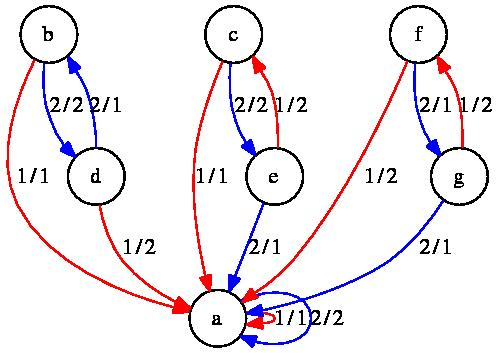
\includegraphics[height=4cm,keepaspectratio=true]{basilica-nucleus.jpg}   }

 

\subsection{\textcolor{Chapter }{Minimized (Mealy machine)}}
\logpage{[ 5, 2, 2 ]}\nobreak
\hyperdef{L}{X8395542D846FA2B9}{}
{\noindent\textcolor{FuncColor}{$\triangleright$\ \ \texttt{Minimized({\mdseries\slshape m})\index{Minimized@\texttt{Minimized}!Mealy machine}
\label{Minimized:Mealy machine}
}\hfill{\scriptsize (operation)}}\\
\textbf{\indent Returns:\ }
A minimized machine equivalent to \mbox{\texttt{\mdseries\slshape m}}.



 This function contructs the minimized Mealy machine \texttt{r} corresponding to \mbox{\texttt{\mdseries\slshape m}}, by identifying isomorphic states; and, if \mbox{\texttt{\mdseries\slshape m}} is initial, by removing inaccessible states. 

 If \mbox{\texttt{\mdseries\slshape m}} is initial, the minimized automaton is such that its states are numbered first
by distance to the initial state, and then lexicographically by input letter.
(in particular, the initial state is 1). This makes comparison of minimized
automata efficient. 

 Furthermore, \texttt{Correspondence(r)} is a list describing, for each (accessible) state of \mbox{\texttt{\mdseries\slshape m}}, its corresponding state in \texttt{r}; see \texttt{Correspondence} (\ref{Correspondence:FR machine}). 
\begin{Verbatim}[commandchars=!@|,fontsize=\small,frame=single,label=Example]
  !gapprompt@gap>| !gapinput@GrigorchukMachine := MealyMachine([[2,3],[4,4],[2,5],[4,4],[4,1]],|
                                         [(),(1,2),(),(),()]);
  <Mealy machine on alphabet [ 1, 2 ] with 5 states>
  !gapprompt@gap>| !gapinput@g2 := GrigorchukMachine^2;|
  <Mealy machine on alphabet [ 1, 2 ] with 25 states>
  !gapprompt@gap>| !gapinput@Minimized(g2);|
  <Mealy machine on alphabet [ 1, 2 ] with 11 states, minimized>
  !gapprompt@gap>| !gapinput@Correspondence(last);|
  [ 2, 1, 4, 11, 9, 1, 2, 5, 7, 6, 4, 3, 2, 9, 11, 11, 10, 9, 2, 4, 9, 8, 11, 4, 2 ]
  !gapprompt@gap>| !gapinput@e := FRElement(g2,11);|
  <Mealy element on alphabet [ 1, 2 ] with 25 states, initial state 11>
  !gapprompt@gap>| !gapinput@Minimized(e);|
  <Mealy element on alphabet [ 1, 2 ] with 5 states, initial state 1, minimized>
  !gapprompt@gap>| !gapinput@Correspondence(last);|
  [ 3, 2, 1, 4, 5, 2, 3,,,, 1,, 3, 5, 4, 4,, 5, 3, 1, 5,, 4, 1, 3 ]
\end{Verbatim}
 }

 

\subsection{\textcolor{Chapter }{DualMachine}}
\logpage{[ 5, 2, 3 ]}\nobreak
\hyperdef{L}{X809F069B798ED985}{}
{\noindent\textcolor{FuncColor}{$\triangleright$\ \ \texttt{DualMachine({\mdseries\slshape m})\index{DualMachine@\texttt{DualMachine}}
\label{DualMachine}
}\hfill{\scriptsize (operation)}}\\
\textbf{\indent Returns:\ }
The dual Mealy machine of \mbox{\texttt{\mdseries\slshape m}}.



 This function constructs the \emph{dual} machine of \mbox{\texttt{\mdseries\slshape m}}, i.e. the machine with stateset the alphabet of \mbox{\texttt{\mdseries\slshape m}}, with alphabet the stateset of \mbox{\texttt{\mdseries\slshape m}}, and similarly with transitions and output switched. 
\begin{Verbatim}[commandchars=!@|,fontsize=\small,frame=single,label=Example]
  !gapprompt@gap>| !gapinput@b := MealyMachine([[3,2],[3,1],[3,3]],[(1,2),(),()]);|
  <Mealy machine on alphabet [ 1, 2 ] with 3 states>
  !gapprompt@gap>| !gapinput@d := DualMachine(b)^4);|
  <Mealy machine on alphabet [ 1, 2, 3 ] with 16 states>
  !gapprompt@gap>| !gapinput@Draw(d); # action on 2^4 points|
  !gapprompt@gap>| !gapinput@DualMachine(d);|
  <Mealy machine on alphabet [ 1, 2, 3, 4, 5, 6, 7, 8, 9, 10, 11, 12, 13, 14, 15, 16
   ] with 3 states>
  !gapprompt@gap>| !gapinput@Output(last,1)=Activity(FRElement(b,1),4);|
  true
\end{Verbatim}
 }

 

\subsection{\textcolor{Chapter }{IsReversible}}
\logpage{[ 5, 2, 4 ]}\nobreak
\hyperdef{L}{X7D5D480C782FCC0B}{}
{\noindent\textcolor{FuncColor}{$\triangleright$\ \ \texttt{IsReversible({\mdseries\slshape m})\index{IsReversible@\texttt{IsReversible}}
\label{IsReversible}
}\hfill{\scriptsize (property)}}\\
\textbf{\indent Returns:\ }
\texttt{true} if \mbox{\texttt{\mdseries\slshape m}} is a reversible Mealy machine.



 This function tests whether \mbox{\texttt{\mdseries\slshape m}} is \emph{reversible}, i.e. whether the \texttt{DualMachine} (\ref{DualMachine}) of \mbox{\texttt{\mdseries\slshape m}} is invertible. See \cite{MR1841119} for more details. 
\begin{Verbatim}[commandchars=!@|,fontsize=\small,frame=single,label=Example]
  !gapprompt@gap>| !gapinput@IsReversible(MealyMachine([[1,2],[2,2]],[(1,2),()]));|
  false
  !gapprompt@gap>| !gapinput@IsReversible(MealyMachine([[1,2],[2,1]],[(),(1,2)]));|
\end{Verbatim}
 }

 

\subsection{\textcolor{Chapter }{IsMinimized}}
\logpage{[ 5, 2, 5 ]}\nobreak
\hyperdef{L}{X8310A1C08158793C}{}
{\noindent\textcolor{FuncColor}{$\triangleright$\ \ \texttt{IsMinimized({\mdseries\slshape m})\index{IsMinimized@\texttt{IsMinimized}}
\label{IsMinimized}
}\hfill{\scriptsize (property)}}\\
\textbf{\indent Returns:\ }
\texttt{true} if \mbox{\texttt{\mdseries\slshape m}} is a minimized Mealy machine.



 This function tests whether \mbox{\texttt{\mdseries\slshape m}} is \emph{minimized}, i.e. whether nono of its states can be removed or coalesced. All Mealy
elements are automatically minimized. 
\begin{Verbatim}[commandchars=!@|,fontsize=\small,frame=single,label=Example]
  !gapprompt@gap>| !gapinput@AllMealyMachines(2, 2, IsBireversible,EquivalenceClasses);|
  [ <Mealy machine on alphabet [ 1, 2 ] with 2 states>,
    <Mealy machine on alphabet [ 1, 2 ] with 2 states>,
    <Mealy machine on alphabet [ 1, 2 ] with 2 states>,
    <Mealy machine on alphabet [ 1, 2 ] with 2 states>,
    <Mealy machine on alphabet [ 1, 2 ] with 2 states>,
    <Mealy machine on alphabet [ 1, 2 ] with 2 states>,
    <Mealy machine on alphabet [ 1, 2 ] with 2 states>,
    <Mealy machine on alphabet [ 1, 2 ] with 2 states> ]
  !gapprompt@gap>| !gapinput@List(last,IsMinimized);|
  [ false, true, false, false, false, false, true, false ]
\end{Verbatim}
 }

 

\subsection{\textcolor{Chapter }{AlphabetInvolution}}
\logpage{[ 5, 2, 6 ]}\nobreak
\hyperdef{L}{X7CCB79B981912CCC}{}
{\noindent\textcolor{FuncColor}{$\triangleright$\ \ \texttt{AlphabetInvolution({\mdseries\slshape m})\index{AlphabetInvolution@\texttt{AlphabetInvolution}}
\label{AlphabetInvolution}
}\hfill{\scriptsize (attribute)}}\\
\textbf{\indent Returns:\ }
A list giving, for each alphabet letter, its inverse.



 If \mbox{\texttt{\mdseries\slshape m}} is a bireversible machine, it may happen that the stateset of the dual of \mbox{\texttt{\mdseries\slshape m}} (see \texttt{DualMachine} (\ref{DualMachine})) is closed under taking inverses. If this happens, then this list records the
mapping from an alphabet letter of \mbox{\texttt{\mdseries\slshape m}} to its inverse. 
\begin{Verbatim}[commandchars=!@|,fontsize=\small,frame=single,label=Example]
  !gapprompt@gap>| !gapinput@m := GammaPQMachine(3,5);; AlphabetOfFRObject(m);|
  [ 1 .. 6 ]
  !gapprompt@gap>| !gapinput@IsBireversible(m); AlphabetInvolution(GammaPQMachine(3,5));|
  true
  [ 6, 5, 4, 3, 2, 1 ]
\end{Verbatim}
 }

 

\subsection{\textcolor{Chapter }{IsBireversible}}
\logpage{[ 5, 2, 7 ]}\nobreak
\hyperdef{L}{X80D2545D7D0990A2}{}
{\noindent\textcolor{FuncColor}{$\triangleright$\ \ \texttt{IsBireversible({\mdseries\slshape m})\index{IsBireversible@\texttt{IsBireversible}}
\label{IsBireversible}
}\hfill{\scriptsize (property)}}\\
\textbf{\indent Returns:\ }
\texttt{true} if \mbox{\texttt{\mdseries\slshape m}} is a bireversible Mealy machine.



 This function tests whether \mbox{\texttt{\mdseries\slshape m}} is \emph{bireversible}, i.e. whether all eight machines obtained from \mbox{\texttt{\mdseries\slshape m}} using \texttt{DualMachine} (\ref{DualMachine}) and \texttt{Inverse} are well-defined. See \cite{MR1841119} for more details. 
\begin{Verbatim}[commandchars=!@|,fontsize=\small,frame=single,label=Example]
  !gapprompt@gap>| !gapinput@IsBireversible(MealyMachine([[1,2],[2,1]],[(),(1,2)]));|
  false
  !gapprompt@gap>| !gapinput@IsBireversible(MealyMachine([[1,1],[2,2]],[(),(1,2)]));|
  true
\end{Verbatim}
 }

 

\subsection{\textcolor{Chapter }{StateGrowth}}
\logpage{[ 5, 2, 8 ]}\nobreak
\hyperdef{L}{X83364DAB825D7A0D}{}
{\noindent\textcolor{FuncColor}{$\triangleright$\ \ \texttt{StateGrowth({\mdseries\slshape m[, x]})\index{StateGrowth@\texttt{StateGrowth}}
\label{StateGrowth}
}\hfill{\scriptsize (operation)}}\\
\textbf{\indent Returns:\ }
The state growth of the Mealy machine or element \mbox{\texttt{\mdseries\slshape m}}.



 This function computes, as a rational function, the power series in \mbox{\texttt{\mdseries\slshape x}} whose coefficient of degree $n$ is the number of non-trivial states at level $n$ of the tree. 

 If \mbox{\texttt{\mdseries\slshape x}} is absent, it is assumed to be \texttt{Indeterminate(Rationals)}. 

 If \mbox{\texttt{\mdseries\slshape m}} is a Mealy machine, this function is computed with respect to all possible
starting states. If \mbox{\texttt{\mdseries\slshape m}} is a Mealy element, this function is computed with respect to the initial
state of \mbox{\texttt{\mdseries\slshape m}}. 
\begin{Verbatim}[commandchars=!@|,fontsize=\small,frame=single,label=Example]
  !gapprompt@gap>| !gapinput@b := MealyMachine([[3,2],[3,1],[3,3]],[(1,2),(),()]);|
  <Mealy machine on alphabet [ 1, 2 ] with 3 states>
  !gapprompt@gap>| !gapinput@StateGrowth(b,Indeterminate(Rationals));|
  (2)/(-x_1+1)
  !gapprompt@gap>| !gapinput@StateGrowth(FRElement(b,1),Indeterminate(Rationals));|
  (1)/(-x_1+1)
\end{Verbatim}
 }

 

\subsection{\textcolor{Chapter }{Degree (FR element)}}
\logpage{[ 5, 2, 9 ]}\nobreak
\hyperdef{L}{X84BE780A81CAC69C}{}
{\noindent\textcolor{FuncColor}{$\triangleright$\ \ \texttt{Degree({\mdseries\slshape m})\index{Degree@\texttt{Degree}!FR element}
\label{Degree:FR element}
}\hfill{\scriptsize (operation)}}\\
\noindent\textcolor{FuncColor}{$\triangleright$\ \ \texttt{DegreeOfFRMachine({\mdseries\slshape m})\index{DegreeOfFRMachine@\texttt{DegreeOfFRMachine}}
\label{DegreeOfFRMachine}
}\hfill{\scriptsize (operation)}}\\
\noindent\textcolor{FuncColor}{$\triangleright$\ \ \texttt{DegreeOfFRElement({\mdseries\slshape m})\index{DegreeOfFRElement@\texttt{DegreeOfFRElement}}
\label{DegreeOfFRElement}
}\hfill{\scriptsize (operation)}}\\
\textbf{\indent Returns:\ }
The growth degree of the Mealy machine or element \mbox{\texttt{\mdseries\slshape m}}.



 This function computes the order of the pole at $x=1$ of \texttt{StateGrowth(m,x)}, in case its denominator is a product of cyclotomics; and returns \texttt{infinity} otherwise. 

 This attribute of Mealy machines was studied inter alia in \cite{MR1774362}. 
\begin{Verbatim}[commandchars=!@|,fontsize=\small,frame=single,label=Example]
  !gapprompt@gap>| !gapinput@m := MealyMachine([[2,1],[3,2],[3,3]],[(),(1,2),()]);|
  <Mealy machine on alphabet [ 1, 2 ] with 3 states>
  !gapprompt@gap>| !gapinput@StateGrowth(m,Indeterminate(Rationals));|
  (-x_1+2)/(x_1^2-2*x_1+1)
  !gapprompt@gap>| !gapinput@List(StateSet(m),i->Degree(FRElement(m,i)));|
  [ 2, 1, -1 ]
  !gapprompt@gap>| !gapinput@a := MealyMachine(Group((1,2)),Group((1,2)),\*,\*);|
  <Mealy machine on alphabet [ (), (1,2) ] with states Group( [ (1,2) ] )>
  !gapprompt@gap>| !gapinput@Degree(a);|
  infinity
\end{Verbatim}
 }

 

\subsection{\textcolor{Chapter }{IsFinitaryFRElement}}
\logpage{[ 5, 2, 10 ]}\nobreak
\hyperdef{L}{X793C427084F830CE}{}
{\noindent\textcolor{FuncColor}{$\triangleright$\ \ \texttt{IsFinitaryFRElement({\mdseries\slshape e})\index{IsFinitaryFRElement@\texttt{IsFinitaryFRElement}}
\label{IsFinitaryFRElement}
}\hfill{\scriptsize (property)}}\\
\noindent\textcolor{FuncColor}{$\triangleright$\ \ \texttt{IsFinitaryFRMachine({\mdseries\slshape e})\index{IsFinitaryFRMachine@\texttt{IsFinitaryFRMachine}}
\label{IsFinitaryFRMachine}
}\hfill{\scriptsize (property)}}\\
\textbf{\indent Returns:\ }
\texttt{true} if \mbox{\texttt{\mdseries\slshape e}} is a finitary element.



 This function tests whether \mbox{\texttt{\mdseries\slshape e}} is a finitary element. These are by definition the elements of growth degree
at most $0$. 

 When applied to a Mealy machine, it returns \texttt{true} if all states of \mbox{\texttt{\mdseries\slshape e}} are finitary. 
\begin{Verbatim}[commandchars=!@A,fontsize=\small,frame=single,label=Example]
  !gapprompt@gap>A !gapinput@m := GuptaSidkiMachines(3);; Display(m);A
     |  1     2     3
  ---+-----+-----+-----+
   a | a,1   a,2   a,3
   b | a,2   a,3   a,1
   c | a,3   a,1   a,2
   d | b,1   c,2   d,3
  ---+-----+-----+-----+
  !gapprompt@gap>A !gapinput@Filtered(StateSet(m),i->IsFinitaryFRElement(FRElement(m,i)));A
  [ 1, 2, 3 ]
  !gapprompt@gap>A !gapinput@IsFinitaryFRElement(m);A
  false
\end{Verbatim}
 }

 

\subsection{\textcolor{Chapter }{Depth (FR element)}}
\logpage{[ 5, 2, 11 ]}\nobreak
\hyperdef{L}{X7E5E8B2C79688DC0}{}
{\noindent\textcolor{FuncColor}{$\triangleright$\ \ \texttt{Depth({\mdseries\slshape m})\index{Depth@\texttt{Depth}!FR element}
\label{Depth:FR element}
}\hfill{\scriptsize (attribute)}}\\
\noindent\textcolor{FuncColor}{$\triangleright$\ \ \texttt{DepthOfFRMachine({\mdseries\slshape m})\index{DepthOfFRMachine@\texttt{DepthOfFRMachine}}
\label{DepthOfFRMachine}
}\hfill{\scriptsize (attribute)}}\\
\noindent\textcolor{FuncColor}{$\triangleright$\ \ \texttt{DepthOfFRElement({\mdseries\slshape m})\index{DepthOfFRElement@\texttt{DepthOfFRElement}}
\label{DepthOfFRElement}
}\hfill{\scriptsize (attribute)}}\\
\textbf{\indent Returns:\ }
The depth of the finitary Mealy machine or element \mbox{\texttt{\mdseries\slshape m}}.



 This function computes the maximal level at which the \mbox{\texttt{\mdseries\slshape m}} has an non-trivial state. In particular the identity has depth 0, and FR
elements acting only at the root vertex have depth 1. The value \texttt{infinity} is returned if \mbox{\texttt{\mdseries\slshape m}} is not finitary (see \texttt{IsFinitaryFRElement} (\ref{IsFinitaryFRElement})). 
\begin{Verbatim}[commandchars=!@|,fontsize=\small,frame=single,label=Example]
  !gapprompt@gap>| !gapinput@m := MealyMachine([[2,1],[3,3],[4,4],[4,4]],[(),(),(1,2),()]);|
  <Mealy machine on alphabet [ 1, 2 ] with 4 states>
  !gapprompt@gap>| !gapinput@DepthOfFRMachine(m);|
  infinity
  !gapprompt@gap>| !gapinput@List(StateSet(m),i->DepthOfFRElement(FRElement(m,i)));|
  [ infinity, 2, 1, 0 ]
\end{Verbatim}
 }

 

\subsection{\textcolor{Chapter }{IsBoundedFRElement}}
\logpage{[ 5, 2, 12 ]}\nobreak
\hyperdef{L}{X82F4410E85C54C7E}{}
{\noindent\textcolor{FuncColor}{$\triangleright$\ \ \texttt{IsBoundedFRElement({\mdseries\slshape e})\index{IsBoundedFRElement@\texttt{IsBoundedFRElement}}
\label{IsBoundedFRElement}
}\hfill{\scriptsize (property)}}\\
\noindent\textcolor{FuncColor}{$\triangleright$\ \ \texttt{IsBoundedFRMachine({\mdseries\slshape e})\index{IsBoundedFRMachine@\texttt{IsBoundedFRMachine}}
\label{IsBoundedFRMachine}
}\hfill{\scriptsize (property)}}\\
\textbf{\indent Returns:\ }
\texttt{true} if \mbox{\texttt{\mdseries\slshape e}} is a finitary element.



 This function tests whether \mbox{\texttt{\mdseries\slshape e}} is a bounded element. These are by definition the elements of growth degree at
most $1$. 

 When applied to a Mealy machine, it returns \texttt{true} if all states of \mbox{\texttt{\mdseries\slshape e}} are bounded. 
\begin{Verbatim}[commandchars=!@A,fontsize=\small,frame=single,label=Example]
  !gapprompt@gap>A !gapinput@m := GuptaSidkiMachines(3);; Display(m);A
     |  1     2     3
  ---+-----+-----+-----+
   a | a,1   a,2   a,3
   b | a,2   a,3   a,1
   c | a,3   a,1   a,2
   d | b,1   c,2   d,3
  ---+-----+-----+-----+
  !gapprompt@gap>A !gapinput@Filtered(StateSet(m),i->IsBoundedFRElement(FRElement(m,i)));A
  [ 1, 2, 3, 4 ]
  !gapprompt@gap>A !gapinput@IsBoundedFRMachine(m);A
  true
\end{Verbatim}
 }

 

\subsection{\textcolor{Chapter }{IsPolynomialGrowthFRElement}}
\logpage{[ 5, 2, 13 ]}\nobreak
\hyperdef{L}{X81D4A3F27C5FAD96}{}
{\noindent\textcolor{FuncColor}{$\triangleright$\ \ \texttt{IsPolynomialGrowthFRElement({\mdseries\slshape e})\index{IsPolynomialGrowthFRElement@\texttt{IsPolynomialGrowthFRElement}}
\label{IsPolynomialGrowthFRElement}
}\hfill{\scriptsize (property)}}\\
\noindent\textcolor{FuncColor}{$\triangleright$\ \ \texttt{IsPolynomialGrowthFRMachine({\mdseries\slshape e})\index{IsPolynomialGrowthFRMachine@\texttt{IsPolynomialGrowthFRMachine}}
\label{IsPolynomialGrowthFRMachine}
}\hfill{\scriptsize (property)}}\\
\textbf{\indent Returns:\ }
\texttt{true} if \mbox{\texttt{\mdseries\slshape e}} is an element of polynomial growth.



 This function tests whether \mbox{\texttt{\mdseries\slshape e}} is a polynomial element. These are by definition the elements of polynomial
growth degree. 

 When applied to a Mealy machine, it returns \texttt{true} if all states of \mbox{\texttt{\mdseries\slshape e}} are of polynomial growth. 
\begin{Verbatim}[commandchars=!@A,fontsize=\small,frame=single,label=Example]
  !gapprompt@gap>A !gapinput@m := GuptaSidkiMachines(3);; Display(m);A
     |  1     2     3
  ---+-----+-----+-----+
   a | a,1   a,2   a,3
   b | a,2   a,3   a,1
   c | a,3   a,1   a,2
   d | b,1   c,2   d,3
  ---+-----+-----+-----+
  !gapprompt@gap>A !gapinput@Filtered(StateSet(m),i->IsPolynomialGrowthFRElement(FRElement(m,i)));A
  [ 1, 2, 3, 4 ]
  !gapprompt@gap>A !gapinput@IsPolynomialGrowthFRMachine(m);A
  true
\end{Verbatim}
 }

 

\subsection{\textcolor{Chapter }{Signatures}}
\logpage{[ 5, 2, 14 ]}\nobreak
\hyperdef{L}{X7ECE17387910C023}{}
{\noindent\textcolor{FuncColor}{$\triangleright$\ \ \texttt{Signatures({\mdseries\slshape e})\index{Signatures@\texttt{Signatures}}
\label{Signatures}
}\hfill{\scriptsize (operation)}}\\
\textbf{\indent Returns:\ }
A list describing the product of the activities on each level.



 This function computes the product of the activities of \mbox{\texttt{\mdseries\slshape e}} on each level, and returns a periodic list describing it (see \texttt{PeriodicList} (\ref{PeriodicList})). 

 The entries \texttt{pi} are permutations, and their values are meaningful only when projected in the
abelianization of \texttt{VertexTransformationsFRElement(e)}. 
\begin{Verbatim}[commandchars=!@|,fontsize=\small,frame=single,label=Example]
  !gapprompt@gap>| !gapinput@Signatures(GrigorchukGroup.1);|
  [ (1,2), / () ]
  !gapprompt@gap>| !gapinput@Signatures(GrigorchukGroup.2);|
  [/ (), (1,2), (1,2) ]
  !gapprompt@gap>| !gapinput@last[50];|
  (1,2)
  !gapprompt@gap>| !gapinput@Signatures(AddingMachine(3)[2]);|
  [/ (1,2,3) ]
\end{Verbatim}
 }

 

\subsection{\textcolor{Chapter }{VertexTransformationsFRMachine}}
\logpage{[ 5, 2, 15 ]}\nobreak
\hyperdef{L}{X83DFDC3384EA4634}{}
{\noindent\textcolor{FuncColor}{$\triangleright$\ \ \texttt{VertexTransformationsFRMachine({\mdseries\slshape m})\index{VertexTransformationsFRMachine@\texttt{VertexTransformationsFRMachine}}
\label{VertexTransformationsFRMachine}
}\hfill{\scriptsize (operation)}}\\
\noindent\textcolor{FuncColor}{$\triangleright$\ \ \texttt{VertexTransformationsFRElement({\mdseries\slshape e})\index{VertexTransformationsFRElement@\texttt{VertexTransformationsFRElement}}
\label{VertexTransformationsFRElement}
}\hfill{\scriptsize (operation)}}\\
\textbf{\indent Returns:\ }
The group/monoid generated by all vertex transformations of states of \mbox{\texttt{\mdseries\slshape m}}.



 The first function computes the finite permutation group / transformation
monoid generated by all outputs of states of \mbox{\texttt{\mdseries\slshape m}}. 

 The second command is a short-hand for \texttt{VertexTransformationsFRMachine(UnderlyingFRMachine(e))}. 
\begin{Verbatim}[commandchars=!@|,fontsize=\small,frame=single,label=Example]
  !gapprompt@gap>| !gapinput@m := MealyMachine([[1,3,2],[3,2,1],[2,1,3]],[(2,3),(1,3),(1,2)]);|
  <Mealy machine on alphabet [ 1, 2 ] with 3 states>
  !gapprompt@gap>| !gapinput@VertexTransformationsFRMachine(m);|
  Group([ (2,3), (1,3), (1,2) ])
\end{Verbatim}
 }

 

\subsection{\textcolor{Chapter }{FixedRay (FR element)}}
\logpage{[ 5, 2, 16 ]}\nobreak
\hyperdef{L}{X7E0CB3767CE08692}{}
{\noindent\textcolor{FuncColor}{$\triangleright$\ \ \texttt{FixedRay({\mdseries\slshape e})\index{FixedRay@\texttt{FixedRay}!FR element}
\label{FixedRay:FR element}
}\hfill{\scriptsize (operation)}}\\
\textbf{\indent Returns:\ }
The lexicographically first ray fixed by \mbox{\texttt{\mdseries\slshape e}}.



 This function computes the lexicographically first infinite sequence that is
fixed by the FR element \mbox{\texttt{\mdseries\slshape e}}, and returns it as a periodic list (see \texttt{PeriodicList} (\ref{PeriodicList})). It returns \texttt{fail} if no such ray exists. 
\begin{Verbatim}[commandchars=!@|,fontsize=\small,frame=single,label=Example]
  !gapprompt@gap>| !gapinput@m := MealyMachine([[1,3,2],[3,2,1],[2,1,3]],[(2,3),(1,3),(1,2)]);|
  <Mealy machine on alphabet [ 1, 2 ] with 3 states>
  !gapprompt@gap>| !gapinput@FixedRay(FRElement(m,1));|
  [/ 1 ]
  !gapprompt@gap>| !gapinput@last^FRElement(m,1);|
  [/ 1 ]
  !gapprompt@gap>| !gapinput@FixedRay(FRElement(m,[1,2]));|
  fail
\end{Verbatim}
 }

 

\subsection{\textcolor{Chapter }{IsLevelTransitive (FR element)}}
\logpage{[ 5, 2, 17 ]}\nobreak
\hyperdef{L}{X828C167B7D7691E9}{}
{\noindent\textcolor{FuncColor}{$\triangleright$\ \ \texttt{IsLevelTransitive({\mdseries\slshape e})\index{IsLevelTransitive@\texttt{IsLevelTransitive}!FR element}
\label{IsLevelTransitive:FR element}
}\hfill{\scriptsize (property)}}\\
\textbf{\indent Returns:\ }
\texttt{true} if \mbox{\texttt{\mdseries\slshape e}} acts transitively on each level of the tree.



 This function tests whether \mbox{\texttt{\mdseries\slshape e}} acts transitively on each level of the tree. It is implemented only if \texttt{VertexTransformationsFRElement(e)} is abelian. 

 This function is used as a simple test to detect whether an element has
infinite order: if \mbox{\texttt{\mdseries\slshape e}} has a fixed vertex $v$ such that the \texttt{State(e,v)} is level-transitive, then \mbox{\texttt{\mdseries\slshape e}} has infinite order. 
\begin{Verbatim}[commandchars=!@B,fontsize=\small,frame=single,label=Example]
  !gapprompt@gap>B !gapinput@m := AddingMachine(3);; Display(m);B
     |  1     2     3
  ---+-----+-----+-----+
   a | a,1   a,2   a,3
   b | a,2   a,3   b,1
  ---+-----+-----+-----+
  Initial state:  b
  !gapprompt@gap>B !gapinput@IsLevelTransitive(m);B
  true
  !gapprompt@gap>B !gapinput@IsLevelTransitive(Product(UnderlyingFRMachine(GrigorchukOverGroup){[2..5]}));B
  true
\end{Verbatim}
 }

 

\subsection{\textcolor{Chapter }{AsMealyMachine (FR machine)}}
\logpage{[ 5, 2, 18 ]}\nobreak
\hyperdef{L}{X79EFE2C97D2CCEEC}{}
{\noindent\textcolor{FuncColor}{$\triangleright$\ \ \texttt{AsMealyMachine({\mdseries\slshape m})\index{AsMealyMachine@\texttt{AsMealyMachine}!FR machine}
\label{AsMealyMachine:FR machine}
}\hfill{\scriptsize (attribute)}}\\
\textbf{\indent Returns:\ }
A Mealy machine isomorphic to \mbox{\texttt{\mdseries\slshape m}}.



 This function constructs a Mealy machine \texttt{r}, which is as close as possible to the FR machine \mbox{\texttt{\mdseries\slshape m}}. Furthermore, \texttt{Correspondence(r)} is a list identifying, for every generator of the stateset of \mbox{\texttt{\mdseries\slshape m}}, a corresponding state in the new Mealy machine; see \texttt{Correspondence} (\ref{Correspondence:FR machine}). 

 \mbox{\texttt{\mdseries\slshape m}} may be a group/monoid/semigroup FR machine, or a Mealy machine; in which case
the result is returned unchanged. 

 In particular, \texttt{FRElement(m,s)} and \texttt{FRElement(AsMealyMachine(m),s)} return the same tree automorphism, for any FR machine \texttt{m} and any state \texttt{s}. 

 This function is not guaranteed to return; if \mbox{\texttt{\mdseries\slshape m}} does not have finite states, then it will loop forever. 
\begin{Verbatim}[commandchars=!@B,fontsize=\small,frame=single,label=Example]
  !gapprompt@gap>B !gapinput@n := FRMachine(["tau","mu"],[[[],[1]],[[],[-2]]],[(1,2),(1,2)]);B
  <FR machine with alphabet [ 1 .. 2 ] on Group( [ tau, mu ] )>
  !gapprompt@gap>B !gapinput@Display(n);B
       |     1         2
  -----+--------+---------+
   tau | <id>,2     tau,1
    mu | <id>,2   mu^-1,1
  -----+--------+---------+
  !gapprompt@gap>B !gapinput@AsMealyMachine(n);B
  <Mealy machine on alphabet [ 1, 2 ] with 4 states>
  !gapprompt@gap>B !gapinput@Display(last);B
     |  1     2
  ---+-----+-----+
   a | c,2   a,1
   b | c,2   d,1
   c | c,1   c,2
   d | b,2   c,1
  ---+-----+-----+
  !gapprompt@gap>B !gapinput@Correspondence(last);B
  [ 1, 2 ]
\end{Verbatim}
 }

 

\subsection{\textcolor{Chapter }{AsMealyMachine (List)}}
\logpage{[ 5, 2, 19 ]}\nobreak
\hyperdef{L}{X80F9A18483F98442}{}
{\noindent\textcolor{FuncColor}{$\triangleright$\ \ \texttt{AsMealyMachine({\mdseries\slshape l})\index{AsMealyMachine@\texttt{AsMealyMachine}!List}
\label{AsMealyMachine:List}
}\hfill{\scriptsize (attribute)}}\\
\textbf{\indent Returns:\ }
A Mealy machine constructed out of the FR elements in \mbox{\texttt{\mdseries\slshape l}}.



 This function constructs a Mealy machine \texttt{r}, with states \mbox{\texttt{\mdseries\slshape l}} (which must be a state-closed set). Its outputs are the outputs of its
elements, and its transitions are the transitions of its elements; in
particular, \texttt{FRElement(r,i)} is equal to \texttt{l[i]} as an FR element. 

 \texttt{Correspondence(r)} records the argument \mbox{\texttt{\mdseries\slshape l}}. 

 This function returns \texttt{fail} if \mbox{\texttt{\mdseries\slshape l}} is not state-closed. 
\begin{Verbatim}[commandchars=!@B,fontsize=\small,frame=single,label=Example]
  !gapprompt@gap>B !gapinput@ mu := FRElement([[[],[-1]]],[(1,2)],[1]);B
  <2|f1>
  gap>
  !gapprompt@gap>B !gapinput@States(mu);B
  [ <2|f1>, <2|identity ...>, <2|f1^-1> ]
  !gapprompt@gap>B !gapinput@AsMealyMachine(last);B
  <Mealy machine on alphabet [ 1, 2 ] with 3 states>
  !gapprompt@gap>B !gapinput@Display(last);B
     |  1     2
  ---+-----+-----+
   a | b,2   c,1
   b | b,1   b,2
   c | a,2   b,1
  ---+-----+-----+
\end{Verbatim}
 }

 

\subsection{\textcolor{Chapter }{AsMealyElement}}
\logpage{[ 5, 2, 20 ]}\nobreak
\hyperdef{L}{X7FB3F0A2878DD2CF}{}
{\noindent\textcolor{FuncColor}{$\triangleright$\ \ \texttt{AsMealyElement({\mdseries\slshape m})\index{AsMealyElement@\texttt{AsMealyElement}}
\label{AsMealyElement}
}\hfill{\scriptsize (attribute)}}\\
\textbf{\indent Returns:\ }
A Mealy element isomorphic to \mbox{\texttt{\mdseries\slshape m}}.



 This function constructs a Mealy element, which induces the same tree
automorphism as the FR element \mbox{\texttt{\mdseries\slshape m}}. 

 \mbox{\texttt{\mdseries\slshape m}} may be a group/monoid/semigroup FR element, or a Mealy element; in which case
the result is returned unchanged. 

 This function is not guaranteed to return; if \mbox{\texttt{\mdseries\slshape m}} does not have finite states, then it will loop forever. 
\begin{Verbatim}[commandchars=!@B,fontsize=\small,frame=single,label=Example]
  !gapprompt@gap>B !gapinput@mu := FRElement([[[],[-1]]],[(1,2)],[1]);B
  <2|f1>
  !gapprompt@gap>B !gapinput@AsMealyElement(mu);B
  <Mealy machine on alphabet [ 1, 2 ] with 3 states, initial state 1>
  !gapprompt@gap>B !gapinput@[[2,1]]^last;B
  [ [ 1, 2 ] ]
  !gapprompt@gap>B !gapinput@[2,1,2,1]^mu;B
  [ 1, 2, 1, 2 ]
\end{Verbatim}
 }

 

\subsection{\textcolor{Chapter }{AsIntMealyMachine}}
\logpage{[ 5, 2, 21 ]}\nobreak
\hyperdef{L}{X7FBBBD9A839011C8}{}
{\noindent\textcolor{FuncColor}{$\triangleright$\ \ \texttt{AsIntMealyMachine({\mdseries\slshape m})\index{AsIntMealyMachine@\texttt{AsIntMealyMachine}}
\label{AsIntMealyMachine}
}\hfill{\scriptsize (attribute)}}\\
\noindent\textcolor{FuncColor}{$\triangleright$\ \ \texttt{AsIntMealyElement({\mdseries\slshape m})\index{AsIntMealyElement@\texttt{AsIntMealyElement}}
\label{AsIntMealyElement}
}\hfill{\scriptsize (attribute)}}\\
\textbf{\indent Returns:\ }
A Mealy machine in integer format, isomorphic to \mbox{\texttt{\mdseries\slshape m}}.



 This function constructs a Mealy machine \texttt{r}, which has similar behaviour as \mbox{\texttt{\mdseries\slshape m}} while having stateset \texttt{[1..n]} for some natural \texttt{n}. Most \textsf{FR} commands operate efficiently only on Mealy machines of this type. 

 This function is not guaranteed to return; if \mbox{\texttt{\mdseries\slshape m}} does not have finite states, then it will loop forever. 
\begin{Verbatim}[commandchars=!@B,fontsize=\small,frame=single,label=Example]
  !gapprompt@gap>B !gapinput@g := Group((1,2));; n := MealyMachine(g,g,\*,\*);B
  <Mealy machine on alphabet [ (), (1,2) ] with states Group( [ (1,2) ] )>
  !gapprompt@gap>B !gapinput@Display(n);B
         |      ()            (1,2)
  -------+-------------+-------------+
      () |    (),()      (1,2),(1,2)
   (1,2) | (1,2),(1,2)      (),()
  -------+-------------+-------------+
  !gapprompt@gap>B !gapinput@AsIntMealyMachine(n);B
  <Mealy machine on alphabet [ 1, 2 ] with 2 states>
  !gapprompt@gap>B !gapinput@Display(last);B
     |  1     2
  ---+-----+-----+
   a | a,1   b,2
   b | b,2   a,1
  ---+-----+-----+
  !gapprompt@gap>B !gapinput@Correspondence(last);B
  [ 1, 2 ]
\end{Verbatim}
 }

 

\subsection{\textcolor{Chapter }{TopElement}}
\logpage{[ 5, 2, 22 ]}\nobreak
\hyperdef{L}{X8191456B7E586785}{}
{\noindent\textcolor{FuncColor}{$\triangleright$\ \ \texttt{TopElement({\mdseries\slshape p[, n]})\index{TopElement@\texttt{TopElement}}
\label{TopElement}
}\hfill{\scriptsize (attribute)}}\\
\textbf{\indent Returns:\ }
A Mealy machine in integer format, acting on the first symbol of sequences.



 This function constructs a Mealy machine \texttt{r}, which acts as \mbox{\texttt{\mdseries\slshape p}} on the first letter of sequences and fixes the other letters. The argument \mbox{\texttt{\mdseries\slshape n}} is the size of the alphabet of \texttt{r}; if it is ommitted, then it is assumed to be the degree of the transformation \mbox{\texttt{\mdseries\slshape p}}, or the largest moved point of the permutation or trans \mbox{\texttt{\mdseries\slshape p}}. 
\begin{Verbatim}[commandchars=!@|,fontsize=\small,frame=single,label=Example]
  !gapprompt@gap>| !gapinput@a := TopElement((1,2));|
  <Mealy element on alphabet [ 1, 2 ] with 2 states>
  !gapprompt@gap>| !gapinput@last=GrigorchukGroup.1;|
  true
  !gapprompt@gap>| !gapinput@a := TopElement((1,2),3);|
  <Mealy element on alphabet [ 1, 2, 3 ] with 2 states>
  !gapprompt@gap>| !gapinput@last in GuptaSidkiGroup;|
  false
\end{Verbatim}
 }

 

\subsection{\textcolor{Chapter }{ConfinalityClasses}}
\logpage{[ 5, 2, 23 ]}\nobreak
\hyperdef{L}{X7A87ED9D789245E4}{}
{\noindent\textcolor{FuncColor}{$\triangleright$\ \ \texttt{ConfinalityClasses({\mdseries\slshape e})\index{ConfinalityClasses@\texttt{ConfinalityClasses}}
\label{ConfinalityClasses}
}\hfill{\scriptsize (attribute)}}\\
\noindent\textcolor{FuncColor}{$\triangleright$\ \ \texttt{IsWeaklyFinitaryFRElement({\mdseries\slshape e})\index{IsWeaklyFinitaryFRElement@\texttt{IsWeaklyFinitaryFRElement}}
\label{IsWeaklyFinitaryFRElement}
}\hfill{\scriptsize (attribute)}}\\
\textbf{\indent Returns:\ }
A list describing the non-trivial confinality classes of \mbox{\texttt{\mdseries\slshape e}}.



 If \mbox{\texttt{\mdseries\slshape e}} is a bounded element (see \texttt{IsBoundedFRElement} (\ref{IsBoundedFRElement})), there are finitely many infinite sequences that have confinality class
larger that one; i.e. ultimately periodic sequences that are mapped by \mbox{\texttt{\mdseries\slshape e}} to a sequence with different period. This function returns a list of
equivalence classes of periodic lists, see \texttt{PeriodicList} (\ref{PeriodicList}), which are related under \mbox{\texttt{\mdseries\slshape e}}. 

 By definition, an element is \emph{weakly finitary} if it has no non-singleton confinality classes. 
\begin{Verbatim}[commandchars=!@|,fontsize=\small,frame=single,label=Example]
  !gapprompt@gap>| !gapinput@g := FRGroup("t=<,,t>(2,3)","u=<u,,>(1,2)","v=<u,t,>");;|
  !gapprompt@gap>| !gapinput@ConfinalityClasses(g.1);|
  [ {PeriodicList([  ],[ 2 ])} ]
  !gapprompt@gap>| !gapinput@List(GeneratorsOfGroup(g),x->Elements(ConfinalityClasses(x)[1]));|
  [ [ [/ 2 ], [/ 3 ] ],
    [ [/ 1 ], [/ 2 ] ],
    [ [/ 1 ], [/ 2 ], [/ 3 ] ] ]
  !gapprompt@gap>| !gapinput@IsWeaklyFinitaryFRElement(BinaryAddingElement);|
  false
  !gapprompt@gap>| !gapinput@IsWeaklyFinitaryFRElement(GuptaSidkiGroup.2);|
  true
\end{Verbatim}
 }

 

\subsection{\textcolor{Chapter }{Germs}}
\logpage{[ 5, 2, 24 ]}\nobreak
\hyperdef{L}{X81592E3D79745A40}{}
{\noindent\textcolor{FuncColor}{$\triangleright$\ \ \texttt{Germs({\mdseries\slshape e})\index{Germs@\texttt{Germs}}
\label{Germs}
}\hfill{\scriptsize (attribute)}}\\
\noindent\textcolor{FuncColor}{$\triangleright$\ \ \texttt{NormOfBoundedFRElement({\mdseries\slshape e})\index{NormOfBoundedFRElement@\texttt{NormOfBoundedFRElement}}
\label{NormOfBoundedFRElement}
}\hfill{\scriptsize (attribute)}}\\
\textbf{\indent Returns:\ }
The germs of the bounded element \mbox{\texttt{\mdseries\slshape e}}.



 The \emph{germs} of a bounded element are the finitely many ultimately periodic sequences on
which the state of \mbox{\texttt{\mdseries\slshape e}} does not vanish. This function returns the germs of \mbox{\texttt{\mdseries\slshape e}}, as a list of pairs; the first entry is a ray described as a periodic
sequence of integers (see \texttt{PeriodicList} (\ref{PeriodicList})), and the second entry is the periodic sequence of states that appear along
that ray. 

 The \emph{norm} of a bounded element is the length of its list of germs. 
\begin{Verbatim}[commandchars=!@C,fontsize=\small,frame=single,label=Example]
  !gapprompt@gap>C !gapinput@Germs(BinaryAddingElement);C
  [ [ [/ 2 ], [/ 1 ] ] ]
  !gapprompt@gap>C !gapinput@Germs(GrigorchukGroup.1);C
  [  ]
  !gapprompt@gap>C !gapinput@Germs(GrigorchukGroup.2);C
  [ [ [/ 2 ], [/ 1, 3, 5 ] ] ]
  !gapprompt@gap>C !gapinput@Display(GrigorchukGroup.2);C
     |  1     2
  ---+-----+-----+
   a | b,1   c,2
   b | d,2   d,1
   c | b,1   e,2
   d | d,1   d,2
   e | d,1   a,2
  ---+-----+-----+
  Initial state: a
\end{Verbatim}
 }

 

\subsection{\textcolor{Chapter }{HasOpenSetConditionFRElement}}
\logpage{[ 5, 2, 25 ]}\nobreak
\hyperdef{L}{X7F76AF2D7C0279F9}{}
{\noindent\textcolor{FuncColor}{$\triangleright$\ \ \texttt{HasOpenSetConditionFRElement({\mdseries\slshape e})\index{HasOpenSetConditionFRElement@\texttt{HasOpenSetConditionFRElement}}
\label{HasOpenSetConditionFRElement}
}\hfill{\scriptsize (property)}}\\
\textbf{\indent Returns:\ }
\texttt{true} if \mbox{\texttt{\mdseries\slshape e}} has the open set condition.



 An FR element \mbox{\texttt{\mdseries\slshape e}} has the \emph{open set condition} if for every infinite ray in the tree which is fixed by \mbox{\texttt{\mdseries\slshape e}}, there is an open set around that ray which is also fixed by \mbox{\texttt{\mdseries\slshape e}}. This function tests for \mbox{\texttt{\mdseries\slshape e}} to have the open set condition. It currently is implemented only for bounded
elements. 
\begin{Verbatim}[commandchars=!@|,fontsize=\small,frame=single,label=Example]
  !gapprompt@gap>| !gapinput@HasOpenSetConditionFRElement(GrigorchukGroup.1);|
  true
  !gapprompt@gap>| !gapinput@HasOpenSetConditionFRElement(GrigorchukGroup.2);|
  false
\end{Verbatim}
 }

 

\subsection{\textcolor{Chapter }{LimitFRMachine}}
\logpage{[ 5, 2, 26 ]}\nobreak
\hyperdef{L}{X795017598575FCA3}{}
{\noindent\textcolor{FuncColor}{$\triangleright$\ \ \texttt{LimitFRMachine({\mdseries\slshape m})\index{LimitFRMachine@\texttt{LimitFRMachine}}
\label{LimitFRMachine}
}\hfill{\scriptsize (attribute)}}\\
\textbf{\indent Returns:\ }
The submachine of \mbox{\texttt{\mdseries\slshape m}} on all recurrent states.



 This command creates a new Mealy machine, with stateset the limit states of \mbox{\texttt{\mdseries\slshape m}}. 
\begin{Verbatim}[commandchars=!@A,fontsize=\small,frame=single,label=Example]
  !gapprompt@gap>A !gapinput@m := MealyMachine([[2,2,3],[2,3,3],[3,3,3]],[(),(),(1,2,3)]);A
  <Mealy machine on alphabet [ 1 .. 3 ] with 3 states>
  !gapprompt@gap>A !gapinput@Display(m);A
     |  1     2     3
  ---+-----+-----+-----+
   a | b,1   b,2   c,3
   b | b,1   c,2   c,3
   c | c,2   c,3   c,1
  ---+-----+-----+-----+
  !gapprompt@gap>A !gapinput@LimitStates(m);A
  [ <Mealy element on alphabet [ 1 .. 3 ] with 2 states>,
    <Mealy element on alphabet [ 1 .. 3 ] with 1 state> ]
  !gapprompt@gap>A !gapinput@LimitFRMachine(m);A
  <Mealy machine on alphabet [ 1 .. 3 ] with 2 states>
  !gapprompt@gap>A !gapinput@Display(last);A
     |  1     2     3
  ---+-----+-----+-----+
   a | a,1   b,2   b,3
   b | b,2   b,3   b,1
  ---+-----+-----+-----+
\end{Verbatim}
 }

 

\subsection{\textcolor{Chapter }{NucleusMachine (FR machine)}}
\logpage{[ 5, 2, 27 ]}\nobreak
\hyperdef{L}{X7F8163B5816969C8}{}
{\noindent\textcolor{FuncColor}{$\triangleright$\ \ \texttt{NucleusMachine({\mdseries\slshape m})\index{NucleusMachine@\texttt{NucleusMachine}!FR machine}
\label{NucleusMachine:FR machine}
}\hfill{\scriptsize (attribute)}}\\
\textbf{\indent Returns:\ }
The nucleus of \mbox{\texttt{\mdseries\slshape m}}.



 This command creates a new Mealy machine \texttt{n}, with stateset the nucleus (see \texttt{NucleusOfFRMachine} (\ref{NucleusOfFRMachine})) of \mbox{\texttt{\mdseries\slshape m}}. 

 This nucleus machine is characterized as the smallest machine \texttt{n} such that \texttt{Minimized(LimitFRMachine(m*n))} is isomorphic to \texttt{n}. It is also isomorphic to the \texttt{NucleusMachine} (\ref{NucleusMachine:FR semigroup}) of the state closure of the \texttt{SCSemigroup} (\ref{SCSemigroup}) of \mbox{\texttt{\mdseries\slshape m}}. 

 Note that the ordering of the states in the resulting machine is not
necessarily the same as in \mbox{\texttt{\mdseries\slshape m}}; however, if \mbox{\texttt{\mdseries\slshape m}} and \texttt{n} are isomorphic, then this command returns \mbox{\texttt{\mdseries\slshape m}}. 
\begin{Verbatim}[commandchars=!@A,fontsize=\small,frame=single,label=Example]
  !gapprompt@gap>A !gapinput@m := MealyMachine([[2,1,1],[2,2,2]],[(1,2,3),()]);A
  <Mealy machine on alphabet [ 1, 2, 3 ] with 2 states>
  !gapprompt@gap>A !gapinput@Display(m);A
     |  1     2     3
  ---+-----+-----+-----+
   a | b,2   a,3   a,1
   b | b,1   b,2   b,3
  ---+-----+-----+-----+
  !gapprompt@gap>A !gapinput@NucleusMachine(m);A
  <Mealy machine on alphabet [ 1, 2, 3 ] with 3 states>
  !gapprompt@gap>A !gapinput@Display(last);A
     |  1     2     3
  ---+-----+-----+-----+
   a | a,1   a,2   a,3
   b | c,3   b,1   c,2
   c | a,2   c,3   c,1
  ---+-----+-----+-----+
\end{Verbatim}
 }

 

\subsection{\textcolor{Chapter }{GuessMealyElement}}
\logpage{[ 5, 2, 28 ]}\nobreak
\hyperdef{L}{X7B29565784A591EC}{}
{\noindent\textcolor{FuncColor}{$\triangleright$\ \ \texttt{GuessMealyElement({\mdseries\slshape p, d, n})\index{GuessMealyElement@\texttt{GuessMealyElement}}
\label{GuessMealyElement}
}\hfill{\scriptsize (operation)}}\\
\textbf{\indent Returns:\ }
A Mealy element that probably has the same activity as \mbox{\texttt{\mdseries\slshape p}}.



 This function receives a permutation or transformation \mbox{\texttt{\mdseries\slshape p}}, a degree \mbox{\texttt{\mdseries\slshape d}} and a level \mbox{\texttt{\mdseries\slshape n}}, and attempts to find a Mealy element on the alphabet \texttt{[1..d]} whose activity on level \mbox{\texttt{\mdseries\slshape n}} is \mbox{\texttt{\mdseries\slshape p}}. 

 This function returns \texttt{fail} if it thinks that the given level is not large enough to make a reasonable
guess. In all cases, the function is not guaranteed to return the correct
Mealy machine. 
\begin{Verbatim}[commandchars=!@|,fontsize=\small,frame=single,label=Example]
  !gapprompt@gap>| !gapinput@GuessMealyElement(Activity(GrigorchukGroup.2,6),2,6);|
  <Mealy element on alphabet [ 1, 2 ] with 5 states>
  !gapprompt@gap>| !gapinput@last=GrigorchukGroup.2;|
  true
  !gapprompt@gap>| !gapinput@GuessMealyElement(Activity(GrigorchukGroup.2,5),2,5);|
  fail
  !gapprompt@gap>| !gapinput@ComposeElement([GrigorchukGroup.2,One(GrigorchukGroup)],());|
  <Mealy element on alphabet [ 1, 2 ] with 6 states>
  !gapprompt@gap>| !gapinput@last=GuessMealyElement(Activity(GrigorchukGroup.2,6),2,7);|
  true
\end{Verbatim}
 }

 }

 }

 
\chapter{\textcolor{Chapter }{Linear machines and elements}}\label{vector}
\logpage{[ 6, 0, 0 ]}
\hyperdef{L}{X84AD415C872BFB91}{}
{
 \emph{Linear} machines are a special class of FR machines, in which the stateset $Q$ and the alphabet $X$ are vector spaces over a field $\Bbbk$, and the transition map $\phi: Q\otimes X\to X\otimes Q$ is a linear map; furthermore, there is a functional $\pi:Q\to\Bbbk$ called the \emph{output}. 

As before, a choice of initial state $q\in Q$ induces a linear map $q:T(X)\to T(X)$, where $T(X)=\bigoplus X^{\otimes n}$ is the tensor algebra generated by $X$. This map is defined as follows: given $x=x_1\otimes\dots\otimes x_n\in T(X)$, rewrite $q\otimes x$ as a sum of expressions of the form $y\otimes r$ with $y\in T(X)$ and $r\in Q$; then $q$, by definition, maps $x$ to the sum of the $\pi(r)y$. 

 There are two sorts of linear machines: \emph{vector machines}, for which the state space is a finite-dimensional vector space over a field;
and \emph{algebra machines}, for which the state space is a free algebra in a finite set of variables. 

 In a vector machine, the transition and output maps are stored as a matrix and
a vector respectively. Minimization algorithms are implemented, as for Mealy
machines. 

 In an algebra machine, the transition and output maps are stored as words in
the algebra. These machines are natural extensions of group/monoid/semigroup
machines. 

 Linear elements are given by a linear machine and an initial state. They can
be added and multiplied, and act on the tensor algebra of the alphabet,
admitting natural representations as matrices. 
\section{\textcolor{Chapter }{Methods and operations for \texttt{LinearFRMachine}s and \texttt{LinearFRElement}s}}\logpage{[ 6, 1, 0 ]}
\hyperdef{L}{X82E6E7DD8196C18B}{}
{
 

\subsection{\textcolor{Chapter }{VectorMachine}}
\logpage{[ 6, 1, 1 ]}\nobreak
\hyperdef{L}{X7F1EB8CB87229764}{}
{\noindent\textcolor{FuncColor}{$\triangleright$\ \ \texttt{VectorMachine({\mdseries\slshape domain, transitions, output})\index{VectorMachine@\texttt{VectorMachine}}
\label{VectorMachine}
}\hfill{\scriptsize (operation)}}\\
\noindent\textcolor{FuncColor}{$\triangleright$\ \ \texttt{VectorElement({\mdseries\slshape domain, transitions, output, init})\index{VectorElement@\texttt{VectorElement}}
\label{VectorElement}
}\hfill{\scriptsize (operation)}}\\
\noindent\textcolor{FuncColor}{$\triangleright$\ \ \texttt{VectorMachineNC({\mdseries\slshape fam, transitions, output})\index{VectorMachineNC@\texttt{VectorMachineNC}}
\label{VectorMachineNC}
}\hfill{\scriptsize (operation)}}\\
\noindent\textcolor{FuncColor}{$\triangleright$\ \ \texttt{VectorElementNC({\mdseries\slshape fam, transitions, output, init, category})\index{VectorElementNC@\texttt{VectorElementNC}}
\label{VectorElementNC}
}\hfill{\scriptsize (operation)}}\\
\textbf{\indent Returns:\ }
A new vector machine/element.



 This function constructs a new linear machine or element, of vector type. 

 \mbox{\texttt{\mdseries\slshape transitions}} is a matrix of matrices; for \texttt{a,b} indices of basis vectors of the alphabet, \texttt{transitions[a][b]} is a square matrix indexed by the stateset, which is the transition to be
effected on the stateset upon the output $a\to b$. 

 The optional last argument \mbox{\texttt{\mdseries\slshape category}} specifies a category (\texttt{IsAssociativeElement} (\textbf{Reference: IsAssociativeElement}), \texttt{IsJacobianElement} (\textbf{Reference: IsJacobianElement}),...) to which the new element should belong. 

 \mbox{\texttt{\mdseries\slshape output}} and \mbox{\texttt{\mdseries\slshape init}} are vectors in the stateset. 

 In the "NC" version, no tests are performed to check that the arguments
contain values within bounds, or even of the right type (beyond the simple
checking performed by \textsf{GAP}'s method selection algorithms). The first argument should be the family of
the resulting object. These "NC" methods are mainly used internally by the
package. 
\begin{Verbatim}[commandchars=!@B,fontsize=\small,frame=single,label=Example]
  !gapprompt@gap>B !gapinput@M := VectorMachine(Rationals,[[[[1]],[[2]]],[[[3]],[[4]]]],[1]);B
  <Linear machine on alphabet Rationals^2 with 1-dimensional stateset>
  !gapprompt@gap>B !gapinput@Display(M);B
   Rationals | 1 | 2 |
  -----------+---+---+
           1 | 1 | 2 |
  -----------+---+---+
           2 | 3 | 4 |
  -----------+---+---+
  Output: 1
  !gapprompt@gap>B !gapinput@A := VectorElement(Rationals,[[[[1]],[[2]]],[[[3]],[[4]]]],[1],[1]);B
  <Linear element on alphabet Rationals^2 with 1-dimensional stateset>
  !gapprompt@gap>B !gapinput@Display(Activity(A,2));B
  [ [   1,   2,   2,   4 ],
    [   3,   4,   6,   8 ],
    [   3,   6,   4,   8 ],
    [   9,  12,  12,  16 ] ]
  !gapprompt@gap>B !gapinput@DecompositionOfFRElement(A);B
  [ [ <Linear element on alphabet Rationals^2 with 1-dimensional stateset>,
        <Linear element on alphabet Rationals^2 with 1-dimensional stateset> ],
    [ <Linear element on alphabet Rationals^2 with 1-dimensional stateset>,
        <Linear element on alphabet Rationals^2 with 1-dimensional stateset> ] ]
  !gapprompt@gap>B !gapinput@last=[[A,2*A],[3*A,4*A]];B
  true
\end{Verbatim}
 }

 

\subsection{\textcolor{Chapter }{AssociativeObject}}
\logpage{[ 6, 1, 2 ]}\nobreak
\hyperdef{L}{X825CA46481197C7A}{}
{\noindent\textcolor{FuncColor}{$\triangleright$\ \ \texttt{AssociativeObject({\mdseries\slshape x})\index{AssociativeObject@\texttt{AssociativeObject}}
\label{AssociativeObject}
}\hfill{\scriptsize (operation)}}\\
\textbf{\indent Returns:\ }
An associative object related to \mbox{\texttt{\mdseries\slshape x}}.



 If \mbox{\texttt{\mdseries\slshape x}} belongs to a family that admits a non-associative and an associative product,
and the product of \mbox{\texttt{\mdseries\slshape x}} is non-associative, this function returns the object corresponding to \mbox{\texttt{\mdseries\slshape x}}, but with associative product. 

 A typical example is that \mbox{\texttt{\mdseries\slshape x}} is a derivation of a vector space. The product of derivations is $a\circ b-b\circ a$, and is not associative; but derivations are endomorphisms of the vector
space, and as such can be composed associatively. 
\begin{Verbatim}[commandchars=!@|,fontsize=\small,frame=single,label=Example]
  !gapprompt@gap>| !gapinput@A := VectorElement(Rationals,[[[[0]],[[1]]],[[[1]],[[0]]]],[1],[1],IsJacobianElement);|
  <Linear element on alphabet Rationals^2 with 1-dimensional stateset->
  !gapprompt@gap>| !gapinput@A^2;|
  <Zero linear element on alphabet Rationals^2->
  !gapprompt@gap>| !gapinput@AssociativeObject(A)^2;|
  <Identity linear element on alphabet Rationals^2>
\end{Verbatim}
 }

 

\subsection{\textcolor{Chapter }{AlgebraMachine}}
\logpage{[ 6, 1, 3 ]}\nobreak
\hyperdef{L}{X7F65118683209DC5}{}
{\noindent\textcolor{FuncColor}{$\triangleright$\ \ \texttt{AlgebraMachine({\mdseries\slshape [domain, ]ring, transitions, output})\index{AlgebraMachine@\texttt{AlgebraMachine}}
\label{AlgebraMachine}
}\hfill{\scriptsize (operation)}}\\
\noindent\textcolor{FuncColor}{$\triangleright$\ \ \texttt{AlgebraElement({\mdseries\slshape [domain, ]ring, transitions, output, init})\index{AlgebraElement@\texttt{AlgebraElement}}
\label{AlgebraElement}
}\hfill{\scriptsize (operation)}}\\
\noindent\textcolor{FuncColor}{$\triangleright$\ \ \texttt{AlgebraMachineNC({\mdseries\slshape fam, ring, transitions, output})\index{AlgebraMachineNC@\texttt{AlgebraMachineNC}}
\label{AlgebraMachineNC}
}\hfill{\scriptsize (operation)}}\\
\noindent\textcolor{FuncColor}{$\triangleright$\ \ \texttt{AlgebraElementNC({\mdseries\slshape fam, ring, transitions, output, init})\index{AlgebraElementNC@\texttt{AlgebraElementNC}}
\label{AlgebraElementNC}
}\hfill{\scriptsize (operation)}}\\
\textbf{\indent Returns:\ }
A new algebra machine/element.



 This function constructs a new linear machine or element, of algebra type. 

 \mbox{\texttt{\mdseries\slshape ring}} is a free associative algebra, optionally with one. \mbox{\texttt{\mdseries\slshape domain}} is the vector space on which the alphabet is defined. If absent, this argument
defaults to the \texttt{LeftActingDomain} (\textbf{Reference: LeftActingDomain}) of \mbox{\texttt{\mdseries\slshape ring}}. 

 \mbox{\texttt{\mdseries\slshape transitions}} is a list of matrices; for each generator number $i$ of \mbox{\texttt{\mdseries\slshape ring}}, the matrix \texttt{transitions[i]}, with entries in \mbox{\texttt{\mdseries\slshape ring}}, describes the decomposition of generator $i$ as a matrix. 

 \mbox{\texttt{\mdseries\slshape output}} is a vector over \mbox{\texttt{\mdseries\slshape domain}}, and \mbox{\texttt{\mdseries\slshape init}} is a vector over \mbox{\texttt{\mdseries\slshape ring}}. 

 In the "NC" version, no tests are performed to check that the arguments
contain values within bounds, or even of the right type (beyond the simple
checking performed by \textsf{GAP}'s method selection algorithms). The first argument should be the family of
the resulting object. These "NC" methods are mainly used internally by the
package. 
\begin{Verbatim}[commandchars=!@B,fontsize=\small,frame=single,label=Example]
  !gapprompt@gap>B !gapinput@F := FreeAssociativeAlgebraWithOne(Rationals,1);;B
  !gapprompt@gap>B !gapinput@A := AlgebraMachine(F,[[[F.1,F.1^2+F.1],[One(F),Zero(F)]]],[1]);B
  <Linear machine on alphabet Rationals^2 with generators [ (1)*x.1 ]>
  !gapprompt@gap>B !gapinput@Display(A);B
   Rationals |     1     |     2     |
  -----------+-----------+-----------+
           1 |       x.1 | x.1+x.1^2 |
  -----------+-----------+-----------+
           2 |         1 |         0 |
  -----------+-----------+-----------+
  Output: 1
  !gapprompt@gap>B !gapinput@M := AlgebraElement(F,[[[F.1,F.1^2+F.1],[One(F),Zero(F)]]],[1],F.1);B
  <Rationals^2|(1)*x.1>
  !gapprompt@gap>B !gapinput@Display(Activity(M,2));B
  [ [  1,  2,  4,  4 ],
    [  1,  0,  2,  2 ],
    [  1,  0,  0,  0 ],
    [  0,  1,  0,  0 ] ]
\end{Verbatim}
 }

 

\subsection{\textcolor{Chapter }{Transition (Linear machine)}}
\logpage{[ 6, 1, 4 ]}\nobreak
\hyperdef{L}{X7A19036B828BBA0C}{}
{\noindent\textcolor{FuncColor}{$\triangleright$\ \ \texttt{Transition({\mdseries\slshape m, s, a, b})\index{Transition@\texttt{Transition}!Linear machine}
\label{Transition:Linear machine}
}\hfill{\scriptsize (operation)}}\\
\textbf{\indent Returns:\ }
An element of \mbox{\texttt{\mdseries\slshape m}}'s stateset.



 This function returns the state reached by \mbox{\texttt{\mdseries\slshape m}} when started in state \mbox{\texttt{\mdseries\slshape s}} and performing output $a\to b$. 
\begin{Verbatim}[commandchars=!@|,fontsize=\small,frame=single,label=Example]
  !gapprompt@gap>| !gapinput@M := AsVectorMachine(Rationals,FRMachine(GuptaSidkiGroup.2));|
  <Linear machine on alphabet Rationals^3 with 4-dimensional stateset>
  !gapprompt@gap>| !gapinput@Transition(M,[1,0,0,0],[1,0,0],[1,0,0]);|
  [ 0, 1, 0, 0 ]
  !gapprompt@gap>| !gapinput@Transition(M,[1,0,0,0],[0,1,0],[0,1,0]);|
  [ 0, 0, 1, 0 ]
  !gapprompt@gap>| !gapinput@Transition(M,[1,0,0,0],[0,0,1],[0,0,1]);|
  [ 1, 0, 0, 0 ]
  !gapprompt@gap>| !gapinput@A := AsVectorElement(Rationals,GuptaSidkiGroup.2);|
  <Linear element on alphabet Rationals^3 with 4-dimensional stateset>
  !gapprompt@gap>| !gapinput@Transition(A,[1,0,0],[1,0,0]);|
  [ 0, 1, 0, 0 ]
\end{Verbatim}
 }

 

\subsection{\textcolor{Chapter }{Transitions}}
\logpage{[ 6, 1, 5 ]}\nobreak
\hyperdef{L}{X846683198081BA82}{}
{\noindent\textcolor{FuncColor}{$\triangleright$\ \ \texttt{Transitions({\mdseries\slshape m, s, a})\index{Transitions@\texttt{Transitions}}
\label{Transitions}
}\hfill{\scriptsize (operation)}}\\
\textbf{\indent Returns:\ }
An vector of elements of \mbox{\texttt{\mdseries\slshape m}}'s stateset.



 This function returns the state reached by \mbox{\texttt{\mdseries\slshape m}} when started in state \mbox{\texttt{\mdseries\slshape s}} and receiving input \mbox{\texttt{\mdseries\slshape a}}. The output is a vector, indexed by the alphabet's basis, of output states. 
\begin{Verbatim}[commandchars=!@|,fontsize=\small,frame=single,label=Example]
  !gapprompt@gap>| !gapinput@M := AsVectorMachine(Rationals,FRMachine(GuptaSidkiGroup.2));|
  <Linear machine on alphabet Rationals^3 with 4-dimensional stateset>
  !gapprompt@gap>| !gapinput@Transitions(M,[1,0,0,0],[1,0,0]);|
  [ [ 0, 1, 0, 0 ], [ 0, 0, 0, 0 ], [ 0, 0, 0, 0 ] ]
  !gapprompt@gap>| !gapinput@A := AsVectorElement(Rationals,GuptaSidkiGroup.2);|
  <Linear element on alphabet Rationals^3 with 4-dimensional stateset>
  !gapprompt@gap>| !gapinput@Transitions(A,[1,0,0]);|
  [ [ 0, 1, 0, 0 ], [ 0, 0, 0, 0 ], [ 0, 0, 0, 0 ] ]
\end{Verbatim}
 }

 

\subsection{\textcolor{Chapter }{NestedMatrixState}}
\logpage{[ 6, 1, 6 ]}\nobreak
\hyperdef{L}{X80F694298399E78D}{}
{\noindent\textcolor{FuncColor}{$\triangleright$\ \ \texttt{NestedMatrixState({\mdseries\slshape e, i, j})\index{NestedMatrixState@\texttt{NestedMatrixState}}
\label{NestedMatrixState}
}\hfill{\scriptsize (operation)}}\\
\noindent\textcolor{FuncColor}{$\triangleright$\ \ \texttt{NestedMatrixCoefficient({\mdseries\slshape e, i, j})\index{NestedMatrixCoefficient@\texttt{NestedMatrixCoefficient}}
\label{NestedMatrixCoefficient}
}\hfill{\scriptsize (operation)}}\\
\textbf{\indent Returns:\ }
A coefficent of an iterated decomposition of \mbox{\texttt{\mdseries\slshape e}}.



 The first form returns the entry at position $(i,j)$ of \mbox{\texttt{\mdseries\slshape e}}'s decomposition. Both of \mbox{\texttt{\mdseries\slshape i,j}} are lists. The second form returns the output of the state. 

 In particular, \texttt{e=NestedMatrixState(e,[],[])}, and \\
\texttt{Activity(e,1)[i][j]=NestedMatrixCoefficient(e,[i],[j])}, and \\
\texttt{DecompositionOfFRElement(e,1)[i][j]=NestedMatrixState(e,[i],[j])}. 
\begin{Verbatim}[commandchars=!@|,fontsize=\small,frame=single,label=Example]
  !gapprompt@gap>| !gapinput@A := AsVectorElement(Rationals,GuptaSidkiGroup.2);;|
  !gapprompt@gap>| !gapinput@A=NestedMatrixState(A,[3,3],[3,3]);|
  true
  !gapprompt@gap>| !gapinput@IsOne(NestedMatrixState(A,[3,3,3,3,1,1],[3,3,3,3,1,2]));|
  true
  !gapprompt@gap>| !gapinput@List([1..3],i->List([1..3],j->NestedMatrixCoefficient(A,[i],[j])))=Activity(A,1);|
  true
\end{Verbatim}
 }

 

\subsection{\textcolor{Chapter }{ActivitySparse}}
\logpage{[ 6, 1, 7 ]}\nobreak
\hyperdef{L}{X7FCEE3BF86B02CC6}{}
{\noindent\textcolor{FuncColor}{$\triangleright$\ \ \texttt{ActivitySparse({\mdseries\slshape m, i})\index{ActivitySparse@\texttt{ActivitySparse}}
\label{ActivitySparse}
}\hfill{\scriptsize (operation)}}\\
\textbf{\indent Returns:\ }
A sparse matrix.



 \texttt{Activity(m,i)} returns an $n^i\times n^i$ matrix describing the action on the $i$-fold tensor power of the alphabet. This matrix can also be returned as a
sparse matrix, and this is performed by this command. A sparse matrix is
described as a list of expressions of the form \texttt{[[i,j],c]}, representing the elementary matrix with entry $c$ at position $(i,j)$. The activity matrix is then the sum of these elementary matrices. 
\begin{Verbatim}[commandchars=!@|,fontsize=\small,frame=single,label=Example]
  !gapprompt@gap>| !gapinput@A := AsVectorElement(Rationals,GuptaSidkiGroup.2);;|
  !gapprompt@gap>| !gapinput@Display(Activity(A,2));|
  [ [  0,  1,  0,  0,  0,  0,  0,  0,  0 ],
    [  0,  0,  1,  0,  0,  0,  0,  0,  0 ],
    [  1,  0,  0,  0,  0,  0,  0,  0,  0 ],
    [  0,  0,  0,  0,  0,  1,  0,  0,  0 ],
    [  0,  0,  0,  1,  0,  0,  0,  0,  0 ],
    [  0,  0,  0,  0,  1,  0,  0,  0,  0 ],
    [  0,  0,  0,  0,  0,  0,  1,  0,  0 ],
    [  0,  0,  0,  0,  0,  0,  0,  1,  0 ],
    [  0,  0,  0,  0,  0,  0,  0,  0,  1 ] ]
  !gapprompt@gap>| !gapinput@ActivitySparse(A,2);|
  [ [ [ 1, 2 ], 1 ], [ [ 2, 3 ], 1 ], [ [ 3, 1 ], 1 ], [ [ 4, 6 ], 1 ],
  [ [ 5, 4 ], 1 ], [ [ 6, 5 ], 1 ], [ [ 7, 7 ], 1 ], [ [ 8, 8 ], 1 ],
  [ [ 9, 9 ], 1 ] ]
\end{Verbatim}
 }

 

\subsection{\textcolor{Chapter }{Activities}}
\logpage{[ 6, 1, 8 ]}\nobreak
\hyperdef{L}{X8436BEA67F1C3C27}{}
{\noindent\textcolor{FuncColor}{$\triangleright$\ \ \texttt{Activities({\mdseries\slshape m, i})\index{Activities@\texttt{Activities}}
\label{Activities}
}\hfill{\scriptsize (operation)}}\\
\textbf{\indent Returns:\ }
Activities of \mbox{\texttt{\mdseries\slshape m}} on the first \mbox{\texttt{\mdseries\slshape i}} levels.



 \texttt{Activity(m,i)} returns an $n^i\times n^i$ matrix describing the action on the $i$-fold tensor power of the alphabet. This command returns \texttt{List([0..i-1],j-{\textgreater}Activity(m,j))}. 
\begin{Verbatim}[commandchars=!@|,fontsize=\small,frame=single,label=Example]
  !gapprompt@gap>| !gapinput@A := AsVectorElement(Rationals,GrigorchukGroup.2);;|
  !gapprompt@gap>| !gapinput@Activities(A,3);|
  [ [ [ 1 ] ],
    [ [ 1, 0 ], [ 0, 1 ] ],
    [ [ 0, 1, 0, 0 ], [ 1, 0, 0, 0 ], [ 0, 0, 1, 0 ], [ 0, 0, 0, 1 ] ] ]
\end{Verbatim}
 }

 

\subsection{\textcolor{Chapter }{IsConvergent}}
\logpage{[ 6, 1, 9 ]}\nobreak
\hyperdef{L}{X7EF5B7417AE6B3F8}{}
{\noindent\textcolor{FuncColor}{$\triangleright$\ \ \texttt{IsConvergent({\mdseries\slshape e})\index{IsConvergent@\texttt{IsConvergent}}
\label{IsConvergent}
}\hfill{\scriptsize (property)}}\\
\textbf{\indent Returns:\ }
Whether the linear element \mbox{\texttt{\mdseries\slshape e}} is convergent.



 A linear element is \emph{convergent} if its state at position $(1,1)$ is equal to itself. 
\begin{Verbatim}[commandchars=!@|,fontsize=\small,frame=single,label=Example]
  !gapprompt@gap>| !gapinput@n := 3;;|
  !gapprompt@gap>| !gapinput@shift := VectorElement(CyclotomicField(n), [[[[1,0],[0,0]],|
       [[0,0],[0,1]]],[[[0,1],[0,0]],[[1,0],[0,0]]]],[1,E(n)],[1,0]);
  <Linear element on alphabet CF(3)^2 with 2-dimensional stateset>
  !gapprompt@gap>| !gapinput@IsConvergent(shift);|
  true
  !gapprompt@gap>| !gapinput@Display(Activity(shift,2));|
  [ [     1,     0,     0,     0 ],
    [  E(3),     1,     0,     0 ],
    [     0,  E(3),     1,     0 ],
    [     0,     0,  E(3),     1 ] ]
  !gapprompt@gap>| !gapinput@Display(Activity(shift,3));|
  [ [     1,     0,     0,     0,     0,     0,     0,     0 ],
    [  E(3),     1,     0,     0,     0,     0,     0,     0 ],
    [     0,  E(3),     1,     0,     0,     0,     0,     0 ],
    [     0,     0,  E(3),     1,     0,     0,     0,     0 ],
    [     0,     0,     0,  E(3),     1,     0,     0,     0 ],
    [     0,     0,     0,     0,  E(3),     1,     0,     0 ],
    [     0,     0,     0,     0,     0,  E(3),     1,     0 ],
    [     0,     0,     0,     0,     0,     0,  E(3),     1 ] ]
\end{Verbatim}
 }

 

\subsection{\textcolor{Chapter }{TransposedFRElement}}
\logpage{[ 6, 1, 10 ]}\nobreak
\hyperdef{L}{X8136C21885019A4A}{}
{\noindent\textcolor{FuncColor}{$\triangleright$\ \ \texttt{TransposedFRElement({\mdseries\slshape e})\index{TransposedFRElement@\texttt{TransposedFRElement}}
\label{TransposedFRElement}
}\hfill{\scriptsize (operation)}}\\
\noindent\textcolor{FuncColor}{$\triangleright$\ \ \texttt{IsSymmetricFRElement({\mdseries\slshape e})\index{IsSymmetricFRElement@\texttt{IsSymmetricFRElement}}
\label{IsSymmetricFRElement}
}\hfill{\scriptsize (property)}}\\
\noindent\textcolor{FuncColor}{$\triangleright$\ \ \texttt{IsAntisymmetricFRElement({\mdseries\slshape e})\index{IsAntisymmetricFRElement@\texttt{IsAntisymmetricFRElement}}
\label{IsAntisymmetricFRElement}
}\hfill{\scriptsize (property)}}\\
\noindent\textcolor{FuncColor}{$\triangleright$\ \ \texttt{IsLowerTriangularFRElement({\mdseries\slshape e})\index{IsLowerTriangularFRElement@\texttt{IsLowerTriangularFRElement}}
\label{IsLowerTriangularFRElement}
}\hfill{\scriptsize (property)}}\\
\noindent\textcolor{FuncColor}{$\triangleright$\ \ \texttt{IsUpperTriangularFRElement({\mdseries\slshape e})\index{IsUpperTriangularFRElement@\texttt{IsUpperTriangularFRElement}}
\label{IsUpperTriangularFRElement}
}\hfill{\scriptsize (property)}}\\
\noindent\textcolor{FuncColor}{$\triangleright$\ \ \texttt{IsDiagonalFRElement({\mdseries\slshape e})\index{IsDiagonalFRElement@\texttt{IsDiagonalFRElement}}
\label{IsDiagonalFRElement}
}\hfill{\scriptsize (property)}}\\
\textbf{\indent Returns:\ }
The elementary matrix operation/property.



 Since linear FR elements may be interpreted as infinite matrices, it makes
sense to transpose them, test whether they're symmetric, antisymmetric,
diagonal, or triangular. 
\begin{Verbatim}[commandchars=!@|,fontsize=\small,frame=single,label=Example]
  !gapprompt@gap>| !gapinput@n := 3;;|
  !gapprompt@gap>| !gapinput@shift := VectorElement(CyclotomicField(n), [[[[1,0],[0,0]],|
       [[0,0],[0,1]]],[[[0,1],[0,0]],[[1,0],[0,0]]]],[1,E(n)],[1,0]);
  <Linear element on alphabet CF(3)^2 with 2-dimensional stateset>
  !gapprompt@gap>| !gapinput@Display(Activity(shift,2));|
  [ [     1,     0,     0,     0 ],
    [  E(3),     1,     0,     0 ],
    [     0,  E(3),     1,     0 ],
    [     0,     0,  E(3),     1 ] ]
  !gapprompt@gap>| !gapinput@Display(Activity(TransposedFRElement(shift),2));|
  [ [     1,  E(3),     0,     0 ],
    [     0,     1,  E(3),     0 ],
    [     0,     0,     1,  E(3) ],
    [     0,     0,     0,     1 ] ]
  !gapprompt@gap>| !gapinput@IsSymmetricFRElement(shift);|
  false
  !gapprompt@gap>| !gapinput@IsSymmetricFRElement(shift+TransposedFRElement(shift));|
  true
  !gapprompt@gap>| !gapinput@IsLowerTriangularFRElement(shift);|
  true
  !gapprompt@gap>| !gapinput@IsUpperTriangularFRElement(shift);|
  false
\end{Verbatim}
 }

 

\subsection{\textcolor{Chapter }{LDUDecompositionFRElement}}
\logpage{[ 6, 1, 11 ]}\nobreak
\hyperdef{L}{X796B736286CACF85}{}
{\noindent\textcolor{FuncColor}{$\triangleright$\ \ \texttt{LDUDecompositionFRElement({\mdseries\slshape e})\index{LDUDecompositionFRElement@\texttt{LDUDecompositionFRElement}}
\label{LDUDecompositionFRElement}
}\hfill{\scriptsize (operation)}}\\
\textbf{\indent Returns:\ }
A factorization $e=LDU$.



 Given a linear element \mbox{\texttt{\mdseries\slshape e}}, this command attempts to find a decomposition of the form $e=LDU$, where $L$ is lower triangular, $D$ is diagonal, and $U$ is upper triangular (see \texttt{IsLowerTriangularFRElement} (\ref{IsLowerTriangularFRElement}) etc.). 

 The result is returned thas a list with entries $L,D,U$. Note that it is not guaranteed to succeed. For more examples, see Section \ref{bacher}. 
\begin{Verbatim}[commandchars=!@|,fontsize=\small,frame=single,label=Example]
  !gapprompt@gap>| !gapinput@List([0..7],s->List([0..7],t->E(4)^ValuationInt(Binomial(s+t,s),2)));;|
  !gapprompt@gap>| !gapinput@A := GuessVectorElement(last);|
  <Linear element on alphabet GaussianRationals^2 with 2-dimensional stateset>
  !gapprompt@gap>| !gapinput@LDU := LDUDecompositionFRElement(A);|
  [ <Linear element on alphabet GaussianRationals^2 with 4-dimensional stateset>,
    <Linear element on alphabet GaussianRationals^2 with 3-dimensional stateset>,
    <Linear element on alphabet GaussianRationals^2 with 4-dimensional stateset> ]
  !gapprompt@gap>| !gapinput@IsLowerTriangularFRElement(LDU[1]); IsDiagonalFRElement(LDU[2]);|
  true
  true
  !gapprompt@gap>| !gapinput@TransposedFRElement(LDU[1])=LDU[3];|
  true
  !gapprompt@gap>| !gapinput@Product(LDU)=A;|
  true
\end{Verbatim}
 }

 

\subsection{\textcolor{Chapter }{GuessVectorElement}}
\logpage{[ 6, 1, 12 ]}\nobreak
\hyperdef{L}{X783E8F427A23EAD1}{}
{\noindent\textcolor{FuncColor}{$\triangleright$\ \ \texttt{GuessVectorElement({\mdseries\slshape m})\index{GuessVectorElement@\texttt{GuessVectorElement}}
\label{GuessVectorElement}
}\hfill{\scriptsize (function)}}\\
\textbf{\indent Returns:\ }
A vector element that acts like \mbox{\texttt{\mdseries\slshape m}}.



 The arguments to this function include a matrix or list of matrices, and an
optional ring. The return value is a vector element, over the ring if it was
specified, that acts like the sequence of matrices. 

 If a single matrix is specified, then it is assumed to represent a convergent
element (see \texttt{IsConvergent} (\ref{IsConvergent})). 

 This function returns \texttt{fail} if it believes that it does not have enough information to make a reasonable
guess. 
\begin{Verbatim}[commandchars=!@|,fontsize=\small,frame=single,label=Example]
  !gapprompt@gap>| !gapinput@n := 3;;|
  !gapprompt@gap>| !gapinput@shift := VectorElement(CyclotomicField(n), [[[[1,0],[0,0]],|
       [[0,0],[0,1]]],[[[0,1],[0,0]],,[[1,0],[0,0]]]],[1,E(n)],[1,0]);;
  <Linear element on alphabet CF(3)^2 with 2-dimensional stateset>
  !gapprompt@gap>| !gapinput@GuessVectorElement(Activity(shift,3)); last=shift;|
  <Linear element on alphabet CF(3)^2 with 2-dimensional stateset>
  true
  !gapprompt@gap>| !gapinput@GuessVectorElement(Inverse(Activity(shift,4)));|
  fail
  !gapprompt@gap>| !gapinput@GuessVectorElement(Inverse(Activity(shift,5)));|
  <Linear element on alphabet CF(3)^2 with 4-dimensional stateset>
  !gapprompt@gap>| !gapinput@IsOne(last*shift);|
  true
\end{Verbatim}
 }

 

\subsection{\textcolor{Chapter }{AsLinearMachine}}
\logpage{[ 6, 1, 13 ]}\nobreak
\hyperdef{L}{X865EE2E887ECC079}{}
{\noindent\textcolor{FuncColor}{$\triangleright$\ \ \texttt{AsLinearMachine({\mdseries\slshape r, m})\index{AsLinearMachine@\texttt{AsLinearMachine}}
\label{AsLinearMachine}
}\hfill{\scriptsize (operation)}}\\
\noindent\textcolor{FuncColor}{$\triangleright$\ \ \texttt{AsLinearElement({\mdseries\slshape r, m})\index{AsLinearElement@\texttt{AsLinearElement}}
\label{AsLinearElement}
}\hfill{\scriptsize (operation)}}\\
\textbf{\indent Returns:\ }
The linear machine/element associated with \mbox{\texttt{\mdseries\slshape m}}.



 This command accepts a domain and an ordinary machine/element, and constructs
the corresponding linear machine/element, defined by extending linearly the
action on $[1..d]$ to an action on $r^d$. 

 If \mbox{\texttt{\mdseries\slshape m}} is a Mealy machine/element, the result is a vector machine/element. If \mbox{\texttt{\mdseries\slshape m}} is a group/monoid/semigroup machine/element, the result is an algebra
machine/element. To obtain explicitly a vector or algebra machine/element, see \texttt{AsVectorMachine} (\ref{AsVectorMachine}) and \texttt{AsAlgebraMachine} (\ref{AsAlgebraMachine}). 
\begin{Verbatim}[commandchars=!@G,fontsize=\small,frame=single,label=Example]
  !gapprompt@gap>G !gapinput@Display(I4Machine);G
     |  1     2
  ---+-----+-----+
   a | c,2   c,1
   b | a,1   b,1
   c | c,1   c,2
  ---+-----+-----+
  !gapprompt@gap>G !gapinput@A := AsLinearMachine(Rationals,I4Machine);G
  <Linear machine on alphabet Rationals^2 with 3-dimensional stateset>
  Correspondence(A);
  [ [ 1, 0, 0 ], [ 0, 1, 0 ], [ 0, 0, 1 ] ]
  !gapprompt@gap>G !gapinput@Display(A);G
   Rationals |   1   |   2   |
  -----------+-------+-------+
           1 | 0 0 0 | 0 0 1 |
             | 1 0 0 | 0 0 0 |
             | 0 0 1 | 0 0 0 |
  -----------+-------+-------+
           2 | 0 0 1 | 0 0 0 |
             | 0 1 0 | 0 0 0 |
             | 0 0 0 | 0 0 1 |
  -----------+-------+-------+
  Output: 1 1 1
  !gapprompt@gap>G !gapinput@B := AsLinearMachine(Rationals,AsMonoidFRMachine(I4Machine));G
  <Linear machine on alphabet Rationals^2 with generators [ (1)*m1, (1)*m2 ]>
  !gapprompt@gap>G !gapinput@Correspondence(B);G
  MappingByFunction( <free monoid on the generators [ m1, m2 ]>,
  <algebra-with-one over Rationals, with 2 generators>, function( w ) ... end )
  !gapprompt@gap>G !gapinput@Display(B);G
   Rationals | 1  | 2  |
  -----------+----+----+
           1 |  0 |  1 |
             | m1 |  0 |
  -----------+----+----+
           2 |  1 |  0 |
             | m2 |  0 |
  -----------+----+----+
  Output: 1 1
  !gapprompt@gap>G !gapinput@AsLinearElement(Rationals,I4Monoid.1)*AsLinearElement(Rationals,I4Monoid.2);G
  <Linear element on alphabet Rationals^2 with 4-dimensional stateset>
  !gapprompt@gap>G !gapinput@last=AsLinearElement(Rationals,I4Monoid.1*I4Monoid.2);G
  true
\end{Verbatim}
 }

 

\subsection{\textcolor{Chapter }{AsVectorMachine}}
\logpage{[ 6, 1, 14 ]}\nobreak
\hyperdef{L}{X82586DFB8458EF05}{}
{\noindent\textcolor{FuncColor}{$\triangleright$\ \ \texttt{AsVectorMachine({\mdseries\slshape r, m})\index{AsVectorMachine@\texttt{AsVectorMachine}}
\label{AsVectorMachine}
}\hfill{\scriptsize (operation)}}\\
\noindent\textcolor{FuncColor}{$\triangleright$\ \ \texttt{AsVectorElement({\mdseries\slshape r, m})\index{AsVectorElement@\texttt{AsVectorElement}}
\label{AsVectorElement}
}\hfill{\scriptsize (operation)}}\\
\textbf{\indent Returns:\ }
The vector machine/element associated with \mbox{\texttt{\mdseries\slshape m}}.



 This command accepts a domain and an ordinary machine/element, and constructs
the corresponding linear machine/element, defined by extending linearly the
action on $[1..d]$ to an action on $r^d$. For this command to succeed, the machine/element \mbox{\texttt{\mdseries\slshape m}} must be finite state. For examples see \texttt{AsLinearMachine} (\ref{AsLinearMachine}). }

 

\subsection{\textcolor{Chapter }{AsAlgebraMachine}}
\logpage{[ 6, 1, 15 ]}\nobreak
\hyperdef{L}{X7818245A7DABB311}{}
{\noindent\textcolor{FuncColor}{$\triangleright$\ \ \texttt{AsAlgebraMachine({\mdseries\slshape r, m})\index{AsAlgebraMachine@\texttt{AsAlgebraMachine}}
\label{AsAlgebraMachine}
}\hfill{\scriptsize (operation)}}\\
\noindent\textcolor{FuncColor}{$\triangleright$\ \ \texttt{AsAlgebraElement({\mdseries\slshape r, m})\index{AsAlgebraElement@\texttt{AsAlgebraElement}}
\label{AsAlgebraElement}
}\hfill{\scriptsize (operation)}}\\
\textbf{\indent Returns:\ }
The algebra machine/element associated with \mbox{\texttt{\mdseries\slshape m}}.



 This command accepts a domain and an ordinary machine/element, and constructs
the corresponding linear machine/element, defined by extending linearly the
action on $[1..d]$ to an action on $r^d$. For examples see \texttt{AsLinearMachine} (\ref{AsLinearMachine}). }

 

\subsection{\textcolor{Chapter }{AsVectorMachine (Linear machine)}}
\logpage{[ 6, 1, 16 ]}\nobreak
\hyperdef{L}{X7BDD40B27F7541B2}{}
{\noindent\textcolor{FuncColor}{$\triangleright$\ \ \texttt{AsVectorMachine({\mdseries\slshape m})\index{AsVectorMachine@\texttt{AsVectorMachine}!Linear machine}
\label{AsVectorMachine:Linear machine}
}\hfill{\scriptsize (operation)}}\\
\noindent\textcolor{FuncColor}{$\triangleright$\ \ \texttt{AsVectorElement({\mdseries\slshape m})\index{AsVectorElement@\texttt{AsVectorElement}!Linear machine}
\label{AsVectorElement:Linear machine}
}\hfill{\scriptsize (operation)}}\\
\textbf{\indent Returns:\ }
The machine/element \mbox{\texttt{\mdseries\slshape m}} in vector form.



 This command accepts a linear machine, and converts it to vector form. This
command is not guaranteed to terminate. 
\begin{Verbatim}[commandchars=!@D,fontsize=\small,frame=single,label=Example]
  !gapprompt@gap>D !gapinput@A := AsLinearElement(Rationals,I4Monoid.1);D
  <Linear element on alphabet Rationals^2 with 2-dimensional stateset>
  !gapprompt@gap>D !gapinput@B := AsAlgebraElement(A);D
  <Rationals^2|(1)*x.1>
  !gapprompt@gap>D !gapinput@C := AsVectorElement(B);D
  !gapprompt@gap>D !gapinput@A=B; B=C;D
  true
  true
\end{Verbatim}
 }

 

\subsection{\textcolor{Chapter }{AsAlgebraMachine (Linear machine)}}
\logpage{[ 6, 1, 17 ]}\nobreak
\hyperdef{L}{X8120605981DDE434}{}
{\noindent\textcolor{FuncColor}{$\triangleright$\ \ \texttt{AsAlgebraMachine({\mdseries\slshape m})\index{AsAlgebraMachine@\texttt{AsAlgebraMachine}!Linear machine}
\label{AsAlgebraMachine:Linear machine}
}\hfill{\scriptsize (operation)}}\\
\noindent\textcolor{FuncColor}{$\triangleright$\ \ \texttt{AsAlgebraElement({\mdseries\slshape m})\index{AsAlgebraElement@\texttt{AsAlgebraElement}!Linear machine}
\label{AsAlgebraElement:Linear machine}
}\hfill{\scriptsize (operation)}}\\
\textbf{\indent Returns:\ }
The machine/element \mbox{\texttt{\mdseries\slshape m}} in algebra form.



 This command accepts a linear machine, and converts it to algebra form. 
\begin{Verbatim}[commandchars=!@|,fontsize=\small,frame=single,label=Example]
  !gapprompt@gap>| !gapinput@A := AsLinearElement(Rationals,I4Monoid.1);|
  <Linear element on alphabet Rationals^2 with 2-dimensional stateset>
  !gapprompt@gap>| !gapinput@AsAlgebraElement(A)=AsAlgebraElement(Rationals,I4Monoid.1);|
  true
  !gapprompt@gap>| !gapinput@A=AsAlgebraElement(A);|
  true
\end{Verbatim}
 }

 }

 }

 
\chapter{\textcolor{Chapter }{Self-similar groups, monoids and semigroups}}\label{group}
\logpage{[ 7, 0, 0 ]}
\hyperdef{L}{X86C0E6F083DCCDC8}{}
{
 Self-similar groups, monoids and semigroups (below \emph{FR semigroups}) are simply groups, monoids and semigroups whose elements are FR machines.
They naturally act on the alphabet of their elements, and on sequences over
that alphabet. 

 Most non-trivial calculations in FR groups are performed as follows: \textsf{GAP} searches through words of short length in the generating set of a FR group to
find a solution to a group-theoretic question, and at the same time searches
through the finite quotients to prove the inexistence of a solution. Often the
calculation ends with the answer \texttt{fail}, which means that no definite answer, neither positive nor negative, could be
found; however, the cases where the calculation actually terminates have been
most useful. 

 The maximal length of words to consider in the search is controlled by the
variable \texttt{FR{\textunderscore}SEARCH.radius} (initially 10), and the maximal depth of the tree in which to search is
controlled by the variable \texttt{FR{\textunderscore}SEARCH.depth} (initially 6). These limits can be modified in any function call using \textsf{GAP}'s options mechanism, e.g. in \texttt{Index(G,H:FRdepth:=5,FRradius:=5)}. 
\section{\textcolor{Chapter }{Creators for FR semigroups}}\logpage{[ 7, 1, 0 ]}
\hyperdef{L}{X80A26BAA7B53C1BD}{}
{
 The most straightforward creation method for FR groups is \texttt{Group()}, applied with FR elements as arguments. There are shortcuts to this somewhat
tedious method: 

\subsection{\textcolor{Chapter }{FRGroup}}
\logpage{[ 7, 1, 1 ]}\nobreak
\hyperdef{L}{X7AE8F92383272329}{}
{\noindent\textcolor{FuncColor}{$\triangleright$\ \ \texttt{FRGroup({\mdseries\slshape \texttt{\symbol{123}}definition, \texttt{\symbol{125}}})\index{FRGroup@\texttt{FRGroup}}
\label{FRGroup}
}\hfill{\scriptsize (operation)}}\\
\noindent\textcolor{FuncColor}{$\triangleright$\ \ \texttt{FRMonoid({\mdseries\slshape \texttt{\symbol{123}}definition, \texttt{\symbol{125}}})\index{FRMonoid@\texttt{FRMonoid}}
\label{FRMonoid}
}\hfill{\scriptsize (operation)}}\\
\noindent\textcolor{FuncColor}{$\triangleright$\ \ \texttt{FRSemigroup({\mdseries\slshape \texttt{\symbol{123}}definition, \texttt{\symbol{125}}})\index{FRSemigroup@\texttt{FRSemigroup}}
\label{FRSemigroup}
}\hfill{\scriptsize (operation)}}\\
\textbf{\indent Returns:\ }
A new self-similar group/monoid/semigroup.



 This function constructs a new FR group/monoid/semigroup, generated by group
FR elements. It receives as argument any number of strings, each of which
represents a generator of the object to be constructed. 

 Each \mbox{\texttt{\mdseries\slshape definition}} is of the form \texttt{"name=projtrans"}, where each of \texttt{proj} and \texttt{trans} is optional. \texttt{proj} is of the form \texttt{{\textless}w1,...,wd{\textgreater}}, where each \texttt{wi} is a (possibly empty) word in the \texttt{name}s or is 1. \texttt{trans} is either a permutation in disjoint cycle notation, or a list, representing
the images of a permutation. 

 The last argument may be one of the filters \texttt{IsMealyElement}, \texttt{IsFRMealyElement} or \texttt{IsFRElement}. By default, if each of the states of generators is a generator or 1, the
elements of the created object will be Mealy elements; otherwise, they will be
FR elements. Specifying such a filter requires them to be in the appropriate
category; e.g., \texttt{FRGroup("a=(1,2)",IsFRMealyElement)} asks for the resulting group to be generated by FR-Mealy elements. The
generators must of course be finite-state. 
\begin{Verbatim}[commandchars=!@B,fontsize=\small,frame=single,label=Example]
  !gapprompt@gap>B !gapinput@FRGroup("a=(1,2)","b=(1,2,3,4,5)"); Size(last);B
  <self-similar group over [ 1 .. 5 ] with 2 generators>
  120
  !gapprompt@gap>B !gapinput@Dinfinity := FRGroup("a=(1,2)","b=<a,b>");B
  <self-similar group over [ 1 .. 2 ] with 2 generators>
  !gapprompt@gap>B !gapinput@AssignGeneratorVariables(Dinfinity);B
  #I  Assigned the global variables [ a, b ]
  !gapprompt@gap>B !gapinput@Order(a); Order(b); Order(a*b);B
  2
  2
  infinity
  !gapprompt@gap>B !gapinput@ZZ := FRGroup("t=<,t>[2,1]");B
  <self-similar group over [ 1 .. 2 ] with 1 generator>
  tau := FRElement([[[b,1],[1]]],[()],[1]);
  <2|f3>
  !gapprompt@gap>B !gapinput@IsSubgroup(Dinfinity,ZZ);B
  false
  !gapprompt@gap>B !gapinput@IsSubgroup(Dinfinity^tau,ZZ);B
  true
  !gapprompt@gap>B !gapinput@Index(Dinfinity^tau,ZZ);B
  2
\end{Verbatim}
 
\begin{Verbatim}[commandchars=!@|,fontsize=\small,frame=single,label=Example]
  !gapprompt@gap>| !gapinput@i4 := FRMonoid("s=(1,2)","f=<s,f>[1,1]");|
  <self-similar monoid over [ 1 .. 2 ] with 2 generators>
  !gapprompt@gap>| !gapinput@f := GeneratorsOfMonoid(i4){[1,2]};;|
  !gapprompt@gap>| !gapinput@for i in [1..10] do Add(f,f[i]*f[i+1]); od;|
  !gapprompt@gap>| !gapinput@f[1]^2=One(m);|
  true
  !gapprompt@gap>| !gapinput@f[2]^3=f[2];|
  true
  !gapprompt@gap>| !gapinput@f[11]*f[10]^2=f[1]*Product(f{[5,7..11]})*f[10];|
  true
  !gapprompt@gap>| !gapinput@f[12]*f[11]^2=f[2]*Product(f{[6,8..12]})*f[11];|
  true
\end{Verbatim}
 
\begin{Verbatim}[commandchars=!@|,fontsize=\small,frame=single,label=Example]
  !gapprompt@gap>| !gapinput@i2 := FRSemigroup("f0=<f0,f0>(1,2)","f1=<f1,f0>[2,2]");|
  <self-similar semigroup over [ 1 .. 2 ] with 2 generators>
  !gapprompt@gap>| !gapinput@AssignGeneratorVariables(i2);|
  #I  Assigned the global variables [ "f0", "f1" ]
  !gapprompt@gap>| !gapinput@f0^2=One(i2);|
  true
  !gapprompt@gap>| !gapinput@ForAll([0..10],p->(f0*f1)^p*(f1*f0)^p*f1=f1^2*(f0*f1)^p*(f1*f0)^p*f1);|
  true
\end{Verbatim}
 }

 

\subsection{\textcolor{Chapter }{SCGroup}}
\logpage{[ 7, 1, 2 ]}\nobreak
\hyperdef{L}{X853E3F0680C76F56}{}
{\noindent\textcolor{FuncColor}{$\triangleright$\ \ \texttt{SCGroup({\mdseries\slshape m})\index{SCGroup@\texttt{SCGroup}}
\label{SCGroup}
}\hfill{\scriptsize (operation)}}\\
\noindent\textcolor{FuncColor}{$\triangleright$\ \ \texttt{SCGroupNC({\mdseries\slshape m})\index{SCGroupNC@\texttt{SCGroupNC}}
\label{SCGroupNC}
}\hfill{\scriptsize (operation)}}\\
\noindent\textcolor{FuncColor}{$\triangleright$\ \ \texttt{SCMonoid({\mdseries\slshape m})\index{SCMonoid@\texttt{SCMonoid}}
\label{SCMonoid}
}\hfill{\scriptsize (operation)}}\\
\noindent\textcolor{FuncColor}{$\triangleright$\ \ \texttt{SCMonoidNC({\mdseries\slshape m})\index{SCMonoidNC@\texttt{SCMonoidNC}}
\label{SCMonoidNC}
}\hfill{\scriptsize (operation)}}\\
\noindent\textcolor{FuncColor}{$\triangleright$\ \ \texttt{SCSemigroup({\mdseries\slshape m})\index{SCSemigroup@\texttt{SCSemigroup}}
\label{SCSemigroup}
}\hfill{\scriptsize (operation)}}\\
\noindent\textcolor{FuncColor}{$\triangleright$\ \ \texttt{SCSemigroupNC({\mdseries\slshape m})\index{SCSemigroupNC@\texttt{SCSemigroupNC}}
\label{SCSemigroupNC}
}\hfill{\scriptsize (operation)}}\\
\textbf{\indent Returns:\ }
The state-closed group/monoid/semigroup generated by the machine \mbox{\texttt{\mdseries\slshape m}}.



 This function constructs a new FR group/monoid/semigroup \texttt{g}, generated by all the states of the FR machine \mbox{\texttt{\mdseries\slshape m}}. There is a bijective correspondence between \texttt{GeneratorsOfFRMachine(m)} and the generators of \texttt{g}, which is accessible via \texttt{Correspondence(g)} (See \texttt{Correspondence} (\ref{Correspondence:FR semigroup})); it is a homomorphism from the stateset of \mbox{\texttt{\mdseries\slshape m}} to \texttt{g}, or a list indicating for each state of \mbox{\texttt{\mdseries\slshape m}} a corresponding generator index in the generators of \texttt{g} (with negatives for inverses, and 0 for identity). 

 In the non-\texttt{NC} forms, redundant (equal, trivial or mutually inverse) states are removed from
the generating set of \texttt{g}. 
\begin{Verbatim}[commandchars=!@|,fontsize=\small,frame=single,label=Example]
  !gapprompt@gap>| !gapinput@b := MealyMachine([[3,2],[3,1],[3,3]],[(1,2),(),()]);; g := SCGroupNC(b);|
  <self-similar group over [ 1 .. 2 ] with 3 generators>
  !gapprompt@gap>| !gapinput@Size(g);|
  infinity
  !gapprompt@gap>| !gapinput@IsOne(Comm(g.2,g.2^g.1));|
  true
\end{Verbatim}
 
\begin{Verbatim}[commandchars=!@|,fontsize=\small,frame=single,label=Example]
  !gapprompt@gap>| !gapinput@i4machine := MealyMachine([[3,3],[1,2],[3,3]],[(1,2),[1,1],()]);|
  <Mealy machine on alphabet [ 1, 2 ] with 3 states>
  !gapprompt@gap>| !gapinput@IsInvertible(i4machine);|
  false
  !gapprompt@gap>| !gapinput@i4 := SCMonoidNC(i4machine);|
  <self-similar monoid over [ 1 .. 2 ] with 3 generators>
  !gapprompt@gap>| !gapinput@f := GeneratorsOfMonoid(i4){[1,2]};;|
  !gapprompt@gap>| !gapinput@for i in [1..10] do Add(f,f[i]*f[i+1]); od;|
  !gapprompt@gap>| !gapinput@f[1]^2=One(m);|
  true
  !gapprompt@gap>| !gapinput@f[2]^3=f[2];|
  true
  !gapprompt@gap>| !gapinput@f[11]*f[10]^2=f[1]*Product(f{[5,7..11]})*f[10];|
  true
  !gapprompt@gap>| !gapinput@f[12]*f[11]^2=f[2]*Product(f{[6,8..12]})*f[11];|
  true
\end{Verbatim}
 
\begin{Verbatim}[commandchars=!@|,fontsize=\small,frame=single,label=Example]
  !gapprompt@gap>| !gapinput@i2machine := MealyMachine([[1,1],[2,1]],[(1,2),[2,2]]);|
  <Mealy machine on alphabet [ 1, 2 ] with 2 states>
  !gapprompt@gap>| !gapinput@i2 := SCSemigroupNC(i2machine);|
  <self-similar semigroup over [ 1 .. 2 ] with 2 generators>
  !gapprompt@gap>| !gapinput@f0 := GeneratorsOfSemigroup(i2)[1];; f1 := GeneratorsOfSemigroup(i2)[2];;|
  !gapprompt@gap>| !gapinput@f0^2=One(i2);|
  true
  !gapprompt@gap>| !gapinput@ForAll([0..10],p->(f0*f1)^p*(f1*f0)^p*f1=f1^2*(f0*f1)^p*(f1*f0)^p*f1);|
  true
\end{Verbatim}
 }

 

\subsection{\textcolor{Chapter }{Correspondence (FR semigroup)}}
\logpage{[ 7, 1, 3 ]}\nobreak
\hyperdef{L}{X7F15D57A7959FEF6}{}
{\noindent\textcolor{FuncColor}{$\triangleright$\ \ \texttt{Correspondence({\mdseries\slshape g})\index{Correspondence@\texttt{Correspondence}!FR semigroup}
\label{Correspondence:FR semigroup}
}\hfill{\scriptsize (attribute)}}\\
\textbf{\indent Returns:\ }
A correspondence between the generators of the underlying FR machine of \mbox{\texttt{\mdseries\slshape g}} and \mbox{\texttt{\mdseries\slshape g}}.



 If \mbox{\texttt{\mdseries\slshape g}} was created as the state closure of an FR machine \texttt{m}, this attribute records the correspondence between \texttt{m} and \mbox{\texttt{\mdseries\slshape g}}. 

 If \texttt{m} is a group/monoid/semigroup/algebra FR machine, then \texttt{Correspondence(g)} is a homomorphism from the stateset of \texttt{m} to \mbox{\texttt{\mdseries\slshape g}}. 

 If \texttt{m} is a Mealy or vector machine, then \texttt{Correspondence(g)} is a list, with in position $i$ the index in the generating set of \mbox{\texttt{\mdseries\slshape g}} of state number $i$. This index is 0 if there is no corresponding generator because the state is
trivial, and is negative if there is no corresponding generator because the
inverse of state number $i$ is a generator. 

 See \texttt{SCGroupNC} (\ref{SCGroupNC}), \texttt{SCGroup} (\ref{SCGroup}), \texttt{SCMonoidNC} (\ref{SCMonoidNC}), \texttt{SCMonoid} (\ref{SCMonoid}), \texttt{SCSemigroupNC} (\ref{SCSemigroupNC}), \texttt{SCSemigroup} (\ref{SCSemigroup}), \texttt{SCAlgebraNC} (\ref{SCAlgebraNC}), \texttt{SCAlgebra} (\ref{SCAlgebra}), \texttt{SCAlgebraWithOneNC} (\ref{SCAlgebraWithOneNC}), and \texttt{SCAlgebraWithOne} (\ref{SCAlgebraWithOne}) for examples. }

 

\subsection{\textcolor{Chapter }{FullSCGroup}}
\logpage{[ 7, 1, 4 ]}\nobreak
\hyperdef{L}{X7D0B8334786E2802}{}
{\noindent\textcolor{FuncColor}{$\triangleright$\ \ \texttt{FullSCGroup({\mdseries\slshape ...})\index{FullSCGroup@\texttt{FullSCGroup}}
\label{FullSCGroup}
}\hfill{\scriptsize (function)}}\\
\noindent\textcolor{FuncColor}{$\triangleright$\ \ \texttt{FullSCMonoid({\mdseries\slshape ...})\index{FullSCMonoid@\texttt{FullSCMonoid}}
\label{FullSCMonoid}
}\hfill{\scriptsize (function)}}\\
\noindent\textcolor{FuncColor}{$\triangleright$\ \ \texttt{FullSCSemigroup({\mdseries\slshape ...})\index{FullSCSemigroup@\texttt{FullSCSemigroup}}
\label{FullSCSemigroup}
}\hfill{\scriptsize (function)}}\\
\textbf{\indent Returns:\ }
A maximal state-closed group/monoid/semigroup on the alphabet \mbox{\texttt{\mdseries\slshape a}}.



 This function constructs a new FR group, monoid or semigroup, which contains
all transformations with given properties of the tree with given alphabet. 

 The arguments can be, in any order: a semigroup, specifying which vertex
actions are allowed; a set or domain, specifying the alphabet of the tree; an
integer, specifying the maximal depth of elements; and a filter among \texttt{IsFinitaryFRElement} (\ref{IsFinitaryFRElement}), \texttt{IsBoundedFRElement} (\ref{IsBoundedFRElement}), \texttt{IsPolynomialGrowthFRElement} (\ref{IsPolynomialGrowthFRElement}) and \texttt{IsFiniteStateFRElement} (\ref{IsFiniteStateFRElement}). 

 This object serves as a container for all FR elements with alphabet \mbox{\texttt{\mdseries\slshape a}}. Random elements can be drawn from it; they are Mealy elements with a random
number of states, and with the required properties. 
\begin{Verbatim}[commandchars=!@|,fontsize=\small,frame=single,label=Example]
  !gapprompt@gap>| !gapinput@g := FullSCGroup([1..3]);|
  FullSCGroup([ 1 .. 3 ]);
  !gapprompt@gap>| !gapinput@IsSubgroup(g,GuptaSidkiGroup);|
  true
  !gapprompt@gap>| !gapinput@g := FullSCGroup([1..3],Group((1,2,3)));|
  FullSCGroup([ 1 .. 3 ], Group( [ (1,2,3) ] ))
  !gapprompt@gap>| !gapinput@IsSubgroup(g,GuptaSidkiGroup);|
  true
  !gapprompt@gap>| !gapinput@IsSubgroup(g,GrigorchukGroup);|
  false
  !gapprompt@gap>| !gapinput@Random(g);|
  <Mealy element on alphabet [ 1, 2, 3 ] with 2 states, initial state 1>
  !gapprompt@gap>| !gapinput@Size(FullSCGroup([1,2],3));|
  128
  !gapprompt@gap>| !gapinput@g := FullSCMonoid([1..2]);|
  FullSCMonoid([ 1 .. 2 ])
  !gapprompt@gap>| !gapinput@IsSubset(g,AsTrans(FullSCGroup([1..2])));|
  true
  !gapprompt@gap>| !gapinput@IsSubset(g,AsTrans(GrigorchukGroup));|
  true
  !gapprompt@gap>| !gapinput@g := FullSCSemigroup([1..3]);|
  FullSCSemigroup([ 1 .. 3 ])
  !gapprompt@gap>| !gapinput@h := FullSCSemigroup([1..3],Semigroup(Trans([1,1,1])));|
  FullSCSemigroup([ 1 .. 3 ], Semigroup( [ Trans( [ 1, 1, 1 ] ) ] ))
  !gapprompt@gap>| !gapinput@Size(h);|
  1
  !gapprompt@gap>| !gapinput@IsSubset(g,h);|
  true
  !gapprompt@gap>| !gapinput@g=FullSCMonoid([1..3]);|
  true
\end{Verbatim}
 }

 

\subsection{\textcolor{Chapter }{FRMachineFRGroup}}
\logpage{[ 7, 1, 5 ]}\nobreak
\hyperdef{L}{X7DB92C34827D513F}{}
{\noindent\textcolor{FuncColor}{$\triangleright$\ \ \texttt{FRMachineFRGroup({\mdseries\slshape g})\index{FRMachineFRGroup@\texttt{FRMachineFRGroup}}
\label{FRMachineFRGroup}
}\hfill{\scriptsize (operation)}}\\
\noindent\textcolor{FuncColor}{$\triangleright$\ \ \texttt{FRMachineFRMonoid({\mdseries\slshape g})\index{FRMachineFRMonoid@\texttt{FRMachineFRMonoid}}
\label{FRMachineFRMonoid}
}\hfill{\scriptsize (operation)}}\\
\noindent\textcolor{FuncColor}{$\triangleright$\ \ \texttt{FRMachineFRSemigroup({\mdseries\slshape g})\index{FRMachineFRSemigroup@\texttt{FRMachineFRSemigroup}}
\label{FRMachineFRSemigroup}
}\hfill{\scriptsize (operation)}}\\
\noindent\textcolor{FuncColor}{$\triangleright$\ \ \texttt{MealyMachineFRGroup({\mdseries\slshape g})\index{MealyMachineFRGroup@\texttt{MealyMachineFRGroup}}
\label{MealyMachineFRGroup}
}\hfill{\scriptsize (operation)}}\\
\noindent\textcolor{FuncColor}{$\triangleright$\ \ \texttt{MealyMachineFRMonoid({\mdseries\slshape g})\index{MealyMachineFRMonoid@\texttt{MealyMachineFRMonoid}}
\label{MealyMachineFRMonoid}
}\hfill{\scriptsize (operation)}}\\
\noindent\textcolor{FuncColor}{$\triangleright$\ \ \texttt{MealyMachineFRSemigroup({\mdseries\slshape g})\index{MealyMachineFRSemigroup@\texttt{MealyMachineFRSemigroup}}
\label{MealyMachineFRSemigroup}
}\hfill{\scriptsize (operation)}}\\
\textbf{\indent Returns:\ }
A machine describing all generators of \mbox{\texttt{\mdseries\slshape g}}.



 This function constructs a new group/monoid/semigroup/Mealy FR machine, with
(at least) one generator per generator of \mbox{\texttt{\mdseries\slshape g}}. This is done by adding all machines of all generators of \mbox{\texttt{\mdseries\slshape g}}, and minimizing. 

 In particular, if \mbox{\texttt{\mdseries\slshape g}} is state-closed, then \texttt{SCGroup(FRMachineFRGroup(g))} gives a group isomorphic to \mbox{\texttt{\mdseries\slshape g}}, and similarly for monoids and semigroups. 
\begin{Verbatim}[commandchars=!@A,fontsize=\small,frame=single,label=Example]
  !gapprompt@gap>A !gapinput@FRMachineFRGroup(GuptaSidkiGroup);A
  <FR machine with alphabet [ 1 .. 3 ] on Group( [ f11, f12 ] )>
  !gapprompt@gap>A !gapinput@Display(last);A
   G   |     1          2        3
  -----+--------+----------+--------+
   f11 | <id>,2     <id>,3   <id>,1
   f12 |  f11,1   f11^-1,2    f12,3
  -----+--------+----------+--------+
\end{Verbatim}
 
\begin{Verbatim}[commandchars=!@A,fontsize=\small,frame=single,label=Example]
  !gapprompt@gap>A !gapinput@FRMachineFRMonoid(I4Monoid);A
  <FR machine with alphabet [ 1 .. 2 ] on Monoid( [ m11, m12 ], ... )>
  !gapprompt@gap>A !gapinput@Display(last);A
   M   |     1        2
  -----+--------+--------+
   m11 | <id>,2   <id>,1
   m12 |  m11,1    m12,1
  -----+--------+--------+
\end{Verbatim}
 
\begin{Verbatim}[commandchars=!@A,fontsize=\small,frame=single,label=Example]
  !gapprompt@gap>A !gapinput@FRMachineFRSemigroup(I2Monoid);A
  <FR machine with alphabet [ 1 .. 2 ] on Semigroup( [ s11, s12, s1 ] )>
  !gapprompt@gap>A !gapinput@Display(last);A
   S   |    1       2
  -----+-------+-------+
   s11 | s11,1   s11,2
   s12 | s12,2   s12,1
    s1 |  s1,2   s12,2
  -----+-------+-------+
\end{Verbatim}
 }

 

\subsection{\textcolor{Chapter }{IsomorphismFRGroup}}
\logpage{[ 7, 1, 6 ]}\nobreak
\hyperdef{L}{X7BF4AC9F830A8E1A}{}
{\noindent\textcolor{FuncColor}{$\triangleright$\ \ \texttt{IsomorphismFRGroup({\mdseries\slshape g})\index{IsomorphismFRGroup@\texttt{IsomorphismFRGroup}}
\label{IsomorphismFRGroup}
}\hfill{\scriptsize (operation)}}\\
\noindent\textcolor{FuncColor}{$\triangleright$\ \ \texttt{IsomorphismFRMonoid({\mdseries\slshape g})\index{IsomorphismFRMonoid@\texttt{IsomorphismFRMonoid}}
\label{IsomorphismFRMonoid}
}\hfill{\scriptsize (operation)}}\\
\noindent\textcolor{FuncColor}{$\triangleright$\ \ \texttt{IsomorphismFRSemigroup({\mdseries\slshape g})\index{IsomorphismFRSemigroup@\texttt{IsomorphismFRSemigroup}}
\label{IsomorphismFRSemigroup}
}\hfill{\scriptsize (operation)}}\\
\textbf{\indent Returns:\ }
An isomorphism towards a group/monoid/semigroup on a single FR machine.



 This function constructs a new FR group/monoid/semigroup, such that all
elements of the resulting object have the same underlying
group/monoid/semigroup FR machine. 
\begin{Verbatim}[commandchars=!@A,fontsize=\small,frame=single,label=Example]
  !gapprompt@gap>A !gapinput@phi := IsomorphismFRGroup(GuptaSidkiGroup);A
  [ <Mealy element on alphabet [ 1, 2, 3 ] with 2 states, initial state 1>,
    <Mealy element on alphabet [ 1, 2, 3 ] with 4 states, initial state 1> ] ->
  [ <3|identity ...>, <3|f1>, <3|f1^-1>, <3|f2> ]
  !gapprompt@gap>A !gapinput@Display(GuptaSidkiGroup.2);A
     |  1     2     3
  ---+-----+-----+-----+
   a | a,1   a,2   a,3
   b | a,2   a,3   a,1
   c | a,3   a,1   a,2
   d | b,1   c,2   d,3
  ---+-----+-----+-----+
  Initial state: d
  !gapprompt@gap>A !gapinput@Display(GuptaSidkiGroup.2^phi);A
      |     1         2        3
  ----+--------+---------+--------+
   f1 | <id>,2    <id>,3   <id>,1
   f2 |   f1,1   f1^-1,2     f2,3
  ----+--------+---------+--------+
  Initial state: f2
\end{Verbatim}
 
\begin{Verbatim}[commandchars=!@C,fontsize=\small,frame=single,label=Example]
  !gapprompt@gap>C !gapinput@phi := IsomorphismFRSemigroup(I2Monoid);C
  MappingByFunction( I2, <self-similar semigroup over [ 1 .. 2 ] with
  3 generators>, <Operation "AsSemigroupFRElement"> )
  !gapprompt@gap>C !gapinput@Display(GeneratorsOfSemigroup(I2Monoid)[3]);C
     |  1     2
  ---+-----+-----+
   a | a,2   b,2
   b | b,2   b,1
  ---+-----+-----+
  Initial state: a
  !gapprompt@gap>C !gapinput@Display(GeneratorsOfSemigroup(I2Monoid)[3]^phi);C
   S  |   1      2
  ----+------+------+
   s1 | s1,2   s2,2
   s2 | s2,2   s2,1
  ----+------+------+
  Initial state: s1
\end{Verbatim}
 
\begin{Verbatim}[commandchars=!@C,fontsize=\small,frame=single,label=Example]
  !gapprompt@gap>C !gapinput@phi := IsomorphismFRMonoid(I4Monoid);C
  MappingByFunction( I4, <self-similar monoid over [ 1 .. 2 ] with
  2 generators>, <Operation "AsMonoidFRElement"> )
  !gapprompt@gap>C !gapinput@Display(GeneratorsOfMonoid(I4Monoid)[1]);C
     |  1     2
  ---+-----+-----+
   a | b,2   b,1
   b | b,1   b,2
  ---+-----+-----+
  Initial state: a
  !gapprompt@gap>C !gapinput@Display(GeneratorsOfMonoid(I4Monoid)[1]^phi);C
   M  |     1        2
  ----+--------+--------+
   m1 | <id>,2   <id>,1
  ----+--------+--------+
  Initial state: m1
\end{Verbatim}
 }

 

\subsection{\textcolor{Chapter }{IsomorphismMealyGroup}}
\logpage{[ 7, 1, 7 ]}\nobreak
\hyperdef{L}{X7DE1CAE981F2825B}{}
{\noindent\textcolor{FuncColor}{$\triangleright$\ \ \texttt{IsomorphismMealyGroup({\mdseries\slshape g})\index{IsomorphismMealyGroup@\texttt{IsomorphismMealyGroup}}
\label{IsomorphismMealyGroup}
}\hfill{\scriptsize (operation)}}\\
\noindent\textcolor{FuncColor}{$\triangleright$\ \ \texttt{IsomorphismMealyMonoid({\mdseries\slshape g})\index{IsomorphismMealyMonoid@\texttt{IsomorphismMealyMonoid}}
\label{IsomorphismMealyMonoid}
}\hfill{\scriptsize (operation)}}\\
\noindent\textcolor{FuncColor}{$\triangleright$\ \ \texttt{IsomorphismMealySemigroup({\mdseries\slshape g})\index{IsomorphismMealySemigroup@\texttt{IsomorphismMealySemigroup}}
\label{IsomorphismMealySemigroup}
}\hfill{\scriptsize (operation)}}\\
\textbf{\indent Returns:\ }
An isomorphism towards a group/monoid/semigroup all of whose elements are
Mealy machines.



 This function constructs a new FR group/monoid/semigroup, such that all
elements of the resulting object are Mealy machines. 
\begin{Verbatim}[commandchars=!@A,fontsize=\small,frame=single,label=Example]
  !gapprompt@gap>A !gapinput@G := FRGroup("a=(1,2)","b=<a,b>","c=<c,b>");A
  <self-similar group over [ 1 .. 2 ] with 3 generators>
  !gapprompt@gap>A !gapinput@phi := IsomorphismMealyGroup(G);A
  [ <2|a>, <2|b>, <2|c> ] ->
  [ <Mealy element on alphabet [ 1, 2 ] with 2 states, initial state 1>,
    <Mealy element on alphabet [ 1, 2 ] with 3 states, initial state 1>,
    <Mealy element on alphabet [ 1, 2 ] with 4 states, initial state 1> ]
  !gapprompt@gap>A !gapinput@Display(G.3);A
     |     1        2
  ---+--------+--------+
   a | <id>,2   <id>,1
   b |    a,1      b,2
   c |    c,1      b,2
  ---+--------+--------+
  Initial state: c
  !gapprompt@gap>A !gapinput@Display(G.3^phi);A
     |  1     2
  ---+-----+-----+
   a | a,1   b,2
   b | c,1   b,2
   c | d,2   d,1
   d | d,1   d,2
  ---+-----+-----+
  Initial state: a
\end{Verbatim}
 }

 

\subsection{\textcolor{Chapter }{FRGroupByVirtualEndomorphism}}
\logpage{[ 7, 1, 8 ]}\nobreak
\hyperdef{L}{X7BB8DDEA83946C73}{}
{\noindent\textcolor{FuncColor}{$\triangleright$\ \ \texttt{FRGroupByVirtualEndomorphism({\mdseries\slshape hom[, transversal]})\index{FRGroupByVirtualEndomorphism@\texttt{FRGroupByVirtualEndomorphism}}
\label{FRGroupByVirtualEndomorphism}
}\hfill{\scriptsize (operation)}}\\
\textbf{\indent Returns:\ }
A new self-similar group.



 This function constructs a new FR group \texttt{P}, generated by group FR elements. Its first argument is a virtual endomorphism
of a group \texttt{G}, i.e. a homomorphism from a subgroup \texttt{H} to \texttt{G}. The constructed FR group acts on a tree with alphabet a transversal of \texttt{H} in \texttt{G} (represented as \texttt{[1..d]}), and is a homomorphic image of \texttt{G}. The stabilizer of the first-level vertex corresponding to the trivial coset
is the image of \texttt{H}. This function is loosely speaking an inverse of \texttt{VirtualEndomorphism} (\ref{VirtualEndomorphism}). 

 The optional second argument is a transversal of \texttt{H} in \texttt{G}, either of type \texttt{IsRightTransversal} or a list. 

 Furthermore, an option "MealyElement" can be passed to the function, as \texttt{FRGroupByVirtualEndomorphism(f:MealyElement)}, to require the resulting group to be generated by Mealy elements and not FR
elements. The call will succeed, of course, only if the representation of \texttt{G} is finite-state. 

 The resulting FR group has an attribute \texttt{Correspondence(P)} that records a homomorphism from \texttt{G} to \texttt{P}. 

 The example below constructs the binary adding machine, and a non-standard
representation of it. 
\begin{Verbatim}[commandchars=!@A,fontsize=\small,frame=single,label=Example]
  !gapprompt@gap>A !gapinput@G := FreeGroup(1);A
  <free group on the generators [ f1 ]>
  !gapprompt@gap>A !gapinput@f := GroupHomomorphismByImages(Group(G.1^2),G,[G.1^2],[G.1]);A
  [ f1^2 ] -> [ f1 ]
  !gapprompt@gap>A !gapinput@H := FRGroupByVirtualEndomorphism(f);A
  <self-similar group over [ 1 .. 2 ] with 1 generator>
  !gapprompt@gap>A !gapinput@Display(H.1);A
      |     1      2
  ----+--------+------+
   x1 | <id>,2   x1,1
  ----+--------+------+
  Initial state: x1
  !gapprompt@gap>A !gapinput@Correspondence(H);A
  [ f1 ] -> [ <2|x1> ]
  !gapprompt@gap>A !gapinput@H := FRGroupByVirtualEndomorphism(f,[G.1^0,G.1^3]);;A
  !gapprompt@gap>A !gapinput@Display(H.1);A
      |      1        2
  ----+---------+--------+
   x1 | x1^-1,2   x1^2,1
  ----+---------+--------+
  Initial state: x1
  !gapprompt@gap>A !gapinput@H := FRGroupByVirtualEndomorphism(f:MealyElement);A
  <self-similar group over [ 1 .. 2 ] with 1 generator>
  !gapprompt@gap>A !gapinput@Display(H.1);A
     |  1     2
  ---+-----+-----+
   a | b,2   a,1
   b | b,1   b,2
  ---+-----+-----+
  Initial state: a
\end{Verbatim}
 }

 

\subsection{\textcolor{Chapter }{TreeWreathProduct (FR group)}}
\logpage{[ 7, 1, 9 ]}\nobreak
\hyperdef{L}{X79D75A7D80DD9AD1}{}
{\noindent\textcolor{FuncColor}{$\triangleright$\ \ \texttt{TreeWreathProduct({\mdseries\slshape g, h, x0, y0})\index{TreeWreathProduct@\texttt{TreeWreathProduct}!FR group}
\label{TreeWreathProduct:FR group}
}\hfill{\scriptsize (operation)}}\\
\textbf{\indent Returns:\ }
The tree-wreath product of groups \mbox{\texttt{\mdseries\slshape g,h}}.



 The tree-wreath product of two FR groups is a group generated by a copy of \mbox{\texttt{\mdseries\slshape g}} and of \mbox{\texttt{\mdseries\slshape h}}, in such a way that many conjugates of \mbox{\texttt{\mdseries\slshape g}} commute. 

 More formally, assume without loss of generality that all generators of \mbox{\texttt{\mdseries\slshape g}} are states of a machine \texttt{m}, and that all generators of \mbox{\texttt{\mdseries\slshape h}} are states of a machine \texttt{n}. Then the tree-wreath product is generated by the images of generators of \mbox{\texttt{\mdseries\slshape g,h}} in \texttt{TreeWreathProduct(m,n,x0,y0)}. 

 For the operation on FR machines see \texttt{TreeWreathProduct} (\ref{TreeWreathProduct:FR machine})). It is described (with small variations, and in lesser generality) in \cite{MR2197828}. For example, in 
\begin{Verbatim}[commandchars=!@|,fontsize=\small,frame=single,label=Example]
  !gapprompt@gap>| !gapinput@w := TreeWreathProduct(AddingGroup(2),AddingGroup(2),1,1);|
  <recursive group over [ 1 .. 4 ] with 2 generators>
  !gapprompt@gap>| !gapinput@a := w.1; b := w.2;|
  <Mealy element on alphabet [ 1 .. 4 ] with 3 states>
  <Mealy element on alphabet [ 1 .. 4 ] with 2 states>
  !gapprompt@gap>| !gapinput@Order(a); Order(b);|
  infinity
  infinity
  !gapprompt@gap>| !gapinput@ForAll([-100..100],i->IsOne(Comm(a,a^(b^i))));|
  true
\end{Verbatim}
 the group \texttt{w} is the wreath product $Z\wr Z$. }

 

\subsection{\textcolor{Chapter }{WeaklyBranchedEmbedding}}
\logpage{[ 7, 1, 10 ]}\nobreak
\hyperdef{L}{X85840A047C04BFC6}{}
{\noindent\textcolor{FuncColor}{$\triangleright$\ \ \texttt{WeaklyBranchedEmbedding({\mdseries\slshape g})\index{WeaklyBranchedEmbedding@\texttt{WeaklyBranchedEmbedding}}
\label{WeaklyBranchedEmbedding}
}\hfill{\scriptsize (operation)}}\\
\textbf{\indent Returns:\ }
A embedding of \mbox{\texttt{\mdseries\slshape g}} in a weakly branched group.



 This function constructs a new FR group, on alphabet the square of the
alphabet of \mbox{\texttt{\mdseries\slshape g}}. It is generated by the canonical copy of \mbox{\texttt{\mdseries\slshape g}} and by the tree-wreath product of \mbox{\texttt{\mdseries\slshape g}} with an adding machine on the same alphabet as \mbox{\texttt{\mdseries\slshape g}} (see \texttt{TreeWreathProduct} (\ref{TreeWreathProduct:FR group})). The function returns a group homomorphism into this new FR group. 

 The main result of \cite{MR1995624} is that the resulting group $h$ is weakly branched. More precisely, $h'$ contains $|X|^2$ copies of itself. \texttt{ gap{\textgreater} f := WeaklyBranchedEmbedding(BabyAleshinGroup);;
gap{\textgreater} Range(f); {\textless}recursive group over [ 1 .. 4 ] with 8
generators{\textgreater} } constructs a finitely generated branched group containing a free subgroup. }

 }

 
\section{\textcolor{Chapter }{Operations for FR semigroups}}\logpage{[ 7, 2, 0 ]}
\hyperdef{L}{X84E20571841DE1E4}{}
{
 

\subsection{\textcolor{Chapter }{PermGroup}}
\logpage{[ 7, 2, 1 ]}\nobreak
\hyperdef{L}{X7C6D7BA0818A3A3D}{}
{\noindent\textcolor{FuncColor}{$\triangleright$\ \ \texttt{PermGroup({\mdseries\slshape g, l})\index{PermGroup@\texttt{PermGroup}}
\label{PermGroup}
}\hfill{\scriptsize (operation)}}\\
\noindent\textcolor{FuncColor}{$\triangleright$\ \ \texttt{EpimorphismPermGroup({\mdseries\slshape g, l})\index{EpimorphismPermGroup@\texttt{EpimorphismPermGroup}}
\label{EpimorphismPermGroup}
}\hfill{\scriptsize (operation)}}\\
\textbf{\indent Returns:\ }
[An epimorphism to] the permutation group of \mbox{\texttt{\mdseries\slshape g}}'s action on level \mbox{\texttt{\mdseries\slshape l}}.



 The first function returns a permutation group on $d^l$ points, where $d$ is the size of \mbox{\texttt{\mdseries\slshape g}}'s alphabet. It has as many generators as \mbox{\texttt{\mdseries\slshape g}}, and represents the action of \mbox{\texttt{\mdseries\slshape g}} on the \mbox{\texttt{\mdseries\slshape l}}th layer of the tree. 

 The second function returns a homomorphism from \mbox{\texttt{\mdseries\slshape g}} to this permutation group. 
\begin{Verbatim}[commandchars=!@|,fontsize=\small,frame=single,label=Example]
  !gapprompt@gap>| !gapinput@g := FRGroup("a=(1,2)","b=<a,>"); Size(g);|
  <self-similar group over [ 1 .. 2 ] with 2 generators>
  8
  !gapprompt@gap>| !gapinput@PermGroup(g,2);|
  Group([ (1,3)(2,4), (1,2) ])
  !gapprompt@gap>| !gapinput@PermGroup(g,3);|
  Group([ (1,5)(2,6)(3,7)(4,8), (1,3)(2,4) ])
  !gapprompt@gap>| !gapinput@List([1..6],i->LogInt(Size(PermGroup(GrigorchukGroup,i)),2));|
  [ 1, 3, 7, 12, 22, 42 ]
  !gapprompt@gap>| !gapinput@g := FRGroup("t=<,t>(1,2)"); Size(g);|
  <self-similar group over [ 1 .. 2 ] with 1 generator>
  infinity
  !gapprompt@gap>| !gapinput@pi := EpimorphismPermGroup(g,5);|
  MappingByFunction( <self-similar group over [ 1 .. 2 ] with 1 generator,
  of size infinity>, Group([ (1,17,9,25,5,21,13,29,3,19,11,27,7,23,15,31,
  2,18,10,26,6,22,14,30,4,20,12,28,8,24,16,32) ]), function( w ) ... end )
  !gapprompt@gap>| !gapinput@Order(g.1);|
  infinity
  !gapprompt@gap>| !gapinput@Order(g.1^pi);|
  32
\end{Verbatim}
 }

 

\subsection{\textcolor{Chapter }{PcGroup}}
\logpage{[ 7, 2, 2 ]}\nobreak
\hyperdef{L}{X8620BEAF7957FA4D}{}
{\noindent\textcolor{FuncColor}{$\triangleright$\ \ \texttt{PcGroup({\mdseries\slshape g, l})\index{PcGroup@\texttt{PcGroup}}
\label{PcGroup}
}\hfill{\scriptsize (operation)}}\\
\noindent\textcolor{FuncColor}{$\triangleright$\ \ \texttt{EpimorphismPcGroup({\mdseries\slshape g, l})\index{EpimorphismPcGroup@\texttt{EpimorphismPcGroup}}
\label{EpimorphismPcGroup}
}\hfill{\scriptsize (operation)}}\\
\textbf{\indent Returns:\ }
[An epimorphism to] the pc group of \mbox{\texttt{\mdseries\slshape g}}'s action on level \mbox{\texttt{\mdseries\slshape l}}.



 The first function returns a polycyclic group representing the action of \mbox{\texttt{\mdseries\slshape g}} on the \mbox{\texttt{\mdseries\slshape l}}th layer of the tree. It converts the permutation group \texttt{PermGroup(g,l)} to a Pc group, in which computations are often faster. 

 The second function returns a homomorphism from \mbox{\texttt{\mdseries\slshape g}} to this pc group. 
\begin{Verbatim}[commandchars=!@|,fontsize=\small,frame=single,label=Example]
  !gapprompt@gap>| !gapinput@g := PcGroup(GrigorchukGroup,7); time;|
  <pc group with 5 generators>
  3370
  !gapprompt@gap>| !gapinput@NormalClosure(g,Group(g.3)); time;|
  <pc group with 79 generators>
  240
  !gapprompt@gap>| !gapinput@g := PermGroup(GrigorchukGroup,7); time;|
  <permutation group with 5 generators>
  3
  !gapprompt@gap>| !gapinput@NormalClosure(g,Group(g.3)); time;|
  <permutation group with 5 generators>
  5344
  !gapprompt@gap>| !gapinput@g := FRGroup("t=<,t>(1,2)"); Size(g);|
  <self-similar group over [ 1 .. 2 ] with 1 generator>
  infinity
  !gapprompt@gap>| !gapinput@pi := EpimorphismPcGroup(g,5);|
  MappingByFunction( <self-similar group over [ 1 .. 2 ] with
  1 generator, of size infinity>, Group([ f1, f2, f3, f4, f5 ]), function( w ) ... end )
  !gapprompt@gap>| !gapinput@Order(g.1);|
  infinity
  !gapprompt@gap>| !gapinput@Order(g.1^pi);|
  32
\end{Verbatim}
 }

 

\subsection{\textcolor{Chapter }{TransMonoid}}
\logpage{[ 7, 2, 3 ]}\nobreak
\hyperdef{L}{X79B8CFEA79987E12}{}
{\noindent\textcolor{FuncColor}{$\triangleright$\ \ \texttt{TransMonoid({\mdseries\slshape g, l})\index{TransMonoid@\texttt{TransMonoid}}
\label{TransMonoid}
}\hfill{\scriptsize (operation)}}\\
\noindent\textcolor{FuncColor}{$\triangleright$\ \ \texttt{TransformationMonoid({\mdseries\slshape g, l})\index{TransformationMonoid@\texttt{TransformationMonoid}}
\label{TransformationMonoid}
}\hfill{\scriptsize (operation)}}\\
\noindent\textcolor{FuncColor}{$\triangleright$\ \ \texttt{EpimorphismTransMonoid({\mdseries\slshape g, l})\index{EpimorphismTransMonoid@\texttt{EpimorphismTransMonoid}}
\label{EpimorphismTransMonoid}
}\hfill{\scriptsize (operation)}}\\
\noindent\textcolor{FuncColor}{$\triangleright$\ \ \texttt{EpimorphismTransformationMonoid({\mdseries\slshape g, l})\index{EpimorphismTransformationMonoid@\texttt{EpimorphismTransformationMonoid}}
\label{EpimorphismTransformationMonoid}
}\hfill{\scriptsize (operation)}}\\
\textbf{\indent Returns:\ }
[An epimorphism to] the transformation monoid of \mbox{\texttt{\mdseries\slshape g}}'s action on level \mbox{\texttt{\mdseries\slshape l}}.



 The first function returns a transformation monoid on $d^l$ points, where $d$ is the size of \mbox{\texttt{\mdseries\slshape g}}'s alphabet. It has as many generators as \mbox{\texttt{\mdseries\slshape g}}, and represents the action of \mbox{\texttt{\mdseries\slshape g}} on the \mbox{\texttt{\mdseries\slshape l}}th layer of the tree. 

 The second function returns a homomorphism from \mbox{\texttt{\mdseries\slshape g}} to this transformation monoid. 
\begin{Verbatim}[commandchars=!@|,fontsize=\small,frame=single,label=Example]
  !gapprompt@gap>| !gapinput@i4 := SCMonoid(MealyMachine([[3,3],[1,2],[3,3]],[(1,2),[1,1],()]));|
  <self-similar monoid over [ 1 .. 2 ] with 3 generators>
  !gapprompt@gap>| !gapinput@g := TransMonoid(i4,6);|
  <monoid with 3 generators>
  !gapprompt@gap>| !gapinput@List([1..6],i->Size(TransMonoid(i4,i)));|
  [ 4, 14, 50, 170, 570, 1882 ]
  !gapprompt@gap>| !gapinput@Collected(List(g,RankOfTrans));|
  [ [ 1, 64 ], [ 2, 1280 ], [ 4, 384 ], [ 8, 112 ], [ 16, 32 ], [ 32, 8 ], [ 64, 2 ] ]
  !gapprompt@gap>| !gapinput@pi := EpimorphismTransMonoid(i4,9);|
  MappingByFunction( <self-similar monoid over [ 1 .. 2 ] with 3 generators>,
  <monoid with 3 generators>, function( w ) ... end )
  !gapprompt@gap>| !gapinput@f := GeneratorsOfMonoid(i4){[1,2]};;|
  !gapprompt@gap>| !gapinput@for i in [1..10] do Add(f,f[i]*f[i+1]); od;|
  !gapprompt@gap>| !gapinput@Product(f{[3,5,7,9,11]})=f[11]*f[10];|
  false
  !gapprompt@gap>| !gapinput@Product(f{[3,5,7,9,11]})^pi=(f[11]*f[10])^pi;|
  true
\end{Verbatim}
 }

 

\subsection{\textcolor{Chapter }{TransSemigroup}}
\logpage{[ 7, 2, 4 ]}\nobreak
\hyperdef{L}{X82BF1F2579A02C5E}{}
{\noindent\textcolor{FuncColor}{$\triangleright$\ \ \texttt{TransSemigroup({\mdseries\slshape g, l})\index{TransSemigroup@\texttt{TransSemigroup}}
\label{TransSemigroup}
}\hfill{\scriptsize (operation)}}\\
\noindent\textcolor{FuncColor}{$\triangleright$\ \ \texttt{TransformationSemigroup({\mdseries\slshape g, l})\index{TransformationSemigroup@\texttt{TransformationSemigroup}}
\label{TransformationSemigroup}
}\hfill{\scriptsize (operation)}}\\
\noindent\textcolor{FuncColor}{$\triangleright$\ \ \texttt{EpimorphismTransSemigroup({\mdseries\slshape g, l})\index{EpimorphismTransSemigroup@\texttt{EpimorphismTransSemigroup}}
\label{EpimorphismTransSemigroup}
}\hfill{\scriptsize (operation)}}\\
\noindent\textcolor{FuncColor}{$\triangleright$\ \ \texttt{EpimorphismTransformationSemigroup({\mdseries\slshape g, l})\index{EpimorphismTransformationSemigroup@\texttt{EpimorphismTransformationSemigroup}}
\label{EpimorphismTransformationSemigroup}
}\hfill{\scriptsize (operation)}}\\
\textbf{\indent Returns:\ }
[An epimorphism to] the transformation semigroup of \mbox{\texttt{\mdseries\slshape g}}'s action on level \mbox{\texttt{\mdseries\slshape l}}.



 The first function returns a transformation semigroup on $d^l$ points, where $d$ is the size of \mbox{\texttt{\mdseries\slshape g}}'s alphabet. It has as many generators as \mbox{\texttt{\mdseries\slshape g}}, and represents the action of \mbox{\texttt{\mdseries\slshape g}} on the \mbox{\texttt{\mdseries\slshape l}}th layer of the tree. 

 The second function returns a homomorphism from \mbox{\texttt{\mdseries\slshape g}} to this transformation semigroup. 
\begin{Verbatim}[commandchars=!@|,fontsize=\small,frame=single,label=Example]
  !gapprompt@gap>| !gapinput@i2 := SCSemigroup(MealyMachine([[1,1],[2,1]],[(1,2),[2,2]]));|
  <self-similar semigroup over [ 1 .. 2 ] with 2 generators>
  !gapprompt@gap>| !gapinput@g := TransSemigroup(i2,6);|
  <semigroup with 2 generators>
  !gapprompt@gap>| !gapinput@List([1..6],i->Size(TransSemigroup(i2,i)));|
  [ 4, 14, 42, 114, 290, 706 ]
  !gapprompt@gap>| !gapinput@Collected(List(g,RankOfTrans));|
  [ [ 1, 64 ], [ 2, 384 ], [ 4, 160 ], [ 8, 64 ], [ 16, 24 ], [ 32, 8 ], [ 64, 2 ] ]
  !gapprompt@gap>| !gapinput@f0 := GeneratorsOfSemigroup(i2)[1];; f1 := GeneratorsOfSemigroup(i2)[2];;|
  !gapprompt@gap>| !gapinput@pi := EpimorphismTransSemigroup(i2,10);|
  MappingByFunction( <self-similar semigroup over [ 1 .. 2 ] with
  2 generators>, <semigroup with 2 generators>, function( w ) ... end )
  !gapprompt@gap>| !gapinput@(f1*(f1*f0)^10)=((f1*f0)^10);|
  false
  !gapprompt@gap>| !gapinput@(f1*(f1*f0)^10)^pi=((f1*f0)^10)^pi;|
  true
\end{Verbatim}
 }

 

\subsection{\textcolor{Chapter }{EpimorphismGermGroup}}
\logpage{[ 7, 2, 5 ]}\nobreak
\hyperdef{L}{X7BDC634086437315}{}
{\noindent\textcolor{FuncColor}{$\triangleright$\ \ \texttt{EpimorphismGermGroup({\mdseries\slshape g, l})\index{EpimorphismGermGroup@\texttt{EpimorphismGermGroup}}
\label{EpimorphismGermGroup}
}\hfill{\scriptsize (operation)}}\\
\noindent\textcolor{FuncColor}{$\triangleright$\ \ \texttt{EpimorphismGermGroup({\mdseries\slshape g})\index{EpimorphismGermGroup@\texttt{EpimorphismGermGroup}!EGG0}
\label{EpimorphismGermGroup:EGG0}
}\hfill{\scriptsize (operation)}}\\
\textbf{\indent Returns:\ }
A homomorphism to a polycyclic group.



 This function returns an epimorphism to a polycyclic group, encoding the
action on the first \mbox{\texttt{\mdseries\slshape l}} levels of the tree and on the germs below. If \mbox{\texttt{\mdseries\slshape l}} is omitted, it is assumed to be $0$. 

 Since the elements of \mbox{\texttt{\mdseries\slshape g}} are finite automata, they map periodic sequences to periodic sequences. The
action on the periods, and in the immediate vicinity of them, is called the \emph{germ action} of \mbox{\texttt{\mdseries\slshape g}}. This function returns the natural homomorphism from \mbox{\texttt{\mdseries\slshape g}} to the wreath product of this germ group with the quotient of \mbox{\texttt{\mdseries\slshape g}} acting on the \mbox{\texttt{\mdseries\slshape l}}th layer of the tree. 

 The germ group, by default, is abelian. If it is finite, this function returns
a homomorphism to a Pc group; otherwise, a homomorphism to a polycyclic group. 

 The \texttt{GrigorchukTwistedTwin} (\ref{GrigorchukTwistedTwin}) is, for now, the only example with a hand-coded, non-abelian germ group. 
\begin{Verbatim}[commandchars=!@|,fontsize=\small,frame=single,label=Example]
  !gapprompt@gap>| !gapinput@EpimorphismGermGroup(GrigorchukGroup,0);|
  MappingByFunction( GrigorchukGroup, <pc group of size 4 with 2 generators>,
    function( g ) ... end )
  !gapprompt@gap>| !gapinput@List(GeneratorsOfGroup(GrigorchukGroup),x->x^last);|
  [ <identity> of ..., f1, f1*f2, f2 ]
  !gapprompt@gap>| !gapinput@StructureDescription(Image(last2));|
  "C2 x C2"
  !gapprompt@gap>| !gapinput@g := FRGroup("t=<,t>(1,2)","m=<,m^-1>(1,2)");;|
  !gapprompt@gap>| !gapinput@EpimorphismGermGroup(g,0);|
  MappingByFunction( <state-closed, bounded group over [ 1, 2 ] with 2
    generators>, Pcp-group with orders [ 0, 0 ], function( x ) ... end )
  !gapprompt@gap>| !gapinput@EpimorphismGermGroup(g,1);; Range(last); Image(last2);|
  Pcp-group with orders [ 2, 0, 0, 0, 0 ]
  Pcp-group with orders [ 2, 0, 0, 0 ]
\end{Verbatim}
 }

 

\subsection{\textcolor{Chapter }{GermData}}
\logpage{[ 7, 2, 6 ]}\nobreak
\hyperdef{L}{X812242E584462766}{}
{\noindent\textcolor{FuncColor}{$\triangleright$\ \ \texttt{GermData({\mdseries\slshape group})\index{GermData@\texttt{GermData}}
\label{GermData}
}\hfill{\scriptsize (attribute)}}\\
\noindent\textcolor{FuncColor}{$\triangleright$\ \ \texttt{GermValue({\mdseries\slshape element, data})\index{GermValue@\texttt{GermValue}}
\label{GermValue}
}\hfill{\scriptsize (operation)}}\\


 The first command computes some data useful to determine the germ value of a
group element; the second command computes these germ values. For more
information on germs, see \texttt{Germs} (\ref{Germs}). 
\begin{Verbatim}[commandchars=!@|,fontsize=\small,frame=single,label=Example]
  !gapprompt@gap>| !gapinput@data := GermData(GrigorchukGroup);|
  rec( endo := [ f1, f2 ] -> [ f1*f2, f1 ], group := <pc group of size 4 with 2 generators>,
    machines := [  ], map := [ <identity> of ..., f2, f1, f1*f2, <identity> of ... ],
    nucleus := [ <Trivial Mealy element on alphabet [ 1 .. 2 ]>, d, c, b, a ],
    nucleusmachine := <Mealy machine on alphabet [ 1 .. 2 ] with 5 states> )
  !gapprompt@gap>| !gapinput@List(GeneratorsOfGroup(GrigorchukGroup),x->GermValue(x,data));|
  [ <identity> of ..., f1*f2, f1, f2 ]
\end{Verbatim}
 }

 

\subsection{\textcolor{Chapter }{StabilizerImage}}
\logpage{[ 7, 2, 7 ]}\nobreak
\hyperdef{L}{X87378D53791D0B70}{}
{\noindent\textcolor{FuncColor}{$\triangleright$\ \ \texttt{StabilizerImage({\mdseries\slshape g, v})\index{StabilizerImage@\texttt{StabilizerImage}}
\label{StabilizerImage}
}\hfill{\scriptsize (operation)}}\\
\textbf{\indent Returns:\ }
The group of all states at \mbox{\texttt{\mdseries\slshape v}} of elements of \mbox{\texttt{\mdseries\slshape g}} fixing \mbox{\texttt{\mdseries\slshape v}}.



 This function constructs a new FR group, consisting of all states at vertex \mbox{\texttt{\mdseries\slshape v}} (which can be an integer or a list) of the stabilizer of \mbox{\texttt{\mdseries\slshape v}} in \mbox{\texttt{\mdseries\slshape g}}. 

 The result is \mbox{\texttt{\mdseries\slshape g}} itself precisely if \mbox{\texttt{\mdseries\slshape g}} is recurrent (see \texttt{IsRecurrentFRSemigroup} (\ref{IsRecurrentFRSemigroup})). 
\begin{Verbatim}[commandchars=!@A,fontsize=\small,frame=single,label=Example]
  !gapprompt@gap>A !gapinput@G := FRGroup("t=<,t>(1,2)","u=<,u^-1>(1,2)","b=<u,t>");A
  <self-similar group over [ 1 .. 2 ] with 3 generators>
  !gapprompt@gap>A !gapinput@Stabilizer(G,1);A
  <self-similar group over [ 1 .. 2 ] with 5 generators>
  !gapprompt@gap>A !gapinput@GeneratorsOfGroup(last);A
  [ <2|u*t^-1>, <2|b>, <2|t^2>, <2|t*u>, <2|t*b*t^-1> ]
  !gapprompt@gap>A !gapinput@StabilizerImage(G,1);A
  <self-similar group over [ 1 .. 2 ] with 5 generators>
  !gapprompt@gap>A !gapinput@GeneratorsOfGroup(last);A
  [ <2|identity ...>, <2|u>, <2|t>, <2|u^-1>, <2|t> ]
\end{Verbatim}
 }

 

\subsection{\textcolor{Chapter }{LevelStabilizer}}
\logpage{[ 7, 2, 8 ]}\nobreak
\hyperdef{L}{X7B4CD9CA872BA368}{}
{\noindent\textcolor{FuncColor}{$\triangleright$\ \ \texttt{LevelStabilizer({\mdseries\slshape g, n})\index{LevelStabilizer@\texttt{LevelStabilizer}}
\label{LevelStabilizer}
}\hfill{\scriptsize (operation)}}\\
\textbf{\indent Returns:\ }
The fixator of the \mbox{\texttt{\mdseries\slshape n}}th level of the tree.



 This function constructs the normal subgroup of \mbox{\texttt{\mdseries\slshape g}} that fixes the \mbox{\texttt{\mdseries\slshape n}}th level of the tree. 
\begin{Verbatim}[commandchars=!@|,fontsize=\small,frame=single,label=Example]
  !gapprompt@gap>| !gapinput@G := FRGroup("t=<,t>(1,2)","a=(1,2)");|
  <self-similar group over [ 1 .. 2 ] with 2 generators>
  !gapprompt@gap>| !gapinput@LevelStabilizer(G,2);|
  <self-similar group over [ 1 .. 2 ] with 9 generators>
  !gapprompt@gap>| !gapinput@Index(G,last);|
  8
  !gapprompt@gap>| !gapinput@IsNormal(G,last2);|
  true
\end{Verbatim}
 }

 

\subsection{\textcolor{Chapter }{IsStateClosed}}
\logpage{[ 7, 2, 9 ]}\nobreak
\hyperdef{L}{X7C5002E683A044C1}{}
{\noindent\textcolor{FuncColor}{$\triangleright$\ \ \texttt{IsStateClosed({\mdseries\slshape g})\index{IsStateClosed@\texttt{IsStateClosed}}
\label{IsStateClosed}
}\hfill{\scriptsize (property)}}\\
\textbf{\indent Returns:\ }
\texttt{true} if all states of elements of \mbox{\texttt{\mdseries\slshape g}} belong to \mbox{\texttt{\mdseries\slshape g}}.



 This function tests whether \mbox{\texttt{\mdseries\slshape g}} is a \emph{state-closed} group, i.e. a group such that all states of all elements of \mbox{\texttt{\mdseries\slshape g}} belong to \mbox{\texttt{\mdseries\slshape g}}. 

 The smallest state-closed group containing \mbox{\texttt{\mdseries\slshape g}} is computed with \texttt{StateClosure} (\ref{StateClosure}). 
\begin{Verbatim}[commandchars=!@|,fontsize=\small,frame=single,label=Example]
  !gapprompt@gap>| !gapinput@Dinfinity := FRGroup("a=(1,2)","b=<a,b>");|
  <self-similar group over [ 1 .. 2 ] with 2 generators>
  !gapprompt@gap>| !gapinput@AssignGeneratorVariables(Dinfinity);|
  #I  Assigned the global variables [ a, b ]
  !gapprompt@gap>| !gapinput@IsStateClosed(Group(a));|
       IsStateClosed(Group(b));
       IsStateClosed(Dinfinity);
  true
  false
  true
\end{Verbatim}
 }

 

\subsection{\textcolor{Chapter }{StateClosure}}
\logpage{[ 7, 2, 10 ]}\nobreak
\hyperdef{L}{X79246DB482BEAF2D}{}
{\noindent\textcolor{FuncColor}{$\triangleright$\ \ \texttt{StateClosure({\mdseries\slshape g})\index{StateClosure@\texttt{StateClosure}}
\label{StateClosure}
}\hfill{\scriptsize (operation)}}\\
\textbf{\indent Returns:\ }
The smallest state-closed group containing \mbox{\texttt{\mdseries\slshape g}}.



 This function computes the smallest group containing all states of all
elements of \mbox{\texttt{\mdseries\slshape g}}, i.e. the smallest group containing \mbox{\texttt{\mdseries\slshape g}} and for which \texttt{IsStateClosed} (\ref{IsStateClosed}) returns \texttt{true}. 
\begin{Verbatim}[commandchars=!@|,fontsize=\small,frame=single,label=Example]
  !gapprompt@gap>| !gapinput@Dinfinity := FRGroup("a=(1,2)","b=<a,b>");|
  <self-similar group over [ 1 .. 2 ] with 2 generators>
  !gapprompt@gap>| !gapinput@AssignGeneratorVariables(Dinfinity);|
  #I  Assigned the global variables [ a, b ]
  !gapprompt@gap>| !gapinput@StateStateClosure(Group(a))=Dinfinity; StateClosure(Group(b))=Dinfinity;|
  false
  true
\end{Verbatim}
 }

 

\subsection{\textcolor{Chapter }{IsRecurrentFRSemigroup}}
\logpage{[ 7, 2, 11 ]}\nobreak
\hyperdef{L}{X7E2F34417EBB7673}{}
{\noindent\textcolor{FuncColor}{$\triangleright$\ \ \texttt{IsRecurrentFRSemigroup({\mdseries\slshape g})\index{IsRecurrentFRSemigroup@\texttt{IsRecurrentFRSemigroup}}
\label{IsRecurrentFRSemigroup}
}\hfill{\scriptsize (property)}}\\
\textbf{\indent Returns:\ }
\texttt{true} if \mbox{\texttt{\mdseries\slshape g}} is a recurrent group.



 This function returns \texttt{true} if \mbox{\texttt{\mdseries\slshape g}} is a \emph{recurrent} group, i.e. if, for every vertex \texttt{v}, all elements of \mbox{\texttt{\mdseries\slshape g}} appear as states at \texttt{v} of elements fixing \texttt{v}. 
\begin{Verbatim}[commandchars=!@|,fontsize=\small,frame=single,label=Example]
  !gapprompt@gap>| !gapinput@Dinfinity := FRGroup("a=(1,2)","b=<a,b>");|
  <self-similar group over [ 1 .. 2 ] with 2 generators>
  !gapprompt@gap>| !gapinput@AssignGeneratorVariables(Dinfinity);|
  #I  Assigned the global variables [ a, b ]
  !gapprompt@gap>| !gapinput@IsRecurrentFRSemigroup(Group(a)); IsRecurrentFRSemigroup(Group(b));|
  false
  false
  !gapprompt@gap>| !gapinput@IsRecurrentFRSemigroup(Dinfinity);|
  true
\end{Verbatim}
 }

 

\subsection{\textcolor{Chapter }{IsLevelTransitive (FR group)}}
\logpage{[ 7, 2, 12 ]}\nobreak
\hyperdef{L}{X7FBF56737D9063F4}{}
{\noindent\textcolor{FuncColor}{$\triangleright$\ \ \texttt{IsLevelTransitive({\mdseries\slshape g})\index{IsLevelTransitive@\texttt{IsLevelTransitive}!FR group}
\label{IsLevelTransitive:FR group}
}\hfill{\scriptsize (property)}}\\
\textbf{\indent Returns:\ }
\texttt{true} if \mbox{\texttt{\mdseries\slshape g}} is a level-transitive group.



 This function returns \texttt{true} if \mbox{\texttt{\mdseries\slshape g}} is a \emph{level-transitive} group, i.e. if the action of \mbox{\texttt{\mdseries\slshape g}} is transitive at every level of the tree on which it acts. 
\begin{Verbatim}[commandchars=!@|,fontsize=\small,frame=single,label=Example]
  !gapprompt@gap>| !gapinput@Dinfinity := FRGroup("a=(1,2)","b=<a,b>");|
  <self-similar group over [ 1 .. 2 ] with 2 generators>
  !gapprompt@gap>| !gapinput@AssignGeneratorVariables(Dinfinity);|
  #I  Assigned the global variables [ a, b ]
  !gapprompt@gap>| !gapinput@IsLevelTransitive(Group(a)); IsLevelTransitive(Group(b));|
       IsLevelTransitive(Dinfinity);
  false
  false
  true
\end{Verbatim}
 }

 

\subsection{\textcolor{Chapter }{IsInfinitelyTransitive}}
\logpage{[ 7, 2, 13 ]}\nobreak
\hyperdef{L}{X7D95219481AEDD20}{}
{\noindent\textcolor{FuncColor}{$\triangleright$\ \ \texttt{IsInfinitelyTransitive({\mdseries\slshape g})\index{IsInfinitelyTransitive@\texttt{IsInfinitelyTransitive}}
\label{IsInfinitelyTransitive}
}\hfill{\scriptsize (property)}}\\
\noindent\textcolor{FuncColor}{$\triangleright$\ \ \texttt{IsLevelTransitiveOnPatterns({\mdseries\slshape g})\index{IsLevelTransitiveOnPatterns@\texttt{IsLevelTransitiveOnPatterns}}
\label{IsLevelTransitiveOnPatterns}
}\hfill{\scriptsize (property)}}\\
\textbf{\indent Returns:\ }
\texttt{true} if \mbox{\texttt{\mdseries\slshape g}} is infinitely transitive.



 This function returns \texttt{true} if \mbox{\texttt{\mdseries\slshape g}} is an \emph{infinitely transitive} group. This means that \mbox{\texttt{\mdseries\slshape g}} is the state-closed group of a bireversible Mealy machine (see \texttt{IsBireversible} (\ref{IsBireversible})), and that the action of the set of reduced words of any given length over
the alphabet (where "reduced" means no successive letters related by the
involution) is transitive. 

 Reduced words are defined as follows: if the underlying Mealy machine of \mbox{\texttt{\mdseries\slshape g}} has an involution on its alphabet (see \texttt{AlphabetInvolution} (\ref{AlphabetInvolution})), then reduced words are words in which two consecutive letters are not
images of each other under the involution. If no involution is defined, then
all words are considered reduced; the command then becomes synonymous to \texttt{IsLevelTransitive} (\ref{IsLevelTransitive:FR group}). 

 This notion is of fundamental importance for the study of lattices in a
product of trees; it implies under appropriate circumstances that the dual
group is free. 
\begin{Verbatim}[commandchars=!@|,fontsize=\small,frame=single,label=Example]
  !gapprompt@gap>| !gapinput@IsInfinitelyTransitive(BabyAleshinGroup);|
  true
  !gapprompt@gap>| !gapinput@IsLevelTransitive(BabyAleshinGroup);|
  true
  !gapprompt@gap>| !gapinput@s := DualMachine(BabyAleshinMachine);|
  <Mealy machine on alphabet [ 1 .. 3 ] with 2 states>
  !gapprompt@gap>| !gapinput@AlphabetInvolution(s); # set attribute|
  [ 1, 2, 3 ]
  !gapprompt@gap>| !gapinput@g := SCGroup(s);|
  <state-closed group over [ 1 .. 3 ] with 2 generators>
  !gapprompt@gap>| !gapinput@IsInfinitelyTransitive(g);|
  true
  !gapprompt@gap>| !gapinput@IsLevelTransitive(g);|
  false
\end{Verbatim}
 }

 

\subsection{\textcolor{Chapter }{IsFinitaryFRSemigroup}}
\logpage{[ 7, 2, 14 ]}\nobreak
\hyperdef{L}{X7A6CB30181662C77}{}
{\noindent\textcolor{FuncColor}{$\triangleright$\ \ \texttt{IsFinitaryFRSemigroup({\mdseries\slshape g})\index{IsFinitaryFRSemigroup@\texttt{IsFinitaryFRSemigroup}}
\label{IsFinitaryFRSemigroup}
}\hfill{\scriptsize (property)}}\\
\noindent\textcolor{FuncColor}{$\triangleright$\ \ \texttt{IsWeaklyFinitaryFRSemigroup({\mdseries\slshape g})\index{IsWeaklyFinitaryFRSemigroup@\texttt{IsWeaklyFinitaryFRSemigroup}}
\label{IsWeaklyFinitaryFRSemigroup}
}\hfill{\scriptsize (property)}}\\
\noindent\textcolor{FuncColor}{$\triangleright$\ \ \texttt{IsBoundedFRSemigroup({\mdseries\slshape g})\index{IsBoundedFRSemigroup@\texttt{IsBoundedFRSemigroup}}
\label{IsBoundedFRSemigroup}
}\hfill{\scriptsize (property)}}\\
\noindent\textcolor{FuncColor}{$\triangleright$\ \ \texttt{IsPolynomialGrowthFRSemigroup({\mdseries\slshape g})\index{IsPolynomialGrowthFRSemigroup@\texttt{IsPolynomialGrowthFRSemigroup}}
\label{IsPolynomialGrowthFRSemigroup}
}\hfill{\scriptsize (property)}}\\
\noindent\textcolor{FuncColor}{$\triangleright$\ \ \texttt{IsFiniteStateFRSemigroup({\mdseries\slshape g})\index{IsFiniteStateFRSemigroup@\texttt{IsFiniteStateFRSemigroup}}
\label{IsFiniteStateFRSemigroup}
}\hfill{\scriptsize (property)}}\\
\textbf{\indent Returns:\ }
\texttt{true} if all elements of \mbox{\texttt{\mdseries\slshape g}} have the required property.



 This function returns \texttt{true} if all elements of \mbox{\texttt{\mdseries\slshape g}} have the required property, as FR elements; see \texttt{IsFinitaryFRElement} (\ref{IsFinitaryFRElement}), \texttt{IsWeaklyFinitaryFRElement} (\ref{IsWeaklyFinitaryFRElement}), \texttt{IsBoundedFRElement} (\ref{IsBoundedFRElement}), \texttt{IsPolynomialGrowthFRElement} (\ref{IsPolynomialGrowthFRElement}) and \texttt{IsFiniteStateFRElement} (\ref{IsFiniteStateFRElement}). 
\begin{Verbatim}[commandchars=!@|,fontsize=\small,frame=single,label=Example]
  !gapprompt@gap>| !gapinput@G := FRGroup("a=(1,2)","b=<a,b>","c=<c,b>","d=<d,d>(1,2)");|
  <self-similar group over [ 1 .. 2 ] with 4 generators>
  !gapprompt@gap>| !gapinput@L := [Group(G.1),Group(G.1,G.2),Group(G.1,G.2,G.3),G];;|
  !gapprompt@gap>| !gapinput@List(L,IsFinitaryFRSemigroup);|
  [ true, false, false, false ]
  !gapprompt@gap>| !gapinput@List(L,IsBoundedFRSemigroup);|
  [ true, true, false, false ]
  !gapprompt@gap>| !gapinput@List(L,IsPolynomialGrowthFRSemigroup);|
  [ true, true, true, false ]
  !gapprompt@gap>| !gapinput@List(L,IsFiniteStateFRSemigroup);|
  [ true, true, true, true ]
\end{Verbatim}
 }

 

\subsection{\textcolor{Chapter }{Degree (FR semigroup)}}
\logpage{[ 7, 2, 15 ]}\nobreak
\hyperdef{L}{X791BCD9D782C6237}{}
{\noindent\textcolor{FuncColor}{$\triangleright$\ \ \texttt{Degree({\mdseries\slshape g})\index{Degree@\texttt{Degree}!FR semigroup}
\label{Degree:FR semigroup}
}\hfill{\scriptsize (attribute)}}\\
\noindent\textcolor{FuncColor}{$\triangleright$\ \ \texttt{DegreeOfFRSemigroup({\mdseries\slshape g})\index{DegreeOfFRSemigroup@\texttt{DegreeOfFRSemigroup}}
\label{DegreeOfFRSemigroup}
}\hfill{\scriptsize (attribute)}}\\
\noindent\textcolor{FuncColor}{$\triangleright$\ \ \texttt{Depth({\mdseries\slshape g})\index{Depth@\texttt{Depth}!FR semigroup}
\label{Depth:FR semigroup}
}\hfill{\scriptsize (attribute)}}\\
\noindent\textcolor{FuncColor}{$\triangleright$\ \ \texttt{DepthOfFRSemigroup({\mdseries\slshape g})\index{DepthOfFRSemigroup@\texttt{DepthOfFRSemigroup}}
\label{DepthOfFRSemigroup}
}\hfill{\scriptsize (attribute)}}\\
\textbf{\indent Returns:\ }
The maximal degree/depth of elements of \mbox{\texttt{\mdseries\slshape g}}.



 This function returns the maximal degree/depth of elements of \mbox{\texttt{\mdseries\slshape g}}; see \texttt{Degree} (\ref{Degree:FR element}) and \texttt{Depth} (\ref{Depth:FR element}). 
\begin{Verbatim}[commandchars=!@|,fontsize=\small,frame=single,label=Example]
  !gapprompt@gap>| !gapinput@G := FRGroup("a=(1,2)","b=<a,b>","c=<c,b>");|
  <self-similar group over [ 1 .. 2 ] with 2 generators>
  !gapprompt@gap>| !gapinput@Degree(Group(G.1)); Degree(Group(G.1,G.2)); Degree(G);|
  0
  1
  2
  !gapprompt@gap>| !gapinput@Depth(Group(G.1)); Depth(Group(G.1,G.2)); Depth(G);|
  1
  infinity
  infinity
\end{Verbatim}
 }

 

\subsection{\textcolor{Chapter }{HasOpenSetConditionFRSemigroup}}
\logpage{[ 7, 2, 16 ]}\nobreak
\hyperdef{L}{X7FA67E4387C91BD8}{}
{\noindent\textcolor{FuncColor}{$\triangleright$\ \ \texttt{HasOpenSetConditionFRSemigroup({\mdseries\slshape g})\index{HasOpenSetConditionFRSemigroup@\texttt{HasOpenSetConditionFRSemigroup}}
\label{HasOpenSetConditionFRSemigroup}
}\hfill{\scriptsize (property)}}\\
\textbf{\indent Returns:\ }
\texttt{true} if \mbox{\texttt{\mdseries\slshape g}} has the open set condition.



 This function returns \texttt{true} if all elements of \mbox{\texttt{\mdseries\slshape g}} have the \emph{open set condition}, see \texttt{HasOpenSetConditionFRElement} (\ref{HasOpenSetConditionFRElement}). 
\begin{Verbatim}[commandchars=!@|,fontsize=\small,frame=single,label=Example]
  !gapprompt@gap>| !gapinput@HasOpenSetConditionFRSemigroup(GrigorchukGroup);|
  false
  !gapprompt@gap>| !gapinput@HasOpenSetConditionFRSemigroup(BinaryAddingGroup);|
  true
\end{Verbatim}
 }

 

\subsection{\textcolor{Chapter }{HasCongruenceProperty}}
\logpage{[ 7, 2, 17 ]}\nobreak
\hyperdef{L}{X7D870F9E82ACB54C}{}
{\noindent\textcolor{FuncColor}{$\triangleright$\ \ \texttt{HasCongruenceProperty({\mdseries\slshape G})\index{HasCongruenceProperty@\texttt{HasCongruenceProperty}}
\label{HasCongruenceProperty}
}\hfill{\scriptsize (property)}}\\
\textbf{\indent Returns:\ }
\texttt{true} if \mbox{\texttt{\mdseries\slshape G}} has the congruence property.



 This function returns \texttt{true} if the transformation (semi)group \mbox{\texttt{\mdseries\slshape G}} has the \emph{congruence property}, namely if every homomorphism $G\to Q$ to a finite quotient factors as $G\to H\to Q$ via an action of $G$ on a finite set. 

 This command is not guaranteed to terminate. 
\begin{Verbatim}[commandchars=!@|,fontsize=\small,frame=single,label=Example]
  !gapprompt@gap>| !gapinput@HasCongruenceProperty(GrigorchukGroup);|
  true
  !gapprompt@gap>| !gapinput@HasCongruenceProperty(GrigorchukTwistedTwin);|
  ...runs forever...
\end{Verbatim}
 }

 

\subsection{\textcolor{Chapter }{IsContracting}}
\logpage{[ 7, 2, 18 ]}\nobreak
\hyperdef{L}{X7EAB4B5B843C0EC5}{}
{\noindent\textcolor{FuncColor}{$\triangleright$\ \ \texttt{IsContracting({\mdseries\slshape g})\index{IsContracting@\texttt{IsContracting}}
\label{IsContracting}
}\hfill{\scriptsize (property)}}\\
\textbf{\indent Returns:\ }
\texttt{true} if \mbox{\texttt{\mdseries\slshape g}} is a contracting semigroup.



 This function returns \texttt{true} if \mbox{\texttt{\mdseries\slshape g}} is a \emph{contracting} semigroup, i.e. if there exists a finite subset \texttt{N} of \mbox{\texttt{\mdseries\slshape g}} such that the \texttt{LimitStates} (\ref{LimitStates}) of every element of \mbox{\texttt{\mdseries\slshape g}} belong to \texttt{N}. 

 The minimal such \texttt{N} can be computed with \texttt{NucleusOfFRSemigroup} (\ref{NucleusOfFRSemigroup}). 
\begin{Verbatim}[commandchars=!@|,fontsize=\small,frame=single,label=Example]
  !gapprompt@gap>| !gapinput@Dinfinity := FRGroup("a=(1,2)","b=<a,b>");|
  <self-similar group over [ 1 .. 2 ] with 2 generators>
  !gapprompt@gap>| !gapinput@IsContracting(Dinfinity);|
  true
\end{Verbatim}
 }

 

\subsection{\textcolor{Chapter }{NucleusOfFRSemigroup}}
\logpage{[ 7, 2, 19 ]}\nobreak
\hyperdef{L}{X7CA062A67C1554BB}{}
{\noindent\textcolor{FuncColor}{$\triangleright$\ \ \texttt{NucleusOfFRSemigroup({\mdseries\slshape g})\index{NucleusOfFRSemigroup@\texttt{NucleusOfFRSemigroup}}
\label{NucleusOfFRSemigroup}
}\hfill{\scriptsize (attribute)}}\\
\noindent\textcolor{FuncColor}{$\triangleright$\ \ \texttt{Nucleus({\mdseries\slshape g})\index{Nucleus@\texttt{Nucleus}!FR semigroup}
\label{Nucleus:FR semigroup}
}\hfill{\scriptsize (operation)}}\\
\textbf{\indent Returns:\ }
The nucleus of the contracting semigroup \mbox{\texttt{\mdseries\slshape g}}.



 This function returns the \emph{nucleus} of the contracting semigroup \mbox{\texttt{\mdseries\slshape g}}, i.e. the smallest subset \texttt{N} of \mbox{\texttt{\mdseries\slshape g}} such that the \texttt{LimitStates} (\ref{LimitStates}) of every element of \mbox{\texttt{\mdseries\slshape g}} belong to \texttt{N}. 

 This function returns \texttt{fail} if no such \texttt{N} exists. Usually, it loops forever without being able to decide whether \texttt{N} is finite or infinite. It succeeds precisely when \texttt{IsContracting(g)} succeeds. 
\begin{Verbatim}[commandchars=!@A,fontsize=\small,frame=single,label=Example]
  !gapprompt@gap>A !gapinput@Dinfinity := FRGroup("a=(1,2)","b=<a,b>");A
  <self-similar group over [ 1 .. 2 ] with 2 generators>
  !gapprompt@gap>A !gapinput@NucleusOfFRSemigroup(Dinfinity);A
  [ <2|identity ...>, <2|b>, <2|a> ]
\end{Verbatim}
 }

 

\subsection{\textcolor{Chapter }{NucleusMachine (FR semigroup)}}
\logpage{[ 7, 2, 20 ]}\nobreak
\hyperdef{L}{X8443D711796F06E4}{}
{\noindent\textcolor{FuncColor}{$\triangleright$\ \ \texttt{NucleusMachine({\mdseries\slshape g})\index{NucleusMachine@\texttt{NucleusMachine}!FR semigroup}
\label{NucleusMachine:FR semigroup}
}\hfill{\scriptsize (attribute)}}\\
\textbf{\indent Returns:\ }
The nucleus machine of the contracting semigroup \mbox{\texttt{\mdseries\slshape g}}.



 This function returns the \emph{nucleus} of the contracting semigroup \mbox{\texttt{\mdseries\slshape g}}, see \texttt{NucleusOfFRSemigroup} (\ref{NucleusOfFRSemigroup}), in the form of a Mealy machine. 

 Since all states of the nucleus are elements of the nucleus, the transition
and output function may be restricted to the nucleus, defining a Mealy
machine. Finitely generated recurrent groups are generated by their nucleus
machine. 

 This function returns \texttt{fail} if no such \texttt{n} exists. Usually, it loops forever without being able to decide whether \texttt{n} is finite or infinite. It succeeds precisely when \texttt{IsContracting(g)} succeeds. 
\begin{Verbatim}[commandchars=!@A,fontsize=\small,frame=single,label=Example]
  !gapprompt@gap>A !gapinput@Dinfinity := FRGroup("a=(1,2)","b=<a,b>");A
  <self-similar group over [ 1 .. 2 ] with 2 generators>
  !gapprompt@gap>A !gapinput@M := NucleusMachine(Dinfinity);A
  <Mealy machine on alphabet [ 1, 2 ] with 3 states>
  !gapprompt@gap>A !gapinput@Display(M);A
     |  1     2
  ---+-----+-----+
   a | a,1   a,2
   b | c,1   b,2
   c | a,2   a,1
  ---+-----+-----+
  !gapprompt@gap>A !gapinput@Dinfinity=SCGroup(M);A
  true
\end{Verbatim}
 }

 

\subsection{\textcolor{Chapter }{AdjacencyBasesWithOne}}
\logpage{[ 7, 2, 21 ]}\nobreak
\hyperdef{L}{X824A9E177F5A9753}{}
{\noindent\textcolor{FuncColor}{$\triangleright$\ \ \texttt{AdjacencyBasesWithOne({\mdseries\slshape g})\index{AdjacencyBasesWithOne@\texttt{AdjacencyBasesWithOne}}
\label{AdjacencyBasesWithOne}
}\hfill{\scriptsize (attribute)}}\\
\noindent\textcolor{FuncColor}{$\triangleright$\ \ \texttt{AdjacencyPoset({\mdseries\slshape g})\index{AdjacencyPoset@\texttt{AdjacencyPoset}}
\label{AdjacencyPoset}
}\hfill{\scriptsize (attribute)}}\\
\textbf{\indent Returns:\ }
The bases, or the poset, of the simplicial model of \mbox{\texttt{\mdseries\slshape g}}.



 For these arguments, \mbox{\texttt{\mdseries\slshape g}} can be either the nucleus of an FR semigroup, or that semigroup itself, in
which case its nucleus is first computed. 

 The first function computes those maximal (for inclusion) subsets of the
nucleus that are recurrent, namely subsets \texttt{B} such that \texttt{Set(B,x-{\textgreater}States(x,v))=B} for a string \texttt{v}. 

 The second function then computes the poset of intersections of these bases,
and returns it as a binary relation. 

 For more details on these concepts, see \cite{0810.4936}. 
\begin{Verbatim}[commandchars=!@|,fontsize=\small,frame=single,label=Example]
  !gapprompt@gap>| !gapinput@n := NucleusOfFRSemigroup(BasilicaGroup);|
  [ <Trivial Mealy element on alphabet [ 1 .. 2 ]>, b,
    <Mealy element on alphabet [ 1 .. 2 ] with 3 states>,
    <Mealy element on alphabet [ 1 .. 2 ] with 3 states>,
    <Mealy element on alphabet [ 1 .. 2 ] with 3 states>,
    <Mealy element on alphabet [ 1 .. 2 ] with 3 states>,
    <Mealy element on alphabet [ 1 .. 2 ] with 3 states> ]
  !gapprompt@gap>| !gapinput@AdjacencyBasesWithOne(n);|
  [ [ <Trivial Mealy element on alphabet [ 1 .. 2 ]>,
        <Mealy element on alphabet [ 1 .. 2 ] with 3 states>,
        <Mealy element on alphabet [ 1 .. 2 ] with 3 states> ],
    [ <Trivial Mealy element on alphabet [ 1 .. 2 ]>,
        <Mealy element on alphabet [ 1 .. 2 ] with 3 states>,
        <Mealy element on alphabet [ 1 .. 2 ] with 3 states> ],
    [ <Trivial Mealy element on alphabet [ 1 .. 2 ]>,
        <Mealy element on alphabet [ 1 .. 2 ] with 3 states>,
        <Mealy element on alphabet [ 1 .. 2 ] with 3 states> ] ]
  !gapprompt@gap>| !gapinput@AdjacencyPoset(n);|
  <general mapping: <object> -> <object> >
  !gapprompt@gap>| !gapinput@Draw(HasseDiagramBinaryRelation(last));|
\end{Verbatim}
 This produces (in a new window) the following picture:  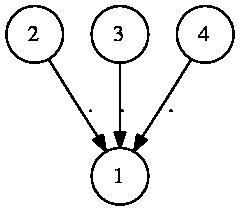
\includegraphics[height=3cm,keepaspectratio=true]{hasse.jpg}   }

 

\subsection{\textcolor{Chapter }{BranchingSubgroup}}
\logpage{[ 7, 2, 22 ]}\nobreak
\hyperdef{L}{X7A874A107D4944E1}{}
{\noindent\textcolor{FuncColor}{$\triangleright$\ \ \texttt{BranchingSubgroup({\mdseries\slshape g})\index{BranchingSubgroup@\texttt{BranchingSubgroup}}
\label{BranchingSubgroup}
}\hfill{\scriptsize (operation)}}\\
\textbf{\indent Returns:\ }
A branching subgroup of \mbox{\texttt{\mdseries\slshape g}}.



 This function searches for a subgroup $k$ of \mbox{\texttt{\mdseries\slshape g}}, such that $k$ contains $k \times \cdots \times k$. 

 It searches for elements in larger and larger balls in \mbox{\texttt{\mdseries\slshape g}}, calling \texttt{FindBranchingSubgroup} (\ref{FindBranchingSubgroup}). 
\begin{Verbatim}[commandchars=!@|,fontsize=\small,frame=single,label=Example]
  !gapprompt@gap>| !gapinput@K := BranchingSubgroup(GrigorchukGroup);|
  <self-similar group over [ 1 .. 2 ] with 9 generators>
  !gapprompt@gap>| !gapinput@IsBranchingSubgroup(K);|
  true
  !gapprompt@gap>| !gapinput@IsBranched(GrigorchukGroup);|
  true
  !gapprompt@gap>| !gapinput@Index(GrigorchukGroup,K);|
  16
\end{Verbatim}
 }

 

\subsection{\textcolor{Chapter }{FindBranchingSubgroup}}
\logpage{[ 7, 2, 23 ]}\nobreak
\hyperdef{L}{X78ADACCD8586D3C7}{}
{\noindent\textcolor{FuncColor}{$\triangleright$\ \ \texttt{FindBranchingSubgroup({\mdseries\slshape g, l, r})\index{FindBranchingSubgroup@\texttt{FindBranchingSubgroup}}
\label{FindBranchingSubgroup}
}\hfill{\scriptsize (operation)}}\\
\textbf{\indent Returns:\ }
A branching subgroup of \mbox{\texttt{\mdseries\slshape g}}.



 This function searches for a subgroup $k$ of \mbox{\texttt{\mdseries\slshape g}}, such that $k$ contains $k \times \cdots \times k$. 

 The second argument \mbox{\texttt{\mdseries\slshape l}} specifies the level at which branching must occur; i.e. asks to search for a
subgroup $k$ such that \mbox{\texttt{\mdseries\slshape g}} contains $k^{d^l}$ where $d$ is the size of the alphabet. If \texttt{l=infinity}, the resulting $k$ will be a regularly branched subgroup. 

 The third argument \mbox{\texttt{\mdseries\slshape r}} specifies the radius to explore in \mbox{\texttt{\mdseries\slshape g}} and all branching subgroups at levels smaller than \mbox{\texttt{\mdseries\slshape l}} for elements with all level-1 states trivial except one. 
\begin{Verbatim}[commandchars=!@|,fontsize=\small,frame=single,label=Example]
  !gapprompt@gap>| !gapinput@FindBranchingSubgroup(GrigorchukGroup,1,4);|
  <self-similar group over [ 1 .. 2 ] with 8 generators>
  !gapprompt@gap>| !gapinput@Index(GrigorchukGroup,last);|
  8
  !gapprompt@gap>| !gapinput@FindBranchingSubgroup(GrigorchukGroup,2,4);|
  <self-similar group over [ 1 .. 2 ] with 6 generators>
  !gapprompt@gap>| !gapinput@Index(GrigorchukGroup,last);|
  16
  !gapprompt@gap>| !gapinput@FindBranchingSubgroup(GrigorchukGroup,3,4);|
  <self-similar group over [ 1 .. 2 ] with 9 generators>
  !gapprompt@gap>| !gapinput@Index(GrigorchukGroup,last);|
  16
\end{Verbatim}
 }

 

\subsection{\textcolor{Chapter }{IsBranched (FR group)}}
\logpage{[ 7, 2, 24 ]}\nobreak
\hyperdef{L}{X832D98E47ACA099C}{}
{\noindent\textcolor{FuncColor}{$\triangleright$\ \ \texttt{IsBranched({\mdseries\slshape g})\index{IsBranched@\texttt{IsBranched}!FR group}
\label{IsBranched:FR group}
}\hfill{\scriptsize (property)}}\\
\textbf{\indent Returns:\ }
\texttt{true} if \mbox{\texttt{\mdseries\slshape g}} has a finite-index branching subgroup.



 This function returns \texttt{true} if \mbox{\texttt{\mdseries\slshape g}} has a finite-index subgroup $k$, such that $k$ contains $k \times \cdots \times k$. 
\begin{Verbatim}[commandchars=@|F,fontsize=\small,frame=single,label=Example]
  <Example><![CDATA[
  @gapprompt|gap>F @gapinput|K := BranchingSubgroup(GrigorchukGroup);F
  <self-similar group over [ 1 .. 2 ] with 9 generators>
  @gapprompt|gap>F @gapinput|IsBranchingSubgroup(K);F
  true
  @gapprompt|gap>F @gapinput|IsBranched(GrigorchukGroup);F
  true
  @gapprompt|gap>F @gapinput|Index(GrigorchukGroup,K);F
  16
\end{Verbatim}
 }

 

\subsection{\textcolor{Chapter }{IsBranchingSubgroup (FR semigroup)}}
\logpage{[ 7, 2, 25 ]}\nobreak
\hyperdef{L}{X7A905CE87B49213F}{}
{\noindent\textcolor{FuncColor}{$\triangleright$\ \ \texttt{IsBranchingSubgroup({\mdseries\slshape k})\index{IsBranchingSubgroup@\texttt{IsBranchingSubgroup}!FR semigroup}
\label{IsBranchingSubgroup:FR semigroup}
}\hfill{\scriptsize (property)}}\\
\textbf{\indent Returns:\ }
\texttt{true} if \mbox{\texttt{\mdseries\slshape k}} is a branching subgroup.



 This function returns \texttt{true} if \mbox{\texttt{\mdseries\slshape k}} contains $k \times \cdots \times k$. 
\begin{Verbatim}[commandchars=!@|,fontsize=\small,frame=single,label=Example]
  !gapprompt@gap>| !gapinput@K := BranchingSubgroup(GrigorchukGroup);|
  <self-similar group over [ 1 .. 2 ] with 9 generators>
  !gapprompt@gap>| !gapinput@IsBranchingSubgroup(K);|
  true
  !gapprompt@gap>| !gapinput@IsBranched(GrigorchukGroup);|
  true
  !gapprompt@gap>| !gapinput@Index(GrigorchukGroup,K);|
  16
\end{Verbatim}
 }

 

\subsection{\textcolor{Chapter }{BranchStructure}}
\logpage{[ 7, 2, 26 ]}\nobreak
\hyperdef{L}{X8404ECA782F2521A}{}
{\noindent\textcolor{FuncColor}{$\triangleright$\ \ \texttt{BranchStructure({\mdseries\slshape G})\index{BranchStructure@\texttt{BranchStructure}}
\label{BranchStructure}
}\hfill{\scriptsize (attribute)}}\\
\textbf{\indent Returns:\ }
A record describing the branching of \mbox{\texttt{\mdseries\slshape G}}.



 This function constructs a record with fields \texttt{group,quo,set,top,wreath,epi} giving respectively a group isomorphic to \texttt{G/K}, the quotient map from \texttt{G} to it, the alphabet of \texttt{G}, the group of permutations of the alphabet, the wreath product of \texttt{group} with its top permutations, and an epimorphism from a subgroup of \texttt{wreath} to \texttt{group}. 

 This information is used as essential data on the branch group, and are used
to construct e.g. its Zeta function. }

 

\subsection{\textcolor{Chapter }{TopVertexTransformations}}
\logpage{[ 7, 2, 27 ]}\nobreak
\hyperdef{L}{X8749E0797A99F531}{}
{\noindent\textcolor{FuncColor}{$\triangleright$\ \ \texttt{TopVertexTransformations({\mdseries\slshape g})\index{TopVertexTransformations@\texttt{TopVertexTransformations}}
\label{TopVertexTransformations}
}\hfill{\scriptsize (attribute)}}\\
\textbf{\indent Returns:\ }
The transformations at the root under the action of \mbox{\texttt{\mdseries\slshape g}}.



 This function returns the permutation group, or the transformation
group/semigroup/monoid, of all activities of all elements under the root
vertex of the tree on which \mbox{\texttt{\mdseries\slshape g}} acts. 

 It is a synonym for \texttt{PermGroup(g,1)} or \texttt{TransMonoid(g,1)} or \texttt{TransSemigroup(g,1)}. 
\begin{Verbatim}[commandchars=!@|,fontsize=\small,frame=single,label=Example]
  !gapprompt@gap>| !gapinput@TopVertexTransformations(GrigorchukGroup);|
  Group([ (), (1,2) ])
  !gapprompt@gap>| !gapinput@IsTransitive(last,AlphabetOfFRSemigroup(GrigorchukGroup));|
  true
  !gapprompt@gap>| !gapinput@TopVertexTransformations(FullSCMonoid([1..3]));|
  <monoid with 3 generators>
  !gapprompt@gap>| !gapinput@Size(last);|
  27
\end{Verbatim}
 }

 

\subsection{\textcolor{Chapter }{VertexTransformations (FR semigroup)}}
\logpage{[ 7, 2, 28 ]}\nobreak
\hyperdef{L}{X7C56C90086070A2E}{}
{\noindent\textcolor{FuncColor}{$\triangleright$\ \ \texttt{VertexTransformations({\mdseries\slshape g})\index{VertexTransformations@\texttt{VertexTransformations}!FR semigroup}
\label{VertexTransformations:FR semigroup}
}\hfill{\scriptsize (attribute)}}\\
\textbf{\indent Returns:\ }
The transformations at all vertices under the action of \mbox{\texttt{\mdseries\slshape g}}.



 This function returns the permutation group, or the transformation
group/monoid/semigroup, of all activities of all elements under all vertices
of the tree on which \mbox{\texttt{\mdseries\slshape g}} acts. 

 This is the smallest group/monoid/semigroup \texttt{P} such that \mbox{\texttt{\mdseries\slshape g}} is a subset of \texttt{FullSCGroup(AlphabetOfFRSemigroup(g),P)} or \texttt{FullSCMonoid(AlphabetOfFRSemigroup(g),P)} or \texttt{FullSCSemigroup(AlphabetOfFRSemigroup(g),P)}. 
\begin{Verbatim}[commandchars=!@|,fontsize=\small,frame=single,label=Example]
  !gapprompt@gap>| !gapinput@VertexTransformations(GuptaSidkiGroup);|
  Group([ (), (1,2,3), (1,3,2) ])
  !gapprompt@gap>| !gapinput@TopVertexTransformations(Group(GuptaSidkiGroup.2));|
  Group(())
  !gapprompt@gap>| !gapinput@VertexTransformations(Group(GuptaSidkiGroup.2));|
  Group([ (), (1,2,3), (1,3,2) ])
\end{Verbatim}
 }

 

\subsection{\textcolor{Chapter }{VirtualEndomorphism}}
\logpage{[ 7, 2, 29 ]}\nobreak
\hyperdef{L}{X7DF2D9838625CDED}{}
{\noindent\textcolor{FuncColor}{$\triangleright$\ \ \texttt{VirtualEndomorphism({\mdseries\slshape g/m, v})\index{VirtualEndomorphism@\texttt{VirtualEndomorphism}}
\label{VirtualEndomorphism}
}\hfill{\scriptsize (operation)}}\\
\textbf{\indent Returns:\ }
The virtual endomorphism at vertex \mbox{\texttt{\mdseries\slshape v}}.



 This function returns the homomorphism from \texttt{Stabilizer(g,v)} to \mbox{\texttt{\mdseries\slshape g}}, defined by computing the state at \mbox{\texttt{\mdseries\slshape v}}. It is loosely speaking an inverse of \texttt{FRGroupByVirtualEndomorphism} (\ref{FRGroupByVirtualEndomorphism}). 

 The first argument \mbox{\texttt{\mdseries\slshape m}} may also be an FR machine. 
\begin{Verbatim}[commandchars=!@|,fontsize=\small,frame=single,label=Example]
  !gapprompt@gap>| !gapinput@A := SCGroup(MealyMachine([[2,1],[2,2]],[(1,2),()]));|
  <self-similar group over [ 1 .. 2 ] with 1 generator>
  !gapprompt@gap>| !gapinput@f := VirtualEndomorphism(A,1);|
  MappingByFunction( <self-similar group over [ 1 .. 2 ] with
  1 generator>, <self-similar group over [ 1 .. 2 ] with
  1 generator>, function( g ) ... end )
  !gapprompt@gap>| !gapinput@((A.1)^2)^f=A.1;|
  true
  !gapprompt@gap>| !gapinput@B := FRGroupByVirtualEndomorphism(f);|
  <self-similar group over [ 1 .. 2 ] with 1 generator>
  !gapprompt@gap>| !gapinput@A=B;|
  true
\end{Verbatim}
 }

 

\subsection{\textcolor{Chapter }{EpimorphismFromFpGroup}}
\logpage{[ 7, 2, 30 ]}\nobreak
\hyperdef{L}{X7C81CB1C7F0D7A90}{}
{\noindent\textcolor{FuncColor}{$\triangleright$\ \ \texttt{EpimorphismFromFpGroup({\mdseries\slshape g, l})\index{EpimorphismFromFpGroup@\texttt{EpimorphismFromFpGroup}}
\label{EpimorphismFromFpGroup}
}\hfill{\scriptsize (operation)}}\\
\textbf{\indent Returns:\ }
An epimorphism from a finitely presented group to \mbox{\texttt{\mdseries\slshape g}}.



 For some examples of self-similar groups, a recursive presentation of the
group is coded into \textsf{FR}, and an approximate presentation is returned by this command, together with a
map onto the group \mbox{\texttt{\mdseries\slshape g}}. The argument \mbox{\texttt{\mdseries\slshape l}} roughly means the number of iterates of an endomorphism were applied to a
finite set of relators. An isomorphic group would be obtained by setting \texttt{l=infinity}; for that purpose, see \texttt{IsomorphismSubgroupFpGroup} (\ref{IsomorphismSubgroupFpGroup}). 

 Preimages can be computed, with \texttt{PreImagesRepresentative}. They are usually reasonably short words, though by no means guaranteed to be
of minimal length. 

 Currently this command is implemented through an ad hoc method for \texttt{BinaryKneadingGroup} (\ref{BinaryKneadingGroup}), \texttt{GrigorchukGroup} (\ref{GrigorchukGroup}) and \texttt{GrigorchukOverGroup} (\ref{GrigorchukOverGroup}). 
\begin{Verbatim}[commandchars=!@|,fontsize=\small,frame=single,label=Example]
  !gapprompt@gap>| !gapinput@f := EpimorphismFromFpGroup(GrigorchukGroup,1);|
  MappingByFunction( <fp group on the generators
  [ a, b, c, d ]>, GrigorchukGroup, function( w ) ... end )
  4 gap> RelatorsOfFpGroup(Source(f));
  [ a^2, b^2, c^2, d^2, b*c*d, a*d*a*d*a*d*a*d, a^-1*c*a*c*a^-1*c*a*c*a^-1*c*a*c*a^
      -1*c*a*c, a^-1*c^-1*a*b*a^-1*c*a*b*a^-1*c^-1*a*b*a^-1*c*a*b*a^-1*c^-1*a*b*a^-1*
      c*a*b*a^-1*c^-1*a*b*a^-1*c*a*b, a*d*a*c*a*c*a*d*a*c*a*c*a*d*a*c*a*c*a*d*a*c*a*c,
    a^-1*c*a*c*a^-1*c*a*b*a^-1*c*a*b*a^-1*c*a*c*a^-1*c*a*b*a^-1*c*a*b*a^-1*c*a*c*a^
      -1*c*a*b*a^-1*c*a*b*a^-1*c*a*c*a^-1*c*a*b*a^-1*c*a*b ]
  !gapprompt@gap>| !gapinput@PreImagesRepresentative(f,Comm(GrigorchukGroup.1,GrigorchukGroup.2));|
  a*c*a*d*a*d*a*c
  !gapprompt@gap>| !gapinput@Source(f).4^f=GrigorchukGroup.4;|
  true
\end{Verbatim}
 }

 

\subsection{\textcolor{Chapter }{IsomorphismSubgroupFpGroup}}
\logpage{[ 7, 2, 31 ]}\nobreak
\hyperdef{L}{X8740656382656D63}{}
{\noindent\textcolor{FuncColor}{$\triangleright$\ \ \texttt{IsomorphismSubgroupFpGroup({\mdseries\slshape g})\index{IsomorphismSubgroupFpGroup@\texttt{IsomorphismSubgroupFpGroup}}
\label{IsomorphismSubgroupFpGroup}
}\hfill{\scriptsize (operation)}}\\
\noindent\textcolor{FuncColor}{$\triangleright$\ \ \texttt{AsSubgroupFpGroup({\mdseries\slshape g})\index{AsSubgroupFpGroup@\texttt{AsSubgroupFpGroup}}
\label{AsSubgroupFpGroup}
}\hfill{\scriptsize (operation)}}\\
\noindent\textcolor{FuncColor}{$\triangleright$\ \ \texttt{IsomorphismLpGroup({\mdseries\slshape g})\index{IsomorphismLpGroup@\texttt{IsomorphismLpGroup}}
\label{IsomorphismLpGroup}
}\hfill{\scriptsize (operation)}}\\
\noindent\textcolor{FuncColor}{$\triangleright$\ \ \texttt{AsLpGroup({\mdseries\slshape g})\index{AsLpGroup@\texttt{AsLpGroup}}
\label{AsLpGroup}
}\hfill{\scriptsize (operation)}}\\
\textbf{\indent Returns:\ }
An isomorphism to a subgroup of a finitely presented group, or an L-presented
group.



 For some examples of self-similar groups, a recursive presentation of the
group is coded into \textsf{FR}, and is returned by this command. The group \mbox{\texttt{\mdseries\slshape g}} itself sits as a subgroup of a finitely presented group. To obtain a finitely
presented group approximating \mbox{\texttt{\mdseries\slshape g}}, see \texttt{EpimorphismFromFpGroup} (\ref{EpimorphismFromFpGroup}). PreImages can also be computed; it is usually better to use \texttt{PreImageElm}, since the word problem may not be solvable by \textsf{GAP} in the f.p. group. 

 Currently this command is implemented through an ad hoc method for \texttt{BinaryKneadingGroup} (\ref{BinaryKneadingGroup}), \texttt{GrigorchukGroup} (\ref{GrigorchukGroup}), \texttt{GrigorchukOverGroup} (\ref{GrigorchukOverGroup}), generalized \texttt{GuptaSidkiGroups} (\ref{GuptaSidkiGroups}) and generalized \texttt{FabrykowskiGuptaGroups} (\ref{FabrykowskiGuptaGroups}). 

 The second form returns an isomorphism to an L-presented group (see \cite{MR2009317} and \cite{MR2483125}. It requires the package \textsf{NQL}. 
\begin{Verbatim}[commandchars=!@|,fontsize=\small,frame=single,label=Example]
  !gapprompt@gap>| !gapinput@f := IsomorphismSubgroupFpGroup(BasilicaGroup);|
  MappingByFunction( BasilicaGroup, Group([ a^-1, a*t^-1*a^-1*t*a^-1
   ]), function( g ) ... end, function( w ) ... end )
  !gapprompt@gap>| !gapinput@Range(f);|
  Group([ a^-1, a*t^-1*a^-1*t*a^-1 ])
  !gapprompt@gap>| !gapinput@c := Comm(BasilicaGroup.1,BasilicaGroup.2);|
  <Mealy element on alphabet [ 1, 2 ] with 9 states, initial state 1>
  !gapprompt@gap>| !gapinput@c^f;|
  t^-2*a*t^-1*a*t*a^-2*t*a*t^-2*a*t^-1*a*t*a^-1*t*a*t^-1*a*t^-2*
  a^-1*t*a*t^-1*a*t^-1*a^-1*t*a^-1*t^5*a*t^-1*a^-1*t*a^-1
  !gapprompt@gap>| !gapinput@PreImageElm(f,last);|
  <Mealy element on alphabet [ 1, 2 ] with 9 states, initial state 1>
  !gapprompt@gap>| !gapinput@last=c;|
  true
\end{Verbatim}
 }

 }

 
\section{\textcolor{Chapter }{Properties for infinite groups}}\logpage{[ 7, 3, 0 ]}
\hyperdef{L}{X7E8485A081EBB3AA}{}
{
 

\subsection{\textcolor{Chapter }{IsTorsionGroup}}
\logpage{[ 7, 3, 1 ]}\nobreak
\hyperdef{L}{X840ED7D279ECAB7F}{}
{\noindent\textcolor{FuncColor}{$\triangleright$\ \ \texttt{IsTorsionGroup({\mdseries\slshape g})\index{IsTorsionGroup@\texttt{IsTorsionGroup}}
\label{IsTorsionGroup}
}\hfill{\scriptsize (property)}}\\
\textbf{\indent Returns:\ }
\texttt{true} if \mbox{\texttt{\mdseries\slshape g}} is a torsion group.



 This function returns \texttt{true} if \mbox{\texttt{\mdseries\slshape g}} is a torsion group, i.e. if every element in \mbox{\texttt{\mdseries\slshape g}} has finite order; and \texttt{false} if \mbox{\texttt{\mdseries\slshape g}} contains an element of infinite order. 

 This method is quite rudimentary, and is not guaranteed to terminate. At the
minimum, \mbox{\texttt{\mdseries\slshape g}} should be a group in which \texttt{Order()} succeeds in computing element orders; e.g. a bounded group in Mealy machine
format. 
\begin{Verbatim}[commandchars=!@|,fontsize=\small,frame=single,label=Example]
  !gapprompt@gap>| !gapinput@Dinfinity := FRGroup("a=(1,2)","b=<a,b>":IsMealyElement);|
  <self-similar group over [ 1 .. 2 ] with 2 generators>
  !gapprompt@gap>| !gapinput@IsTorsionGroup(Dinfinity);|
  false
  !gapprompt@gap>| !gapinput@IsTorsionGroup(GrigorchukGroup); IsTorsionGroup(GuptaSidkiGroup);|
  true
  true
  !gapprompt@gap>| !gapinput@IsTorsionGroup(FabrykowskiGuptaGroup);|
  false
\end{Verbatim}
 }

 

\subsection{\textcolor{Chapter }{IsTorsionFreeGroup}}
\logpage{[ 7, 3, 2 ]}\nobreak
\hyperdef{L}{X7914F2D68077F503}{}
{\noindent\textcolor{FuncColor}{$\triangleright$\ \ \texttt{IsTorsionFreeGroup({\mdseries\slshape g})\index{IsTorsionFreeGroup@\texttt{IsTorsionFreeGroup}}
\label{IsTorsionFreeGroup}
}\hfill{\scriptsize (property)}}\\
\textbf{\indent Returns:\ }
\texttt{true} if \mbox{\texttt{\mdseries\slshape g}} is a torsion-free group.



 This function returns \texttt{true} if \mbox{\texttt{\mdseries\slshape g}} is a torsion-free group, i.e. if no element in \mbox{\texttt{\mdseries\slshape g}} has finite order; and \texttt{false} if \mbox{\texttt{\mdseries\slshape g}} contains an element of finite order. 

 This method is quite rudimentary, and is not guaranteed to terminate. At the
minimum, \mbox{\texttt{\mdseries\slshape g}} should be a group in which \texttt{Order()} succeeds in computing element orders; e.g. a bounded group in Mealy machine
format. 
\begin{Verbatim}[commandchars=!@|,fontsize=\small,frame=single,label=Example]
  !gapprompt@gap>| !gapinput@Dinfinity := FRGroup("a=(1,2)","b=<a,b>":IsMealyElement);|
  <self-similar group over [ 1 .. 2 ] with 2 generators>
  !gapprompt@gap>| !gapinput@IsTorsionFreeGroup(Dinfinity);|
  false
  !gapprompt@gap>| !gapinput@IsTorsionFreeGroup(BasilicaGroup);|
  true
\end{Verbatim}
 }

 

\subsection{\textcolor{Chapter }{IsAmenableGroup}}
\logpage{[ 7, 3, 3 ]}\nobreak
\hyperdef{L}{X87E93FFC820ED40E}{}
{\noindent\textcolor{FuncColor}{$\triangleright$\ \ \texttt{IsAmenableGroup({\mdseries\slshape g})\index{IsAmenableGroup@\texttt{IsAmenableGroup}}
\label{IsAmenableGroup}
}\hfill{\scriptsize (property)}}\\
\textbf{\indent Returns:\ }
\texttt{true} if \mbox{\texttt{\mdseries\slshape g}} is an amenable group.



 Amenable groups, introduced by von Neumann \cite{vneumann}, are those groups that admit a finitely additive, translation-invariant
measure. 
\begin{Verbatim}[commandchars=!@|,fontsize=\small,frame=single,label=Example]
  !gapprompt@gap>| !gapinput@IsAmenableGroup(FreeGroup(2));|
  false
  !gapprompt@gap>| !gapinput@IsAmenableGroup(BasilicaGroup);|
  true
\end{Verbatim}
 }

 

\subsection{\textcolor{Chapter }{IsVirtuallySimpleGroup}}
\logpage{[ 7, 3, 4 ]}\nobreak
\hyperdef{L}{X873C0A7C8422C0C9}{}
{\noindent\textcolor{FuncColor}{$\triangleright$\ \ \texttt{IsVirtuallySimpleGroup({\mdseries\slshape g})\index{IsVirtuallySimpleGroup@\texttt{IsVirtuallySimpleGroup}}
\label{IsVirtuallySimpleGroup}
}\hfill{\scriptsize (property)}}\\
\noindent\textcolor{FuncColor}{$\triangleright$\ \ \texttt{LambdaElementVHGroup({\mdseries\slshape g})\index{LambdaElementVHGroup@\texttt{LambdaElementVHGroup}}
\label{LambdaElementVHGroup}
}\hfill{\scriptsize (attribute)}}\\
\textbf{\indent Returns:\ }
\texttt{true} if \mbox{\texttt{\mdseries\slshape g}} admits a finite-index simple subgroup.



 This function attempts to prove that the VH group \mbox{\texttt{\mdseries\slshape g}} admits a finite-index simple subgroup. 

 It is based on the following test: let \texttt{D} be a direction (vertical or horizontal) such that the corresponding action is
infinitely transitive (see \texttt{IsInfinitelyTransitive} (\ref{IsInfinitelyTransitive})). If the corresponding subgroup of \mbox{\texttt{\mdseries\slshape g}} contains a non-trivial element $\lambda$ that acts trivially in the corresponding action, then every normal subgroup
contains $\lambda$. It then remains to check that the normal closure of $\lambda$ has finite index. This element $\lambda$ is then stored as the attribute \texttt{LambdaElementVHGroup(g)}. 

 The current implementation is based on results in \cite{MR1839488} and \cite{MR1839489}, and does not work for the Rattaggi examples (see \texttt{RattaggiGroup} (\ref{RattaggiGroup})). }

 

\subsection{\textcolor{Chapter }{IsResiduallyFinite}}
\logpage{[ 7, 3, 5 ]}\nobreak
\hyperdef{L}{X79A3A0CF82B6F089}{}
{\noindent\textcolor{FuncColor}{$\triangleright$\ \ \texttt{IsResiduallyFinite({\mdseries\slshape obj})\index{IsResiduallyFinite@\texttt{IsResiduallyFinite}}
\label{IsResiduallyFinite}
}\hfill{\scriptsize (property)}}\\
\textbf{\indent Returns:\ }
\texttt{true} if \mbox{\texttt{\mdseries\slshape obj}} is residually finite.



 An object is \emph{residually finite} if it can be approximated arbitrarily well by finite quotients; i.e. if for
every $g\neq h\in X$ there exists a finite quotient $\pi:X\to Q$ such that $g^\pi\neq h^\pi$. 
\begin{Verbatim}[commandchars=!@|,fontsize=\small,frame=single,label=Example]
  !gapprompt@gap>| !gapinput@IsResiduallyFinite(FreeGroup(2));|
  true
  !gapprompt@gap>| !gapinput@IsResiduallyFinite(BasilicaGroup);|
  true
\end{Verbatim}
 }

 

\subsection{\textcolor{Chapter }{IsSQUniversal}}
\logpage{[ 7, 3, 6 ]}\nobreak
\hyperdef{L}{X86E1182E7EEFAADB}{}
{\noindent\textcolor{FuncColor}{$\triangleright$\ \ \texttt{IsSQUniversal({\mdseries\slshape obj})\index{IsSQUniversal@\texttt{IsSQUniversal}}
\label{IsSQUniversal}
}\hfill{\scriptsize (property)}}\\
\textbf{\indent Returns:\ }
\texttt{true} if \mbox{\texttt{\mdseries\slshape obj}} is SQ-universal.



 An object \mbox{\texttt{\mdseries\slshape obj}} is \emph{SQ-universal} if every countable object of the same category as \mbox{\texttt{\mdseries\slshape obj}} is a subobject of a quotient of \mbox{\texttt{\mdseries\slshape obj}}. 
\begin{Verbatim}[commandchars=!@|,fontsize=\small,frame=single,label=Example]
  !gapprompt@gap>| !gapinput@IsSQUniversal(FreeGroup(2));|
  true
\end{Verbatim}
 }

 

\subsection{\textcolor{Chapter }{IsJustInfinite}}
\logpage{[ 7, 3, 7 ]}\nobreak
\hyperdef{L}{X7FDAEAFF78A5E7D2}{}
{\noindent\textcolor{FuncColor}{$\triangleright$\ \ \texttt{IsJustInfinite({\mdseries\slshape obj})\index{IsJustInfinite@\texttt{IsJustInfinite}}
\label{IsJustInfinite}
}\hfill{\scriptsize (property)}}\\
\textbf{\indent Returns:\ }
\texttt{true} if \mbox{\texttt{\mdseries\slshape obj}} is just-infinite.



 An object \mbox{\texttt{\mdseries\slshape obj}} is \emph{just-infinite} if \mbox{\texttt{\mdseries\slshape obj}} is infinite, but every quotient of \mbox{\texttt{\mdseries\slshape obj}} is finite. 
\begin{Verbatim}[commandchars=!@|,fontsize=\small,frame=single,label=Example]
  !gapprompt@gap>| !gapinput@IsJustInfinite(FreeGroup(2));|
  false
  !gapprompt@gap>| !gapinput@IsJustInfinite(FreeGroup(1));|
  true
  !gapprompt@gap>| !gapinput@IsJustInfinite(GrigorchukGroup); time|
  true
  8284
\end{Verbatim}
 }

 }

 }

 
\chapter{\textcolor{Chapter }{Algebras}}\label{algebras}
\logpage{[ 8, 0, 0 ]}
\hyperdef{L}{X7DDBF6F47A2E021C}{}
{
 Self-similar algebras and algebras with one (below \emph{FR algebras}) are simply algebras [with one] whose elements are linear FR machines. They
naturally act on the alphabet of their elements, which is a vector space. 

 Elements may be added, subtracted and multiplied. They can be vector or
algebra linear elements; the vector elements are in general preferable, for
efficiency reasons. 

 Finite-dimensional approximations of self-similar algebras can be computed;
they are given as matrix algebras. 
\section{\textcolor{Chapter }{Creators for FR algebras}}\logpage{[ 8, 1, 0 ]}
\hyperdef{L}{X842EE9427C63F92E}{}
{
 The most straightforward creation method for FR algebras is \texttt{Algebra()}, applied with linear FR elements as arguments. There are shortcuts to this
somewhat tedious method: 

\subsection{\textcolor{Chapter }{FRAlgebra}}
\logpage{[ 8, 1, 1 ]}\nobreak
\hyperdef{L}{X812FEA6778152E49}{}
{\noindent\textcolor{FuncColor}{$\triangleright$\ \ \texttt{FRAlgebra({\mdseries\slshape ring, \texttt{\symbol{123}}definition, \texttt{\symbol{125}}})\index{FRAlgebra@\texttt{FRAlgebra}}
\label{FRAlgebra}
}\hfill{\scriptsize (operation)}}\\
\noindent\textcolor{FuncColor}{$\triangleright$\ \ \texttt{FRAlgebraWithOne({\mdseries\slshape ring, \texttt{\symbol{123}}definition, \texttt{\symbol{125}}})\index{FRAlgebraWithOne@\texttt{FRAlgebraWithOne}}
\label{FRAlgebraWithOne}
}\hfill{\scriptsize (operation)}}\\
\textbf{\indent Returns:\ }
A new self-similar algebra [with one].



 This function constructs a new FR algebra [with one], generated by linear FR
elements. It receives as argument any number of strings, each of which
represents a generator of the object to be constructed. 

 \mbox{\texttt{\mdseries\slshape ring}} is the acting domain of the vector space on which the algebra will act. 

 Each \mbox{\texttt{\mdseries\slshape definition}} is of the form \texttt{"name=[[...],...,[...]]"} or of the form \texttt{"name=[[...],...,[...]]:out"}, namely a matrix whose entries are algebraic expressions in the \texttt{names}, possibly using \texttt{0,1}, optionally followed by a scalar. The matrix entries specify the
decomposition of the element being defined, and the optional scalar specifies
the output of that element, by default assumed to be one. 

 The option \texttt{IsVectorElement} asks for the resulting algebra to be generated by vector elements, see example
below. The generators must of course be finite-state. 
\begin{Verbatim}[commandchars=!@|,fontsize=\small,frame=single,label=Example]
  !gapprompt@gap>| !gapinput@m := FRAlgebra(Rationals,"a=[[1,a],[a,0]]");|
  <self-similar algebra on alphabet Rationals^2 with 1 generator>
  !gapprompt@gap>| !gapinput@Display(Activity(m.1,2));|
  [ [  1,  0,  1,  1 ],
    [  0,  1,  1,  0 ],
    [  1,  1,  0,  0 ],
    [  1,  0,  0,  0 ] ]
  !gapprompt@gap>| !gapinput@m2 := FRAlgebra(Rationals,"a=[[1,a],[a,0]]":IsVectorElement);;|
  !gapprompt@gap>| !gapinput@m.1=m2.1;|
  true
\end{Verbatim}
 }

 

\subsection{\textcolor{Chapter }{SCAlgebra}}
\logpage{[ 8, 1, 2 ]}\nobreak
\hyperdef{L}{X844B890F7BF56236}{}
{\noindent\textcolor{FuncColor}{$\triangleright$\ \ \texttt{SCAlgebra({\mdseries\slshape m})\index{SCAlgebra@\texttt{SCAlgebra}}
\label{SCAlgebra}
}\hfill{\scriptsize (operation)}}\\
\noindent\textcolor{FuncColor}{$\triangleright$\ \ \texttt{SCLieAlgebra({\mdseries\slshape m})\index{SCLieAlgebra@\texttt{SCLieAlgebra}}
\label{SCLieAlgebra}
}\hfill{\scriptsize (operation)}}\\
\noindent\textcolor{FuncColor}{$\triangleright$\ \ \texttt{SCAlgebraWithOne({\mdseries\slshape m})\index{SCAlgebraWithOne@\texttt{SCAlgebraWithOne}}
\label{SCAlgebraWithOne}
}\hfill{\scriptsize (operation)}}\\
\noindent\textcolor{FuncColor}{$\triangleright$\ \ \texttt{SCAlgebraNC({\mdseries\slshape m})\index{SCAlgebraNC@\texttt{SCAlgebraNC}}
\label{SCAlgebraNC}
}\hfill{\scriptsize (operation)}}\\
\noindent\textcolor{FuncColor}{$\triangleright$\ \ \texttt{SCAlgebraWithOneNC({\mdseries\slshape m})\index{SCAlgebraWithOneNC@\texttt{SCAlgebraWithOneNC}}
\label{SCAlgebraWithOneNC}
}\hfill{\scriptsize (operation)}}\\
\textbf{\indent Returns:\ }
The state-closed algebra [with one] generated by the machine \mbox{\texttt{\mdseries\slshape m}}.



 This function constructs a new FR algebra [vith one] \texttt{a}, generated by all the states of the FR machine \mbox{\texttt{\mdseries\slshape m}}. There is a bijective correspondence between \texttt{GeneratorsOfFRMachine(m)} and the generators of \texttt{a}, which is accessible via \texttt{Correspondence(a)} (See \texttt{Correspondence} (\ref{Correspondence:FR semigroup})); it is a homomorphism from the stateset of \mbox{\texttt{\mdseries\slshape m}} to \texttt{a}, or a list indicating for each state of \mbox{\texttt{\mdseries\slshape m}} a corresponding generator index in the generators of \texttt{a} (with 0 for identity). 

 In the non-\texttt{NC} forms, redundant (equal, zero or one) states are removed from the generating
set of \texttt{a}. 
\begin{Verbatim}[commandchars=!@|,fontsize=\small,frame=single,label=Example]
  !gapprompt@gap>| !gapinput@a := SCAlgebra(AsLinearMachine(Rationals,I4Machine));|
  <self-similar algebra on alphabet Rationals^2 with 3 generators>
  !gapprompt@gap>| !gapinput@a.1 = AsLinearElement(Rationals,I4Monoid.1);|
  true
\end{Verbatim}
 }

 

\subsection{\textcolor{Chapter }{NucleusOfFRAlgebra}}
\logpage{[ 8, 1, 3 ]}\nobreak
\hyperdef{L}{X7B8330F180BABC43}{}
{\noindent\textcolor{FuncColor}{$\triangleright$\ \ \texttt{NucleusOfFRAlgebra({\mdseries\slshape a})\index{NucleusOfFRAlgebra@\texttt{NucleusOfFRAlgebra}}
\label{NucleusOfFRAlgebra}
}\hfill{\scriptsize (attribute)}}\\
\noindent\textcolor{FuncColor}{$\triangleright$\ \ \texttt{Nucleus({\mdseries\slshape a})\index{Nucleus@\texttt{Nucleus}!FR algebra}
\label{Nucleus:FR algebra}
}\hfill{\scriptsize (operation)}}\\
\textbf{\indent Returns:\ }
The nucleus of the contracting algebra \mbox{\texttt{\mdseries\slshape a}}.



 This function returns the \emph{nucleus} of the contracting algebra \mbox{\texttt{\mdseries\slshape a}}, i.e. the smallest subspace \texttt{N} of \mbox{\texttt{\mdseries\slshape a}} such that the \texttt{LimitStates} (\ref{LimitStates}) of every element of \mbox{\texttt{\mdseries\slshape a}} belong to \texttt{N}. 

 This function returns \texttt{fail} if no such \texttt{N} exists. Usually, it loops forever without being able to decide whether \texttt{N} is finite or infinite. It succeeds precisely when \texttt{IsContracting(g)} succeeds. 
\begin{Verbatim}[commandchars=!@|,fontsize=\small,frame=single,label=Example]
  !gapprompt@gap>| !gapinput@> a := GrigorchukThinnedAlgebra(2);|
  <self-similar algebra-with-one on alphabet GF(2)^2 with 4 generators, of dimension infinity>
  !gapprompt@gap>| !gapinput@NucleusOfFRAlgebra(a);|
  <vector space over GF(2), with 4 generators>
\end{Verbatim}
 }

 

\subsection{\textcolor{Chapter }{BranchingIdeal}}
\logpage{[ 8, 1, 4 ]}\nobreak
\hyperdef{L}{X81D8D0E886C8E143}{}
{\noindent\textcolor{FuncColor}{$\triangleright$\ \ \texttt{BranchingIdeal({\mdseries\slshape A})\index{BranchingIdeal@\texttt{BranchingIdeal}}
\label{BranchingIdeal}
}\hfill{\scriptsize (operation)}}\\
\textbf{\indent Returns:\ }
An ideal $I$ that contains matrices over itself.



 
\begin{Verbatim}[commandchars=!@|,fontsize=\small,frame=single,label=Example]
  !gapprompt@gap>| !gapinput@R := GrigorchukThinnedAlgebra(2);;|
  !gapprompt@gap>| !gapinput@I := BranchingIdeal(R);|
  <two-sided ideal in <self-similar algebra-with-one on alphabet GF(2)^2
   with 4 generators, of dimension infinity>, (3 generators)>
  !gapprompt@gap>| !gapinput@e := EpimorphismMatrixQuotient(R,3);;|
  !gapprompt@gap>| !gapinput@eI := Ideal(Range(e),List(GeneratorsOfIdeal(I),x->x^e));|
  <two-sided ideal in <algebra-with-one of dimension 22 over GF(2)>, (3 generators)>
  !gapprompt@gap>| !gapinput@Dimension(Range(e)/eI);|
  6
\end{Verbatim}
 }

 }

 
\section{\textcolor{Chapter }{Operations for FR algebras}}\logpage{[ 8, 2, 0 ]}
\hyperdef{L}{X7EFB4F2E7E908B9F}{}
{
 

\subsection{\textcolor{Chapter }{MatrixQuotient}}
\logpage{[ 8, 2, 1 ]}\nobreak
\hyperdef{L}{X8115B018871FD364}{}
{\noindent\textcolor{FuncColor}{$\triangleright$\ \ \texttt{MatrixQuotient({\mdseries\slshape a, l})\index{MatrixQuotient@\texttt{MatrixQuotient}}
\label{MatrixQuotient}
}\hfill{\scriptsize (operation)}}\\
\noindent\textcolor{FuncColor}{$\triangleright$\ \ \texttt{EpimorphismMatrixQuotient({\mdseries\slshape a, l})\index{EpimorphismMatrixQuotient@\texttt{EpimorphismMatrixQuotient}}
\label{EpimorphismMatrixQuotient}
}\hfill{\scriptsize (operation)}}\\
\textbf{\indent Returns:\ }
The matrix algebra of \mbox{\texttt{\mdseries\slshape a}}'s action on level \mbox{\texttt{\mdseries\slshape l}}.



 The first function returns the matrix algebra generated by the activities of \mbox{\texttt{\mdseries\slshape a}} on level \mbox{\texttt{\mdseries\slshape l}} (see the examples in \ref{ActivitySparse}). The second functon returns an algebra homomorphism from \mbox{\texttt{\mdseries\slshape a}} to the matrix algebra. 
\begin{Verbatim}[commandchars=!@|,fontsize=\small,frame=single,label=Example]
  !gapprompt@gap>| !gapinput@a := ThinnedAlgebraWithOne(GF(2),GrigorchukGroup);|
  <self-similar algebra-with-one on alphabet GF(2)^2 with 4 generators>
  !gapprompt@gap>| !gapinput@List([0..4],i->Dimension(MatrixQuotient(a,i)));|
  [ 1, 2, 6, 22, 78 ]
\end{Verbatim}
 }

 

\subsection{\textcolor{Chapter }{ThinnedAlgebra}}
\logpage{[ 8, 2, 2 ]}\nobreak
\hyperdef{L}{X8150FC4E84D208C6}{}
{\noindent\textcolor{FuncColor}{$\triangleright$\ \ \texttt{ThinnedAlgebra({\mdseries\slshape r, g})\index{ThinnedAlgebra@\texttt{ThinnedAlgebra}}
\label{ThinnedAlgebra}
}\hfill{\scriptsize (operation)}}\\
\noindent\textcolor{FuncColor}{$\triangleright$\ \ \texttt{ThinnedAlgebraWithOne({\mdseries\slshape r, g})\index{ThinnedAlgebraWithOne@\texttt{ThinnedAlgebraWithOne}}
\label{ThinnedAlgebraWithOne}
}\hfill{\scriptsize (operation)}}\\
\textbf{\indent Returns:\ }
The thinned algebra [with one] associated with \mbox{\texttt{\mdseries\slshape g}}.



 The first function returns the thinned algebra of a FR group/monoid/semigroup \mbox{\texttt{\mdseries\slshape g}}, over the domain \mbox{\texttt{\mdseries\slshape r}}. This is the linear envelope of \mbox{\texttt{\mdseries\slshape g}} in its natural action on sequences. 

 The embedding of \mbox{\texttt{\mdseries\slshape g}} in its thinned algebra is returned by \texttt{Embedding(g,a)}. 
\begin{Verbatim}[commandchars=!@|,fontsize=\small,frame=single,label=Example]
  !gapprompt@gap>| !gapinput@a := ThinnedAlgebraWithOne(GF(2),GrigorchukGroup);|
  <self-similar algebra on alphabet GF(2)^2 with 5 generators>
  !gapprompt@gap>| !gapinput@a.1 = GrigorchukGroup.1^Embedding(GrigorchukGroup,a);|
  true
  !gapprompt@gap>| !gapinput@Dimension(VectorSpace(GF(2),[One(a),a.2,a.3,a.4]));|
  3
\end{Verbatim}
 }

 

\subsection{\textcolor{Chapter }{Nillity}}
\logpage{[ 8, 2, 3 ]}\nobreak
\hyperdef{L}{X8572DCAE7F888DDA}{}
{\noindent\textcolor{FuncColor}{$\triangleright$\ \ \texttt{Nillity({\mdseries\slshape x})\index{Nillity@\texttt{Nillity}}
\label{Nillity}
}\hfill{\scriptsize (attribute)}}\\
\noindent\textcolor{FuncColor}{$\triangleright$\ \ \texttt{IsNilElement({\mdseries\slshape x})\index{IsNilElement@\texttt{IsNilElement}}
\label{IsNilElement}
}\hfill{\scriptsize (property)}}\\
\textbf{\indent Returns:\ }
The smallest \texttt{n} such that $x^n=0$.



 The first command computes the nillity of \mbox{\texttt{\mdseries\slshape x}}, i.e. the smallest \texttt{n} such that $x^n=0$. The command is not guaranteed to terminate. 

 The second command returns whether \mbox{\texttt{\mdseries\slshape x}} is nil, that is, whether its nillity is finite. }

 

\subsection{\textcolor{Chapter }{DegreeOfHomogeneousElement}}
\logpage{[ 8, 2, 4 ]}\nobreak
\hyperdef{L}{X85163F29824C944D}{}
{\noindent\textcolor{FuncColor}{$\triangleright$\ \ \texttt{DegreeOfHomogeneousElement({\mdseries\slshape x})\index{DegreeOfHomogeneousElement@\texttt{DegreeOfHomogeneousElement}}
\label{DegreeOfHomogeneousElement}
}\hfill{\scriptsize (attribute)}}\\
\noindent\textcolor{FuncColor}{$\triangleright$\ \ \texttt{IsHomogeneousElement({\mdseries\slshape x})\index{IsHomogeneousElement@\texttt{IsHomogeneousElement}}
\label{IsHomogeneousElement}
}\hfill{\scriptsize (property)}}\\
\textbf{\indent Returns:\ }
The degree of \mbox{\texttt{\mdseries\slshape x}} in its parent.



 If \mbox{\texttt{\mdseries\slshape x}} belongs to a graded algebra \texttt{A}, then the second command returns whether \mbox{\texttt{\mdseries\slshape x}} belongs to a homogeneous component of \texttt{Grading(A)}, and the first command returns the degree of that component (or \texttt{fail} if no such component exists). }

 }

 }

 
\chapter{\textcolor{Chapter }{Iterated monodromy groups}}\label{img}
\logpage{[ 9, 0, 0 ]}
\hyperdef{L}{X798DE1297EC58F59}{}
{
 Iterated monodromy machines are a special class of group FR machines (see
Section \ref{frmachines}) with attribute \texttt{IMGRelator} (\ref{IMGRelator}). This attribute records a cyclic ordering of the generators of the machine
whose product is trivial. 

 The interpretation is the following: the machine encodes a \emph{Thurston map}, i.e. a post-critically finite topological branched self-covering of the
sphere $S^2$. Generators of the machine correspond to loops in the fundamental group of
the sphere (punctured at post-critical points), that circle once
counter-clockwise around a post-critical point. For more details on the
connection between self-similar groups and Thurston maps, see \cite{MR2162164}. 

 IMG elements are a bit different from group FR elements: while we said a group
FR element is trivial if and only if its action on sequences is trivial, we
say that an IMG element $g$ is trivial if there exists an integer $N$ such that unfolding $N$ times the recursion for $g$ yields only trivial states (as elements of the underlying free group). 
\section{\textcolor{Chapter }{Creators and operations for IMG machines}}\logpage{[ 9, 1, 0 ]}
\hyperdef{L}{X8287B3D98071EBB7}{}
{
 

\subsection{\textcolor{Chapter }{IsIMGMachine}}
\logpage{[ 9, 1, 1 ]}\nobreak
\hyperdef{L}{X851C12AA87B92799}{}
{\noindent\textcolor{FuncColor}{$\triangleright$\ \ \texttt{IsIMGMachine({\mdseries\slshape m})\index{IsIMGMachine@\texttt{IsIMGMachine}}
\label{IsIMGMachine}
}\hfill{\scriptsize (filter)}}\\
\noindent\textcolor{FuncColor}{$\triangleright$\ \ \texttt{IsPolynomialFRMachine({\mdseries\slshape m})\index{IsPolynomialFRMachine@\texttt{IsPolynomialFRMachine}}
\label{IsPolynomialFRMachine}
}\hfill{\scriptsize (filter)}}\\
\noindent\textcolor{FuncColor}{$\triangleright$\ \ \texttt{IsPolynomialIMGMachine({\mdseries\slshape m})\index{IsPolynomialIMGMachine@\texttt{IsPolynomialIMGMachine}}
\label{IsPolynomialIMGMachine}
}\hfill{\scriptsize (filter)}}\\


 The categories of \emph{IMG} and \emph{polynomial} machines. IMG machines are group FR machines with an additional element, their
attribute \texttt{IMGRelator} (\ref{IMGRelator}); see \texttt{AsIMGMachine} (\ref{AsIMGMachine}). 

 A polynomial machine is a group FR machine with a distinguished state (which
must be a generator of the stateset), stored as the attribute \texttt{AddingElement} (\ref{AddingElement}); see \texttt{AsPolynomialFRMachine} (\ref{AsPolynomialFRMachine}). If it is normalized, in the sense that the wreath recursion of the adding
element \texttt{a} is \texttt{[[a,1,...,1],[d,1,...,d-1]]}, then the basepoint is assumed to be at $+\infty$; the element \texttt{a} describes a clockwise loop around infinity; the $k$th preimage of the basepoint is at $\exp(2i\pi(k-1)/d)\infty$, for $k=1,\dots,d$; and there is a direct connection from basepoint $k$ to $k+1$ for all $k=1,\dots,d-1$. 

 The last category is the intersection of the first two. }

 

\subsection{\textcolor{Chapter }{IMGMachineNC}}
\logpage{[ 9, 1, 2 ]}\nobreak
\hyperdef{L}{X78D75CDE792449A6}{}
{\noindent\textcolor{FuncColor}{$\triangleright$\ \ \texttt{IMGMachineNC({\mdseries\slshape fam, group, trans, out, rel})\index{IMGMachineNC@\texttt{IMGMachineNC}}
\label{IMGMachineNC}
}\hfill{\scriptsize (operation)}}\\
\textbf{\indent Returns:\ }
An IMG FR machine.



 This function creates, without checking its arguments, a new IMG machine in
family \mbox{\texttt{\mdseries\slshape fam}}, stateset \mbox{\texttt{\mdseries\slshape group}}, with transitions and output \mbox{\texttt{\mdseries\slshape trans,out}}, and IMG relator \mbox{\texttt{\mdseries\slshape rel}}. }

 

\subsection{\textcolor{Chapter }{AsIMGMachine}}
\logpage{[ 9, 1, 3 ]}\nobreak
\hyperdef{L}{X857CD5C587549F1A}{}
{\noindent\textcolor{FuncColor}{$\triangleright$\ \ \texttt{AsIMGMachine({\mdseries\slshape m[, w]})\index{AsIMGMachine@\texttt{AsIMGMachine}}
\label{AsIMGMachine}
}\hfill{\scriptsize (operation)}}\\
\textbf{\indent Returns:\ }
An IMG FR machine.



 This function creates a new IMG FR machine, starting from a group FR machine \mbox{\texttt{\mdseries\slshape m}}. If a state \texttt{w} is specified, and that state defines the trivial FR element, then it is used
as \texttt{IMGRelator} (\ref{IMGRelator}); if the state \texttt{w} is non-trivial, then a new generator \texttt{f} is added to \mbox{\texttt{\mdseries\slshape m}}, equal to the inverse of \texttt{w}; and the IMG relator is chosen to be \texttt{w*f}. Finally, if no relator is specified, and the product (in some ordering) of
the generators is trivial, then that product is used as IMG relator. In other
cases, the method returns \texttt{fail}. 

 Note that IMG elements and FR elements are compared differently (see the
example below); namely, an FR element is trivial precisely when it acts
trivially on sequences. An IMG element is trivial precisely when a finite
number of applications of free cancellation, the IMG relator, and the
decomposition map, result in trivial elements of the underlying free group. 

 A standard FR machine can be recovered from an IMG FR machine by \texttt{AsGroupFRMachine} (\ref{AsGroupFRMachine}), \texttt{AsMonoidFRMachine} (\ref{AsMonoidFRMachine}), and \texttt{AsSemigroupFRMachine} (\ref{AsSemigroupFRMachine}). 
\begin{Verbatim}[commandchars=!@C,fontsize=\small,frame=single,label=Example]
  !gapprompt@gap>C !gapinput@m := UnderlyingFRMachine(BasilicaGroup);C
  <Mealy machine on alphabet [ 1 .. 2 ] with 3 states>
  !gapprompt@gap>C !gapinput@g := AsGroupFRMachine(m);C
  <FR machine with alphabet [ 1 .. 2 ] on Group( [ f1, f2 ] )>
  !gapprompt@gap>C !gapinput@AsIMGMachine(g,Product(GeneratorsOfFRMachine(g)));C
  <FR machine with alphabet [ 1 .. 2 ] on Group( [ f1, f2, t ] )/[ f1*f2*t ]>
  !gapprompt@gap>C !gapinput@Display(last);C
   G  |              1         2
  ----+-----------------+---------+
   f1 |          <id>,2      f2,1
   f2 |          <id>,1      f1,2
    t | f2^-1*f1*f2*t,2   f1^-1,1
  ----+-----------------+---------+
  Relator: f1*f2*t
  !gapprompt@gap>C !gapinput@g := AsGroupFRMachine(GuptaSidkiMachine);C
  <FR machine with alphabet [ 1 .. 3 ] on Group( [ f1, f2 ] )>
  !gapprompt@gap>C !gapinput@m := AsIMGMachine(g,GeneratorsOfFRMachine(g)[1]);C
  <FR machine with alphabet [ 1 .. 3 ] on Group( [ f1, f2, t ] )/[ f1*t ]>
  !gapprompt@gap>C !gapinput@x := FRElement(g,2)^3; IsOne(x);C
  <3|identity ...>
  true
  !gapprompt@gap>C !gapinput@x := FRElement(m,2)^3; IsOne(x);C
  <3#f2^3>
  false
\end{Verbatim}
 }

 

\subsection{\textcolor{Chapter }{IMGRelator}}
\logpage{[ 9, 1, 4 ]}\nobreak
\hyperdef{L}{X7BCE03F2827DAA0A}{}
{\noindent\textcolor{FuncColor}{$\triangleright$\ \ \texttt{IMGRelator({\mdseries\slshape m})\index{IMGRelator@\texttt{IMGRelator}}
\label{IMGRelator}
}\hfill{\scriptsize (attribute)}}\\
\textbf{\indent Returns:\ }
The relator of the IMG FR machine.



 This attribute stores the product of generators that is trivial. In essence,
it records an ordering of the generators whose product is trivial in the
punctured sphere's fundamental group. }

 

\subsection{\textcolor{Chapter }{CleanedIMGMachine}}
\logpage{[ 9, 1, 5 ]}\nobreak
\hyperdef{L}{X8706C13B7D6A1225}{}
{\noindent\textcolor{FuncColor}{$\triangleright$\ \ \texttt{CleanedIMGMachine({\mdseries\slshape m})\index{CleanedIMGMachine@\texttt{CleanedIMGMachine}}
\label{CleanedIMGMachine}
}\hfill{\scriptsize (attribute)}}\\
\textbf{\indent Returns:\ }
A cleaned-up version of \mbox{\texttt{\mdseries\slshape m}}.



 This command attempts to shorten the length of the transitions in \mbox{\texttt{\mdseries\slshape m}}, and ensure (if possible) that the product along every cycle of the states of
a generator is a conjugate of a generator. It returns the new machine. }

 

\subsection{\textcolor{Chapter }{NewSemigroupFRMachine}}
\logpage{[ 9, 1, 6 ]}\nobreak
\hyperdef{L}{X7D4A6996874A3DF3}{}
{\noindent\textcolor{FuncColor}{$\triangleright$\ \ \texttt{NewSemigroupFRMachine({\mdseries\slshape ...})\index{NewSemigroupFRMachine@\texttt{NewSemigroupFRMachine}}
\label{NewSemigroupFRMachine}
}\hfill{\scriptsize (attribute)}}\\
\noindent\textcolor{FuncColor}{$\triangleright$\ \ \texttt{NewMonoidFRMachine({\mdseries\slshape ...})\index{NewMonoidFRMachine@\texttt{NewMonoidFRMachine}}
\label{NewMonoidFRMachine}
}\hfill{\scriptsize (attribute)}}\\
\noindent\textcolor{FuncColor}{$\triangleright$\ \ \texttt{NewGroupFRMachine({\mdseries\slshape ...})\index{NewGroupFRMachine@\texttt{NewGroupFRMachine}}
\label{NewGroupFRMachine}
}\hfill{\scriptsize (attribute)}}\\
\noindent\textcolor{FuncColor}{$\triangleright$\ \ \texttt{NewIMGMachine({\mdseries\slshape ...})\index{NewIMGMachine@\texttt{NewIMGMachine}}
\label{NewIMGMachine}
}\hfill{\scriptsize (attribute)}}\\
\textbf{\indent Returns:\ }
A new FR machine, based on string descriptions.



 This command constructs a new FR or IMG machine, in a format similar to \texttt{FRGroup} (\ref{FRGroup}); namely, the arguments are strings of the form
"gen={\textless}word-1,...,word-d{\textgreater}perm"; each \texttt{word-i} is a word in the generators; and \texttt{perm} is a transformation, either written in disjoint cycle or in images notation. 

Except in the semigroup case, \texttt{word-i} is allowed to be the empty string; and the "{\textless}...{\textgreater}" may
be skipped altogether. In the group or IMG case, each \texttt{word-i} may also contain inverses. 

In the IMG case, an extra final argument is allowed, which is a word in the
generators, and describes the IMG relation. If absent, \textsf{FR} will attempt to find such a relation. 

The following examples construct realizable foldings of the polynomial $z^3+i$, following Cui's arguments. 
\begin{Verbatim}[commandchars=!@|,fontsize=\small,frame=single,label=Example]
  !gapprompt@gap>| !gapinput@fold1 := NewIMGMachine("a=<,,b,,,B>(1,2,3)(4,5,6)","b=<,,b*a/b,,,B*A/B>",|
       "A=<,,b*a,,,B*A>(3,6)","B=(1,6,5,4,3,2)");
  !gapprompt@gap>| !gapinput@<FR machine with alphabet [ 1, 2, 3, 4, 5, 6 ] on Group( [ a, b, A, B ] )/[ a*B*A*b ]>                                |
  !gapprompt@gap>| !gapinput@fold2 := NewIMGMachine("a=<,,b,,,B>(1,2,3)(4,5,6)","b=<,,b*a/b,,,B*A/B>",|
       "A=(1,6)(2,5)(3,4)","B=<B*A,,,b*a,,>(1,4)(2,6)(3,5)");;
  !gapprompt@gap>| !gapinput@RationalFunction(fold1); RationalFunction(fold2);|
  ...
\end{Verbatim}
 }

 

\subsection{\textcolor{Chapter }{AsIMGElement}}
\logpage{[ 9, 1, 7 ]}\nobreak
\hyperdef{L}{X80388DDE7F9B41FD}{}
{\noindent\textcolor{FuncColor}{$\triangleright$\ \ \texttt{AsIMGElement({\mdseries\slshape e})\index{AsIMGElement@\texttt{AsIMGElement}}
\label{AsIMGElement}
}\hfill{\scriptsize (operation)}}\\
\noindent\textcolor{FuncColor}{$\triangleright$\ \ \texttt{IsIMGElement({\mdseries\slshape e})\index{IsIMGElement@\texttt{IsIMGElement}}
\label{IsIMGElement}
}\hfill{\scriptsize (filter)}}\\


 The category of \emph{IMG elements}, namely FR elements of an IMG machine. See \texttt{AsIMGMachine} (\ref{AsIMGMachine}) for details. }

 

\subsection{\textcolor{Chapter }{IsKneadingMachine}}
\logpage{[ 9, 1, 8 ]}\nobreak
\hyperdef{L}{X84C2881D87C1FB74}{}
{\noindent\textcolor{FuncColor}{$\triangleright$\ \ \texttt{IsKneadingMachine({\mdseries\slshape m})\index{IsKneadingMachine@\texttt{IsKneadingMachine}}
\label{IsKneadingMachine}
}\hfill{\scriptsize (property)}}\\
\noindent\textcolor{FuncColor}{$\triangleright$\ \ \texttt{IsPlanarKneadingMachine({\mdseries\slshape m})\index{IsPlanarKneadingMachine@\texttt{IsPlanarKneadingMachine}}
\label{IsPlanarKneadingMachine}
}\hfill{\scriptsize (property)}}\\
\textbf{\indent Returns:\ }
Whether \mbox{\texttt{\mdseries\slshape m}} is a (planar) kneading machine.



 A \emph{kneading machine} is a special kind of Mealy machine, used to describe postcritically finite
complex polynomials. It is a machine such that its set of permutations is
"treelike" (see \cite[{\S}6.7]{MR2162164}) and such that each non-trivial state occurs exactly once among the outputs. 

 Furthermore, this set of permutations is \emph{treelike} if there exists an ordering of the states that their product in that order $t$ is an adding machine; i.e. such that $t$'s activity is a full cycle, and the product of its states along that cycle is
conjugate to $t$. This element $t$ represents the Carath{\a'e}odory loop around infinity. 
\begin{Verbatim}[commandchars=!@A,fontsize=\small,frame=single,label=Example]
  !gapprompt@gap>A !gapinput@M := BinaryKneadingMachine("0");A
  BinaryKneadingMachine("0*")
  !gapprompt@gap>A !gapinput@Display(M);A
     |  1     2
  ---+-----+-----+
   a | c,2   b,1
   b | a,1   c,2
   c | c,1   c,2
  ---+-----+-----+
  !gapprompt@gap>A !gapinput@IsPlanarKneadingMachine(M);A
  true
  !gapprompt@gap>A !gapinput@IsPlanarKneadingMachine(GrigorchukMachine);A
  false
\end{Verbatim}
 }

 

\subsection{\textcolor{Chapter }{AsPolynomialFRMachine}}
\logpage{[ 9, 1, 9 ]}\nobreak
\hyperdef{L}{X8203D69280D4B64C}{}
{\noindent\textcolor{FuncColor}{$\triangleright$\ \ \texttt{AsPolynomialFRMachine({\mdseries\slshape m[, adder]})\index{AsPolynomialFRMachine@\texttt{AsPolynomialFRMachine}}
\label{AsPolynomialFRMachine}
}\hfill{\scriptsize (operation)}}\\
\noindent\textcolor{FuncColor}{$\triangleright$\ \ \texttt{AsPolynomialIMGMachine({\mdseries\slshape m[, adder[, relator]]})\index{AsPolynomialIMGMachine@\texttt{AsPolynomialIMGMachine}}
\label{AsPolynomialIMGMachine}
}\hfill{\scriptsize (operation)}}\\
\textbf{\indent Returns:\ }
A polynomial FR machine.



 The first function creates a new polynomial FR machine, starting from a group
or Mealy machine. A \emph{polynomial} machine is one that has a distinguished adding element, \texttt{AddingElement} (\ref{AddingElement}). 

 If the argument is a Mealy machine, it must be planar (see \texttt{IsPlanarKneadingMachine} (\ref{IsPlanarKneadingMachine})). If the argument is a group machine, its permutations must be treelike, and
its outputs must be such that, up to conjugation, each non-trivial state
appears exactly once as the product along all cycles of all states. 

 If a second argument \mbox{\texttt{\mdseries\slshape adder}} is supplied, it is checked to represent an adding element, and is used as
such. 

 The second function creates a new polynomial IMG machine, i.e. a polynomial FR
machine with an extra relation among the generators. the optional second
argument may be an adder (if \mbox{\texttt{\mdseries\slshape m}} is an IMG machine) or a relator (if \mbox{\texttt{\mdseries\slshape m}} is a polynomial FR machine). Finally, if \mbox{\texttt{\mdseries\slshape m}} is a group FR machine, two arguments, an adder and a relator, may be
specified. 

 A machine without the extra polynomial / IMG information may be recovered
using \texttt{AsGroupFRMachine} (\ref{AsGroupFRMachine}). 
\begin{Verbatim}[commandchars=!@|,fontsize=\small,frame=single,label=Example]
  !gapprompt@gap>| !gapinput@M := PolynomialIMGMachine(2,[1/7],[]);; SetName(StateSet(M),"F"); M;|
  <FR machine with alphabet [ 1, 2 ] and adder f4 on F/[ f4*f3*f2*f1 ]>
  !gapprompt@gap>| !gapinput@Mi := AsIMGMachine(M);|
  <FR machine with alphabet [ 1, 2 ] on F/[ f4*f3*f2*f1 ]>
  !gapprompt@gap>| !gapinput@Mp := AsPolynomialFRMachine(M);|
  <FR machine with alphabet [ 1, 2 ] and adder f4 on F>
  !gapprompt@gap>| !gapinput@Mg := AsGroupFRMachine(M);|
  <FR machine with alphabet [ 1, 2 ] on F>
  gap>
  !gapprompt@gap>| !gapinput@AsPolynomialIMGMachine(Mg);|
  <FR machine with alphabet [ 1, 2 ] and adder f4 on F/[ f4*f3*f2*f1 ]>
  !gapprompt@gap>| !gapinput@AsPolynomialIMGMachine(Mi);|
  <FR machine with alphabet [ 1, 2 ] and adder f4 on F/[ f4*f3*f2*f1 ]>
  !gapprompt@gap>| !gapinput@AsPolynomialIMGMachine(Mp);|
  <FR machine with alphabet [ 1, 2 ] and adder f4 on F/[ f4*f3*f2*f1 ]>
  !gapprompt@gap>| !gapinput@AsIMGMachine(Mg);|
  <FR machine with alphabet [ 1, 2 ] on F4/[ f1*f4*f3*f2 ]>
  !gapprompt@gap>| !gapinput@AsPolynomialFRMachine(Mg);|
  <FR machine with alphabet [ 1, 2 ] and adder f4 on F4>
\end{Verbatim}
 }

 

\subsection{\textcolor{Chapter }{AddingElement (FR machine)}}
\logpage{[ 9, 1, 10 ]}\nobreak
\hyperdef{L}{X7F67843E83A288AF}{}
{\noindent\textcolor{FuncColor}{$\triangleright$\ \ \texttt{AddingElement({\mdseries\slshape m})\index{AddingElement@\texttt{AddingElement}!FR machine}
\label{AddingElement:FR machine}
}\hfill{\scriptsize (attribute)}}\\
\textbf{\indent Returns:\ }
The relator of the IMG FR machine.



 This attribute stores the product of generators that is an adding machine. In
essence, it records an ordering of the generators whose product corresponds to
the Carath{\a'e}odory loop around infinity. 

 The following example illustrates Wittner's shared mating of the airplane and
the rabbit. In the machine \texttt{m}, an airplane is represented by \texttt{Group(a,b,c)} and a rabbit is represented by \texttt{Group(x,y,z)}; in the machine \texttt{newm}, it is the other way round. The effect of \texttt{CleanedIMGMachine} was to remove unnecessary instances of the IMG relator from \texttt{newm}'s recursion. 
\begin{Verbatim}[commandchars=!@E,fontsize=\small,frame=single,label=Example]
  !gapprompt@gap>E !gapinput@f := FreeGroup("a","b","c","x","y","z");;E
  !gapprompt@gap>E !gapinput@AssignGeneratorVariables(f);E
  !gapprompt@gap>E !gapinput@m := AsIMGMachine(FRMachine(f,[[a^-1,b*a],[One(f),c],[a,One(f)],[z*y*x,E
         x^-1*y^-1],[One(f),x],[One(f),y]],[(1,2),(),(),(1,2),(),()]));;
  !gapprompt@gap>E !gapinput@Display(m);E
   G |      1             2   
  ---+---------+-------------+
   a |  a^-1,2         b*a,1  
   b |  <id>,1           c,2  
   c |     a,1        <id>,2  
   x | z*y*x,2   x^-1*y^-1,1  
   y |  <id>,1           x,2  
   z |  <id>,1           y,2  
  ---+---------+-------------+
  Relator: z*y*x*c*b*a
  !gapprompt@gap>E !gapinput@iso := GroupHomomorphismByImages(f,f,[a,b^(y^-1),c^(x^-1*y^-1*a^-1),x^(b*a*z*a^-1),y,z^(a^-1)],[a,b,c,x,y,z]);;E
  !gapprompt@gap>E !gapinput@newm := CleanedIMGMachine(ChangeFRMachineBasis(m^iso,[a^-1*y^-1,y^-1*a^-1*c^-1]));;E
  !gapprompt@gap>E !gapinput@Display(newm);E
   G |          1         2   
  ---+-------------+---------+
   a | a^-1*c^-1,2   c*a*b,1  
   b |      <id>,1       c,2  
   c |         a,1    <id>,2  
   x |       z*x,2    x^-1,1  
   y |      <id>,1       x,2  
   z |         y,1    <id>,2  
  ---+-------------+---------+
  Relator: c*a*b*y*z*x
\end{Verbatim}
 }

 

\subsection{\textcolor{Chapter }{PolynomialFRMachine}}
\logpage{[ 9, 1, 11 ]}\nobreak
\hyperdef{L}{X7D71EBDA7D7C3474}{}
{\noindent\textcolor{FuncColor}{$\triangleright$\ \ \texttt{PolynomialFRMachine({\mdseries\slshape d, per[, pre]})\index{PolynomialFRMachine@\texttt{PolynomialFRMachine}}
\label{PolynomialFRMachine}
}\hfill{\scriptsize (operation)}}\\
\noindent\textcolor{FuncColor}{$\triangleright$\ \ \texttt{PolynomialIMGMachine({\mdseries\slshape d, per[, pre[, formal]]})\index{PolynomialIMGMachine@\texttt{PolynomialIMGMachine}}
\label{PolynomialIMGMachine}
}\hfill{\scriptsize (operation)}}\\
\noindent\textcolor{FuncColor}{$\triangleright$\ \ \texttt{PolynomialMealyMachine({\mdseries\slshape d, per[, pre]})\index{PolynomialMealyMachine@\texttt{PolynomialMealyMachine}}
\label{PolynomialMealyMachine}
}\hfill{\scriptsize (operation)}}\\
\textbf{\indent Returns:\ }
An IMG FR machine.



 This function creates a group, IMG or Mealy machine that describes a
topological polynomial. The polynomial is described symbolically in the
language of \emph{external angles}. For more details, see \cite{MR762431} and \cite{MR812271} (in the quadratic case), \cite{MR1149891} (in the preperiodic case), and \cite{math.DS/9305207} (in the general case). 

 \mbox{\texttt{\mdseries\slshape d}} is the degree of the polynomial. \mbox{\texttt{\mdseries\slshape per}} and \mbox{\texttt{\mdseries\slshape pre}} are lists of angles or preangles. In what follows, angles are rational
numbers, considered modulo 1. Each entry in \mbox{\texttt{\mdseries\slshape per}} or \mbox{\texttt{\mdseries\slshape pre}} is either a rational (interpreted as an angle), or a list of angles $[a_1,\ldots,a_i]$ such that $da_1=\ldots=da_i$. The angles in \mbox{\texttt{\mdseries\slshape per}} are angles landing at the root of a Fatou component, and the angles in \mbox{\texttt{\mdseries\slshape pre}} land on the Julia set. 

 Note that, for IMG machines, the last generator of the machine produced is an
adding machine, representing a loop going counterclockwise around infinity (in
the compactification of $\mathbb C$ by a disk, this loop goes \emph{clockwise} around that disk). 

 In constructing a polynomial IMG machine, one may specify a boolean flag \mbox{\texttt{\mdseries\slshape formal}}, which defaults to \texttt{true}. In a \emph{formal} recursion, distinct angles give distinct generators; while in a non-formal
recursion, distinct angles, which land at the same point in the Julia set,
give a single generator. The simplest example where this occurs is angle $5/12$ in the quadratic family, in which angles $1/3$ and $2/3$ land at the same point -- see the example below. 

 The attribute \texttt{Correspondence(m)} records the angles landing on the generators: \texttt{Correspondence(m)[i]} is a list \texttt{[a,s]} where $a$ is an angle landing on generator \texttt{i} and $s$ is \texttt{"Julia"} or \texttt{"Fatou"}. 

 If only one list of angles is supplied, then \textsf{FR} guesses that all angles with denominator coprime to \mbox{\texttt{\mdseries\slshape n}} are Fatou, and all the others are Julia. 

 The inverse operation, reconstructing the angles from the IMG machine, is \texttt{SupportingRays} (\ref{SupportingRays}). 
\begin{Verbatim}[commandchars=!@A,fontsize=\small,frame=single,label=Example]
  !gapprompt@gap>A !gapinput@PolynomialIMGMachine(2,[0],[]); # the adding machineA
  <FR machine with alphabet [ 1 .. 2 ] on Group( [ f1, f2 ] )/[ f2*f1 ]>
  !gapprompt@gap>A !gapinput@Display(last);A
   G  |     1        2
  ----+--------+--------+
   f1 | <id>,2     f1,1
   f2 |   f2,2   <id>,1
  ----+--------+--------+
  Relator: f2*f1
  !gapprompt@gap>A !gapinput@Display(PolynomialIMGMachine(2,[1/3],[])); # the BasilicaA
   G  |      1         2
  ----+---------+---------+
   f1 | f1^-1,2   f2*f1,1
   f2 |    f1,1    <id>,2
   f3 |    f3,2    <id>,1
  ----+---------+---------+
  Relator: f3*f2*f1
  !gapprompt@gap>A !gapinput@Display(PolynomialIMGMachine(2,[],[1/6])); # z^2+IA
   G  |            1         2
  ----+---------------+---------+
   f1 | f1^-1*f2^-1,2   f2*f1,1
   f2 |          f1,1      f3,2
   f3 |          f2,1    <id>,2
   f4 |          f4,2    <id>,1
  ----+---------------+---------+
  Relator: f4*f3*f2*f1
  !gapprompt@gap>A !gapinput@PolynomialIMGMachine(2,[],[5/12]);A
  !gapprompt@gap>A !gapinput@PolynomialIMGMachine(2,[],[5/12]);A
  <FR machine with alphabet [ 1, 2 ] and adder f5 on Group( [ f1, f2, f3, f4, f5 ] )/[ f5*f4*f3*f2*f1 ]>
  !gapprompt@gap>A !gapinput@Correspondence(last);A
  [ [ 1/3, "Julia" ], [ 5/12, "Julia" ], [ 2/3, "Julia" ], [ 5/6, "Julia" ] ]
  !gapprompt@gap>A !gapinput@PolynomialIMGMachine(2,[],[5/12],false);A
  <FR machine with alphabet [ 1, 2 ] and adder f4 on Group( [ f1, f2, f3, f4 ] )/[ f4*f3*f2*f1 ]>
  !gapprompt@gap>A !gapinput@Correspondence(last);A
  [ [ [ 1/3, 2/3 ], "Julia" ], [ [ 5/12 ], "Julia" ], [ [ 5/6 ], "Julia" ] ]
\end{Verbatim}
 The following construct the examples in Poirier's paper: 
\begin{Verbatim}[fontsize=\small,frame=single,label=]
  PoirierExamples := function(arg)
      if arg=[1] then
          return PolynomialIMGMachine(2,[1/7],[]);
      elif arg=[2] then
          return PolynomialIMGMachine(2,[],[1/2]);
      elif arg=[3,1] then
          return PolynomialIMGMachine(2,[],[5/12]);
      elif arg=[3,2] then
          return PolynomialIMGMachine(2,[],[7/12]);
      elif arg=[4,1] then
          return PolynomialIMGMachine(3,[[3/4,1/12],[1/4,7/12]],[]);
      elif arg=[4,2] then
          return PolynomialIMGMachine(3,[[7/8,5/24],[5/8,7/24]],[]);
      elif arg=[4,3] then
          return PolynomialIMGMachine(3,[[1/8,19/24],[3/8,17/24]],[]);
      elif arg=[5] then
          return PolynomialIMGMachine(3,[[3/4,1/12],[3/8,17/24]],[]);
      elif arg=[6,1] then
          return PolynomialIMGMachine(4,[],[[1/4,3/4],[1/16,13/16],[5/16,9/16]]);
      elif arg=[6,2] then
          return PolynomialIMGMachine(4,[],[[1/4,3/4],[3/16,15/16],[7/16,11/16]]);
      elif arg=[7] then
          return PolynomialIMGMachine(5,[[0,4/5],[1/5,2/5,3/5]],[[1/5,4/5]]);
      elif arg=[9,1] then
          return PolynomialIMGMachine(3,[[0,1/3],[5/9,8/9]],[]);
      elif arg=[9,2] then
          return PolynomialIMGMachine(3,[[0,1/3]],[[5/9,8/9]]);
      else
          Error("Unknown Poirier example ",arg);
      fi;
  end;
\end{Verbatim}
 }

 

\subsection{\textcolor{Chapter }{SupportingRays}}
\logpage{[ 9, 1, 12 ]}\nobreak
\hyperdef{L}{X814E27317A6213D3}{}
{\noindent\textcolor{FuncColor}{$\triangleright$\ \ \texttt{SupportingRays({\mdseries\slshape m})\index{SupportingRays@\texttt{SupportingRays}}
\label{SupportingRays}
}\hfill{\scriptsize (attribute)}}\\
\textbf{\indent Returns:\ }
A \texttt{[degree,fatou,julia]} description of \mbox{\texttt{\mdseries\slshape m}}.



 This operation is the inverse of \texttt{PolynomialIMGMachine} (\ref{PolynomialIMGMachine}): it computes a choice of angles, describing landing rays on Fatou/Julia
critical points. 

 If there does not exist a complex realization, namely if the machine is
obstructed, then this command returns an obstruction, as a record. The field \texttt{minimal} is set to false, and a proper sub-machine is set as the field \texttt{submachine}. The field \texttt{homomorphism} gives an embedding of the stateset of \texttt{submachine} into the original machine, and \texttt{relation} is the equivalence relation on the set of generators of \mbox{\texttt{\mdseries\slshape m}} that describes the pinching. 
\begin{Verbatim}[commandchars=!@|,fontsize=\small,frame=single,label=Example]
  !gapprompt@gap>| !gapinput@r := PolynomialIMGMachine(2,[1/7],[]);|
  <FR machine with alphabet [ 1, 2 ] and adder f4 on Group( [ f1, f2, f3, f4 ] )/[ f4*f3*f2*f1 ]>
  !gapprompt@gap>| !gapinput@F := StateSet(r);; SetName(F,"F");|
  !gapprompt@gap>| !gapinput@SupportingRays(r);|
  [ 2, [ [ 1/7, 9/14 ] ], [  ] ] # actually returns the angle 2/7
  !gapprompt@gap>| !gapinput@# now CallFuncList(PolynomialIMGMachine,last) would return the machine r|
  !gapprompt@gap>| !gapinput@twist := GroupHomomorphismByImages(F,F,GeneratorsOfGroup(F),[F.1^(F.2*F.1),F.2^F.1,F.3,F.4])^-1;|
  [ f1, f2, f3, f4 ] -> [ f1*f2*f1^-1, f2*f1*f2*f1^-1*f2^-1, f3, f4 ]
  !gapprompt@gap>| !gapinput@List([-5..5],i->2*SupportingRays(r*twist^i)[2][1][1]);|
  [ 4/7, 5/7, 4/7, 4/7, 5/7, 2/7, 4/7, 4/7, 2/7, 4/7, 4/7 ]
  !gapprompt@gap>| !gapinput@r := PolynomialIMGMachine(2,[],[1/6]);;|
  !gapprompt@gap>| !gapinput@F := StateSet(r);;|
  !gapprompt@gap>| !gapinput@twist := GroupHomomorphismByImages(F,F,GeneratorsOfGroup(F),[F.1,F.2^(F.3*F.2),F.3^F.2,F.4]);;|
  !gapprompt@gap>| !gapinput@SupportingRays(r);|
  [ 2, [  ], [ [ 1/12, 7/12 ] ] ]
  !gapprompt@gap>| !gapinput@SupportingRays(r*twist);|
  [ 2, [  ], [ [ 5/12, 11/12 ] ] ]
  !gapprompt@gap>| !gapinput@SupportingRays(r*twist^2);|
  rec(
    transformation := [ [ f1, f2^-1*f3^-1*f2^-1*f3^-1*f2*f3*f2*f3*f2, f2^-1*f3^-1*f2^-1*f3*f2*f3*f2,
            f4 ] -> [ f1, f2, f3, f4 ],
        [ f1^-1*f2^-1*f1^-1*f2^-1*f1*f2*f1*f2*f1, f1^-1*f2^-1*f1^-1*f2*f1*f2*f1, f3, f4 ] ->
          [ f1, f2, f3, f4 ],
        [ f1^-1*f2^-1*f3^-1*f2*f1*f2^-1*f3*f2*f1, f2, f2*f1^-1*f2^-1*f3*f2*f1*f2^-1, f4 ] ->
          [ f1, f2, f3, f4 ], [ f1, f3*f2*f3^-1, f3, f4 ] -> [ f1, f2, f3, f4 ],
        [ f1, f2, f2*f3*f2^-1, f4 ] -> [ f1, f2, f3, f4 ],
        [ f1, f3*f2*f3^-1, f3, f4 ] -> [ f1, f2, f3, f4 ],
        [ f1, f2, f2*f3*f2^-1, f4 ] -> [ f1, f2, f3, f4 ],
        [ f1, f3*f2*f3^-1, f3, f4 ] -> [ f1, f2, f3, f4 ] ], machine := <FR machine with alphabet
      [ 1, 2 ] and adder f4 on Group( [ f1, f2, f3, f4 ] )/[ f4*f3*f2*f1 ]>, minimal := false,
    submachine := <FR machine with alphabet [ 1, 2 ] and adder f3 on Group( [ f1, f2, f3 ] )>,
    homomorphism := [ f1, f2, f3 ] -> [ f1, f2*f3, f4 ],
    relation := <equivalence relation on <object> >, niter := 8 )
\end{Verbatim}
 }

 

\subsection{\textcolor{Chapter }{AsGroupFRMachine (endomorphism)}}
\logpage{[ 9, 1, 13 ]}\nobreak
\hyperdef{L}{X78130FC97C58AFC4}{}
{\noindent\textcolor{FuncColor}{$\triangleright$\ \ \texttt{AsGroupFRMachine({\mdseries\slshape f})\index{AsGroupFRMachine@\texttt{AsGroupFRMachine}!endomorphism}
\label{AsGroupFRMachine:endomorphism}
}\hfill{\scriptsize (attribute)}}\\
\noindent\textcolor{FuncColor}{$\triangleright$\ \ \texttt{AsMonoidFRMachine({\mdseries\slshape f})\index{AsMonoidFRMachine@\texttt{AsMonoidFRMachine}!endomorphism}
\label{AsMonoidFRMachine:endomorphism}
}\hfill{\scriptsize (attribute)}}\\
\noindent\textcolor{FuncColor}{$\triangleright$\ \ \texttt{AsSemigroupFRMachine({\mdseries\slshape f})\index{AsSemigroupFRMachine@\texttt{AsSemigroupFRMachine}!endomorphism}
\label{AsSemigroupFRMachine:endomorphism}
}\hfill{\scriptsize (attribute)}}\\
\textbf{\indent Returns:\ }
An FR machine.



 This function creates an FR machine on a 1-letter alphabet, that represents
the endomorphism \mbox{\texttt{\mdseries\slshape f}}. It is specially useful when combined with products of machines; indeed the
usual product of machines corresponds to composition of endomorphisms. 
\begin{Verbatim}[commandchars=!@C,fontsize=\small,frame=single,label=Example]
  !gapprompt@gap>C !gapinput@f := FreeGroup(2);;C
  !gapprompt@gap>C !gapinput@h := GroupHomomorphismByImages(f,f,[f.1,f.2],[f.2,f.1*f.2]);C
  [ f1, f2 ] -> [ f2, f1*f2 ]
  !gapprompt@gap>C !gapinput@m := AsGroupFRMachine(h);C
  <FR machine with alphabet [ 1 ] on Group( [ f1, f2 ] )>
  !gapprompt@gap>C !gapinput@mm := TensorProduct(m,m);C
  <FR machine with alphabet [ 1 ] on Group( [ f1, f2 ] )>
  !gapprompt@gap>C !gapinput@Display(mm);C
   G  |         1
  ----+------------+
   f1 |    f1*f2,1
   f2 | f2*f1*f2,1
  ----+------------+
\end{Verbatim}
 }

 

\subsection{\textcolor{Chapter }{NormalizedPolynomialFRMachine}}
\logpage{[ 9, 1, 14 ]}\nobreak
\hyperdef{L}{X7F1FAAF37B54772F}{}
{\noindent\textcolor{FuncColor}{$\triangleright$\ \ \texttt{NormalizedPolynomialFRMachine({\mdseries\slshape m})\index{NormalizedPolynomialFRMachine@\texttt{NormalizedPolynomialFRMachine}}
\label{NormalizedPolynomialFRMachine}
}\hfill{\scriptsize (attribute)}}\\
\noindent\textcolor{FuncColor}{$\triangleright$\ \ \texttt{NormalizedPolynomialIMGMachine({\mdseries\slshape m})\index{NormalizedPolynomialIMGMachine@\texttt{NormalizedPolynomialIMGMachine}}
\label{NormalizedPolynomialIMGMachine}
}\hfill{\scriptsize (attribute)}}\\
\textbf{\indent Returns:\ }
A polynomial FR machine.



 This function returns a new FR machine, in which the adding element has been
put into a standard form $t=[t,1,\dots,1]s$, where $s$ is the long cycle $i\mapsto i-1$. 

 For the first command, the machine returned is an FR machine; for the second,
it is an IMG machine. }

 

\subsection{\textcolor{Chapter }{SimplifiedIMGMachine}}
\logpage{[ 9, 1, 15 ]}\nobreak
\hyperdef{L}{X85AECB5A7A962200}{}
{\noindent\textcolor{FuncColor}{$\triangleright$\ \ \texttt{SimplifiedIMGMachine({\mdseries\slshape m})\index{SimplifiedIMGMachine@\texttt{SimplifiedIMGMachine}}
\label{SimplifiedIMGMachine}
}\hfill{\scriptsize (attribute)}}\\
\textbf{\indent Returns:\ }
A simpler IMG machine.



 This function returns a new IMG machine, with hopefully simpler transitions.
The simplified machine is obtained by applying automorphisms to the stateset.
The sequence of automorphisms (in increasing order) is stored as a
correspondence; namely, if \texttt{n=SimplifiedIMGMachine(m)}, then \texttt{m\texttt{\symbol{94}}Product(Correspondence(n))=n}. 
\begin{Verbatim}[commandchars=!@E,fontsize=\small,frame=single,label=Example]
  !gapprompt@gap>E !gapinput@r := PolynomialIMGMachine(2,[1/7],[]);;E
  !gapprompt@gap>E !gapinput@F := StateSet(r);; SetName(F,"F");E
  !gapprompt@gap>E !gapinput@twist := GroupHomomorphismByImages(F,F,GeneratorsOfGroup(F),[F.1^(F.2*F.1),F.2^F.1,F.3,F.4]);;E
  !gapprompt@gap>E !gapinput@m := r*twist;; Display(m);E
   G  |                     1            2
  ----+------------------------+------------+
   f1 |          f1^-1*f2^-1,2   f3*f2*f1,1
   f2 | f1^-1*f2^-1*f1*f2*f1,1       <id>,2
   f3 |          f1^-1*f2*f1,1       <id>,2
   f4 |                   f4,2       <id>,1
  ----+------------------------+------------+
  Adding element: f4
  Relator: f4*f3*f2*f1
  !gapprompt@gap>E !gapinput@n := SimplifiedIMGMachine(m);E
  <FR machine with alphabet [ 1, 2 ] and adder f4 on F>
  !gapprompt@gap>E !gapinput@Display(n);E
   G  |            1            2
  ----+---------------+------------+
   f1 | f2^-1*f1^-1,2   f1*f2*f3,1
   f2 |        <id>,1         f1,2
   f3 |        <id>,1         f2,2
   f4 |          f4,2       <id>,1
  ----+---------------+------------+
  Adding element: f4
  Relator: f4*f1*f2*f3
  !gapprompt@gap>E !gapinput@n = m^Product(Correspondence(n));E
  true
\end{Verbatim}
 }

 

\subsection{\textcolor{Chapter }{Mating}}
\logpage{[ 9, 1, 16 ]}\nobreak
\hyperdef{L}{X7AB029AE8590964E}{}
{\noindent\textcolor{FuncColor}{$\triangleright$\ \ \texttt{Mating({\mdseries\slshape m1, m2[, formal]})\index{Mating@\texttt{Mating}}
\label{Mating}
}\hfill{\scriptsize (operation)}}\\
\textbf{\indent Returns:\ }
An IMG FR machine.



 This function "mates" two polynomial IMG machines. 

 The mating is defined as follows: one removes a disc around the adding machine
in \mbox{\texttt{\mdseries\slshape m1}} and \mbox{\texttt{\mdseries\slshape m2}}; one applies complex conjugation to \mbox{\texttt{\mdseries\slshape m2}}; and one glues the hollowed spheres along their boundary circle. 

 The optional argument \mbox{\texttt{\mdseries\slshape formal}}, which defaults to \texttt{true}, specifies whether a \emph{formal} mating should be done; in a non-formal mating, generators of \mbox{\texttt{\mdseries\slshape m1}} and \mbox{\texttt{\mdseries\slshape m2}} which have identical angle should be treated as a single generator. A
non-formal mating is of course possible only if the machines are realizable --
see \texttt{SupportingRays} (\ref{SupportingRays}). 

 The attribute \texttt{Correspondence} is a pair of homomorphisms, from the statesets of \mbox{\texttt{\mdseries\slshape m1,m2}} respectively to the stateset of the mating. 
\begin{Verbatim}[commandchars=!@|,fontsize=\small,frame=single,label=Example]
  !gapprompt@gap>| !gapinput@# the Tan-Shishikura examples|
  !gapprompt@gap>| !gapinput@z := Indeterminate(MPC_PSEUDOFIELD);;|
  !gapprompt@gap>| !gapinput@a := RootsFloat((z-1)*(3*z^2-2*z^3)+1);;|
  !gapprompt@gap>| !gapinput@c := RootsFloat((z^3+z)^3+z);;|
  !gapprompt@gap>| !gapinput@am := List(a,a->IMGMachine((a-1)*(3*z^2-2*z^3)+1));;|
  !gapprompt@gap>| !gapinput@cm := List(c,c->IMGMachine(z^3+c));;|
  !gapprompt@gap>| !gapinput@m := ListX(am,cm,Mating);;|
  !gapprompt@gap>| !gapinput@# m[2] is realizable|
  !gapprompt@gap>| !gapinput@RationalFunction(m[2]);|
  ((1.66408+I*0.668485)*z^3+(-2.59772+I*0.627498)*z^2+(-1.80694-I*0.833718)*z
    +(1.14397-I*1.38991))/((-1.52357-I*1.27895)*z^3+(2.95502+I*0.234926)*z^2
    +(1.61715+I*1.50244)*z+1)
  !gapprompt@gap>| !gapinput@# m[6] is obstructed|
  !gapprompt@gap>| !gapinput@RationalFunction(m[6]);|
  rec( matrix := [ [ 1/2, 1 ], [ 1/2, 0 ] ], machine := <FR machine with alphabet
      [ 1, 2, 3 ] on Group( [ f1, f2, f3, g1, g2, g3 ] )/[ f2*f3*f1*g1*g3*g2 ]>,
    obstruction := [ f1^-1*f3^-1*f2^-1*f1*f2*f3*f1*g2^-1*g3^-1*f1^-1*f3^-1*f2^-1,
        f2*f3*f1*f2*f3*f1*g2*f1^-1*f3^-1*f2^-1*f1^-1*f3^-1 ],
    spider := <spider on <triangulation with 8 vertices, 36 edges and
      12 faces> marked by GroupHomomorphismByImages( Group( [ f1, f2, f3, g1, g2, g3
       ] ), Group( [ f1, f2, f3, f4, f5 ] ), [ f1, f2, f3, g1, g2, g3 ],
      [ f1*f4*f2^-1*f1*f4^-1*f1^-1, f1*f4*f2^-1*f1*f4*f5^-1*f1^-1*f2*f4^-1*f1^-1,
        f1*f4*f2^-1*f1*f5*f1^-1*f2*f4^-1*f1^-1, f2*f4^-1*f1^-1*f2*f1*f4*f2^-1,
        f2*f4^-1*f3*f2^-1, f2*f4^-1*f1^-1*f3^-1*f4*f2^-1 ] )> )
\end{Verbatim}
 }

 

\subsection{\textcolor{Chapter }{AutomorphismVirtualEndomorphism}}
\logpage{[ 9, 1, 17 ]}\nobreak
\hyperdef{L}{X8410869F8358A1AF}{}
{\noindent\textcolor{FuncColor}{$\triangleright$\ \ \texttt{AutomorphismVirtualEndomorphism({\mdseries\slshape v})\index{AutomorphismVirtualEndomorphism@\texttt{AutomorphismVirtualEndomorphism}}
\label{AutomorphismVirtualEndomorphism}
}\hfill{\scriptsize (attribute)}}\\
\noindent\textcolor{FuncColor}{$\triangleright$\ \ \texttt{AutomorphismIMGMachine({\mdseries\slshape m})\index{AutomorphismIMGMachine@\texttt{AutomorphismIMGMachine}}
\label{AutomorphismIMGMachine}
}\hfill{\scriptsize (attribute)}}\\
\textbf{\indent Returns:\ }
A description of the pullback map on Teichm{\"u}ller space.



 Let \mbox{\texttt{\mdseries\slshape m}} be an IMG machine, thought of as a biset for the fundamental group $G$ of a punctured sphere. Let $M$ denote the automorphism of the surface, seen as a group of outer automorphisms
of $G$ that fixes the conjugacy classes of punctures. 

 Choose an alphabet letter \mbox{\texttt{\mdseries\slshape a}}, and consider the virtual endomorphism $v:G_a\to G$. Let $H$ denote the subgroup of $M$ that fixes all conjugacy classes of $G_a$. then there is an induced virtual endomorphism $\alpha:H\to M$, defined by $t^\alpha=v^{-1}tv$. This is the homomorphism computed by the first command. Its source and range
are in fact groups of automorphisms of range of \mbox{\texttt{\mdseries\slshape v}}. 

 The second command constructs an FR machine associated with \mbox{\texttt{\mdseries\slshape \texttt{\symbol{92}}alpha}}. Its stateset is a free group generated by elementary Dehn twists of the
generators of \mbox{\texttt{\mdseries\slshape G}}. 
\begin{Verbatim}[commandchars=!@H,fontsize=\small,frame=single,label=Example]
  !gapprompt@gap>H !gapinput@z := Indeterminate(COMPLEX_FIELD);;H
  !gapprompt@gap>H !gapinput@# a Sierpinski carpet map without multicurvesH
  !gapprompt@gap>H !gapinput@m := IMGMachine((z^2-z^-2)/2/COMPLEX_I);H
  <FR machine with alphabet [ 1, 2, 3, 4 ] on Group( [ f1, f2, f3, f4 ] )/[ f3*f2*f1*f4 ]>
  !gapprompt@gap>H !gapinput@AutomorphismIMGMachine(i);H
  <FR machine with alphabet [ 1, 2 ] on Group( [ x1, x2, x3, x4, x5, x6 ] )>
  !gapprompt@gap>H !gapinput@Display(last);H
   G  |     1        2
  ----+--------+--------+
   x1 | <id>,2   <id>,1  
   x2 | <id>,1   <id>,2  
   x3 | <id>,2   <id>,1  
   x4 | <id>,2   <id>,1  
   x5 | <id>,1   <id>,2  
   x6 | <id>,2   <id>,1  
  ----+--------+--------+
  !gapprompt@gap>H !gapinput@# the original rabbit problemH
  !gapprompt@gap>H !gapinput@m := PolynomialIMGMachine(2,[1/7],[]);;H
  !gapprompt@gap>H !gapinput@v := VirtualEndomorphism(m,1);;H
  !gapprompt@gap>H !gapinput@a := AutomorphismVirtualEndomorphism(v);H
  MappingByFunction( <group with 20 generators>, <group with 6 generators>, function( a ) ... end )
  !gapprompt@gap>H !gapinput@Source(a).1;H
  [ f1, f2, f3, f4 ] -> [ f3*f2*f1*f2^-1*f3^-1, f2, f3, f3*f2*f1^-1*f2^-1*f3^-1*f2^-1*f3^-1 ]
  !gapprompt@gap>H !gapinput@Image(a,last);H
  [ f1, f2, f3, f4 ] -> [ f1, f2, f2*f1*f3*f1^-1*f2^-1, f3^-1*f1^-1*f2^-1 ]
  !gapprompt@gap>H !gapinput@# so last2*m is equivalent to m*lastH
\end{Verbatim}
 }

 

\subsection{\textcolor{Chapter }{DBRationalIMGGroup}}
\logpage{[ 9, 1, 18 ]}\nobreak
\hyperdef{L}{X82F0B23486F2E3AC}{}
{\noindent\textcolor{FuncColor}{$\triangleright$\ \ \texttt{DBRationalIMGGroup({\mdseries\slshape sequence/map})\index{DBRationalIMGGroup@\texttt{DBRationalIMGGroup}}
\label{DBRationalIMGGroup}
}\hfill{\scriptsize (function)}}\\
\textbf{\indent Returns:\ }
An IMG group from Dau's database.



 This function returns the iterated monodromy group from a database of groups
associated to quadratic rational maps. This database has been compiled by Dau
Truong Tan \cite{tan:database}. 

 When called with no arguments, this command returns the database contents in
raw form. 

 The argments can be a sequence; the first integer is the size of the
postcritical set, the second argument is an index for the postcritical graph,
and sometimes a third argument distinguishes between maps with same
post-critical graph. 

 If the argument is a rational map, the command returns the IMG group of that
map, assuming its canonical quadratic rational form form exists in the
database. 
\begin{Verbatim}[commandchars=!@A,fontsize=\small,frame=single,label=Example]
  !gapprompt@gap>A !gapinput@DBRationalIMGGroup(z^2-1);A
  IMG((z-1)^2)
  !gapprompt@gap>A !gapinput@DBRationalIMGGroup(z^2+1); # not post-critically finiteA
  fail
  !gapprompt@gap>A !gapinput@DBRationalIMGGroup(4,1,1);A
  IMG((z/h+1)^2|2h^3+2h^2+2h+1=0,h~-0.64)
\end{Verbatim}
 }

 

\subsection{\textcolor{Chapter }{PostCriticalMachine}}
\logpage{[ 9, 1, 19 ]}\nobreak
\hyperdef{L}{X8365719F7E03B7C3}{}
{\noindent\textcolor{FuncColor}{$\triangleright$\ \ \texttt{PostCriticalMachine({\mdseries\slshape f})\index{PostCriticalMachine@\texttt{PostCriticalMachine}}
\label{PostCriticalMachine}
}\hfill{\scriptsize (function)}}\\
\textbf{\indent Returns:\ }
The Mealy machine of \mbox{\texttt{\mdseries\slshape f}}'s post-critical orbit.



 This function constructs a Mealy machine \texttt{P} on the alphabet \texttt{[1]}, which describes the post-critical set of \mbox{\texttt{\mdseries\slshape f}}. It is in fact an oriented graph with constant out-degree 1. It is most
conveniently passed to \texttt{Draw} (\ref{Draw}). 

 The attribute \texttt{Correspondence(P)} is the list of values associated with the stateset of \texttt{P}. 
\begin{Verbatim}[commandchars=!@A,fontsize=\small,frame=single,label=Example]
  !gapprompt@gap>A !gapinput@z := Indeterminate(Rationals,"z");;A
  !gapprompt@gap>A !gapinput@m := PostCriticalMachine(z^2);A
  <Mealy machine on alphabet [ 1 ] with 2 states>
  !gapprompt@gap>A !gapinput@Display(m);A
     |  1
  ---+-----+
   a | a,1
   b | b,1
  ---+-----+
  !gapprompt@gap>A !gapinput@Correspondence(m);A
  [ 0, infinity ]
  !gapprompt@gap>A !gapinput@m := PostCriticalMachine(z^2-1);; Display(m); Correspondence(m);A
     |  1
  ---+-----+
   a | c,1
   b | b,1
   c | a,1
  ---+-----+
  [ -1, infinity, 0 ]
\end{Verbatim}
 }

 

\subsection{\textcolor{Chapter }{Mandel}}
\logpage{[ 9, 1, 20 ]}\nobreak
\hyperdef{L}{X7E858BE07A7C55B4}{}
{\noindent\textcolor{FuncColor}{$\triangleright$\ \ \texttt{Mandel({\mdseries\slshape [map]})\index{Mandel@\texttt{Mandel}}
\label{Mandel}
}\hfill{\scriptsize (function)}}\\
\textbf{\indent Returns:\ }
Calls the external program \texttt{mandel}.



 This function starts the external program \texttt{mandel}, by Wolf Jung. The program is searched for along the standard PATH;
alternatively, its location can be set in the string variable EXEC@FR.mandel. 

 When called with no arguments, this command returns starts \texttt{mandel} in its default mode. With a rational map as argument, it starts \texttt{mandel} pointing at that rational map. 

 More information on \texttt{mandel} can be found at \href{http://www.mndynamics.com} {\texttt{http://www.mndynamics.com}}. }

 }

 
\section{\textcolor{Chapter }{Spiders}}\logpage{[ 9, 2, 0 ]}
\hyperdef{L}{X7C73C74D87428A33}{}
{
 \textsf{FR} contains an implementation of the Thurston-Hubbard-Schleicher "spider
algorithm" \cite{MR1315537} that constructs a rational map from an IMG recursion. This implementation does
not give rigourous results, but relies of floating-point approximation. In
particular, various floating-point parameters control the proper functioning
of the algorithm. They are stored in a record, \texttt{EPS@fr}. Their meaning and default values are:
\begin{description}
\item[{\texttt{EPS@fr.mesh := 10\texttt{\symbol{94}}-1}}]  If points on the unit sphere are that close, the triangulation mesh should be
refined.
\item[{\texttt{EPS@fr.prec := 10\texttt{\symbol{94}}-6}}]  If points on the unit sphere are that close, they are considered equal.
\item[{\texttt{EPS@fr.obst := 10\texttt{\symbol{94}}-1}}]  If points on the unit sphere are that close, they are suspected to form a
Thurston obstruction.
\item[{\texttt{EPS@fr.juliaiter := 10\texttt{\symbol{94}}3}}]  In computing images of the Julia set, never recur deeper than that.
\item[{\texttt{EPS@fr.fast := 10\texttt{\symbol{94}}-1}}]  If the spider moved less than that amount in the last iteration, try speeding
up by only wiggling the spider's legs, without recomputing it.
\item[{\texttt{EPS@fr.ratprec := 10\texttt{\symbol{94}}-10}}]  The desired precision on the coefficients of the rational function.
\end{description}
 

\subsection{\textcolor{Chapter }{DelaunayTriangulation}}
\logpage{[ 9, 2, 1 ]}\nobreak
\hyperdef{L}{X80C530E87B7FA7C4}{}
{\noindent\textcolor{FuncColor}{$\triangleright$\ \ \texttt{DelaunayTriangulation({\mdseries\slshape points[, quality]})\index{DelaunayTriangulation@\texttt{DelaunayTriangulation}}
\label{DelaunayTriangulation}
}\hfill{\scriptsize (operation)}}\\
\textbf{\indent Returns:\ }
A Delaunay triangulation of the sphere.



 If \mbox{\texttt{\mdseries\slshape points}} is a list of points on the unit sphere, represented by their 3D coordinates,
this function creates a triangulation of the sphere with these points as
vertices. This triangulation is such that the angles are as equilateral as
possible. 

 This triangulation is a recursive collection of records, one for each vertex,
oriented edge or face. Each such object has a \texttt{pos} component giving its coordinates; and an \texttt{index} component identifying it uniquely. Additionally, vertices and faces have a \texttt{n} component which lists their neighbours in CCW order, and edges have \texttt{from,to,left,right,reverse} components. 

 If all points are aligned on a great circle, or if all points are in a
hemisphere, some points are added so as to make the triangulation simplicial
with all edges of length $<\pi$. These vertices additionally have a \texttt{fake} component set to \texttt{true}. 

 A triangulation may be plotted with \texttt{Draw}; this requires \textsf{appletviewer} to be installed. The command \texttt{Draw(t:detach)} detaches the subprocess after it is started. The extra arguments \texttt{Draw(t:lower)} or \texttt{Draw(t:upper)} stretch the triangulation to the lower, respectively upper, hemisphere. 

 If the second argument \mbox{\texttt{\mdseries\slshape quality}}, which must be a floatean, is present, then all triangles in the resulting
triangulation are guaranteed to have circumcircle ratio / minimal edge length
at most \mbox{\texttt{\mdseries\slshape quality}}. Of course, additional vertices may need to be added to ensure that. 
\begin{Verbatim}[commandchars=@|A,fontsize=\small,frame=single,label=Example]
  @gapprompt|gap>A @gapinput|octagon := Concatenation(IdentityMat(3),-IdentityMat(3))*1.0;A
  @gapprompt|gap>A @gapinput|dt := DelaunayTriangulation(octagon);A
  <triangulation with 6 vertices, 24 edges and 8 faces>
  @gapprompt|gap>A @gapinput|dt!.v;A
  [ <vertex 1>, <vertex 2>, <vertex 3>, <vertex 4>, <vertex 5>, <vertex 6> ]
  @gapprompt|gap>A @gapinput|last[1].n;A
  [ <edge 17>, <edge 1>, <edge 2>, <edge 11> ]
  @gapprompt|gap>A @gapinput|last[1].from;A
  <vertex 1>
\end{Verbatim}
 }

 

\subsection{\textcolor{Chapter }{LocateInTriangulation}}
\logpage{[ 9, 2, 2 ]}\nobreak
\hyperdef{L}{X82CA08BD85AA4F4E}{}
{\noindent\textcolor{FuncColor}{$\triangleright$\ \ \texttt{LocateInTriangulation({\mdseries\slshape t[, seed], point})\index{LocateInTriangulation@\texttt{LocateInTriangulation}}
\label{LocateInTriangulation}
}\hfill{\scriptsize (operation)}}\\
\textbf{\indent Returns:\ }
The face in \mbox{\texttt{\mdseries\slshape t}} containing \mbox{\texttt{\mdseries\slshape point}}.



 This command locates the face in \mbox{\texttt{\mdseries\slshape t}} that contains \mbox{\texttt{\mdseries\slshape point}}; or, if \mbox{\texttt{\mdseries\slshape point}} lies on an edge or a vertex, it returns that edge or vertex. 

 The optional second argument specifies a starting vertex, edge, face, or
vertex index from which to start the search. Its only effect is to speed up
the algorithm. 
\begin{Verbatim}[commandchars=@|A,fontsize=\small,frame=single,label=Example]
  @gapprompt|gap>A @gapinput|cube := Tuples([-1,1],3)/Sqrt(3.0);;A
  @gapprompt|gap>A @gapinput|dt := DelaunayTriangulation(cube);A
  <triangulation with 8 vertices, 36 edges and 12 faces>
  @gapprompt|gap>A @gapinput|LocateInTriangulation(dt,dt!.v[1].pos);A
  <vertex 1>
  @gapprompt|gap>A @gapinput|LocateInTriangulation(dt,[3/5,0,4/5]*1.0);A
  <face 9>
\end{Verbatim}
 }

 

\subsection{\textcolor{Chapter }{IsSphereTriangulation}}
\logpage{[ 9, 2, 3 ]}\nobreak
\hyperdef{L}{X81727B8B7A599605}{}
{\noindent\textcolor{FuncColor}{$\triangleright$\ \ \texttt{IsSphereTriangulation\index{IsSphereTriangulation@\texttt{IsSphereTriangulation}}
\label{IsSphereTriangulation}
}\hfill{\scriptsize (filter)}}\\
\noindent\textcolor{FuncColor}{$\triangleright$\ \ \texttt{IsMarkedSphere\index{IsMarkedSphere@\texttt{IsMarkedSphere}}
\label{IsMarkedSphere}
}\hfill{\scriptsize (filter)}}\\
\noindent\textcolor{FuncColor}{$\triangleright$\ \ \texttt{Spider({\mdseries\slshape ratmap})\index{Spider@\texttt{Spider}!r}
\label{Spider:r}
}\hfill{\scriptsize (attribute)}}\\
\noindent\textcolor{FuncColor}{$\triangleright$\ \ \texttt{Spider({\mdseries\slshape machine})\index{Spider@\texttt{Spider}!m}
\label{Spider:m}
}\hfill{\scriptsize (attribute)}}\\


 The category of triangulated spheres (points in Moduli space), or of marked,
triangulated spheres (points in Teichm{\"u}ller space). 

 Various commands have an attribudte \texttt{Spider}, which records this point in Teichm{\"u}ller space. }

 

\subsection{\textcolor{Chapter }{RationalFunction}}
\logpage{[ 9, 2, 4 ]}\nobreak
\hyperdef{L}{X7CC0BBAD807D1A45}{}
{\noindent\textcolor{FuncColor}{$\triangleright$\ \ \texttt{RationalFunction({\mdseries\slshape [z, ]m})\index{RationalFunction@\texttt{RationalFunction}}
\label{RationalFunction}
}\hfill{\scriptsize (operation)}}\\
\textbf{\indent Returns:\ }
A rational function.



 This command runs a modification of Hubbard and Schleicher's "spider
algorithm" \cite{MR1315537} on the IMG FR machine \mbox{\texttt{\mdseries\slshape m}}. It either returns a rational function \texttt{f} whose associated machine is \mbox{\texttt{\mdseries\slshape m}}; or a record describing the Thurston obstruction to realizability of \texttt{f}. 

 This obstruction record \texttt{r} contains a list \texttt{r.multicurve} of conjugacy classes in \texttt{StateSet(m)}, which represent short multicurves; a matrix \texttt{r.mat}, and a spider \texttt{r.spider} on which the obstruction was discovered. 

 If a rational function is returned, it has preset attributes \texttt{Spider(f)} and \texttt{IMGMachine(f)} which is a simplified version of \mbox{\texttt{\mdseries\slshape m}}. This rational function is also normalized so that its post-critical points
have barycenter=0 and has two post-critical points at infinity and on the
positive real axis. Furthermore, if \mbox{\texttt{\mdseries\slshape m}} is polynomial-like, then the returned map is a polynomial. 

 The command accepts the following options, to return a map in a given
normalization: 
\begin{description}
\item[{\texttt{RationalFunction(m:param:=IsPolynomial)}}] returns $f=z^d+A_{d-2}z^{d-2}+\cdots+A_0$;
\item[{\texttt{RationalFunction(m:param:=IsBicritical)}}] returns $f=((pz+q)/(rz+s)^d$, with $1$postcritical;
\item[{\texttt{RationalFunction(m:param:=n)}}] returns $f=1+a/z+b/z^2$ or $f=a/(z^2+2z)$ if \texttt{n=2}.
\end{description}
 
\begin{Verbatim}[commandchars=!@|,fontsize=\small,frame=single,label=Example]
  !gapprompt@gap>| !gapinput@m := PolynomialIMGMachine(2,[1/3],[]);|
  <FR machine with alphabet [ 1, 2 ] on Group( [ f1, f2, f3 ] )/[ f3*f2*f1 ]>
  !gapprompt@gap>| !gapinput@RationalFunction(m);|
  0.866025*z^2+(-1)*z+(-0.288675)
\end{Verbatim}
 }

 

\subsection{\textcolor{Chapter }{Draw (spider)}}
\logpage{[ 9, 2, 5 ]}\nobreak
\hyperdef{L}{X8563CADF7AA37AA4}{}
{\noindent\textcolor{FuncColor}{$\triangleright$\ \ \texttt{Draw({\mdseries\slshape s})\index{Draw@\texttt{Draw}!spider}
\label{Draw:spider}
}\hfill{\scriptsize (operation)}}\\


 This command plots the spider \mbox{\texttt{\mdseries\slshape s}} in a separate X window. It displays the complex sphere, big dots at the
post-critical set (feet of the spider), and the arcs and dual arcs of the
triangulation connecting the feet. 

 If the option \texttt{julia:={\textless}gridsize{\textgreater}} (if no grid size is specified, it is 500 by default), then the Julia set of
the map associated with the spider is also displayed. Points attracted to
attracting cycles are coloured in pastel tones, and unattracted points are
coloured black. 

 If the option \texttt{noarcs} is specified, the printing of the arcs and dual arcs is disabled. 

 The options \texttt{upper}, \texttt{lower} and \texttt{detach} also apply. }

 

\subsection{\textcolor{Chapter }{FRMachine (rational function)}}
\logpage{[ 9, 2, 6 ]}\nobreak
\hyperdef{L}{X86BD8FD97D3AFA45}{}
{\noindent\textcolor{FuncColor}{$\triangleright$\ \ \texttt{FRMachine({\mdseries\slshape f})\index{FRMachine@\texttt{FRMachine}!rational function}
\label{FRMachine:rational function}
}\hfill{\scriptsize (operation)}}\\
\noindent\textcolor{FuncColor}{$\triangleright$\ \ \texttt{IMGMachine({\mdseries\slshape f})\index{IMGMachine@\texttt{IMGMachine}!rational function}
\label{IMGMachine:rational function}
}\hfill{\scriptsize (operation)}}\\
\textbf{\indent Returns:\ }
An IMG FR machine.



 This function computes a triangulation of the sphere, on the post-critical set
of \mbox{\texttt{\mdseries\slshape f}}, and lifts it through the map \mbox{\texttt{\mdseries\slshape f}}. the action of the fundamental group of the punctured sphere is then read
into an IMG fr machine \texttt{m}, which is returned. 

 This machine has a preset attribute \texttt{Spider(m)}. 

 An approximation of the Julia set of \mbox{\texttt{\mdseries\slshape f}} can be computed, and plotted on the spider, with the form \texttt{IMGMachine(f:julia)} or \texttt{IMGMachine(f:julia:=gridsize)}. 
\begin{Verbatim}[commandchars=!@A,fontsize=\small,frame=single,label=Example]
  !gapprompt@gap>A !gapinput@z := Indeterminate(COMPLEX_FIELD);;A
  !gapprompt@gap>A !gapinput@IMGMachine(z^2-1);A
  <FR machine with alphabet [ 1, 2 ] on Group( [ f1, f2, f3 ] )/[ f2*f1*f3 ]>
  !gapprompt@gap>A !gapinput@Display(last);A
   G  |            1        2
  ----+---------------+--------+
   f1 |          f2,2   <id>,1
   f2 | f3^-1*f1*f3,1   <id>,2
   f3 |        <id>,2     f3,1
  ----+---------------+--------+
  Relator: f2*f1*f3
\end{Verbatim}
 }

 

\subsection{\textcolor{Chapter }{FindThurstonObstruction}}
\logpage{[ 9, 2, 7 ]}\nobreak
\hyperdef{L}{X86377DEA7B83E596}{}
{\noindent\textcolor{FuncColor}{$\triangleright$\ \ \texttt{FindThurstonObstruction({\mdseries\slshape list})\index{FindThurstonObstruction@\texttt{FindThurstonObstruction}}
\label{FindThurstonObstruction}
}\hfill{\scriptsize (operation)}}\\
\textbf{\indent Returns:\ }
A description of the obstruction corresponding to \mbox{\texttt{\mdseries\slshape list}}, or \texttt{fail}.



 This method accepts a list of IMG elements on the same underlying machine, and
treats these as representatives of conjugacy classes defining (part of) a
multicurve. It computes whether these curves, when supplemented with their
lifts under the recursion, constitute a Thurston obstruction, by computing its
transition matrix. 

 The method either returns \texttt{fail}, if there is no obstruction, or a record with as fields \texttt{matrix,machine,obstruction} giving respectively the transition matrix, a simplified machine, and the
curves that constitute a minimal obstruction. 
\begin{Verbatim}[commandchars=!@|,fontsize=\small,frame=single,label=Example]
  !gapprompt@gap>| !gapinput@r := PolynomialIMGMachine(2,[],[1/6]);;|
  !gapprompt@gap>| !gapinput@F := StateSet(r);;|
  !gapprompt@gap>| !gapinput@twist := GroupHomomorphismByImages(F,F,GeneratorsOfGroup(F),[F.1,F.2^(F.3*F.2),F.3^F.2,F.4]);;|
  !gapprompt@gap>| !gapinput@SupportingRays(r*twist^-1);|
  rec( machine := <FR machine with alphabet [ 1, 2 ] on F/[ f4*f1*f2*f3 ]>,
       twist := [ f1, f2, f3, f4 ] -> [ f1, f3^-1*f2*f3, f3^-1*f2^-1*f3*f2*f3, f4 ],
       obstruction := "Dehn twist" )
  !gapprompt@gap>| !gapinput@FindThurstonObstruction([FRElement(last.machine,[2,3])]);|
  rec( matrix := [ [ 1 ] ], machine := <FR machine with alphabet [ 1, 2 ] on F/[ f4*f1*f2*f3 ]>, obstruction := [ f1^-1*f4^-1 ] )
\end{Verbatim}
 }

 

\subsection{\textcolor{Chapter }{KneadingSequence (angle)}}
\logpage{[ 9, 2, 8 ]}\nobreak
\hyperdef{L}{X86C9E1938159FEE1}{}
{\noindent\textcolor{FuncColor}{$\triangleright$\ \ \texttt{KneadingSequence({\mdseries\slshape angle})\index{KneadingSequence@\texttt{KneadingSequence}!angle}
\label{KneadingSequence:angle}
}\hfill{\scriptsize (attribute)}}\\
\textbf{\indent Returns:\ }
The kneading sequence associated with \mbox{\texttt{\mdseries\slshape angle}}.



 This function converts a rational angle to a kneading sequence, to describe a
quadratic polynomial. 

 If \mbox{\texttt{\mdseries\slshape angle}} is in $[1/7,2/7]$ and the option \texttt{marked} is set, the kneading sequence is decorated with markings in A,B,C. 
\begin{Verbatim}[commandchars=!@|,fontsize=\small,frame=single,label=Example]
  !gapprompt@gap>| !gapinput@KneadingSequence(1/7);|
  [ 1, 1 ]
  !gapprompt@gap>| !gapinput@KneadingSequence(1/5:marked);|
  [ "A1", "B1", "B0" ]
\end{Verbatim}
 }

 

\subsection{\textcolor{Chapter }{AllInternalAddresses}}
\logpage{[ 9, 2, 9 ]}\nobreak
\hyperdef{L}{X857FCD7678B12A0C}{}
{\noindent\textcolor{FuncColor}{$\triangleright$\ \ \texttt{AllInternalAddresses({\mdseries\slshape n})\index{AllInternalAddresses@\texttt{AllInternalAddresses}}
\label{AllInternalAddresses}
}\hfill{\scriptsize (attribute)}}\\
\textbf{\indent Returns:\ }
Internal addresses of maps with period up to \mbox{\texttt{\mdseries\slshape n}}.



 This function returns internal addresses for all periodic points of period up
to \mbox{\texttt{\mdseries\slshape n}} under angle doubling. These internal addresses describe the prominent
hyperbolic components along the path from the landing point to the main
cardioid in the Mandelbrot set; this is a list of length \texttt{3k}, with at position \texttt{3i+1,3i+2} the left and right angles, respectively, and at position \texttt{3i+3} the period of that component. For example, \texttt{[ 3/7, 4/7, 3, 1/3, 2/3, 2 ]} describes the airplane: a polynomial with landing angles $[3/7,4/7]$ of period $3$; and such that there is a polynomial with landing angles $[1/3,2/3]$ and period $2$. 
\begin{Verbatim}[commandchars=!@|,fontsize=\small,frame=single,label=Example]
  !gapprompt@gap>| !gapinput@AllInternalAddresses(3);|
  [ [  ], [ [ 1/3, 2/3, 2 ] ], 
  [ [ 1/7, 2/7, 3 ], [ 3/7, 4/7, 3, 1/3, 2/3, 2 ], [ 5/7, 6/7, 3 ] ] ]
\end{Verbatim}
 }

 

\subsection{\textcolor{Chapter }{ExternalAnglesRelation}}
\logpage{[ 9, 2, 10 ]}\nobreak
\hyperdef{L}{X86C250907E09F399}{}
{\noindent\textcolor{FuncColor}{$\triangleright$\ \ \texttt{ExternalAnglesRelation({\mdseries\slshape degree, n})\index{ExternalAnglesRelation@\texttt{ExternalAnglesRelation}}
\label{ExternalAnglesRelation}
}\hfill{\scriptsize (function)}}\\
\textbf{\indent Returns:\ }
An equivalence relation on the rationals.



 This function returns the equivalence relation on \texttt{Rationals} identifying all pairs of external angles that land at a common point of period
up to \mbox{\texttt{\mdseries\slshape n}} under angle multiplication by by \mbox{\texttt{\mdseries\slshape degree}}. 
\begin{Verbatim}[commandchars=!@|,fontsize=\small,frame=single,label=Example]
  !gapprompt@gap>| !gapinput@ExternalAnglesRelation(2,3);|
  <equivalence relation on Rationals >
  !gapprompt@gap>| !gapinput@EquivalenceRelationPartition(last);|
  [ [ 1/7, 2/7 ], [ 1/3, 2/3 ], [ 3/7, 4/7 ], [ 5/7, 6/7 ] ]
\end{Verbatim}
 }

 

\subsection{\textcolor{Chapter }{ExternalAngle}}
\logpage{[ 9, 2, 11 ]}\nobreak
\hyperdef{L}{X84F962AF7D553DDA}{}
{\noindent\textcolor{FuncColor}{$\triangleright$\ \ \texttt{ExternalAngle({\mdseries\slshape machine})\index{ExternalAngle@\texttt{ExternalAngle}}
\label{ExternalAngle}
}\hfill{\scriptsize (function)}}\\
\textbf{\indent Returns:\ }
The external angle identifying \mbox{\texttt{\mdseries\slshape machine}}.



 In case \mbox{\texttt{\mdseries\slshape machine}} is the IMG machine of a unicritical polynomial, this function computes the
external angle landing at the critical value. More precisely, it computes the
equivalence class of that external angle under \texttt{ExternalAnglesRelation} (\ref{ExternalAnglesRelation}). 
\begin{Verbatim}[commandchars=!@|,fontsize=\small,frame=single,label=Example]
  !gapprompt@gap>| !gapinput@ExternalAngle(PolynomialIMGMachine(2,[1/7])); # the rabbit|
  {2/7}
  !gapprompt@gap>| !gapinput@Elements(last);|
  [ 1/7, 2/7 ]
\end{Verbatim}
 }

 }

 }

 
\chapter{\textcolor{Chapter }{Examples}}\label{frexamples}
\logpage{[ 10, 0, 0 ]}
\hyperdef{L}{X7A489A5D79DA9E5C}{}
{
 \textsf{FR} predefines a large collection of machines and groups. The groups are, whenever
possible, defined as state closures of corresponding Mealy machines. 
\section{\textcolor{Chapter }{Examples of groups}}\logpage{[ 10, 1, 0 ]}
\hyperdef{L}{X7AF5DEF08531AFA5}{}
{
 

\subsection{\textcolor{Chapter }{FullBinaryGroup}}
\logpage{[ 10, 1, 1 ]}\nobreak
\hyperdef{L}{X7D774B847D81E6DE}{}
{\noindent\textcolor{FuncColor}{$\triangleright$\ \ \texttt{FullBinaryGroup\index{FullBinaryGroup@\texttt{FullBinaryGroup}}
\label{FullBinaryGroup}
}\hfill{\scriptsize (global variable)}}\\
\noindent\textcolor{FuncColor}{$\triangleright$\ \ \texttt{FiniteDepthBinaryGroup({\mdseries\slshape l})\index{FiniteDepthBinaryGroup@\texttt{FiniteDepthBinaryGroup}}
\label{FiniteDepthBinaryGroup}
}\hfill{\scriptsize (function)}}\\
\noindent\textcolor{FuncColor}{$\triangleright$\ \ \texttt{FinitaryBinaryGroup\index{FinitaryBinaryGroup@\texttt{FinitaryBinaryGroup}}
\label{FinitaryBinaryGroup}
}\hfill{\scriptsize (global variable)}}\\
\noindent\textcolor{FuncColor}{$\triangleright$\ \ \texttt{BoundedBinaryGroup\index{BoundedBinaryGroup@\texttt{BoundedBinaryGroup}}
\label{BoundedBinaryGroup}
}\hfill{\scriptsize (global variable)}}\\
\noindent\textcolor{FuncColor}{$\triangleright$\ \ \texttt{PolynomialGrowthBinaryGroup\index{PolynomialGrowthBinaryGroup@\texttt{PolynomialGrowthBinaryGroup}}
\label{PolynomialGrowthBinaryGroup}
}\hfill{\scriptsize (global variable)}}\\
\noindent\textcolor{FuncColor}{$\triangleright$\ \ \texttt{FiniteStateBinaryGroup\index{FiniteStateBinaryGroup@\texttt{FiniteStateBinaryGroup}}
\label{FiniteStateBinaryGroup}
}\hfill{\scriptsize (global variable)}}\\


 These are the finitary, bounded, polynomial-growth, finite-state, or
unrestricted groups acting on the binary tree. They are respectively shortcuts
for \texttt{FullSCGroup([1..2])}, \texttt{FullSCGroup([1..2],l)}, \texttt{FullSCGroup([1..2],IsFinitaryFRSemigroup)}, \texttt{FullSCGroup([1..2],IsBoundedFRSemigroup)}, \texttt{FullSCGroup([1..2],IsPolynomialGrowthFRSemigroup)}, and \texttt{FullSCGroup([1..2],IsFiniteStateFRSemigroup)}. 

 They may be used to draw random elements, or to test membership. }

 

\subsection{\textcolor{Chapter }{BinaryKneadingGroup}}
\logpage{[ 10, 1, 2 ]}\nobreak
\hyperdef{L}{X813F53C57F41F5F5}{}
{\noindent\textcolor{FuncColor}{$\triangleright$\ \ \texttt{BinaryKneadingGroup({\mdseries\slshape angle/ks})\index{BinaryKneadingGroup@\texttt{BinaryKneadingGroup}}
\label{BinaryKneadingGroup}
}\hfill{\scriptsize (function)}}\\
\noindent\textcolor{FuncColor}{$\triangleright$\ \ \texttt{BinaryKneadingMachine({\mdseries\slshape angle/ks})\index{BinaryKneadingMachine@\texttt{BinaryKneadingMachine}}
\label{BinaryKneadingMachine}
}\hfill{\scriptsize (function)}}\\
\textbf{\indent Returns:\ }
The [machine generating the] iterated monodromy group of a quadratic
polynomial.



 The first function constructs a Mealy machine whose state closure is the
binary kneading group. 

 The second function constructs a new FR group \texttt{G}, which is the iterated monodromy group of a quadratic polynomial, either
specified by its angle or by its kneading sequence(s). 

 If the argument is a (rational) angle, the attribute \texttt{Correspondence(G)} is a function returning, for any rational, the corresponding generator of \texttt{G}. 

 If there is one argument, which is a list or a string, it is treated as the
kneading sequence of a periodic (superattracting) polynomial. The sequence is
implicity assumed to end by '*'. The attribute \texttt{Correspondence(G)} is a list of the generators of \texttt{G}. 

 If there are two arguments, which are lists or strings, they are treated as
the preperiod and period of the kneading sequence of a preperiodic polynomial.
The last symbol of the arguments must differ. The attribute \texttt{Correspondence(G)} is a pair of lists of generators; \texttt{Correspondence(G)[1]} is the preperiod, and \texttt{Correspondence(G)[2]} is the period. The attribute \texttt{KneadingSequence(G)} returns the kneading sequence, as a pair of strings representing preperiod and
period respectively. 

 As particular examples, \texttt{BinaryKneadingMachine()} is the adding machine; \texttt{BinaryKneadingGroup()} is the adding machine; and \texttt{BinaryKneadingGroup("1")} is \texttt{BasilicaGroup} (\ref{BasilicaGroup}). 
\begin{Verbatim}[commandchars=!@|,fontsize=\small,frame=single,label=Example]
  !gapprompt@gap>| !gapinput@BinaryKneadingGroup()=AddingGroup(2);|
  true
  !gapprompt@gap>| !gapinput@BinaryKneadingGroup(1/3)=BasilicaGroup;|
  true
  !gapprompt@gap>| !gapinput@g := BinaryKneadingGroup([0,1],[0]);|
  BinaryKneadingGroup("01","0")
  !gapprompt@gap>| !gapinput@ForAll(Correspondence(g)[1],IsFinitaryFRElement);|
  true
  !gapprompt@gap>| !gapinput@ForAll(Correspondence(g)[2],IsFinitaryFRElement);|
  false
  !gapprompt@gap>| !gapinput@ForAll(Correspondence(g)[2],IsBoundedFRElement);|
  true
\end{Verbatim}
 }

 

\subsection{\textcolor{Chapter }{BasilicaGroup}}
\logpage{[ 10, 1, 3 ]}\nobreak
\hyperdef{L}{X7B8D49D079D336E8}{}
{\noindent\textcolor{FuncColor}{$\triangleright$\ \ \texttt{BasilicaGroup\index{BasilicaGroup@\texttt{BasilicaGroup}}
\label{BasilicaGroup}
}\hfill{\scriptsize (global variable)}}\\


 The \emph{Basilica group}. This is a shortcut for \texttt{BinaryKneadingGroup("1")}. It is the first-discovered amenable group that is not subexponentially
amenable, see \cite{MR2176547} and \cite{MR1902367}. 
\begin{Verbatim}[commandchars=!@|,fontsize=\small,frame=single,label=Example]
  !gapprompt@gap>| !gapinput@IsBoundedFRSemigroup(BasilicaGroup);|
  true
  !gapprompt@gap>| !gapinput@pi := EpimorphismFromFreeGroup(BasilicaGroup); F := Source(pi);;|
  [ x1, x2 ] -> [ a, b ]
  !gapprompt@gap>| !gapinput@sigma := GroupHomomorphismByImages(F,F,[F.1,F.2],[F.2,F.1^2]);|
  [ x1, x2 ] -> [ x2, x1^2 ]
  !gapprompt@gap>| !gapinput@ForAll([0..10],i->IsOne(Comm(F.2,F.2^F.1)^(sigma^i*pi)));|
  true
\end{Verbatim}
 }

 

\subsection{\textcolor{Chapter }{FornaessSibonyGroup}}
\logpage{[ 10, 1, 4 ]}\nobreak
\hyperdef{L}{X8449487686E00D22}{}
{\noindent\textcolor{FuncColor}{$\triangleright$\ \ \texttt{FornaessSibonyGroup\index{FornaessSibonyGroup@\texttt{FornaessSibonyGroup}}
\label{FornaessSibonyGroup}
}\hfill{\scriptsize (global variable)}}\\


 The \emph{Fornaess-Sibony group}. This group was studied by Nekrashevych in \cite{0811.2777}. It is the iterated monodromy group of the endomorphism of $\mathbb CP^2$ defined by $(z,p)\mapsto((1-2z/p)^2,(1-2/p)^2)$. 
\begin{Verbatim}[commandchars=!@|,fontsize=\small,frame=single,label=Example]
  !gapprompt@gap>| !gapinput@Size(NucleusOfFRSemigroup(FornaessSibonyGroup));|
  288
  !gapprompt@gap>| !gapinput@List(AdjacencyBasesWithOne(FornaessSibonyGroup),Length);|
  [ 128, 128, 36, 36, 16, 16, 8 ]
  !gapprompt@gap>| !gapinput@p := AdjacencyPoset(FornaessSibonyGroup);|
  <general mapping: <object> -> <object> >
  !gapprompt@gap>| !gapinput@Draw(HasseDiagramBinaryRelation(p));|
\end{Verbatim}
 This produces (in a new window) the following picture:  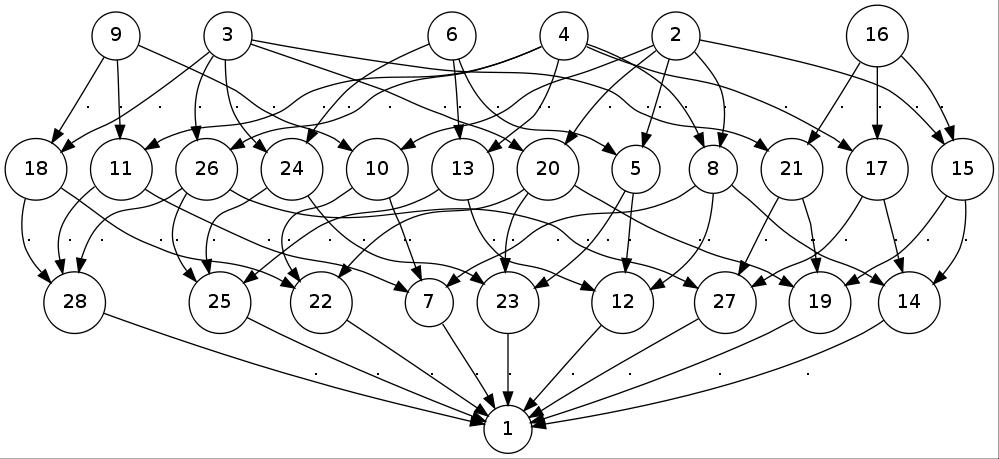
\includegraphics[height=3cm,keepaspectratio=true]{fornaess-sibony.jpg}   }

 

\subsection{\textcolor{Chapter }{PoirierExamples}}
\logpage{[ 10, 1, 5 ]}\nobreak
\hyperdef{L}{X8700DB2886B0A7E4}{}
{\noindent\textcolor{FuncColor}{$\triangleright$\ \ \texttt{PoirierExamples({\mdseries\slshape ...})\index{PoirierExamples@\texttt{PoirierExamples}}
\label{PoirierExamples}
}\hfill{\scriptsize (function)}}\\


 The examples from Poirier's paper \cite{math.DS/9305207}. See details under \texttt{PolynomialIMGMachine} (\ref{PolynomialIMGMachine}); in particular, \texttt{PoirierExamples(1)} is the Douady rabbit map. }

 

\subsection{\textcolor{Chapter }{AddingGroup}}
\logpage{[ 10, 1, 6 ]}\nobreak
\hyperdef{L}{X85F4FDF787173863}{}
{\noindent\textcolor{FuncColor}{$\triangleright$\ \ \texttt{AddingGroup({\mdseries\slshape n})\index{AddingGroup@\texttt{AddingGroup}}
\label{AddingGroup}
}\hfill{\scriptsize (function)}}\\
\noindent\textcolor{FuncColor}{$\triangleright$\ \ \texttt{AddingMachine({\mdseries\slshape n})\index{AddingMachine@\texttt{AddingMachine}}
\label{AddingMachine}
}\hfill{\scriptsize (function)}}\\
\noindent\textcolor{FuncColor}{$\triangleright$\ \ \texttt{AddingElement({\mdseries\slshape n})\index{AddingElement@\texttt{AddingElement}}
\label{AddingElement}
}\hfill{\scriptsize (function)}}\\


 The second function constructs the adding machine on the alphabet \texttt{[1..n]}. This machine has a trivial state 1, and a non-trivial state 2. It implements
the operation "add 1 with carry" on sequences. 

 The third function constructs the Mealy element on the adding machine, with
initial state 2. 

 The first function constructs the state-closed group generated by the adding
machine on \texttt{[1..n]}. This group is isomorphic to the \texttt{Integers}. 
\begin{Verbatim}[commandchars=!@B,fontsize=\small,frame=single,label=Example]
  !gapprompt@gap>B !gapinput@Display(AddingElement(3));B
     |  1     2     3
  ---+-----+-----+-----+
   a | a,1   a,2   a,3
   b | a,2   a,3   b,1
  ---+-----+-----+-----+
  Initial state: b
  !gapprompt@gap>B !gapinput@ActivityPerm(FRElement(AddingMachine(3),2),2);B
  (1,4,7,2,5,8,3,6,9)
  !gapprompt@gap>B !gapinput@G := AddingGroup(3);B
  <self-similar group over [ 1 .. 3 ] with 1 generator>
  !gapprompt@gap>B !gapinput@Size(G);B
  infinity
  !gapprompt@gap>B !gapinput@IsRecurrentFRSemigroup(G);B
  true
  !gapprompt@gap>B !gapinput@IsLevelTransitive(G);B
  true
\end{Verbatim}
 }

 

\subsection{\textcolor{Chapter }{BinaryAddingGroup}}
\logpage{[ 10, 1, 7 ]}\nobreak
\hyperdef{L}{X7A4BB24A805CDF63}{}
{\noindent\textcolor{FuncColor}{$\triangleright$\ \ \texttt{BinaryAddingGroup\index{BinaryAddingGroup@\texttt{BinaryAddingGroup}}
\label{BinaryAddingGroup}
}\hfill{\scriptsize (global variable)}}\\
\noindent\textcolor{FuncColor}{$\triangleright$\ \ \texttt{BinaryAddingMachine\index{BinaryAddingMachine@\texttt{BinaryAddingMachine}}
\label{BinaryAddingMachine}
}\hfill{\scriptsize (global variable)}}\\
\noindent\textcolor{FuncColor}{$\triangleright$\ \ \texttt{BinaryAddingElement\index{BinaryAddingElement@\texttt{BinaryAddingElement}}
\label{BinaryAddingElement}
}\hfill{\scriptsize (global variable)}}\\


 These are respectively the same as \texttt{AddingGroup(2)}, \texttt{AddingMachine(2)} and \texttt{AddingElement(2)}. }

 

\subsection{\textcolor{Chapter }{MixerGroup}}
\logpage{[ 10, 1, 8 ]}\nobreak
\hyperdef{L}{X78AFA63B86C94227}{}
{\noindent\textcolor{FuncColor}{$\triangleright$\ \ \texttt{MixerGroup({\mdseries\slshape A, B, f[, g]})\index{MixerGroup@\texttt{MixerGroup}}
\label{MixerGroup}
}\hfill{\scriptsize (function)}}\\
\noindent\textcolor{FuncColor}{$\triangleright$\ \ \texttt{MixerMachine({\mdseries\slshape A, B, f[, g]})\index{MixerMachine@\texttt{MixerMachine}}
\label{MixerMachine}
}\hfill{\scriptsize (function)}}\\
\textbf{\indent Returns:\ }
A Mealy "mixer" machine/group.



 The second function constructs a Mealy "mixer" machine \texttt{m}. This is a machine determined by a permutation group \mbox{\texttt{\mdseries\slshape A}}, a finitely generated group \mbox{\texttt{\mdseries\slshape B}}, and a matrix of homomorphisms from \mbox{\texttt{\mdseries\slshape B}} to \mbox{\texttt{\mdseries\slshape A}}. If \mbox{\texttt{\mdseries\slshape A}} acts on \texttt{[1..d]}, then each row of \mbox{\texttt{\mdseries\slshape f}} contains at most $d-1$ homomorphisms. The optional last argument is an endomorphism of \mbox{\texttt{\mdseries\slshape B}}. If absent, it is treated as the identity map on \mbox{\texttt{\mdseries\slshape B}}. 

 The states of the machine are 1, followed by some elements \texttt{a} of \mbox{\texttt{\mdseries\slshape A}}, followed by as many copies of some elements \texttt{b} of \mbox{\texttt{\mdseries\slshape B}} as there are rows in \mbox{\texttt{\mdseries\slshape f}}. The elements in \mbox{\texttt{\mdseries\slshape B}} that are taken is the smallest sublist of \mbox{\texttt{\mdseries\slshape B}} containing its generators and closed under \mbox{\texttt{\mdseries\slshape g}}. The elements in \mbox{\texttt{\mdseries\slshape A}} that are taken are the generators of \mbox{\texttt{\mdseries\slshape A}} and all images of all taken elements of \mbox{\texttt{\mdseries\slshape B}} under maps in \mbox{\texttt{\mdseries\slshape f}}. 

 The transitions from \texttt{a} are towards 1 and the outputs are the permutations in \mbox{\texttt{\mdseries\slshape A}}. The transitions from \texttt{b} are periodically given by \mbox{\texttt{\mdseries\slshape f}}, completed by trivial elements, and finally by $b^g$; the output of \texttt{b} is trivial. 

 This construction is described in more detail in \cite{MR1856923} and \cite{MR2035113}. 

 \texttt{Correspondence(m)} is a list, with in first position the subset of the states that correspond to \mbox{\texttt{\mdseries\slshape A}}, in second position the states that correspond to the first copy of \mbox{\texttt{\mdseries\slshape B}}, etc. 

 The first function constructs the group generated by the mixer machine. For
examples see \texttt{GrigorchukGroups} (\ref{GrigorchukGroups}), \texttt{NeumannGroup} (\ref{NeumannGroup}), \texttt{GuptaSidkiGroups} (\ref{GuptaSidkiGroups}), and \texttt{ZugadiSpinalGroup} (\ref{ZugadiSpinalGroup}). 
\begin{Verbatim}[commandchars=!@|,fontsize=\small,frame=single,label=Example]
  !gapprompt@gap>| !gapinput@grigorchukgroup := MixerGroup(Group((1,2)),Group((1,2)),|
       [[IdentityMapping(Group((1,2)))],[IdentityMapping(Group((1,2)))],[]]));
  <self-similar group over [ 1 .. 2 ] with 4 generators>
  !gapprompt@gap>| !gapinput@IdGroup(Group(grigorchukgroup.1,grigorchukgroup.2));|
  [ 32, 18 ]
\end{Verbatim}
 }

 

\subsection{\textcolor{Chapter }{SunicGroup}}
\logpage{[ 10, 1, 9 ]}\nobreak
\hyperdef{L}{X84C97E0687F119C0}{}
{\noindent\textcolor{FuncColor}{$\triangleright$\ \ \texttt{SunicGroup({\mdseries\slshape phi})\index{SunicGroup@\texttt{SunicGroup}}
\label{SunicGroup}
}\hfill{\scriptsize (function)}}\\
\noindent\textcolor{FuncColor}{$\triangleright$\ \ \texttt{SunicMachine({\mdseries\slshape phi})\index{SunicMachine@\texttt{SunicMachine}}
\label{SunicMachine}
}\hfill{\scriptsize (function)}}\\
\textbf{\indent Returns:\ }
The Sunic machine associated with the polynomial \mbox{\texttt{\mdseries\slshape phi}}.



 A "Sunic machine" is a special kind of \texttt{MixerMachine} (\ref{MixerMachine}), in which the group $A$ is a finite field $GF(q)$, the group $B$ is an extension $A[x]/(\phi)$, where $\phi$ is a monic polynomial; there is a map $f:B\to A$, given say by evaluation; and there is an endomorphism of $g:B\to B$ given by multiplication by $\phi$. 

 These groups were described in \cite{MR2318546}. In particular, the case $q=2$ and $\phi=x^2+x+1$ gives the original \texttt{GrigorchukGroup} (\ref{GrigorchukGroup}). 
\begin{Verbatim}[commandchars=!@|,fontsize=\small,frame=single,label=Example]
  !gapprompt@gap>| !gapinput@x := Indeterminate(GF(2));;|
  !gapprompt@gap>| !gapinput@g := SunicGroup(x^2+x+1);|
  SunicGroup(x^2+x+Z(2)^0)
  !gapprompt@gap>| !gapinput@g = GrigorchukGroup;|
  true
\end{Verbatim}
 }

 

\subsection{\textcolor{Chapter }{GrigorchukMachines}}
\logpage{[ 10, 1, 10 ]}\nobreak
\hyperdef{L}{X79E3F3BE80F34590}{}
{\noindent\textcolor{FuncColor}{$\triangleright$\ \ \texttt{GrigorchukMachines({\mdseries\slshape omega})\index{GrigorchukMachines@\texttt{GrigorchukMachines}}
\label{GrigorchukMachines}
}\hfill{\scriptsize (function)}}\\
\noindent\textcolor{FuncColor}{$\triangleright$\ \ \texttt{GrigorchukGroups({\mdseries\slshape omega})\index{GrigorchukGroups@\texttt{GrigorchukGroups}}
\label{GrigorchukGroups}
}\hfill{\scriptsize (function)}}\\
\textbf{\indent Returns:\ }
One of the Grigorchuk groups.



 This function constructs the Grigorchuk machine or group associated with the
infinite sequence \mbox{\texttt{\mdseries\slshape omega}}, which is assumed (pre)periodic; \mbox{\texttt{\mdseries\slshape omega}} is either a periodic list (see \texttt{PeriodicList} (\ref{PeriodicList})) or a plain list describing the period. Entries in the list are integers in \texttt{[1..3]}. 

 These groups are \texttt{MixerGroup} (\ref{MixerGroup})s. The most famous example is \texttt{GrigorchukGroups([1,2,3])}, which is also called \texttt{GrigorchukGroup} (\ref{GrigorchukGroup}). 

 These groups are all 4-generated and infinite. They are described in \cite{MR764305}. \texttt{GrigorchukGroups([1])} is infinite dihedral. If \mbox{\texttt{\mdseries\slshape omega}} contains at least 2 different digits, \texttt{GrigorchukGroups([1])} has intermediate word growth. If \mbox{\texttt{\mdseries\slshape omega}} contains all 3 digits, \texttt{GrigorchukGroups([1])} is torsion. 

 The growth of \texttt{GrigorchukGroups([1,2])} has been studied in \cite{MR2144977}. 
\begin{Verbatim}[commandchars=!@|,fontsize=\small,frame=single,label=Example]
  !gapprompt@gap>| !gapinput@G := GrigorchukGroups([1]);|
  GrigorchukGroups([ 1 ])
  !gapprompt@gap>| !gapinput@Index(G,DerivedSubgroup(G)); IsAbelian(DerivedSubgroup(G));|
  4
  true
  !gapprompt@gap>| !gapinput@H := GrigorchukGroups([1,2]);|
  GrigorchukGroups([ 1, 2 ])
  !gapprompt@gap>| !gapinput@Order(H.1*H.2);|
  8
  !gapprompt@gap>| !gapinput@Order(H.1*H.4);|
  infinity
  !gapprompt@gap>| !gapinput@IsSubgroup(H,G);|
  true
\end{Verbatim}
 }

 

\subsection{\textcolor{Chapter }{GrigorchukMachine}}
\logpage{[ 10, 1, 11 ]}\nobreak
\hyperdef{L}{X85BAE48780E665A4}{}
{\noindent\textcolor{FuncColor}{$\triangleright$\ \ \texttt{GrigorchukMachine\index{GrigorchukMachine@\texttt{GrigorchukMachine}}
\label{GrigorchukMachine}
}\hfill{\scriptsize (global variable)}}\\
\noindent\textcolor{FuncColor}{$\triangleright$\ \ \texttt{GrigorchukGroup\index{GrigorchukGroup@\texttt{GrigorchukGroup}}
\label{GrigorchukGroup}
}\hfill{\scriptsize (global variable)}}\\


 This is Grigorchuk's first group, introduced in \cite{MR565099}. It is a 4-generated infinite torsion group, and has intermediate word
growth. It could have been defined as \texttt{FRGroup("a=(1,2)","b={\textless}a,c{\textgreater}","c={\textless}a,d{\textgreater}","d={\textless},b{\textgreater}")}, but is rather defined using Mealy elements. 

 The command \texttt{EpimorphismFromFpGroup(GrigorchukGroup,n)} constructs an approximating presentation for the Grigorchuk group, as proven
in \cite{MR819415}. Adding the relations \texttt{Image(sigma\texttt{\symbol{94}}(n-2),(a*d)\texttt{\symbol{94}}2)}, \texttt{Image(sigma\texttt{\symbol{94}}(n-1),(a*b)\texttt{\symbol{94}}2)} and \texttt{Image(sigma\texttt{\symbol{94}}(n-2),(a*c)\texttt{\symbol{94}}4)} yields the quotient acting on $2^n$ points, as a finitely presented group. }

 

\subsection{\textcolor{Chapter }{GrigorchukOverGroup}}
\logpage{[ 10, 1, 12 ]}\nobreak
\hyperdef{L}{X800640597E9C707D}{}
{\noindent\textcolor{FuncColor}{$\triangleright$\ \ \texttt{GrigorchukOverGroup\index{GrigorchukOverGroup@\texttt{GrigorchukOverGroup}}
\label{GrigorchukOverGroup}
}\hfill{\scriptsize (global variable)}}\\


 This is a group strictly containing the Grigorchuk group (see \texttt{GrigorchukGroup} (\ref{GrigorchukGroup})). It also has intermediate growth (see \cite{MR1899368}, but it contains elements of infinite order. It could have been defined as \texttt{FRGroup("a=(1,2)","b={\textless}a,c{\textgreater}","c={\textless},d{\textgreater}","d={\textless},b{\textgreater}")}, but is rather defined using Mealy elements. 
\begin{Verbatim}[commandchars=!@|,fontsize=\small,frame=single,label=Example]
  !gapprompt@gap>| !gapinput@IsSubgroup(GrigorchukOverGroup,GrigorchukGroup);|
  true
  !gapprompt@gap>| !gapinput@Order(Product(GeneratorsOfGroup(GrigorchukOverGroup)));|
  infinity
  !gapprompt@gap>| !gapinput@GrigorchukGroup.2=GrigorchukSuperGroup.2*GrigorchukSuperGroup.3;|
  true
\end{Verbatim}
 

 The command \texttt{EpimorphismFromFpGroup(GrigorchukOverGroup,n)} will will construct an approximating presentation for the Grigorchuk
overgroup, as proven in \cite{MR2009317}. }

 

\subsection{\textcolor{Chapter }{GrigorchukTwistedTwin}}
\logpage{[ 10, 1, 13 ]}\nobreak
\hyperdef{L}{X7E765AF77AAC21A6}{}
{\noindent\textcolor{FuncColor}{$\triangleright$\ \ \texttt{GrigorchukTwistedTwin\index{GrigorchukTwistedTwin@\texttt{GrigorchukTwistedTwin}}
\label{GrigorchukTwistedTwin}
}\hfill{\scriptsize (global variable)}}\\


 This is a group with same closure as the Grigorchuk group (see \texttt{GrigorchukGroup} (\ref{GrigorchukGroup})), but not isomorphic to it. It could have been defined as \texttt{FRGroup("a=(1,2)","x={\textless}y,a{\textgreater}","y={\textless}a,z{\textgreater}","z={\textless},x{\textgreater}")}, but is rather defined using Mealy elements. 
\begin{Verbatim}[commandchars=!@|,fontsize=\small,frame=single,label=Example]
  !gapprompt@gap>| !gapinput@AbelianInvariants(GrigorchukTwistedTwin);|
  [ 2, 2, 2, 2 ]
  !gapprompt@gap>| !gapinput@AbelianInvariants(GrigorchukGroup);|
  [ 2, 2, 2 ]
  !gapprompt@gap>| !gapinput@PermGroup(GrigorchukGroup,8)=PermGroup(GrigorchukTwistedTwin,8);|
  true
\end{Verbatim}
 }

 

\subsection{\textcolor{Chapter }{BrunnerSidkiVieiraGroup}}
\logpage{[ 10, 1, 14 ]}\nobreak
\hyperdef{L}{X7F93EC437B5AE276}{}
{\noindent\textcolor{FuncColor}{$\triangleright$\ \ \texttt{BrunnerSidkiVieiraGroup\index{BrunnerSidkiVieiraGroup@\texttt{BrunnerSidkiVieiraGroup}}
\label{BrunnerSidkiVieiraGroup}
}\hfill{\scriptsize (global variable)}}\\
\noindent\textcolor{FuncColor}{$\triangleright$\ \ \texttt{BrunnerSidkiVieiraMachine\index{BrunnerSidkiVieiraMachine@\texttt{BrunnerSidkiVieiraMachine}}
\label{BrunnerSidkiVieiraMachine}
}\hfill{\scriptsize (global variable)}}\\


 This machine is the sum of two adding machines, one in standard form and one
conjugated by the element \texttt{d} described below. The group that it generates is described in \cite{MR1656573}. It could have been defined as \texttt{FRGroup("tau={\textless},tau{\textgreater}(1,2)","mu={\textless},mu\texttt{\symbol{94}}-1{\textgreater}(1,2)")}, but is rather defined using Mealy elements. 
\begin{Verbatim}[commandchars=!@C,fontsize=\small,frame=single,label=Example]
  !gapprompt@gap>C !gapinput@V := FRGroup("d=<e,e>(1,2)","e=<d,d>");C
  <self-similar group over [ 1 .. 2 ] with 2 generators>
  !gapprompt@gap>C !gapinput@Elements(V);C
  [ <2|identity ...>, <2|e>, <2|d>, <2|e*d> ]
  !gapprompt@gap>C !gapinput@AssignGeneratorVariables(BrunnerSidkiVieiraGroup);C
  #I  Assigned the global variables [ "tau", "mu", "" ]
  !gapprompt@gap>C !gapinput@List(V,x->tau^x)=[tau,mu,mu^-1,tau^-1];C
  true
\end{Verbatim}
 }

 

\subsection{\textcolor{Chapter }{AleshinGroups}}
\logpage{[ 10, 1, 15 ]}\nobreak
\hyperdef{L}{X7F8A028B799946D3}{}
{\noindent\textcolor{FuncColor}{$\triangleright$\ \ \texttt{AleshinGroups({\mdseries\slshape l})\index{AleshinGroups@\texttt{AleshinGroups}}
\label{AleshinGroups}
}\hfill{\scriptsize (function)}}\\
\noindent\textcolor{FuncColor}{$\triangleright$\ \ \texttt{AleshinMachines({\mdseries\slshape l})\index{AleshinMachines@\texttt{AleshinMachines}}
\label{AleshinMachines}
}\hfill{\scriptsize (function)}}\\
\textbf{\indent Returns:\ }
The Aleshin machine with \texttt{Length(l)} states.



 This function constructs the bireversible machines introduced by Aleshin in \cite{MR713968}. The argument \mbox{\texttt{\mdseries\slshape l}} is a list of permutations, either \texttt{()} or \texttt{(1,2)}. The groups that they generate are contructed as \texttt{AleshinGroups}. 

 If \texttt{l=[(1,2),(1,2),()]}, this is \texttt{AleshinGroup} (\ref{AleshinGroup}). More generally, if \texttt{l=[(1,2,(1,2),(),...,()]} has odd length, this is a free group of rank \texttt{Length(l)}, see \cite{MR2318547} and \cite{0604328}. 

 If \texttt{l=[(1,2),(1,2),...]} has even length and contains an even number of \texttt{()}'s, then this is also a free group of rank \texttt{Length(l)}, see \cite{0610033}. 

 If \texttt{l=[(),(),(1,2)]}, this is \texttt{BabyAleshinGroup} (\ref{BabyAleshinGroup}). more generally, if \texttt{l=[(),(),...]} has even length and contains an even number of \texttt{(1,2)}'s, then this is the free product of \texttt{Length(l)} copies of the order-2 group. }

 

\subsection{\textcolor{Chapter }{AleshinGroup}}
\logpage{[ 10, 1, 16 ]}\nobreak
\hyperdef{L}{X7C286D3A84790ECE}{}
{\noindent\textcolor{FuncColor}{$\triangleright$\ \ \texttt{AleshinGroup\index{AleshinGroup@\texttt{AleshinGroup}}
\label{AleshinGroup}
}\hfill{\scriptsize (global variable)}}\\
\noindent\textcolor{FuncColor}{$\triangleright$\ \ \texttt{AleshinMachine\index{AleshinMachine@\texttt{AleshinMachine}}
\label{AleshinMachine}
}\hfill{\scriptsize (global variable)}}\\


 This is the first example of non-abelian free group. It is the group generated
by \texttt{AleshinMachine([(1,2),(1,2),()])}. It could have been defined as \texttt{FRGroup("a={\textless}b,c{\textgreater}(1,2)","b={\textless}c,b{\textgreater}(1,2)","c={\textless}a,a{\textgreater}")}, but is rather defined using Mealy elements. }

 

\subsection{\textcolor{Chapter }{BabyAleshinGroup}}
\logpage{[ 10, 1, 17 ]}\nobreak
\hyperdef{L}{X7E024B4D7BA411B1}{}
{\noindent\textcolor{FuncColor}{$\triangleright$\ \ \texttt{BabyAleshinGroup\index{BabyAleshinGroup@\texttt{BabyAleshinGroup}}
\label{BabyAleshinGroup}
}\hfill{\scriptsize (global variable)}}\\
\noindent\textcolor{FuncColor}{$\triangleright$\ \ \texttt{BabyAleshinMachine\index{BabyAleshinMachine@\texttt{BabyAleshinMachine}}
\label{BabyAleshinMachine}
}\hfill{\scriptsize (global variable)}}\\


 There are only two connected, transitive bireversible machines on a 2-letter
alphabet, with 3 generators: \texttt{AleshinMachine(3)} and the baby Aleshin machine. 

 The group generated by this machine is abstractly the free product of three $C_2$'s, see \cite[1.10.3]{MR2162164}. It could have been defined as \texttt{FRGroup("a={\textless}b,c{\textgreater}","b={\textless}c,b{\textgreater}","c={\textless}a,a{\textgreater}(1,2)")}, but is rather defined here using Mealy elements. 
\begin{Verbatim}[commandchars=!@|,fontsize=\small,frame=single,label=Example]
  !gapprompt@gap>| !gapinput@K := Kernel(GroupHomomorphismByImagesNC(BabyAleshinGroup,Group((1,2)),|
                   GeneratorsOfGroup(BabyAleshinGroup),[(1,2),(1,2),(1,2)]));
  <self-similar group over [ 1 .. 2 ] with 4 generators>
  !gapprompt@gap>| !gapinput@Index(BabyAleshinGroup,K);|
  2
  !gapprompt@gap>| !gapinput@IsSubgroup(AleshinGroup,K);|
  true
\end{Verbatim}
 }

 

\subsection{\textcolor{Chapter }{SidkiFreeGroup}}
\logpage{[ 10, 1, 18 ]}\nobreak
\hyperdef{L}{X8108E3A8872A6FFE}{}
{\noindent\textcolor{FuncColor}{$\triangleright$\ \ \texttt{SidkiFreeGroup\index{SidkiFreeGroup@\texttt{SidkiFreeGroup}}
\label{SidkiFreeGroup}
}\hfill{\scriptsize (global variable)}}\\


 This is a group suggested by Sidki as an example of a non-abelian state-closed
free group. Nothing is known about that group: whether it is free as
conjectured; whether generator \mbox{\texttt{\mdseries\slshape a}} is state-closed, etc. It is defined as \texttt{FRGroup("a={\textless}a\texttt{\symbol{94}}2,a\texttt{\symbol{94}}t{\textgreater}","t={\textless},t{\textgreater}(1,2)")]]{\textgreater}}. }

 

\subsection{\textcolor{Chapter }{GuptaSidkiGroups}}
\logpage{[ 10, 1, 19 ]}\nobreak
\hyperdef{L}{X82D3CB6A7C189C78}{}
{\noindent\textcolor{FuncColor}{$\triangleright$\ \ \texttt{GuptaSidkiGroups({\mdseries\slshape n})\index{GuptaSidkiGroups@\texttt{GuptaSidkiGroups}}
\label{GuptaSidkiGroups}
}\hfill{\scriptsize (function)}}\\
\noindent\textcolor{FuncColor}{$\triangleright$\ \ \texttt{GeneralizedGuptaSidkiGroups({\mdseries\slshape n})\index{GeneralizedGuptaSidkiGroups@\texttt{GeneralizedGuptaSidkiGroups}}
\label{GeneralizedGuptaSidkiGroups}
}\hfill{\scriptsize (function)}}\\
\noindent\textcolor{FuncColor}{$\triangleright$\ \ \texttt{GuptaSidkiMachines({\mdseries\slshape n})\index{GuptaSidkiMachines@\texttt{GuptaSidkiMachines}}
\label{GuptaSidkiMachines}
}\hfill{\scriptsize (function)}}\\
\textbf{\indent Returns:\ }
The Gupta-Sidki group/machine on an \mbox{\texttt{\mdseries\slshape n}}-letter alphabet.



 This function constructs the machines introduced by Gupta and Sidki in \cite{MR696534}. They generate finitely generated infinite torsion groups: the exponent of
every element divides some power of \mbox{\texttt{\mdseries\slshape n}}. The special case $n=3$ is defined as \texttt{GuptaSidkiGroup} (\ref{GuptaSidkiGroup}) and \texttt{GuptaSidkiMachine} (\ref{GuptaSidkiMachine}). 

 For $n>3$, there are (at least) two natural ways to generalize the Gupta-Sidki
construction: the original one involves the recursion \texttt{"t={\textless}a,a\texttt{\symbol{94}}-1,1,...,1,t{\textgreater}"}, while the second (called here `generalized') involves the recursion \texttt{"t={\textless}a,a\texttt{\symbol{94}}2,...,a\texttt{\symbol{94}}-1,t{\textgreater}"}. A finite L-presentation for the latter is implemented. It is not as
computationally efficient as the L-presentation of the normal closure of \texttt{t} (a subgroup of index $p$), which is an ascending L-presented group. The inclusion of that subgroup may
be recoverd via \texttt{EmbeddingOfAscendingSubgroup(GuptaSidkiGroup)}. }

 

\subsection{\textcolor{Chapter }{GuptaSidkiGroup}}
\logpage{[ 10, 1, 20 ]}\nobreak
\hyperdef{L}{X83E59288860EF661}{}
{\noindent\textcolor{FuncColor}{$\triangleright$\ \ \texttt{GuptaSidkiGroup\index{GuptaSidkiGroup@\texttt{GuptaSidkiGroup}}
\label{GuptaSidkiGroup}
}\hfill{\scriptsize (global variable)}}\\
\noindent\textcolor{FuncColor}{$\triangleright$\ \ \texttt{GuptaSidkiMachine\index{GuptaSidkiMachine@\texttt{GuptaSidkiMachine}}
\label{GuptaSidkiMachine}
}\hfill{\scriptsize (global variable)}}\\


 This is an infinite, 2-generated, torsion 3-group. It could have been defined
as \texttt{FRGroup("a=(1,2,3)","t={\textless}a,a\texttt{\symbol{94}}-1,t{\textgreater}")}, but is rather defined using Mealy elements. }

 

\subsection{\textcolor{Chapter }{NeumannGroup}}
\logpage{[ 10, 1, 21 ]}\nobreak
\hyperdef{L}{X8521B4FF7BA189B2}{}
{\noindent\textcolor{FuncColor}{$\triangleright$\ \ \texttt{NeumannGroup({\mdseries\slshape P})\index{NeumannGroup@\texttt{NeumannGroup}}
\label{NeumannGroup}
}\hfill{\scriptsize (function)}}\\
\noindent\textcolor{FuncColor}{$\triangleright$\ \ \texttt{NeumannMachine({\mdseries\slshape P})\index{NeumannMachine@\texttt{NeumannMachine}}
\label{NeumannMachine}
}\hfill{\scriptsize (function)}}\\
\textbf{\indent Returns:\ }
The Neumann group/machine on the permutation group \mbox{\texttt{\mdseries\slshape P}}.



 The first function constructs the Neumann group associated with the
permutation group \mbox{\texttt{\mdseries\slshape P}}. These groups were first considered in \cite{MR840129}. In particular, \texttt{NeumannGroup(PSL(3,2))} is a group of non-uniform exponential growth (see \cite{MR1981466}), and \texttt{NeumannGroup(Group((1,2,3)))} is \texttt{FabrykowskiGuptaGroup} (\ref{FabrykowskiGuptaGroup}). 

 The second function constructs the Neumann machine associated to the
permutation group \mbox{\texttt{\mdseries\slshape P}}. It is a shortcut for \texttt{MixerMachine(P,P,[[IdentityMapping(P)]])}. 

 The attribute \texttt{Correspondence(G)} is set to a list of homomorphisms from \mbox{\texttt{\mdseries\slshape P}} to the \texttt{A} and \texttt{B} copies of \texttt{P}. }

 

\subsection{\textcolor{Chapter }{FabrykowskiGuptaGroup}}
\logpage{[ 10, 1, 22 ]}\nobreak
\hyperdef{L}{X878D1C7080EA9797}{}
{\noindent\textcolor{FuncColor}{$\triangleright$\ \ \texttt{FabrykowskiGuptaGroup\index{FabrykowskiGuptaGroup@\texttt{FabrykowskiGuptaGroup}}
\label{FabrykowskiGuptaGroup}
}\hfill{\scriptsize (global variable)}}\\
\noindent\textcolor{FuncColor}{$\triangleright$\ \ \texttt{FabrykowskiGuptaGroups({\mdseries\slshape p})\index{FabrykowskiGuptaGroups@\texttt{FabrykowskiGuptaGroups}}
\label{FabrykowskiGuptaGroups}
}\hfill{\scriptsize (function)}}\\


 This is an infinite, 2-generated group of intermediate word growth. It was
studied in \cite{MR942349} and \cite{MR1153150}. It could have been defined as \texttt{FRGroup("a=(1,2,3)","t={\textless}a,,t{\textgreater}")}, but is rather defined using Mealy elements. It has a torsion-free subgroup
of index 3 and is branched. 

 The natural generalization, replacing 3 by $p$, is constructed by the second form. It is a specific case of Neumann group
(see \texttt{NeumannGroup} (\ref{NeumannGroup})), for which an ascending L-presentation is known. }

 

\subsection{\textcolor{Chapter }{ZugadiSpinalGroup}}
\logpage{[ 10, 1, 23 ]}\nobreak
\hyperdef{L}{X7C5ADAE77EA3876D}{}
{\noindent\textcolor{FuncColor}{$\triangleright$\ \ \texttt{ZugadiSpinalGroup\index{ZugadiSpinalGroup@\texttt{ZugadiSpinalGroup}}
\label{ZugadiSpinalGroup}
}\hfill{\scriptsize (global variable)}}\\


 This is an infinite, 2-generated group, which was studied in \cite{MR1899368}. It has a torsion-free subgroup of index 3, and is virtually branched but not
branched. It could have been defined as \texttt{FRGroup("a=(1,2,3)","t={\textless}a,a,t{\textgreater}")}, but is rather defined using Mealy elements. 

 Amaia Zugadi computed its Hausdorff dimension to be $1/2$. }

 

\subsection{\textcolor{Chapter }{GammaPQMachine}}
\logpage{[ 10, 1, 24 ]}\nobreak
\hyperdef{L}{X7A0319827CB51ED0}{}
{\noindent\textcolor{FuncColor}{$\triangleright$\ \ \texttt{GammaPQMachine({\mdseries\slshape p, q})\index{GammaPQMachine@\texttt{GammaPQMachine}}
\label{GammaPQMachine}
}\hfill{\scriptsize (function)}}\\
\noindent\textcolor{FuncColor}{$\triangleright$\ \ \texttt{GammaPQGroup({\mdseries\slshape p, q})\index{GammaPQGroup@\texttt{GammaPQGroup}}
\label{GammaPQGroup}
}\hfill{\scriptsize (function)}}\\
\textbf{\indent Returns:\ }
The quaternion-based machine / SC group.



 The first function constructs a bireversible (see \texttt{IsBireversible} (\ref{IsBireversible})) Mealy machine based on quaternions, see \cite{MR1839488} and \cite{MR1839489}. This machine has $p+1$ states indexed by integer quaternions of norm \mbox{\texttt{\mdseries\slshape p}}, and an alphabet of size $q+1$ indexed by quaternions of norm \mbox{\texttt{\mdseries\slshape q}}. These quaternions are congruent to $1\pmod 2$ or $i\pmod 2$ depending on whether the odd prime $p$ or $q$ is $1$ or $3\pmod 4$. 

 The structure of the machine is such that there is a transition from $(q,a)$ to $(q',a')$ precisely when $qa'=\pm q'a$. In particular, the relations of the \texttt{StructuralGroup} (\ref{StructuralGroup}) hold up to a sign, when the alphabet/state letters are substituted for the
appropriate quaternions. 

 The quaternions themselves can be recovered through \texttt{Correspondence} (\ref{Correspondence:FR machine}), which is a list with in first position the quaternions of norm $p$ and in second those of norm $q$. 

 The second function constructs the quaternion lattice that is the \texttt{StructuralGroup} (\ref{StructuralGroup}) of that machine. It has actions on two trees, given by \texttt{VerticalAction} (\ref{VerticalAction}) and \texttt{HorizontalAction} (\ref{HorizontalAction}); the ranges of these actions are groups generated by automata, which are
infinitely-transitive (see \texttt{IsInfinitelyTransitive} (\ref{IsInfinitelyTransitive})) and free by \cite[Proposition 3.3]{MR2155175}; see also \cite{MR713968}. }

 

\subsection{\textcolor{Chapter }{RattaggiGroup}}
\logpage{[ 10, 1, 25 ]}\nobreak
\hyperdef{L}{X80B617717C2887D4}{}
{\noindent\textcolor{FuncColor}{$\triangleright$\ \ \texttt{RattaggiGroup\index{RattaggiGroup@\texttt{RattaggiGroup}}
\label{RattaggiGroup}
}\hfill{\scriptsize (global variable)}}\\


 This record contains interesting examples of VH groups, that were studied by
Rattaggi in his PhD thesis \cite{Rattaggi}. His Example 2.x appears as \texttt{RattaggiGroup.2{\textunderscore}x}. 

 The following summary of the examples' properties are copied from Rattaggi's
thesis. RF means "residually finite"; JI means "just infinite"; VS means
"virtually simple". \begin{center}
\begin{tabular}{r|c|c|c|c|c|c|c}Example&
$P_h$&
$P_v$&
Irred?&
Linear?&
RF?&
JI?&
VS?\\
\hline
2.2&
2tr&
2tr&
Y&
N&
N?&
Y&
Y?\\
2.15\\
2.18\\
2.21\\
2.26&
2tr&
q-prim&
Y&
N&
N&
N&
N\\
2.30&
2tr&
2tr&
Y&
N&
N&
Y&
Y?\\
2.36\\
2.39\\
2.43&
2tr&
2tr&
Y&
N&
N&
Y&
Y\\
2.46\\
2.48\\
2.50\\
2.52&
tr&
2tr&
Y&
N&
N&
N&
N\\
2.56\\
2.58&
2tr&
prim&
Y&
N&
N?&
N&
N\\
2.70\\
\hline
3.26&
2tr&
2tr&
Y&
Y&
Y&
Y&
N\\
3.28\\
3.31\\
3.33\\
3.36\\
3.38\\
3.40\\
3.44\\
3.46\\
3.72\\
\end{tabular}\\[2mm]
\end{center}

 }

 

\subsection{\textcolor{Chapter }{HanoiGroup}}
\logpage{[ 10, 1, 26 ]}\nobreak
\hyperdef{L}{X7A0BE9F57B401C5C}{}
{\noindent\textcolor{FuncColor}{$\triangleright$\ \ \texttt{HanoiGroup({\mdseries\slshape n})\index{HanoiGroup@\texttt{HanoiGroup}}
\label{HanoiGroup}
}\hfill{\scriptsize (function)}}\\
\textbf{\indent Returns:\ }
The Hanoi group on an \mbox{\texttt{\mdseries\slshape n}} pegs.



 This function constructs the Hanoi group on \mbox{\texttt{\mdseries\slshape n}} pegs. Generators of the group correspond to moving a peg, and tree vertices
correspond to peg configurations. This group is studied in \cite{MR2217913}. }

 

\subsection{\textcolor{Chapter }{DahmaniGroup}}
\logpage{[ 10, 1, 27 ]}\nobreak
\hyperdef{L}{X7C7A0EEF7EFF8B99}{}
{\noindent\textcolor{FuncColor}{$\triangleright$\ \ \texttt{DahmaniGroup\index{DahmaniGroup@\texttt{DahmaniGroup}}
\label{DahmaniGroup}
}\hfill{\scriptsize (global variable)}}\\


 This is an example of a non-contracting weakly branched group. It was first
studied in \cite{MR2140091}. It could have been defined as \texttt{FRGroup("a={\textless}c,a{\textgreater}(1,2)","b={\textless}b,a{\textgreater}(1,2)","c={\textless}b,c{\textgreater}")}, but is rather defined using Mealy elements. 

 It has relators $abc$, $[a^2c,[a,c]]$, $[cab,a^{-1}c^{-1}ab]$ and $[ac^2,c^{-1}b^{-1}c^2]$ among others. 

 It admits an endomorphism on its derived subgroup. Indeed \texttt{FRElement(1,Comm(a,b))=Comm(c\texttt{\symbol{94}}-1,b/a)}, \texttt{FRElement(1,Comm(a,c))=Comm(a/b,c)}, \texttt{FRElement(1,Comm(b,c))=Comm(c,(a/b)\texttt{\symbol{94}}c)}. }

 

\subsection{\textcolor{Chapter }{MamaghaniGroup}}
\logpage{[ 10, 1, 28 ]}\nobreak
\hyperdef{L}{X7C958AB78484E256}{}
{\noindent\textcolor{FuncColor}{$\triangleright$\ \ \texttt{MamaghaniGroup\index{MamaghaniGroup@\texttt{MamaghaniGroup}}
\label{MamaghaniGroup}
}\hfill{\scriptsize (global variable)}}\\


 This group was studied in \cite{MR2139928}. It is fractal, but not contracting. It could have been defined as \texttt{FRGroup("a={\textless},b{\textgreater}(1,2)","b={\textless}a,c{\textgreater}","c={\textless}a,a\texttt{\symbol{94}}-1{\textgreater}(1,2)")]]{\textgreater}}, but is rather defined using Mealy elements. It partially admits branching on
its subgroup \texttt{Subgroup(G,[a\texttt{\symbol{94}}2,(a\texttt{\symbol{94}}2)\texttt{\symbol{94}}b,(a\texttt{\symbol{94}}2)\texttt{\symbol{94}}c])}, and, setting \texttt{x=Comm(a\texttt{\symbol{94}}2,b)}, on \texttt{Subgroup(G,[x,x\texttt{\symbol{94}}a,x\texttt{\symbol{94}}b,x\texttt{\symbol{94}}(b*a),x\texttt{\symbol{94}}(b/a)])}. One has \texttt{FRElement(1,x)=(x\texttt{\symbol{94}}-1)\texttt{\symbol{94}}b/x}. }

 

\subsection{\textcolor{Chapter }{WeierstrassGroup}}
\logpage{[ 10, 1, 29 ]}\nobreak
\hyperdef{L}{X86D952E8784E4D97}{}
{\noindent\textcolor{FuncColor}{$\triangleright$\ \ \texttt{WeierstrassGroup\index{WeierstrassGroup@\texttt{WeierstrassGroup}}
\label{WeierstrassGroup}
}\hfill{\scriptsize (global variable)}}\\


 This is the iterated monodromy group associated with the Weierstrass $\wp$-function. 

 Some relators in the group: $(atbt)^4$, $((atbt)(bt)^4n)^4$, $((atbt)^2(bt)^4n)^2$. 

 Set $x=[a,t]$, $y=[b,t]$, $z=[c,t]$, and $w=[x,y]$. Then $G'=\langle x,y,z\rangle$ of index 8, and $\gamma_3=\langle[\{x,y,z\},\{a,b,c\}]\rangle$ of index 32, and $\gamma_4=G''=\langle w\rangle^G$, of index 256, and $G''>(G'')^4$ since $[[t^a,t],[t^b,t]]=(w,1,1,1)$. 

 The Schreier graph is obtained in the complex plane as the image of a $2^n\times 2^n$ lattice in the torus, via Weierstrass's $\wp$-function. 

 The element $at$ has infinite order. 

 $[c,t,b][b,t,c][a,t,c][c,t,a]$ has order 2, and belongs to $G''$; so there exist elements of arbitrary large finite order in the group.  }

 

\subsection{\textcolor{Chapter }{FRAffineGroup}}
\logpage{[ 10, 1, 30 ]}\nobreak
\hyperdef{L}{X86B124758135DFBD}{}
{\noindent\textcolor{FuncColor}{$\triangleright$\ \ \texttt{FRAffineGroup({\mdseries\slshape d, R, u[, transversal]})\index{FRAffineGroup@\texttt{FRAffineGroup}}
\label{FRAffineGroup}
}\hfill{\scriptsize (operation)}}\\
\textbf{\indent Returns:\ }
The \mbox{\texttt{\mdseries\slshape d}}-dimensional affine group over \mbox{\texttt{\mdseries\slshape R}}.



 This function constructs a new FR group \texttt{G}, which is finite-index subgroup of the \mbox{\texttt{\mdseries\slshape d}}-dimensional affine group over $R_u$, the local ring over \mbox{\texttt{\mdseries\slshape R}} in which all non-multiples of \mbox{\texttt{\mdseries\slshape u}} are invertible. Since no generators of \texttt{G} are known, \texttt{G} is in fact returned as a full SC group; only its attribute \texttt{Correspondence(G)}, which is a homomorphism from $GL_{d+1}(R_u)$ to \texttt{G}, is relevant. 

 The affine group can also be described as a subgroup of $GL_{d+1}(R_u)$, consisting of those matrices $M$ with $M_{i,d+1}=0$ and $M_{d+1,d+1}=1$. The finite-index subgroup is defined by the conditions $u|M_{i,j}$ for all $j<i$. 

 The only valid arguments are \texttt{R=Integers} and \texttt{R=PolynomialRing(S)} for a finite ring \texttt{S}. The alphabet of the affine group is $R/RuR$; an explicit transversal of $RuR$ be specified as last argument. 

 The following examples construct the "Baumslag-Solitar group" $\mathbb Z[\frac12]\rtimes_2\mathbb Z$ first introduced in \cite{MR0142635}, the "lamplighter group" $(\mathbb Z/2)\wr\mathbb Z$, and a 2-dimensional affine group. Note that the lamplighter group may also
be defined via \texttt{CayleyGroup} (\ref{CayleyGroup}). 
\begin{Verbatim}[commandchars=!@E,fontsize=\small,frame=single,label=Example]
  !gapprompt@gap>E !gapinput@A := FRAffineGroup(1,Integers,3);E
  <self-similar group over [ 1 .. 3 ]>
  !gapprompt@gap>E !gapinput@f := Correspondence(A);E
  MappingByFunction( ( Integers^
  [ 2, 2 ] ), <self-similar group over [ 1 .. 3 ]>, function( mat ) ... end )
  !gapprompt@gap>E !gapinput@BaumslagSolitar := Group([[2,0],[0,1]]^f,[[1,0],[1,1]]^f);E
  <self-similar group over [ 1 .. 3 ] with 2 generators>
  !gapprompt@gap>E !gapinput@BaumslagSolitar.2^BaumslagSolitar.1=BaumslagSolitar.2^2;E
  true
  !gapprompt@gap>E !gapinput@R := PolynomialRing(GF(2));;E
  !gapprompt@gap>E !gapinput@A := FRAffineGroup(1,R,R.1);;E
  !gapprompt@gap>E !gapinput@f := Correspondence(A);;E
  !gapprompt@gap>E !gapinput@Lamplighter := Group(([[1+R.1,0],[0,1]]*One(R))^f,([[1,0],[1,1]]*One(R))^f);E
  <self-similar group over [ 1 .. 2 ] with 2 generators>
  !gapprompt@gap>E !gapinput@Lamplighter = CayleyGroup(Group((1,2)));E
  true
  !gapprompt@gap>E !gapinput@StructureDescription(Group(Lamplighter.2,Lamplighter.2^Lamplighter.1));E
  "C2 x C2"
  !gapprompt@gap>E !gapinput@ForAll([1..10],i->IsOne(Comm(Lamplighter.2,Lamplighter.2^(Lamplighter.1^i))));E
  true
  !gapprompt@gap>E !gapinput@A := FRAffineGroup(2,Integers,2);;E
  !gapprompt@gap>E !gapinput@f := Correspondence(A);;E
  !gapprompt@gap>E !gapinput@a := [[1,4,0],[2,3,0],[1,0,1]];E
  [ [ 1, 4, 0 ], [ 2, 3, 0 ], [ 1, 0, 1 ] ]
  !gapprompt@gap>E !gapinput@b := [[1,2,0],[4,3,0],[0,1,1]];E
  [ [ 1, 2, 0 ], [ 4, 3, 0 ], [ 0, 1, 1 ] ]
  !gapprompt@gap>E !gapinput@Display(b^f);E
      |   1      2
  ----+------+------+
    a |  b,1    c,2
    b |  d,2    e,1
    c |  a,2    f,1
  ...
   bh | cb,1   be,2
   ca | bd,1   bf,2
   cb | ae,2   bh,1
  ----+------+------+
  Initial state:  a
  !gapprompt@gap>E !gapinput@a^f*b^f=(a*b)^f;E
  true
\end{Verbatim}
 }

 

\subsection{\textcolor{Chapter }{CayleyGroup}}
\logpage{[ 10, 1, 31 ]}\nobreak
\hyperdef{L}{X7CFBE31A78F2681B}{}
{\noindent\textcolor{FuncColor}{$\triangleright$\ \ \texttt{CayleyGroup({\mdseries\slshape G})\index{CayleyGroup@\texttt{CayleyGroup}}
\label{CayleyGroup}
}\hfill{\scriptsize (function)}}\\
\noindent\textcolor{FuncColor}{$\triangleright$\ \ \texttt{CayleyMachine({\mdseries\slshape G})\index{CayleyMachine@\texttt{CayleyMachine}}
\label{CayleyMachine}
}\hfill{\scriptsize (function)}}\\
\noindent\textcolor{FuncColor}{$\triangleright$\ \ \texttt{LamplighterGroup({\mdseries\slshape IsFRGroup, G})\index{LamplighterGroup@\texttt{LamplighterGroup}}
\label{LamplighterGroup}
}\hfill{\scriptsize (method)}}\\
\textbf{\indent Returns:\ }
The Cayley machine/group of the group \mbox{\texttt{\mdseries\slshape G}}.



 The \emph{Cayley machine} of a group \mbox{\texttt{\mdseries\slshape G}} is a machine with alphabet and stateset equal to \mbox{\texttt{\mdseries\slshape G}}, and with output and transition functions given by multiplication in the
group, in the order \texttt{state*letter}. 

 The second function constructs a new FR group \texttt{CG}, which acts on \texttt{[1..Size(G)]}. Its generators are in bijection with the elements of \mbox{\texttt{\mdseries\slshape G}}, and have as output the corresponding permutation of \mbox{\texttt{\mdseries\slshape G}} induced by right multiplication, and as transitions all elements of \mbox{\texttt{\mdseries\slshape G}}; see \texttt{CayleyMachine}. This construction was introduced in \cite{MR2197829}. 

 If \mbox{\texttt{\mdseries\slshape G}} is an abelian group, then \texttt{CG} is the wreath product $G\wr\mathbb Z$; it is created by the constructor \texttt{LamplighterGroup(IsFRGroup,G)}. 

 The attribute \texttt{Correspondence(CG)} is a list. Its first entry is a homomorphism from \mbox{\texttt{\mdseries\slshape G}} into \texttt{CG}. Its second entry is the generator of \texttt{CG} that has trivial output. \texttt{CG} is generated \texttt{Correspondence(CG)[2]} and the image of \texttt{Correspondence(CG)[1]}. 

 In the example below, recall the definition of \texttt{Lamplighter} in the example of \texttt{FRAffineGroup} (\ref{FRAffineGroup}). 
\begin{Verbatim}[commandchars=!@A,fontsize=\small,frame=single,label=Example]
  !gapprompt@gap>A !gapinput@L := CayleyGroup(Group((1,2)));A
  CayleyGroup(Group( [ (1,2) ] ))
  !gapprompt@gap>A !gapinput@L=LamplighterGroup(IsFRGroup,CyclicGroup(2));A
  true
  !gapprompt@gap>A !gapinput@(1,2)^Correspondence(L)[1];A
  <Mealy element on alphabet [ 1, 2 ] with 2 states, initial state 1>
  !gapprompt@gap>A !gapinput@IsFinitaryFRElement(last); Display(last2);A
  true
     |  1     2
  ---+-----+-----+
   a | b,2   b,1
   b | b,1   b,2
  ---+-----+-----+
  Initial state: a
\end{Verbatim}
 }

 }

 
\section{\textcolor{Chapter }{Examples of semigroups}}\logpage{[ 10, 2, 0 ]}
\hyperdef{L}{X81B82FA1811AAF8D}{}
{
 

\subsection{\textcolor{Chapter }{I2Machine}}
\logpage{[ 10, 2, 1 ]}\nobreak
\hyperdef{L}{X87541DA582705033}{}
{\noindent\textcolor{FuncColor}{$\triangleright$\ \ \texttt{I2Machine\index{I2Machine@\texttt{I2Machine}}
\label{I2Machine}
}\hfill{\scriptsize (global variable)}}\\
\noindent\textcolor{FuncColor}{$\triangleright$\ \ \texttt{I2Monoid\index{I2Monoid@\texttt{I2Monoid}}
\label{I2Monoid}
}\hfill{\scriptsize (global variable)}}\\


 The Mealy machine $I_2$, and the monoid that it generates. This is the smallest Mealy machine
generating a monoid of intermediate word growth; see \cite{MR2194959}. 

 For sample calculations in this monoid see \texttt{SCSemigroup} (\ref{SCSemigroup}). }

 

\subsection{\textcolor{Chapter }{I4Machine}}
\logpage{[ 10, 2, 2 ]}\nobreak
\hyperdef{L}{X7B32ED3D8715FA4B}{}
{\noindent\textcolor{FuncColor}{$\triangleright$\ \ \texttt{I4Machine\index{I4Machine@\texttt{I4Machine}}
\label{I4Machine}
}\hfill{\scriptsize (global variable)}}\\
\noindent\textcolor{FuncColor}{$\triangleright$\ \ \texttt{I4Monoid\index{I4Monoid@\texttt{I4Monoid}}
\label{I4Monoid}
}\hfill{\scriptsize (global variable)}}\\


 The Mealy machine generating $I_4$, and the monoid that it generates. This is a very small Mealy machine
generating a monoid of intermediate word growth; see \cite{MR2394721}. 

 For sample calculations in this monoid see \texttt{SCMonoid} (\ref{SCMonoid}). }

 }

 
\section{\textcolor{Chapter }{Examples of algebras}}\logpage{[ 10, 3, 0 ]}
\hyperdef{L}{X803B02408573A30E}{}
{
 

\subsection{\textcolor{Chapter }{PSZAlgebra}}
\logpage{[ 10, 3, 1 ]}\nobreak
\hyperdef{L}{X80E15ABC879F8EE2}{}
{\noindent\textcolor{FuncColor}{$\triangleright$\ \ \texttt{PSZAlgebra({\mdseries\slshape k[, m]})\index{PSZAlgebra@\texttt{PSZAlgebra}}
\label{PSZAlgebra}
}\hfill{\scriptsize (function)}}\\


 This function creates an associative algebra \texttt{A}, over the field \mbox{\texttt{\mdseries\slshape k}} of positive characteristic, generated by \mbox{\texttt{\mdseries\slshape m}} derivations \texttt{d0,...,d(m-1),v}. If the argument \mbox{\texttt{\mdseries\slshape m}} is absent, it is taken to be \texttt{2}. 

 This algebra has polynomial growth, and is not nilpotent. Petrogradsky showed
in \cite{MR2293788} that the Lie subalgebra of \texttt{PSZAlgebra(GF(2))} generated by $v,[u,v]$ is nil; this result was generalized by Shestakov and Zelmanov in \cite{MR2390328} to arbitrary \mbox{\texttt{\mdseries\slshape k}} and $m=2$. 

 This ring is $\mathbb Z^m$-graded; the attribute \texttt{Grading} is set. It is graded nil \cite{PSZ}. 
\begin{Verbatim}[commandchars=!@|,fontsize=\small,frame=single,label=Example]
  !gapprompt@gap>| !gapinput@a := PSZAlgebra(2);|
  PSZAlgebra(GF(2))
  !gapprompt@gap>| !gapinput@Nillity(a.1); Nillity(a.2);|
  2
  4
  !gapprompt@gap>| !gapinput@IsNilElement(LieBracket(a.1,a.2));|
  true
  !gapprompt@gap>| !gapinput@DecompositionOfFRElement(LieBracket(a.1,a.2))=DiagonalMat([a.2,a.2]);|
  true
\end{Verbatim}
 }

 

\subsection{\textcolor{Chapter }{GrigorchukThinnedAlgebra}}
\logpage{[ 10, 3, 2 ]}\nobreak
\hyperdef{L}{X7D015CA5829FAA2A}{}
{\noindent\textcolor{FuncColor}{$\triangleright$\ \ \texttt{GrigorchukThinnedAlgebra({\mdseries\slshape k})\index{GrigorchukThinnedAlgebra@\texttt{GrigorchukThinnedAlgebra}}
\label{GrigorchukThinnedAlgebra}
}\hfill{\scriptsize (function)}}\\


 This function creates the associative envelope \texttt{A}, over the field \mbox{\texttt{\mdseries\slshape k}}, of Grigorchuk's group \texttt{GrigorchukGroup} (\ref{GrigorchukGroup}). 

 \mbox{\texttt{\mdseries\slshape k}} may be a field or an prime representing the prime field \texttt{GF(k)}. In characteristic 2, this ring is graded, and the attribute \texttt{Grading} is set. 

 For more information on the structure of this thinned algebra, see \cite{MR2254535}. 
\begin{Verbatim}[commandchars=!@|,fontsize=\small,frame=single,label=Example]
  !gapprompt@gap>| !gapinput@R := GrigorchukThinnedAlgebra(2);|
  <self-similar algebra-with-one on alphabet GF(2)^2 with 4 generators, of dimension infinity>
  !gapprompt@gap>| !gapinput@GrigorchukGroup.1^Embedding(GrigorchukGroup,R)=R.1;|
  true
  !gapprompt@gap>| !gapinput@Nillity(R.2+R.1);|
  16
  !gapprompt@gap>| !gapinput@x := 1+R.1+R.2+(R.1-1)*(R.4-1); # x has infinite order|
  <Linear element on alphabet GF(2)^2 with 5-dimensional stateset>
  !gapprompt@gap>| !gapinput@Inverse(x);|
  <Linear element on alphabet GF(2)^2 with 9-dimensional stateset>
  !gapprompt@gap>| !gapinput@Grading(R).hom_components(4);|
  <vector space of dimension 6 over GF(2)>
  !gapprompt@gap>| !gapinput@Random(last);|
  <Linear element on alphabet GF(2)^2 with 6-dimensional stateset>
  !gapprompt@gap>| !gapinput@Nillity(last);|
  4
\end{Verbatim}
 }

 

\subsection{\textcolor{Chapter }{GuptaSidkiThinnedAlgebra}}
\logpage{[ 10, 3, 3 ]}\nobreak
\hyperdef{L}{X7B66ED537D0A43AF}{}
{\noindent\textcolor{FuncColor}{$\triangleright$\ \ \texttt{GuptaSidkiThinnedAlgebra({\mdseries\slshape k})\index{GuptaSidkiThinnedAlgebra@\texttt{GuptaSidkiThinnedAlgebra}}
\label{GuptaSidkiThinnedAlgebra}
}\hfill{\scriptsize (function)}}\\


 This function creates the associative envelope \texttt{A}, over the field \mbox{\texttt{\mdseries\slshape k}}, of Gupta-Sidki's group \texttt{GuptaSidkiGroup} (\ref{GuptaSidkiGroup}). 

 \mbox{\texttt{\mdseries\slshape k}} may be a field or an prime representing the prime field \texttt{GF(k)}. 

 For more information on the structure of this thinned algebra, see \cite{MR1423285}. 
\begin{Verbatim}[commandchars=!@|,fontsize=\small,frame=single,label=Example]
  !gapprompt@gap>| !gapinput@R := GuptaSidkiThinnedAlgebra(3);|
  <self-similar algebra-with-one on alphabet GF(3)^3 with 4 generators>
  !gapprompt@gap>| !gapinput@Order(R.1);|
  3
  !gapprompt@gap>| !gapinput@R.1*R.3;|
  <Identity linear element on alphabet GF(3)^3>
  !gapprompt@gap>| !gapinput@IsOne(R.2*R.4);|
  true
  !gapprompt@gap>| !gapinput@x := 1+R.2*(1+R.1+R.3); # a non-invertible element|
  <Linear element on alphabet GF(3)^3 with 5-dimensional stateset>
  !gapprompt@gap>| !gapinput@Inverse(x);|
  #I  InverseOp: extending to depth 3
  #I  InverseOp: extending to depth 4
  #I  InverseOp: extending to depth 5
  #I  InverseOp: extending to depth 6
  Error, user interrupt in
\end{Verbatim}
 }

 

\subsection{\textcolor{Chapter }{GrigorchukLieAlgebra}}
\logpage{[ 10, 3, 4 ]}\nobreak
\hyperdef{L}{X86CE9A8787F69DBC}{}
{\noindent\textcolor{FuncColor}{$\triangleright$\ \ \texttt{GrigorchukLieAlgebra({\mdseries\slshape k})\index{GrigorchukLieAlgebra@\texttt{GrigorchukLieAlgebra}}
\label{GrigorchukLieAlgebra}
}\hfill{\scriptsize (function)}}\\
\noindent\textcolor{FuncColor}{$\triangleright$\ \ \texttt{GuptaSidkiLieAlgebra({\mdseries\slshape k})\index{GuptaSidkiLieAlgebra@\texttt{GuptaSidkiLieAlgebra}}
\label{GuptaSidkiLieAlgebra}
}\hfill{\scriptsize (function)}}\\


 Two more examples of self-similar Lie algebras; see \cite{1003.1125}. }

 

\subsection{\textcolor{Chapter }{SidkiFreeAlgebra}}
\logpage{[ 10, 3, 5 ]}\nobreak
\hyperdef{L}{X7B0B5B09878C7CEA}{}
{\noindent\textcolor{FuncColor}{$\triangleright$\ \ \texttt{SidkiFreeAlgebra({\mdseries\slshape k})\index{SidkiFreeAlgebra@\texttt{SidkiFreeAlgebra}}
\label{SidkiFreeAlgebra}
}\hfill{\scriptsize (function)}}\\


 This is an example of a free 2-generated associative ring over the $\mathbb Z$, defined by self-similar matrices. It is due to S. Sidki. The argument is a
field on which to construct the algebra. The recursion is \texttt{s=[[1,0],[0,2*s]]} and \texttt{t=[[0,2*s],[0,2*t]]}. 
\begin{Verbatim}[commandchars=!@|,fontsize=\small,frame=single,label=Example]
  !gapprompt@gap>| !gapinput@R := SidkiFreeAlgebra(Rationals);|
  <self-similar algebra-with-one on alphabet Rationals^2 with 2 generators>
  !gapprompt@gap>| !gapinput@V := VectorSpace(Rationals,[R.1,R.2]);|
  <vector space over Rationals, with 2 generators>
  !gapprompt@gap>| !gapinput@P := [V];; for i in [1..3] do Add(P,ProductSpace(P[i],V)); od;|
  !gapprompt@gap>| !gapinput@List(P,Dimension);|
  [ 2, 4, 8, 16 ]
  !gapprompt@gap>| !gapinput@R := SidkiFreeAlgebra(GF(3));|
  <self-similar algebra-with-one on alphabet GF(3)^2 with 2 generators>
  !gapprompt@gap>| !gapinput@V := VectorSpace(GF(3),[R.1,R.2]);;|
  !gapprompt@gap>| !gapinput@P := [V];; for i in [1..3] do Add(P,ProductSpace(P[i],V)); od;|
  !gapprompt@gap>| !gapinput@List(P,Dimension);|
  [ 2, 4, 7, 12 ]
\end{Verbatim}
 }

 

\subsection{\textcolor{Chapter }{SidkiMonomialAlgebra}}
\logpage{[ 10, 3, 6 ]}\nobreak
\hyperdef{L}{X7988B29F836BAA62}{}
{\noindent\textcolor{FuncColor}{$\triangleright$\ \ \texttt{SidkiMonomialAlgebra({\mdseries\slshape k})\index{SidkiMonomialAlgebra@\texttt{SidkiMonomialAlgebra}}
\label{SidkiMonomialAlgebra}
}\hfill{\scriptsize (function)}}\\


 This is an example of a self-similar algebra that does not come from a
semigroup; it is due to S. Sidki. The argument is a field on which to
construct the algebra. The recursion is \texttt{s=[[0,0],[1,0]]} and \texttt{t=[[0,t],[0,s]]}. Sidki shows that this algebra, like the Grigorchuk thinned algebra in
characteristic 2 (see \texttt{GrigorchukThinnedAlgebra} (\ref{GrigorchukThinnedAlgebra})), admits a monomial presentation, and in particular is a graded ring. 
\begin{Verbatim}[commandchars=!@|,fontsize=\small,frame=single,label=Example]
  !gapprompt@gap>| !gapinput@R := SidkiMonomialAlgebra(Rationals);|
  <self-similar algebra-with-one on alphabet Rationals^2 with 2 generators>
  !gapprompt@gap>| !gapinput@m := FreeSemigroup("s","t");;|
  !gapprompt@gap>| !gapinput@lambda := MagmaEndomorphismByImagesNC(m,[m.2,m.1*m.2]);;|
  !gapprompt@gap>| !gapinput@u := [m.1^2];; for i in [1..3] do u[2*i] := m.2*u[2*i-1]^lambda; u[2*i+1] := u[2*i]^lambda; od;|
  !gapprompt@gap>| !gapinput@u; # first relations|
  [ s^2, t^3, s*t*s*t*s*t, t^2*s*t^2*s*t^2*s*t,
    s*t*s*t^2*s*t*s*t^2*s*t*s*t^2*s*t,
    t^2*s*t^2*s*t*s*t^2*s*t^2*s*t*s*t^2*s*t^2*s*t*s*t^2*s*t,
    s*t*s*t^2*s*t*s*t^2*s*t^2*s*t*s*t^2*s*t*s*t^2*s*t^2*s*t*s*t^2*s*t*s*t^2*s*t^2*s*t*s*t^2*s*t ]
  !gapprompt@gap>| !gapinput@pi := MagmaHomomorphismByImagesNC(m,R,[R.1,R.2]);;|
  !gapprompt@gap>| !gapinput@Image(pi,u);|
  [ <Zero linear element on alphabet Rationals^2> ]
  !gapprompt@gap>| !gapinput@# growth given by fibonacci numbers|
  !gapprompt@gap>| !gapinput@List([0..6],Grading(R).hom_components);|
  [ <vector space over Rationals, with 1 generators>, <vector space over Rationals, with 2 generators>,
    <vector space of dimension 3 over Rationals>, <vector space of dimension 4 over Rationals>,
    <vector space of dimension 5 over Rationals>, <vector space of dimension 7 over Rationals>,
    <vector space of dimension 8 over Rationals> ]
\end{Verbatim}
 }

 }

 
\section{\textcolor{Chapter }{Bacher's determinant identities}}\label{bacher}
\logpage{[ 10, 4, 0 ]}
\hyperdef{L}{X7989134C83AF38AE}{}
{
 In his paper \cite{MR2422072}, Roland Bacher exhibits striking formulas for determinants of matrices
obtained from binomial coefficients. 

 The general construction is as follows: let $P$ be an infinite matrix, and let $P(n)$ be its upper $n\times n$ corner. To evaluate $\det P(n)$, decompose $P=LDR$ where $L,D,R$ are respectively lower triangular, diagonal, and upper triangular, with 1's on
the diagonals of $L$ and $R$. Then that determinant is the product of the first $n$ entries of $D$. 

 Bacher considers some natural examples of matrices arising from binomial
coefficients, and notes that the matrix $P$ is the limit of a convergent vector element (see \texttt{IsConvergent} (\ref{IsConvergent})). He also notes that the decomposition $P=LDR$ may be achieved within vector elements. 

 As a first example, consider the $n\times n$ matrix $P(n)$ with coefficients $P_{s,t}={s+t \choose s}\pmod 2$. Here and below, indices start at 0. Let also $ds(n)$ denote the digit-sum of the integer $n$. Then 
\[\det(P(n))=\cases{ (-1)^{n/2} & if $n$ is even,\cr (-1)^{(n-1)/2+ds((n-1)/2)}
& if $n$ is odd.} \]
 For the proof, note that $P$ is a convergent infinite matrix; it may be presented as a self-similar linear
element by \texttt{FRAlgebra("P=[[P,P],[P,0]]")}. It then suffices to construct an LR decomposition of $P$ within FR vector elements, following Bacher: 
\begin{Verbatim}[commandchars=!@|,fontsize=\small,frame=single,label=Example]
  !gapprompt@gap>| !gapinput@AssignGeneratorVariables(FRAlgebra(Rationals,|
      "P=[[P,P],[P,0]]","L=[[L,0],[L,L]]","D=[[D,0],[0,-D]]"));
  !gapprompt@gap>| !gapinput@L*D*TransposedFRElement(L)=P;|
  true
\end{Verbatim}
 and to analyse the elements of the diagonal matrix $D$. 

 For a more complicated example, let $v_2$ denote 2-valuation of a rational, and construct the $n\times n$ matrix $V(n)$ with coefficients $V_{s,t}=i^{v_2({s+t \choose s})}$. Then 
\[\det(V(n))=\det(P(n))\prod_{k=1}^{n-1}(1-f(k)i),\]
 where $f(k)$ is the regular paper-folding sequence defined by $f(2^n)=1$ and $f(2^n+a)=-f(2^n-a)$ for $1\le a<2^n$. 

 This is again proved by noticing that $V$ is a corner in a self-similar element, namely 
\begin{Verbatim}[commandchars=!@|,fontsize=\small,frame=single,label=Example]
  !gapprompt@gap>| !gapinput@AssignGeneratorVariables(FRAlgebra(GaussianRationals,|
       "V1=[[V1,V2],[V2,E(4)*V1]]",
       "V2=[[V1,-E(4)*V1+(1+E(4))*V2],[-E(4)*V1+(1+E(4))*V2,-V1]]"));
  !gapprompt@gap>| !gapinput@Activity(V1,3)=|
       List([0..7],s->List([0..7],t->E(4)^ValuationInt(Binomial(s+t,s),2)));
  true
\end{Verbatim}
 The LR decomposition of $V=V1$ can be checked as follows: 
\begin{Verbatim}[commandchars=!@|,fontsize=\small,frame=single,label=Example]
  !gapprompt@gap>| !gapinput@AssignGeneratorVariables(FRAlgebra(GaussianRationals,|
       "L1=[[L1,0],[L3,L4]]",
       "L2=[[0,-E(4)*L2],[-L1+L3,-E(4)*L2-E(4)*L4]]:0",
       "L3=[[L1,L2],[-E(4)*L1+(1+E(4))*L3,L2+(1+E(4))*L4]]",
       "L4=[[L1,0],[(1-E(4))*L1+E(4)*L3,L4]]",
       "D1=[[D1,0],[0,D2]]",
       "D2=[[D3,0],[0,2*D1-D2+2*D3]]:-1+E(4)",
       "D3=[[D3,0],[0,-D2]]:-1+E(4)"));
  !gapprompt@gap>| !gapinput@L1*D1*TransposedFRElement(L1)=V1;|
  true
\end{Verbatim}
 The LR decomposition can also, in favourable situations, be discovered by \textsf{FR} through the command \texttt{LDUDecompositionFRElement} (\ref{LDUDecompositionFRElement}). This approach will be followed below. 

 For the next example, consider "Beeblebrox reduction" $\beta(4k\pm1)=\pm1,\beta(2k)=0$, and construct the $n\times n$ matrix $Z(n)$ (named after Zaphod Beeblebrox) with coefficients $Z_{s,t}=\beta({s+t \choose s})$. Then 
\[\det(Z(n))=\prod_{k=1}^{n-1}g(k),\]
 where $g(\sum a_i2^i)=(-1)^{a_0}3^{\#\{i:a_i=a_{i+1}=1\}-\#\{i:a_i\neq a_{i+1}=1\}}$ with all $a_i\in\{0,1\}$. 

 This is again proved by noticing that $Z$ is a corner in a self-similar element, namely 
\begin{Verbatim}[commandchars=!@A,fontsize=\small,frame=single,label=Example]
  !gapprompt@gap>A !gapinput@beta := n->Jacobi(-1,n)*(n mod 2);;A
  !gapprompt@gap>A !gapinput@Zaphod := GuessVectorElement(List([0..7],i->List([0..7],j->beta(Binomial(i+j,j)))));A
  <Linear element on alphabet Rationals^2 with 3-dimensional stateset>
  !gapprompt@gap>A !gapinput@Display(Zaphod);A
   Rationals |    1     |    2     |
  -----------+----------+----------+
  	 1 |  1  0  0 |  0  1  0 |
  	   |  1  0  0 |  0  1  0 |
  	   |  1  0  0 |  0 -1  0 |
  -----------+----------+----------+
  	 2 |  0  0  1 |  0  0  0 |
  	   |  0  0 -1 |  0  0  0 |
  	   |  0  0  1 |  0  0  0 |
  -----------+----------+----------+
  Output:  1  1  1
  Initial state:  1  0  0
  !gapprompt@gap>A !gapinput@LDUDecompositionFRElement(guessZ);A
  [ <Linear element on alphabet Rationals^2 with 4-dimensional stateset>,
    <Linear element on alphabet Rationals^2 with 2-dimensional stateset>,
    <Linear element on alphabet Rationals^2 with 4-dimensional stateset> ]
  !gapprompt@gap>A !gapinput@Display(last[2]);A
   Rationals |    1    |    2    |
  -----------+---------+---------+
  	 1 |   1   0 |   0   0 |
  	   |   3   0 |   0   0 |
  -----------+---------+---------+
  	 2 |   0   0 |   0   1 |
  	   |   0   0 |   0 1/3 |
  -----------+---------+---------+
  Output:   1  -1
  Initial state:   1   0
\end{Verbatim}
 and now the recursion read on this diagonal self-similar matrix gives
immediately Bacher's recursion for $\det(Z(n))$. 

 Bacher notes that the group generated by $a=L_1,b=L_2/2,c=L_3,d=L_4$ in the last example may be of interest. A quick check produces the following
relations (slightly rewritten): 
\begin{Verbatim}[commandchars=!@|,fontsize=\small,frame=single,label=Example]
  !gapprompt@gap>| !gapinput@AssignGeneratorVariables(FRAlgebra(Rationals,|
       "a=[[a,0],[c,d]]","b=[[-1/3*a,2*b],[1/3*c,d]]",
       "c=[[a,2*b],[c,d]]","d=[[a,0],[1/3*c,d]]"));
  !gapprompt@gap>| !gapinput@g := Group(List([a,b,c,d], x->Activity(x,3)));|
  <matrix group with 4 generators>
  !gapprompt@gap>| !gapinput@FindShortGroupRelations(g,10);|
  [ b*d^-1*c*a^-1,
    c*a^-1*c*a^-1,
    c*a*d^-1*a^-1*d^2*a^-1*b^-1,
    c*a*d^-1*c^-1*b*d*a^-1*b^-1,
    c*d*a^-2*d*a*d^-1*b^-1,
    c*a^2*d^-1*a^-2*d*a*d*a^-2*b^-1,
    d^2*a*d^-2*b^-1*c*a*d*a^-3,
    c*d*a*d^-2*a^-1*d*a*d*a^-2*b^-1 ]
\end{Verbatim}
 Consider next the "triangular Beeblebrox matrix" with entries $L_{s,t}=\beta({s \choose t})$. The recurrence is now given by 
\begin{Verbatim}[commandchars=!@|,fontsize=\small,frame=single,label=Example]
  !gapprompt@gap>| !gapinput@A := FRAlgebra(Rationals,|
       "L1=[[L1,0],[L2,L3]]",
       "L2=[[L1,0],[L2,-L3]]",
       "L3=[[L1,0],[-L2,L3]]");
  <self-similar algebra on alphabet Rationals^2 with 3 generators>
\end{Verbatim}
 and it is striking that $A$ is a graded algebra, with $L_1,L_2,L_3$ homogeneous of degree 1, and each homogeneous component is 3-dimensional; all
of $L_1,L_2,L_3$ are invertible (with inverses have degree $-1$), and generate a group that admits a faithful $3\times 3$ linear representation. As a final example, Bacher considers the "Jacobi
character" $\chi(8{\ensuremath{\mathbb Z}}\pm1)=1,\chi(8{\ensuremath{\mathbb
Z}}\pm3)=-1,\chi(2{\ensuremath{\mathbb Z}})=0$, and the associated matrix $J_{s,t}=\chi({s+t \choose s})$. He gives an easily-computed, but complicated formula for $\det(J(n))$. We can recover this formula, as before, by "guessing" an LR decomposition
for $J$, which is self-similar and convergent: 
\begin{Verbatim}[commandchars=!@A,fontsize=\small,frame=single,label=Example]
  !gapprompt@gap>A !gapinput@chi := function(x)A
  	if x mod 8 in [1,7] then return 1;
  	elif x mod 8 in [3,5] then return -1;
  	else return 0; fi;
       end;;
  !gapprompt@gap>A !gapinput@m := List([0..63],i->List([0..63],j->chi(Binomial(i+j,j))));;A
  !gapprompt@gap>A !gapinput@J := GuessVectorElement(m,2);A
  <Linear element on alphabet Rationals^2 with 9-dimensional stateset>
  !gapprompt@gap>A !gapinput@LDUDecompositionFRElement(J);A
  [ <Linear element on alphabet Rationals^2 with 20-dimensional stateset>,
    <Linear element on alphabet Rationals^2 with 4-dimensional stateset>,
    <Linear element on alphabet Rationals^2 with 20-dimensional stateset> ]
  !gapprompt@gap>A !gapinput@time;A
  26869
  !gapprompt@gap>A !gapinput@Display(last2[2]);A
   Rationals |        1        |        2        |
  -----------+-----------------+-----------------+
  	 1 |   1   0   0   0 |   0   0   0   0 |
  	   |   0   0   1   0 |   0   0   0   0 |
  	   |   3   0   0   0 |   0   0   0   0 |
  	   |   0   0   3   0 |   0   0   0   0 |
  -----------+-----------------+-----------------+
  	 2 |   0   0   0   0 |   0   1   0   0 |
  	   |   0   0   0   0 |   0   0   0   1 |
  	   |   0   0   0   0 |   0 1/3   0   0 |
  	   |   0   0   0   0 |   0   0   0 1/3 |
  -----------+-----------------+-----------------+
  Output:   1  -1   3 -1/3
  Initial state:   1   0   0   0
\end{Verbatim}
 }

 
\section{\textcolor{Chapter }{VH groups}}\label{vhgroups}
\logpage{[ 10, 5, 0 ]}
\hyperdef{L}{X7C4A51947E1609A8}{}
{
 \textsf{FR} understands a special kind of finitely presented groups, called \emph{VH groups}. These are groups with two distinguished sets of generators, $V$ and $H$, and such that for every choice of $v\in V,h\in H$ there are unique $v'\in V,h'\in H$ such that $vh=h'v'$ and conversely. In other words, these are finitely presented groups whose
Cayley complex is a product of two trees. 

 These groups are of particular interest thanks to the work of Burger and
Mozes, see \cite{MR1839488} and \cite{MR1839489}, who constructed the first examples of finitely presented simple groups in
this manner. 

 VH groups are connected to groups generated by automata as follows. Given a VH
group, consider the automaton with stateset $V$, acting on alphabet $H$; its output and transition are determined by $\Phi(v,h)=(h',v')$ where $v',h'$ are determined by the equation $vh=h'v'$. 

 Conversely, any bireversible automaton gives rise to a VH group by the inverse
construction. 

 \textsf{FR} contains commands that automatize the verification that a VH group is
non-residually finite, or virtually simple. Inspiration came from Diego
Rattaggi's PhD thesis \cite{Rattaggi}. 

\subsection{\textcolor{Chapter }{VHStructure}}
\logpage{[ 10, 5, 1 ]}\nobreak
\hyperdef{L}{X7E0071D4838B239D}{}
{\noindent\textcolor{FuncColor}{$\triangleright$\ \ \texttt{VHStructure({\mdseries\slshape g})\index{VHStructure@\texttt{VHStructure}}
\label{VHStructure}
}\hfill{\scriptsize (operation)}}\\
\noindent\textcolor{FuncColor}{$\triangleright$\ \ \texttt{IsVHGroup({\mdseries\slshape g})\index{IsVHGroup@\texttt{IsVHGroup}}
\label{IsVHGroup}
}\hfill{\scriptsize (filter)}}\\
\textbf{\indent Returns:\ }
A VH-structure for the group \mbox{\texttt{\mdseries\slshape g}}.



 A \emph{VH-structure} on a group \mbox{\texttt{\mdseries\slshape g}} is a partition of the generators in two sets $V,H$ such that every relator of \mbox{\texttt{\mdseries\slshape g}} is of the form $vhv'h'$, and such that for all $v\in V,h\in H$ there exist unique $v'\in V,h'\in H$ such that $vhv'h'=1$. 

 The VH structure is stored as a record with fields \texttt{v,h} containing lists of generators, and integer matrices \texttt{transitions,output} such that \texttt{transitions[v][h']=v'} and \texttt{output[v][h']=h}. 

 The filter recognizes groups with a VH structure. }

 

\subsection{\textcolor{Chapter }{VerticalAction}}
\logpage{[ 10, 5, 2 ]}\nobreak
\hyperdef{L}{X7F852A357D7E2E76}{}
{\noindent\textcolor{FuncColor}{$\triangleright$\ \ \texttt{VerticalAction({\mdseries\slshape g})\index{VerticalAction@\texttt{VerticalAction}}
\label{VerticalAction}
}\hfill{\scriptsize (attribute)}}\\
\noindent\textcolor{FuncColor}{$\triangleright$\ \ \texttt{HorizontalAction({\mdseries\slshape g})\index{HorizontalAction@\texttt{HorizontalAction}}
\label{HorizontalAction}
}\hfill{\scriptsize (attribute)}}\\
\textbf{\indent Returns:\ }
A homomorphism to an FR group.



 A group with VH structure admits a \emph{vertical action} of its subgroup $\langle V\rangle$; this is the group generated by the automaton \texttt{MealyMachine(trans,out)}. The function returns the group homomorphism from the subgroup $\langle V\rangle$ to that FR group. 

 The horizontal action is that of the dual automaton (see \texttt{DualMachine} (\ref{DualMachine})). 
\begin{Verbatim}[commandchars=!@E,fontsize=\small,frame=single,label=Example]
  !gapprompt@gap>E !gapinput@v := VerticalAction(RattaggiGroup.2_21);E
  [ a1, a2, a3 ] -> [ <Mealy element on alphabet [ 1 .. 8 ] with 6 states>,
                      <Mealy element on alphabet [ 1 .. 8 ] with 6 states>,
                      <Mealy element on alphabet [ 1 .. 8 ] with 6 states> ]
  !gapprompt@gap>E !gapinput@RattaggiGroup.2_21.1^v;E
  <Mealy element on alphabet [ 1 .. 8 ] with 6 states>
  !gapprompt@gap>E !gapinput@Range(v);E
  <state-closed group over [ 1, 2, 3, 4, 5, 6, 7, 8 ] with 3 generators>
  !gapprompt@gap>E !gapinput@PermGroup(last,1);E
  Group([ (3,4)(5,6), (1,7,8,2)(3,4,6,5), (1,7,5,3)(2,8,6,4) ])
  !gapprompt@gap>E !gapinput@DisplayCompositionSeries(last);E
  G (3 gens, size 1344)
   | A(1,7) = L(2,7) ~ B(1,7) = O(3,7) ~ C(1,7) = S(2,7) ~ 2A(1,7) = U(2,7) ~ A(2,2) = L(3,2)
  S (3 gens, size 8)
   | Z(2)
  S (2 gens, size 4)
   | Z(2)
  S (1 gens, size 2)
   | Z(2)
  1 (0 gens, size 1)
\end{Verbatim}
 }

 

\subsection{\textcolor{Chapter }{VHGroup}}
\logpage{[ 10, 5, 3 ]}\nobreak
\hyperdef{L}{X86B1C2F079FE8D82}{}
{\noindent\textcolor{FuncColor}{$\triangleright$\ \ \texttt{VHGroup({\mdseries\slshape l1, l2, ...})\index{VHGroup@\texttt{VHGroup}}
\label{VHGroup}
}\hfill{\scriptsize (function)}}\\
\textbf{\indent Returns:\ }
A new VH group.



 This function constructs the VH group specified by the squares \mbox{\texttt{\mdseries\slshape l1, l2, ...}}. Each \mbox{\texttt{\mdseries\slshape li}} is a list of length 4, of the form \texttt{[v,h,v',h']}. Here the entries are indices of vertical, respectively horizontal
generators, if positive; and their inverses if negative. 
\begin{Verbatim}[commandchars=!@C,fontsize=\small,frame=single,label=Example]
  !gapprompt@gap>C !gapinput@# the Baby-Aleshin groupC
  !gapprompt@gap>C !gapinput@g := VHGroup([[1,1,-2,-1],[1,2,-3,-2],[2,1,-3,-1],C
                     [2,2,-2,-2],[3,1,-1,-2],[3,2,-1,-1]]);
  <VH group on the generators [ a1, a2, a3 | b1, b2 ]>
  !gapprompt@gap>C !gapinput@Display(g);C
  generators = [ a1, a2, a3, b1, b2 ]                                          ## relators = [
   a1*b1*a2^-1*b1^-1,
   a1*b2*a3^-1*b2^-1,
   a2*b1*a3^-1*b1^-1,
   a2*b2*a2^-1*b2^-1,
   a3*b1*a1^-1*b2^-1,
   a3*b2*a1^-1*b1^-1 ]
\end{Verbatim}
 }

 

\subsection{\textcolor{Chapter }{IsIrreducibleVHGroup}}
\logpage{[ 10, 5, 4 ]}\nobreak
\hyperdef{L}{X7D1FCB877D1B96EA}{}
{\noindent\textcolor{FuncColor}{$\triangleright$\ \ \texttt{IsIrreducibleVHGroup({\mdseries\slshape g})\index{IsIrreducibleVHGroup@\texttt{IsIrreducibleVHGroup}}
\label{IsIrreducibleVHGroup}
}\hfill{\scriptsize (property)}}\\
\textbf{\indent Returns:\ }
Whether \mbox{\texttt{\mdseries\slshape g}} is an irreducible lattice.



 A VH group is \emph{irreducible} if its projections on both trees is dense. 
\begin{Verbatim}[commandchars=!@|,fontsize=\small,frame=single,label=Example]
  !gapprompt@gap>| !gapinput@Display(RattaggiGroup.2_21);|
  generators = [ a1, a2, a3, b1, b2, b3, b4 ]
  relators = [
   a1*b1*a1^-1*b1^-1,
   a1*b2*a1^-1*b2^-1,
   a1*b3*a1^-1*b4^-1,
   a1*b4*a2^-1*b3^-1,
   a1*b4^-1*a2^-1*b3,
   a2*b1*a2^-1*b2^-1,
   a2*b2*a3^-1*b1,
   a2*b3*a2^-1*b4,
   a2*b2^-1*a3*b1^-1,
   a3*b1*a3*b3^-1,
   a3*b2*a3*b4^-1,
   a3*b3*a3*b4 ]
  !gapprompt@gap>| !gapinput@IsIrreducibleVHGroup(RattaggiGroup.2_21);|
  true
\end{Verbatim}
 }

 

\subsection{\textcolor{Chapter }{MaximalSimpleSubgroup}}
\logpage{[ 10, 5, 5 ]}\nobreak
\hyperdef{L}{X84DB7FA4846075A7}{}
{\noindent\textcolor{FuncColor}{$\triangleright$\ \ \texttt{MaximalSimpleSubgroup({\mdseries\slshape g})\index{MaximalSimpleSubgroup@\texttt{MaximalSimpleSubgroup}}
\label{MaximalSimpleSubgroup}
}\hfill{\scriptsize (attribute)}}\\
\textbf{\indent Returns:\ }
A maximal simple subgroup of \mbox{\texttt{\mdseries\slshape g}}, if possible.



 A VH group is never simple, but in favourable cases it admits a finite-index
simple subgroup, see \cite{MR1446574}. This function attempts to construct such a subgroup. It returns \texttt{fail} if no such subgroup can be found. 

 The current implementation is not smart enough to work with the Rattaggi
examples (see \texttt{IsVirtuallySimpleGroup} (\ref{IsVirtuallySimpleGroup})). }

 }

 }

 
\chapter{\textcolor{Chapter }{FR implementation details}}\logpage{[ 11, 0, 0 ]}
\hyperdef{L}{X86D6616E868AF75C}{}
{
 \textsf{FR} creates new categories for the various objects considered in the package. The
first category is \texttt{FRObject}; all objects are in this category, and have an \texttt{Alphabet} method. 

 There are two categories below: \texttt{FRMachine} and \texttt{FRElement}. An \texttt{FRMachine} must have a \texttt{StateSet}, and methods for \texttt{Output} and a \texttt{Transition}. An \texttt{FRElement} must have an underlying \texttt{FRMachine} and \texttt{InitialState}, and \texttt{Output} and a \texttt{Transition} that use the initial state. 

 A self-similar group is simply a collections category of FR elements which is
also a group. 
\section{\textcolor{Chapter }{The family of FR objects}}\logpage{[ 11, 1, 0 ]}
\hyperdef{L}{X79719CD17A948933}{}
{
 All FR objects have an associated \texttt{AlphabetOfFRObject} (\ref{AlphabetOfFRObject}). 

\subsection{\textcolor{Chapter }{FRMFamily}}
\logpage{[ 11, 1, 1 ]}\nobreak
\hyperdef{L}{X7F5497A47F8C81DD}{}
{\noindent\textcolor{FuncColor}{$\triangleright$\ \ \texttt{FRMFamily({\mdseries\slshape obj})\index{FRMFamily@\texttt{FRMFamily}}
\label{FRMFamily}
}\hfill{\scriptsize (operation)}}\\
\textbf{\indent Returns:\ }
the family of FR machines on alphabet \mbox{\texttt{\mdseries\slshape obj}}.



 The family of an FR object is the arity of the tree on which elements cat act;
in other words, there is one family for each alphabet. }

 

\subsection{\textcolor{Chapter }{FREFamily}}
\logpage{[ 11, 1, 2 ]}\nobreak
\hyperdef{L}{X7C6A63427F6DB4C6}{}
{\noindent\textcolor{FuncColor}{$\triangleright$\ \ \texttt{FREFamily({\mdseries\slshape obj})\index{FREFamily@\texttt{FREFamily}}
\label{FREFamily}
}\hfill{\scriptsize (operation)}}\\
\textbf{\indent Returns:\ }
the family of FR elements on alphabet \mbox{\texttt{\mdseries\slshape obj}}.



 The family of an FR object is the arity of the tree on which elements cat act;
in other words, there is one family for each alphabet. 

 The argument may be an FR machine, an alphabet, or a family of FR machines. }

 

\subsection{\textcolor{Chapter }{AlphabetOfFRObject}}
\logpage{[ 11, 1, 3 ]}\nobreak
\hyperdef{L}{X7BC9CD3685C26823}{}
{\noindent\textcolor{FuncColor}{$\triangleright$\ \ \texttt{AlphabetOfFRObject({\mdseries\slshape obj})\index{AlphabetOfFRObject@\texttt{AlphabetOfFRObject}}
\label{AlphabetOfFRObject}
}\hfill{\scriptsize (operation)}}\\
\noindent\textcolor{FuncColor}{$\triangleright$\ \ \texttt{AlphabetOfFRAlgebra({\mdseries\slshape obj})\index{AlphabetOfFRAlgebra@\texttt{AlphabetOfFRAlgebra}}
\label{AlphabetOfFRAlgebra}
}\hfill{\scriptsize (operation)}}\\
\noindent\textcolor{FuncColor}{$\triangleright$\ \ \texttt{AlphabetOfFRSemigroup({\mdseries\slshape obj})\index{AlphabetOfFRSemigroup@\texttt{AlphabetOfFRSemigroup}}
\label{AlphabetOfFRSemigroup}
}\hfill{\scriptsize (operation)}}\\
\noindent\textcolor{FuncColor}{$\triangleright$\ \ \texttt{Alphabet({\mdseries\slshape obj})\index{Alphabet@\texttt{Alphabet}}
\label{Alphabet}
}\hfill{\scriptsize (operation)}}\\
\textbf{\indent Returns:\ }
the alphabet associated with \mbox{\texttt{\mdseries\slshape obj}}.



 This command applies to the family of any FR object, or to the object
themselves. Alphabets are returned as lists, and in pratice are generally of
the form \texttt{[1..n]}. }

 

\subsection{\textcolor{Chapter }{AsPermutation (FR object)}}
\logpage{[ 11, 1, 4 ]}\nobreak
\hyperdef{L}{X793E0E1283BE7C73}{}
{\noindent\textcolor{FuncColor}{$\triangleright$\ \ \texttt{AsPermutation({\mdseries\slshape o})\index{AsPermutation@\texttt{AsPermutation}!FR object}
\label{AsPermutation:FR object}
}\hfill{\scriptsize (method)}}\\


 This method takes as argument an FR object \mbox{\texttt{\mdseries\slshape o}}: machine, element, or group, and produces an equivalent object whose outputs
are permutations. In particular, it converts Mealy machines from domain
representation to int representation. 

 If this is not possible, the method returns \texttt{fail}. }

 

\subsection{\textcolor{Chapter }{AsTransformation (FR object)}}
\logpage{[ 11, 1, 5 ]}\nobreak
\hyperdef{L}{X7B41902D87A48EDB}{}
{\noindent\textcolor{FuncColor}{$\triangleright$\ \ \texttt{AsTransformation({\mdseries\slshape o})\index{AsTransformation@\texttt{AsTransformation}!FR object}
\label{AsTransformation:FR object}
}\hfill{\scriptsize (method)}}\\


 This method takes as argument an FR object \mbox{\texttt{\mdseries\slshape o}}: machine, element, or group, and produces an equivalent object whose outputs
are transformations. In particular, it converts Mealy machines from domain
representation to int representation. 

 Since transformations can never be inverted by \textsf{GAP}, even when they are invertible, this function returns a monoid when applied
to a full SC group. }

 }

 
\section{\textcolor{Chapter }{Filters for \texttt{FRObject}s}}\logpage{[ 11, 2, 0 ]}
\hyperdef{L}{X82283B4D85CF3EC6}{}
{
 

\subsection{\textcolor{Chapter }{IsGroupFRMachine}}
\logpage{[ 11, 2, 1 ]}\nobreak
\hyperdef{L}{X7CC0BFD67CE7060E}{}
{\noindent\textcolor{FuncColor}{$\triangleright$\ \ \texttt{IsGroupFRMachine({\mdseries\slshape obj})\index{IsGroupFRMachine@\texttt{IsGroupFRMachine}}
\label{IsGroupFRMachine}
}\hfill{\scriptsize (property)}}\\
\noindent\textcolor{FuncColor}{$\triangleright$\ \ \texttt{IsMonoidFRMachine({\mdseries\slshape obj})\index{IsMonoidFRMachine@\texttt{IsMonoidFRMachine}}
\label{IsMonoidFRMachine}
}\hfill{\scriptsize (property)}}\\
\noindent\textcolor{FuncColor}{$\triangleright$\ \ \texttt{IsSemigroupFRMachine({\mdseries\slshape obj})\index{IsSemigroupFRMachine@\texttt{IsSemigroupFRMachine}}
\label{IsSemigroupFRMachine}
}\hfill{\scriptsize (property)}}\\
\textbf{\indent Returns:\ }
\texttt{true} if \mbox{\texttt{\mdseries\slshape obj}} is an FR machine whose stateset is a free group/monoid/semigroup.



 This function is the acceptor for those functionally recursive machines whose
stateset (accessible via \texttt{StateSet} (\ref{StateSet:FR machine})) is a free group, monoid or semigroup. The generating set of its stateset is
accessible via \texttt{GeneratorsOfFRMachine} (\ref{GeneratorsOfFRMachine}). }

 

\subsection{\textcolor{Chapter }{IsFRMachineStrRep}}
\logpage{[ 11, 2, 2 ]}\nobreak
\hyperdef{L}{X8157AE587CBA24C4}{}
{\noindent\textcolor{FuncColor}{$\triangleright$\ \ \texttt{IsFRMachineStrRep({\mdseries\slshape obj})\index{IsFRMachineStrRep@\texttt{IsFRMachineStrRep}}
\label{IsFRMachineStrRep}
}\hfill{\scriptsize (filter)}}\\
\textbf{\indent Returns:\ }
\texttt{true} if \mbox{\texttt{\mdseries\slshape obj}} is a standard (group,monoid,semigroup) FR machine.



 There is a free object \texttt{free}, of rank $N$, a list \texttt{transitions} of length $N$, each entry a list, indexed by the alphabet, of elements of \texttt{free}, and a list \texttt{output} of length \texttt{N} of transformations or permutations of the alphabet. }

 

\subsection{\textcolor{Chapter }{IsMealyMachine}}
\logpage{[ 11, 2, 3 ]}\nobreak
\hyperdef{L}{X79C2395A7D65214B}{}
{\noindent\textcolor{FuncColor}{$\triangleright$\ \ \texttt{IsMealyMachine({\mdseries\slshape obj})\index{IsMealyMachine@\texttt{IsMealyMachine}}
\label{IsMealyMachine}
}\hfill{\scriptsize (filter)}}\\
\textbf{\indent Returns:\ }
\texttt{true} if \mbox{\texttt{\mdseries\slshape obj}} is a Mealy machine.



 This function is the acceptor for the \emph{Mealy machine} subcategory of \emph{FR machine}s. }

 

\subsection{\textcolor{Chapter }{IsMealyElement}}
\logpage{[ 11, 2, 4 ]}\nobreak
\hyperdef{L}{X7C86614187606A4C}{}
{\noindent\textcolor{FuncColor}{$\triangleright$\ \ \texttt{IsMealyElement({\mdseries\slshape obj})\index{IsMealyElement@\texttt{IsMealyElement}}
\label{IsMealyElement}
}\hfill{\scriptsize (filter)}}\\
\textbf{\indent Returns:\ }
\texttt{true} if \mbox{\texttt{\mdseries\slshape obj}} is a Mealy element.



 This function is the acceptor for the \emph{Mealy element} subcategory of \emph{FR element}s. }

 

\subsection{\textcolor{Chapter }{IsMealyMachineIntRep}}
\logpage{[ 11, 2, 5 ]}\nobreak
\hyperdef{L}{X78E206B28015A395}{}
{\noindent\textcolor{FuncColor}{$\triangleright$\ \ \texttt{IsMealyMachineIntRep({\mdseries\slshape obj})\index{IsMealyMachineIntRep@\texttt{IsMealyMachineIntRep}}
\label{IsMealyMachineIntRep}
}\hfill{\scriptsize (filter)}}\\
\textbf{\indent Returns:\ }
\texttt{true} if \mbox{\texttt{\mdseries\slshape obj}} is a Mealy machine in integer representation.



 A Mealy machine in \emph{integer} representation has components \texttt{nrstates}, \texttt{transitions}, \texttt{output} and optionally \texttt{initial}. 

 Its stateset is \texttt{[1..nrstates]}, its transitions is a matrix with \texttt{transitions[s][x]} the transition from state \texttt{s} with input \texttt{x}, its output is a list of transformations or permutations, and its initial
state is an integer. }

 

\subsection{\textcolor{Chapter }{IsMealyMachineDomainRep}}
\logpage{[ 11, 2, 6 ]}\nobreak
\hyperdef{L}{X7AE5B4257E2DB7E6}{}
{\noindent\textcolor{FuncColor}{$\triangleright$\ \ \texttt{IsMealyMachineDomainRep({\mdseries\slshape obj})\index{IsMealyMachineDomainRep@\texttt{IsMealyMachineDomainRep}}
\label{IsMealyMachineDomainRep}
}\hfill{\scriptsize (filter)}}\\
\textbf{\indent Returns:\ }
\texttt{true} if \mbox{\texttt{\mdseries\slshape obj}} is a Mealy machine in domain representation.



 A Mealy machine in \emph{domain} representation has components \texttt{states}, \texttt{transitions}, \texttt{output} and optionally \texttt{initial}. 

 Its states is a domain, its transitions is a function with \texttt{transitions(s,x)} the transition from state \texttt{s} with input \texttt{x}, its output is a function with \texttt{output(s,x)} the output from input \texttt{x} in state \texttt{s}, and its initial state is an elemnent of \texttt{states}. }

 

\subsection{\textcolor{Chapter }{IsVectorFRMachineRep}}
\logpage{[ 11, 2, 7 ]}\nobreak
\hyperdef{L}{X8087EE9F79E8E339}{}
{\noindent\textcolor{FuncColor}{$\triangleright$\ \ \texttt{IsVectorFRMachineRep({\mdseries\slshape obj})\index{IsVectorFRMachineRep@\texttt{IsVectorFRMachineRep}}
\label{IsVectorFRMachineRep}
}\hfill{\scriptsize (filter)}}\\
\textbf{\indent Returns:\ }
\texttt{true} if \mbox{\texttt{\mdseries\slshape obj}} is a vector machine



 A \emph{vector machine} is a representation of a linear machine by a finite-dimensional vector space
(implicit in the structure), a transition tensor (represented as a matrix of
matrices), and an output vector (represented as a list). }

 

\subsection{\textcolor{Chapter }{IsAlgebraFRMachineRep}}
\logpage{[ 11, 2, 8 ]}\nobreak
\hyperdef{L}{X7859869E7FEDA49F}{}
{\noindent\textcolor{FuncColor}{$\triangleright$\ \ \texttt{IsAlgebraFRMachineRep({\mdseries\slshape obj})\index{IsAlgebraFRMachineRep@\texttt{IsAlgebraFRMachineRep}}
\label{IsAlgebraFRMachineRep}
}\hfill{\scriptsize (filter)}}\\
\textbf{\indent Returns:\ }
\texttt{true} if \mbox{\texttt{\mdseries\slshape obj}} is an algebra machine



 An \emph{algebra machine} is a representation of a linear machine by a finitely generated free algebra,
a tensor of transitions, indexed by generator index and two alphabet indices,
and an output vector, indexed by a generator index. 

 The transition tensor's last two entries are the 0 and 1 matrix over the free
algebra, and the output tensor's last two entries are the 0 and 1 elements of
the left acting domain. }

 

\subsection{\textcolor{Chapter }{IsLinearFRMachine}}
\logpage{[ 11, 2, 9 ]}\nobreak
\hyperdef{L}{X877B1EBD80170001}{}
{\noindent\textcolor{FuncColor}{$\triangleright$\ \ \texttt{IsLinearFRMachine({\mdseries\slshape obj})\index{IsLinearFRMachine@\texttt{IsLinearFRMachine}}
\label{IsLinearFRMachine}
}\hfill{\scriptsize (filter)}}\\
\textbf{\indent Returns:\ }
\texttt{true} if \mbox{\texttt{\mdseries\slshape obj}} is a linear machine.



 This function is the acceptor for the \emph{linear machine} subcategory of \emph{FR machine}s. }

 

\subsection{\textcolor{Chapter }{IsLinearFRElement}}
\logpage{[ 11, 2, 10 ]}\nobreak
\hyperdef{L}{X823F46A67D458AAD}{}
{\noindent\textcolor{FuncColor}{$\triangleright$\ \ \texttt{IsLinearFRElement({\mdseries\slshape obj})\index{IsLinearFRElement@\texttt{IsLinearFRElement}}
\label{IsLinearFRElement}
}\hfill{\scriptsize (filter)}}\\
\textbf{\indent Returns:\ }
\texttt{true} if \mbox{\texttt{\mdseries\slshape obj}} is a linear element.



 This function is the acceptor for the \emph{linear element} subcategory of \emph{FR element}s. }

 

\subsection{\textcolor{Chapter }{IsFRElement}}
\logpage{[ 11, 2, 11 ]}\nobreak
\hyperdef{L}{X7966F9B982B1DFE1}{}
{\noindent\textcolor{FuncColor}{$\triangleright$\ \ \texttt{IsFRElement({\mdseries\slshape obj})\index{IsFRElement@\texttt{IsFRElement}}
\label{IsFRElement}
}\hfill{\scriptsize (filter)}}\\
\noindent\textcolor{FuncColor}{$\triangleright$\ \ \texttt{IsSemigroupFRElement({\mdseries\slshape obj})\index{IsSemigroupFRElement@\texttt{IsSemigroupFRElement}}
\label{IsSemigroupFRElement}
}\hfill{\scriptsize (filter)}}\\
\noindent\textcolor{FuncColor}{$\triangleright$\ \ \texttt{IsMonoidFRElement({\mdseries\slshape obj})\index{IsMonoidFRElement@\texttt{IsMonoidFRElement}}
\label{IsMonoidFRElement}
}\hfill{\scriptsize (filter)}}\\
\noindent\textcolor{FuncColor}{$\triangleright$\ \ \texttt{IsGroupFRElement({\mdseries\slshape obj})\index{IsGroupFRElement@\texttt{IsGroupFRElement}}
\label{IsGroupFRElement}
}\hfill{\scriptsize (filter)}}\\
\textbf{\indent Returns:\ }
\texttt{true} if \mbox{\texttt{\mdseries\slshape obj}} is an FR element.



 This filter is the acceptor for the \emph{functionally recursive element} category. 

 It implies that \mbox{\texttt{\mdseries\slshape obj}} has an underlying FR machine, may act on sequences, and has a recursive \texttt{DecompositionOfFRElement} (\ref{DecompositionOfFRElement}). 

 The next filters specify the type of free object the stateset of \mbox{\texttt{\mdseries\slshape obj}} is modelled on. }

 

\subsection{\textcolor{Chapter }{IsFRMealyElement}}
\logpage{[ 11, 2, 12 ]}\nobreak
\hyperdef{L}{X847A4BBE82C736B6}{}
{\noindent\textcolor{FuncColor}{$\triangleright$\ \ \texttt{IsFRMealyElement({\mdseries\slshape obj})\index{IsFRMealyElement@\texttt{IsFRMealyElement}}
\label{IsFRMealyElement}
}\hfill{\scriptsize (filter)}}\\
\noindent\textcolor{FuncColor}{$\triangleright$\ \ \texttt{IsSemigroupFRMealyElement({\mdseries\slshape obj})\index{IsSemigroupFRMealyElement@\texttt{IsSemigroupFRMealyElement}}
\label{IsSemigroupFRMealyElement}
}\hfill{\scriptsize (filter)}}\\
\noindent\textcolor{FuncColor}{$\triangleright$\ \ \texttt{IsMonoidFRMealyElement({\mdseries\slshape obj})\index{IsMonoidFRMealyElement@\texttt{IsMonoidFRMealyElement}}
\label{IsMonoidFRMealyElement}
}\hfill{\scriptsize (filter)}}\\
\noindent\textcolor{FuncColor}{$\triangleright$\ \ \texttt{IsGroupFRMealyElement({\mdseries\slshape obj})\index{IsGroupFRMealyElement@\texttt{IsGroupFRMealyElement}}
\label{IsGroupFRMealyElement}
}\hfill{\scriptsize (filter)}}\\
\noindent\textcolor{FuncColor}{$\triangleright$\ \ \texttt{UnderlyingMealyElement({\mdseries\slshape obj})\index{UnderlyingMealyElement@\texttt{UnderlyingMealyElement}}
\label{UnderlyingMealyElement}
}\hfill{\scriptsize (attribute)}}\\
\textbf{\indent Returns:\ }
\texttt{true} if \mbox{\texttt{\mdseries\slshape obj}} is an FR element.



 This filter is the acceptor for the \emph{functionally recursive element} category, with an additional Mealy element stored as attribute for faster
calculations. It defines a subcategory of \texttt{IsFRElement} (\ref{IsFRElement}). This additional Mealy element may be obtained as \texttt{UnderlyingMealyElement(obj)}. 

 The next filters specify the type of free object the stateset of \mbox{\texttt{\mdseries\slshape obj}} is modelled on. }

 

\subsection{\textcolor{Chapter }{IsFRObject}}
\logpage{[ 11, 2, 13 ]}\nobreak
\hyperdef{L}{X785D09F27DBDF6A8}{}
{\noindent\textcolor{FuncColor}{$\triangleright$\ \ \texttt{IsFRObject({\mdseries\slshape obj})\index{IsFRObject@\texttt{IsFRObject}}
\label{IsFRObject}
}\hfill{\scriptsize (filter)}}\\
\textbf{\indent Returns:\ }
\texttt{true} if \mbox{\texttt{\mdseries\slshape obj}} is an FR machine or element.



 This function is the acceptor for the most general FR category (which splits
up as \texttt{IsFRMachine} (\ref{IsFRMachine}) and \texttt{IsFRElement} (\ref{IsFRElement})). 

 It implies that \mbox{\texttt{\mdseries\slshape obj}} has an attribute \texttt{AlphabetOfFRObject} (\ref{AlphabetOfFRObject}). }

 

\subsection{\textcolor{Chapter }{IsFRMachine}}
\logpage{[ 11, 2, 14 ]}\nobreak
\hyperdef{L}{X7C22A1A28058F754}{}
{\noindent\textcolor{FuncColor}{$\triangleright$\ \ \texttt{IsFRMachine({\mdseries\slshape obj})\index{IsFRMachine@\texttt{IsFRMachine}}
\label{IsFRMachine}
}\hfill{\scriptsize (filter)}}\\
\textbf{\indent Returns:\ }
\texttt{true} if \mbox{\texttt{\mdseries\slshape obj}} is an FR machine.



 This function is the acceptor for the \emph{functionally recursive machine} category. It splits up as \texttt{IsGroupFRMachine} (\ref{IsGroupFRMachine}), \texttt{IsSemigroupFRMachine} (\ref{IsSemigroupFRMachine}), \texttt{IsMonoidFRMachine} (\ref{IsMonoidFRMachine}) and \texttt{IsMealyMachine} (\ref{IsMealyMachine})). 

 It implies that \mbox{\texttt{\mdseries\slshape obj}} has attributes \texttt{StateSet} (\ref{StateSet:FR machine}), \texttt{GeneratorsOfFRMachine} (\ref{GeneratorsOfFRMachine}), and \texttt{WreathRecursion} (\ref{WreathRecursion}); the last two are usually not used for Mealy machines. }

 

\subsection{\textcolor{Chapter }{IsInvertible}}
\logpage{[ 11, 2, 15 ]}\nobreak
\hyperdef{L}{X83AEFB8184F4B023}{}
{\noindent\textcolor{FuncColor}{$\triangleright$\ \ \texttt{IsInvertible({\mdseries\slshape m})\index{IsInvertible@\texttt{IsInvertible}}
\label{IsInvertible}
}\hfill{\scriptsize (property)}}\\
\textbf{\indent Returns:\ }
\texttt{true} if \mbox{\texttt{\mdseries\slshape m}} is an invertible FR machine.



 This function accepts invertible FR machines, i.e. machines \mbox{\texttt{\mdseries\slshape m}} such that $(m,q)$ is an invertible transformation of the alphabet for all $q$ in the stateset of \mbox{\texttt{\mdseries\slshape m}}. 
\begin{Verbatim}[commandchars=!@|,fontsize=\small,frame=single,label=Example]
  !gapprompt@gap>| !gapinput@m := FRMachine([[[],[]]],[(1,2)]);|
  <FR machine with alphabet [ 1, 2 ] on Group( [ f1 ] )>
  !gapprompt@gap>| !gapinput@IsInvertible(m);|
  true
  !gapprompt@gap>| !gapinput@m := FRMachine([[[],[]]],[[1,1]]);|
  <FR machine with alphabet [ 1, 2 ] on Monoid( [ m1 ], ... )>
  !gapprompt@gap>| !gapinput@IsInvertible(m);|
  false
\end{Verbatim}
 }

 

\subsection{\textcolor{Chapter }{IsFRGroup}}
\logpage{[ 11, 2, 16 ]}\nobreak
\hyperdef{L}{X81D717E187305F2A}{}
{\noindent\textcolor{FuncColor}{$\triangleright$\ \ \texttt{IsFRGroup({\mdseries\slshape obj})\index{IsFRGroup@\texttt{IsFRGroup}}
\label{IsFRGroup}
}\hfill{\scriptsize (filter)}}\\
\noindent\textcolor{FuncColor}{$\triangleright$\ \ \texttt{IsFRMonoid({\mdseries\slshape obj})\index{IsFRMonoid@\texttt{IsFRMonoid}}
\label{IsFRMonoid}
}\hfill{\scriptsize (filter)}}\\
\noindent\textcolor{FuncColor}{$\triangleright$\ \ \texttt{IsFRSemigroup({\mdseries\slshape obj})\index{IsFRSemigroup@\texttt{IsFRSemigroup}}
\label{IsFRSemigroup}
}\hfill{\scriptsize (filter)}}\\
\textbf{\indent Returns:\ }
\texttt{true} if \mbox{\texttt{\mdseries\slshape obj}} is a FR group/monoid/semigroup.



 These functions accept \emph{self-similar groups/monoids/semigroups}, i.e. groups/monoids/semigroups whose elements are FR elements. }

 

\subsection{\textcolor{Chapter }{IsFRAlgebra}}
\logpage{[ 11, 2, 17 ]}\nobreak
\hyperdef{L}{X853B16B381CB5366}{}
{\noindent\textcolor{FuncColor}{$\triangleright$\ \ \texttt{IsFRAlgebra({\mdseries\slshape obj})\index{IsFRAlgebra@\texttt{IsFRAlgebra}}
\label{IsFRAlgebra}
}\hfill{\scriptsize (filter)}}\\
\noindent\textcolor{FuncColor}{$\triangleright$\ \ \texttt{IsFRAlgebraWithOne({\mdseries\slshape obj})\index{IsFRAlgebraWithOne@\texttt{IsFRAlgebraWithOne}}
\label{IsFRAlgebraWithOne}
}\hfill{\scriptsize (filter)}}\\
\textbf{\indent Returns:\ }
\texttt{true} if \mbox{\texttt{\mdseries\slshape obj}} is a FR algebra [with one].



 These functions accept \emph{self-similar algebras [with one]}, i.e. algebras whose elements are linear FR elements. }

 }

 
\section{\textcolor{Chapter }{Some of the algorithms implemented}}\logpage{[ 11, 3, 0 ]}
\hyperdef{L}{X7E97015E8153F782}{}
{
 Few calculations with infinite groups can be guaranteed to terminate --- and
especially to terminate within reasonable time. This section describes some of
the algorithms implemented in \textsf{FR}. 

\subsection{\textcolor{Chapter }{FRMachineRWS}}
\logpage{[ 11, 3, 1 ]}\nobreak
\hyperdef{L}{X84278D6F7AAD101F}{}
{\noindent\textcolor{FuncColor}{$\triangleright$\ \ \texttt{FRMachineRWS({\mdseries\slshape m})\index{FRMachineRWS@\texttt{FRMachineRWS}}
\label{FRMachineRWS}
}\hfill{\scriptsize (attribute)}}\\
\textbf{\indent Returns:\ }
A record containing a rewriting system for \mbox{\texttt{\mdseries\slshape m}}.



 Elements of an FR machine are compared using a rewriting system, which records
all known relations among states of the machine. 

 One may specify via an optional argument \texttt{:fr{\textunderscore}maxlen:=n}, the maximal length of rules to be added. By default, this maximum length is
5. 
\begin{Verbatim}[commandchars=!@|,fontsize=\small,frame=single,label=Example]
  !gapprompt@gap>| !gapinput@n := FRMachine(["a","b"],[[[],[2]],[[],[1]]],[(1,2),()]);|
  <FR machine with alphabet [ 1, 2 ] on Group( [ a, b ] )>
  !gapprompt@gap>| !gapinput@FRMachineRWS(n);|
  rec( rws := Knuth Bendix Rewriting System for Monoid( [ a^-1, a, b^-1, b
       ], ... ) with rules
      [ [ a^-1*a, <identity ...> ], [ a*a^-1, <identity ...> ],
        [ b^-1*b, <identity ...> ], [ b*b^-1, <identity ...> ] ],
    tzrules := [ [ [ 1, 2 ], [  ] ], [ [ 2, 1 ], [  ] ], [ [ 3, 4 ], [  ] ],
        [ [ 4, 3 ], [  ] ] ], letterrep := function( w ) ... end,
    pi := function( w ) ... end, reduce := function( w ) ... end,
    addgprule := function( w ) ... end, commit := function(  ) ... end,
    restart := function(  ) ... end )
\end{Verbatim}
 }

 
\subsection{\textcolor{Chapter }{Order of FR elements}}\logpage{[ 11, 3, 2 ]}
\hyperdef{L}{X84B4FF607DA18152}{}
{
 

 The order of an FR element \texttt{e} is computed as follows: the tree is traversed recursively, filling it as
follows. For each cycle of \texttt{e} on the first level, the product of the states on that cycle are computed. The
method continues recursively with that product, remembering the order of the
cycle. Once a state reappears in the traversal, \textsf{FR} determines if one instance of the state is in the subtree of the other, and if
so whether the top one was raised to a non-trivial power to yield the second
one as a state. If this happens, then \texttt{e} has infinite order. Otherwise, the least common multiple of the powers that
appeared in the traversal is returned. 

 This method is guaranteed to succeed if \texttt{e} is a bounded element. To improve chances of success, \textsf{FR} first computes whether \texttt{e} acts by vertex transformations belonging to an abelian group; and if so, if \texttt{e} is conjugate to an adding machine. In that case too, \texttt{e} has infinite order. }

 
\subsection{\textcolor{Chapter }{Membership in semigroups}}\logpage{[ 11, 3, 3 ]}
\hyperdef{L}{X847B4AFF809D2A56}{}
{
 The following algorithm is used to determine whether a Mealy element belongs
to a self-similar group. The corresponding problem of membership of an FR
element in a state-closed self-similar group can be much simpler, because an
FR element has an associated FR machine, all of whose states belong to the
group. 

 Assume the group is given by generators. \textsf{FR} attempts to express the given Mealy element as a product of generators. At the
same time, it constructs epimorphisms to finite groups. It is hoped that one
of these two processes will stop. 

 This amounts, in fact, to the following. Consider a group $G$ acting on a tree. It has a natural, profinite closure $\overline G$. The algorithm then attempts either to write an element $x$ as a product of generators of \mbox{\texttt{\mdseries\slshape G}}, or to show that $x$ does not belong to $\overline G$. 

 There are groups $G$ such that $\overline G\setminus G$ contains Mealy machines. For these, the above algorithm will not terminate. 

 An additional refinement is implemented for bounded groups (see \texttt{IsBoundedFRSemigroup} (\ref{IsBoundedFRSemigroup})). The \texttt{Germs} (\ref{Germs}) of an element are computed, and compared to the germs of elements in the
group. 

 Finally, for a group that possesses self-similar data (see Section \ref{preimages}), very fast methods are implemented to recognize and express an FR element as
a product of generators. }

 
\subsection{\textcolor{Chapter }{Order of groups}}\logpage{[ 11, 3, 4 ]}
\hyperdef{L}{X7A0AC96784ACE0BE}{}
{
 

 The order of an FR group is computed as follows: if all generators are
finitary, then enumeration will succeed in computing the order. If the action
of the group is primitive, and it comes from a bireversible automaton, then
the Thompson-Wielandt theorem is tested against. This theorem states that, in
our context (a group acting on a rooted tree, coming from a larger group
acting transitively), if the group is finite then the stabilizer of a sphere
of radius 2 is a $p$-group; see \cite[Proposition 2.1.1]{MR1839488}. Then, \textsf{FR} attempts to find whether the group is level-transitive (in which case it would
be infinite). Finally, it attempts to enumerate the group's elements, testing
at the same time whether these elements have infinite order. 

 Needless to say, none except the first few steps are guaranteed to succeed. }

 
\subsection{\textcolor{Chapter }{Images and preimages of some groups in f.p. and l.p. groups}}\label{preimages}
\logpage{[ 11, 3, 5 ]}
\hyperdef{L}{X8329884F790E1542}{}
{
 Contracting, branched groups admit finite L-presentations (see \cite{MR2009317}), that is, presentations by finitely many generators, relators and
endomorphisms; the (usual) relators are the images of the given relators under
iteration by all endomorphisms. 

 Using the package \textsf{NQL}, it is possible to construct infinite nilpotent quotients of self-similar
groups, and perform fast computations in them. 

 It is possible to construct, algorithmically, such an L-presentation from a
self-similar groups; however, this algorithm has not been implemented yet,
mainly because efficiency issues would make it usable only in very few cases. 

 For groups with an isomorphism to an L-presented group (constructed by \texttt{IsomorphismLpGroup} (\ref{IsomorphismLpGroup})), a fast method expresses group elements as words in the L-presented group's
generators. It proceeds recursively on the decomposition of the element,
mapping elements that are expressible by short words over the nucleus (usually
length 1; length 3 is needed for the \texttt{BrunnerSidkiVieiraGroup} (\ref{BrunnerSidkiVieiraGroup})) to their value in the L-presented group, and using the presentation's
endomorphism to construct words with appropriate decompositions. 

 In particular, the algorithm will stop, returning \texttt{fail}, if during the recursion it reaches an element $x$ such that $x$ is a state of $x$ but $x$ does not belong to the nucleus. }

 
\subsection{\textcolor{Chapter }{Comparison of FR, Mealy, vector, and algebra elements}}\label{sorting}
\logpage{[ 11, 3, 6 ]}
\hyperdef{L}{X7F4247367D1EBEB9}{}
{
 FR and Mealy elements can be compared quite efficiently, as long as they are
distinct. The algorithm runs as follows: let the two elements be $x$ and $y$. Considering both in turn, \textsf{FR} constructs the first entries of minimal Mealy elements expressing $x$ and $y$; as soon as an output entry is distinct for $x$ and for $y$, the status of $x<y$ is determined; and similarly for transition entries. Finally, if either of $x$ or $y$ is finite-state and the entries were identical up to that step, then the
element with smallest stateset is considered smaller. 

 In this way, FR and Mealy elements can efficiently be compared. For Mealy
elements, it suffices to follow their internal data; while for FR elements,
this amounts to constructing Mealy elements approximating them to a sufficient
precision so that they can be compared as such. 

 The algorithm first tries to test its arguments for equality; this test is not
guaranteed to succeed. 

 A similar algorithm applies for linear elements. Here, one constructs vector
element approximations; and compares, for ever-increasing values of $i$, first the output vectors of basis state $i$; then the transitions from state $i$ to state $j$, for all $j\in\{1,\ldots,i\}$; then the transitions from state $j$ to state $i$ for all $j\in\{1,\ldots,i-1\}$. }

 
\subsection{\textcolor{Chapter }{Inverses of linear elements}}\logpage{[ 11, 3, 7 ]}
\hyperdef{L}{X81F95FEB7C72ABFF}{}
{
 It is probably difficult to compute the inverse of a vector element. The
following approach is used: to compute the inverse of $x$, large (scalar) matrix approximations of $x$ are computed; they are inverted using linear algebra; a vector element
representing this inverse is guessed; and the guess is checked. As long as
that check fails, larger approximations are computed. 

 Needless to say, this method need not succeed; for there are vector elements
that are invertible, but whose inverse is not a vector element. A good test
example appears in \cite{MR2422072}: consider the infinite matrix with 1's on the diagonal, and $\omega$ below the diagonal. This element admits an inverse if and only if $\omega$ is a root of unity. The complexity of the inverse grows as the degree of $\omega$ grows. Here is an illustation: 
\begin{Verbatim}[commandchars=!@|,fontsize=\small,frame=single,label=Example]
  !gapprompt@gap>| !gapinput@bacher := function(n)|
    local f;
    f := CyclotomicField(n);
    return VectorElement(f,One(f)*[[[[1,0],[0,0]],
  	[[0,0],[0,1]]],[[[0,1],[0,0]],[[1,0],[0,0]]]],[One(f),E(n)],[One(f),Zero(f)]);
  end;;
  !gapprompt@gap>| !gapinput@Inverse(bacher(3));|
  <Linear element on alphabet CF(3)^2 with 4-dimensional stateset>
  6 gap> Inverse(bacher(5));
  <Linear element on alphabet CF(5)^2 with 6-dimensional stateset>
\end{Verbatim}
 \begin{center}
\begin{tabular}{r|cccccccccc}$n$&
1&
2&
3&
4&
5&
6&
7&
8&
9&
10\\
dimension&
&
2&
4&
4&
6&
3&
5&
5&
8&
5\\
\hline
$n$&
11&
12&
13&
14&
15&
16&
17&
18&
19&
20\\
dimension&
?&
5&
?&
4&
6&
6&
?&
7&
?&
7\\
\hline
$n$&
22&
24&
26&
28&
30&
32&
34&
36&
38&
40\\
dimension&
?&
6&
?&
6&
?&
7&
?&
?&
?&
?\\
\end{tabular}\\[2mm]
\textbf{Table: }Dimension of states of inverse\end{center}

 }

 
\subsection{\textcolor{Chapter }{Marked spheres}}\logpage{[ 11, 3, 8 ]}
\hyperdef{L}{X7F8F64548143DF99}{}
{
 \textsf{FR} contains algorithms that convert a rational function (with floating-point
complex coefficients) to an IMG machine and back. 

 Consider a rational map $f$ of degree $d$. First, compute the post-critical set $P_f$; this is done by iterating $f$ on critical points, and considering points at angle at most $EPS@.prec$ from each other as equal. 

 Then construct a spherical Delaunay triangulation $T$ on $P_f$; and choose in it a minimal spanning tree; edges of that tree represent a
generating set of the fundamental group $G$ of $S^2\setminus P_f$. 

 Lift first through $f$ the edges of the dual tree in the dual tesselation of $T$; they will form $d$ connected subgraphs, numbered $1,\ldots,d$. Lift then the edges crossing the minimal spanning tree, and read the
elements of $F$ that their lifts represent, as well as the subgraphs they start and end in.
This data describes an FR machine. 

 Choose then for each vertex in $P_f$ an adjacent face in $T/$. This choice defines a generating family of $F$ made up, for each vertex, of a path in the dual tree starting at a basepoint,
a sequence of edges around a vertex starting at the chosen face, and a path
back in the dual tree. The product, in an appropriate order, of these
generators describes an IMG machine. 

 There is an epimorphism from the group $G$, generated by these loops around vertices, to $F$; and this epimorphism becomes an isomorphism if one adds to $G/$ the relation "product of generators in an appropriate order". Such a
triangulation, with a given group $G$ and a homomorphism from $G$ to $F$, is called a \emph{spider}. 

 The inverse algorithm is quite similar. Consider an IMG machine $M$, with stateset $G$. Start by a "standard" set of points on the sphere, one per generator of $M$, and construct a spider $S$ on them. Find a rational map $f$ with critical values at the vertices of $S$ and monodromy given by the activities of $M$, and lift $S$ to a spider $T$, marked by a group $H$. The lifting gives a homomorphism $f^*:G\to H\wr \mathop{Sym}(d)$. 

 By appropriately relabeling the alphabet, one can ensure that this
homomorphism coincides with $M$'s recursion at the first level. Furthermore, it identifies each vertex $v_i$ of $T$ either with a vertex $w_j$ of $S$, if for some $g\in G$ a state in $M$ of $g$ is a conjugate $g_j$, while the corresponding entry of $f^*(g)$ is a conjugate of $h_i$. 

 Construct then a new triangulation $S'$ by keeping only those vertices of $T$ that were identified, and mapping them by a M{\"o}bius transformation $\mu$ to "standard position". This means that the barycenter of the points is $0\in \mathbb R^3$, that the last point goes to $\infty$, and that the next-to-last goes to $\mathbb R_+$. Letting $F$ denote the group on the minimal spanning tree of $S'$, there is a homomorphism $\mu_*:H\to F$. 

 The decomposition $\phi$ of $M$ then produces a homomorphism $m:G\to F$ such that $\mu_*f^*=m\phi$. This turns $S'$ into a spider on $G$. Iterate then this process with $S'$. 

 Either the spiders $S$ converge, and then $\mu^{-1}f$ is the desired rational function; or there is a Thurston obstruction, which is
a non-contracting multicurve. Seek therefore clusters of vertices that are
very close from each other, and compute the curve going around them; this
defines a conjugacy class in $G$. In $M$, compute the iterated decomposition of this curve, and its associated
transition matrix. If it has spectrum at least $1$, return the multicurve as an obstruction; otherwise, continue. }

 }

 }

 
\chapter{\textcolor{Chapter }{Miscellanea}}\logpage{[ 12, 0, 0 ]}
\hyperdef{L}{X785C6C0B80936CC8}{}
{
 
\section{\textcolor{Chapter }{Generic operations}}\logpage{[ 12, 1, 0 ]}
\hyperdef{L}{X783AA02C7BEF48A9}{}
{
 

\subsection{\textcolor{Chapter }{TensorSum}}
\logpage{[ 12, 1, 1 ]}\nobreak
\hyperdef{L}{X844D3035877B5052}{}
{\noindent\textcolor{FuncColor}{$\triangleright$\ \ \texttt{TensorSum({\mdseries\slshape objects, ...})\index{TensorSum@\texttt{TensorSum}}
\label{TensorSum}
}\hfill{\scriptsize (function)}}\\


 This function is similar in syntax to \texttt{DirectProduct} (\textbf{Reference: DirectProduct}), and delegates to \texttt{TensorSumOp}; its meaning depends on context, see e.g. \texttt{TensorSumOp} (\ref{TensorSumOp:FR Machines}). }

 

\subsection{\textcolor{Chapter }{TensorProduct}}
\logpage{[ 12, 1, 2 ]}\nobreak
\hyperdef{L}{X87EB0B4A852CF4C6}{}
{\noindent\textcolor{FuncColor}{$\triangleright$\ \ \texttt{TensorProduct({\mdseries\slshape objects, ...})\index{TensorProduct@\texttt{TensorProduct}}
\label{TensorProduct}
}\hfill{\scriptsize (function)}}\\


 This function is similar in syntax to \texttt{DirectProduct} (\textbf{Reference: DirectProduct}), and delegates to \texttt{TensorProductOp}; its meaning depends on context, see e.g. \texttt{TensorProductOp} (\ref{TensorProductOp:FR Machines}). }

 

\subsection{\textcolor{Chapter }{DirectSum}}
\logpage{[ 12, 1, 3 ]}\nobreak
\hyperdef{L}{X82AD6F187B550060}{}
{\noindent\textcolor{FuncColor}{$\triangleright$\ \ \texttt{DirectSum({\mdseries\slshape objects, ...})\index{DirectSum@\texttt{DirectSum}}
\label{DirectSum}
}\hfill{\scriptsize (function)}}\\


 This function is similar in syntax to \texttt{DirectProduct} (\textbf{Reference: DirectProduct}), and delegates to \texttt{DirectSumOp}; its meaning depends on context, see e.g. \texttt{DirectSumOp} (\ref{DirectSumOp:FR Machines}). }

 }

 
\section{\textcolor{Chapter }{Periodic lists}}\logpage{[ 12, 2, 0 ]}
\hyperdef{L}{X816865747DD51C11}{}
{
 

\subsection{\textcolor{Chapter }{PeriodicListsFamily}}
\logpage{[ 12, 2, 1 ]}\nobreak
\hyperdef{L}{X7E5CC87E871F35A3}{}
{\noindent\textcolor{FuncColor}{$\triangleright$\ \ \texttt{PeriodicListsFamily\index{PeriodicListsFamily@\texttt{PeriodicListsFamily}}
\label{PeriodicListsFamily}
}\hfill{\scriptsize (family)}}\\
\noindent\textcolor{FuncColor}{$\triangleright$\ \ \texttt{IsPeriodicList\index{IsPeriodicList@\texttt{IsPeriodicList}}
\label{IsPeriodicList}
}\hfill{\scriptsize (filter)}}\\


 The family, respectively filter, of \texttt{PeriodicList} (\ref{PeriodicList})s. }

 

\subsection{\textcolor{Chapter }{PeriodicList}}
\logpage{[ 12, 2, 2 ]}\nobreak
\hyperdef{L}{X7B401DFE817D3927}{}
{\noindent\textcolor{FuncColor}{$\triangleright$\ \ \texttt{PeriodicList({\mdseries\slshape preperiod[, period]})\index{PeriodicList@\texttt{PeriodicList}}
\label{PeriodicList}
}\hfill{\scriptsize (operation)}}\\
\noindent\textcolor{FuncColor}{$\triangleright$\ \ \texttt{PeriodicList({\mdseries\slshape list, i})\index{PeriodicList@\texttt{PeriodicList}!period, looping point}
\label{PeriodicList:period, looping point}
}\hfill{\scriptsize (operation)}}\\
\noindent\textcolor{FuncColor}{$\triangleright$\ \ \texttt{PeriodicList({\mdseries\slshape list, f})\index{PeriodicList@\texttt{PeriodicList}!list, function}
\label{PeriodicList:list, function}
}\hfill{\scriptsize (operation)}}\\
\noindent\textcolor{FuncColor}{$\triangleright$\ \ \texttt{CompressedPeriodicList({\mdseries\slshape preperiod[, period]})\index{CompressedPeriodicList@\texttt{CompressedPeriodicList}}
\label{CompressedPeriodicList}
}\hfill{\scriptsize (operation)}}\\
\noindent\textcolor{FuncColor}{$\triangleright$\ \ \texttt{CompressedPeriodicList({\mdseries\slshape list, i})\index{CompressedPeriodicList@\texttt{CompressedPeriodicList}!period, looping point}
\label{CompressedPeriodicList:period, looping point}
}\hfill{\scriptsize (operation)}}\\
\noindent\textcolor{FuncColor}{$\triangleright$\ \ \texttt{PrePeriod({\mdseries\slshape list})\index{PrePeriod@\texttt{PrePeriod}}
\label{PrePeriod}
}\hfill{\scriptsize (operation)}}\\
\noindent\textcolor{FuncColor}{$\triangleright$\ \ \texttt{Period({\mdseries\slshape list})\index{Period@\texttt{Period}}
\label{Period}
}\hfill{\scriptsize (operation)}}\\


 These functions manipulate \emph{periodic lists}, i.e. lists of infinite length such that elements follow a periodic order
after some point. 

 The first command creates a periodic list, specified by its preperiod and
period, which must both be lists. If the period is absent, this is actually a
finite list. 

 The second command creates a periodic list by decreeing that the entries after
the end of the list start again at position \mbox{\texttt{\mdseries\slshape i}}. 

 The third command creates a list by applying function \mbox{\texttt{\mdseries\slshape f}} to all elements of \mbox{\texttt{\mdseries\slshape l}}. 

 The fourth and fifth command compress the newly created periodic list, see \texttt{CompressPeriodicList} (\ref{CompressPeriodicList}). 

 The sixth and seventh commands return respectively the preperiod and period of
a periodic list. 

 Most of the methods applied for lists have an obvious equivalent for periodic
lists: \texttt{List} (\textbf{Reference: Lists}), \texttt{Filtered} (\textbf{Reference: Filtered}), \texttt{First} (\textbf{Reference: First}), \texttt{ForAll} (\textbf{Reference: ForAll}), \texttt{ForAny} (\textbf{Reference: ForAny}), \texttt{Number} (\textbf{Reference: Number}). 
\begin{Verbatim}[commandchars=!@|,fontsize=\small,frame=single,label=Example]
  !gapprompt@gap>| !gapinput@l := PeriodicList([1],[2,3,4]);|
  [ 1, / 2, 3, 4 ]
  !gapprompt@gap>| !gapinput@l[5];|
  2
  !gapprompt@gap>| !gapinput@Add(l,100,3); l;|
  [ 1, 2, 100, / 3, 4, 2 ]
  !gapprompt@gap>| !gapinput@Remove(l,5);|
  4
  !gapprompt@gap>| !gapinput@l;|
  [ 1, 2, 100, 3, / 2, 3, 4 ]
  !gapprompt@gap>| !gapinput@PrePeriod(l);|
  [ 1, 2, 100, 3 ]
  !gapprompt@gap>| !gapinput@Period(l);|
  [ 2, 3, 4 ]
\end{Verbatim}
 }

 

\subsection{\textcolor{Chapter }{CompressPeriodicList}}
\logpage{[ 12, 2, 3 ]}\nobreak
\hyperdef{L}{X7AFE88F37FC58083}{}
{\noindent\textcolor{FuncColor}{$\triangleright$\ \ \texttt{CompressPeriodicList({\mdseries\slshape l})\index{CompressPeriodicList@\texttt{CompressPeriodicList}}
\label{CompressPeriodicList}
}\hfill{\scriptsize (operation)}}\\


 This function compresses a periodic list, in replacing the period by a minimal
period, and shortening the preperiod. No value is returned, but the list \mbox{\texttt{\mdseries\slshape l}} is modified. It remains equal (under \texttt{=}) to the original list. 
\begin{Verbatim}[commandchars=!@|,fontsize=\small,frame=single,label=Example]
  !gapprompt@gap>| !gapinput@l := PeriodicList([1],[2,3,4,2,3,4]);|
  [ 1, / 2, 3, 4, 2, 3, 4 ]
  !gapprompt@gap>| !gapinput@Add(l,4,5); l;|
  [ 1, 2, 3, 4, 4, / 2, 3, 4, 2, 3, 4 ]
  !gapprompt@gap>| !gapinput@CompressPeriodicList(l);|
  !gapprompt@gap>| !gapinput@l;|
  [ 1, 2, 3, 4, / 4, 2, 3 ]
\end{Verbatim}
 }

 

\subsection{\textcolor{Chapter }{IsConfinal}}
\logpage{[ 12, 2, 4 ]}\nobreak
\hyperdef{L}{X7CA5FA3F7AF9BA3D}{}
{\noindent\textcolor{FuncColor}{$\triangleright$\ \ \texttt{IsConfinal({\mdseries\slshape l, m})\index{IsConfinal@\texttt{IsConfinal}}
\label{IsConfinal}
}\hfill{\scriptsize (operation)}}\\
\textbf{\indent Returns:\ }
\texttt{true} if \mbox{\texttt{\mdseries\slshape l}} and \mbox{\texttt{\mdseries\slshape m}} are eventually equal.



 This function tests whether two lists are \emph{confinal}, i.e. whether, after removal of the same suitable number of elements from
both lists, they become equal. 
\begin{Verbatim}[commandchars=!@|,fontsize=\small,frame=single,label=Example]
  !gapprompt@gap>| !gapinput@l := PeriodicList([1],[2,3,2,3]);|
  [ 1, / 2, 3, 2, 3 ]
  !gapprompt@gap>| !gapinput@m := PeriodicList([0,1],[3,2]);|
  [ 0, 1, / 3, 2 ]
  !gapprompt@gap>| !gapinput@IsConfinal(l,m);|
  true
\end{Verbatim}
 }

 

\subsection{\textcolor{Chapter }{ConfinalityClass}}
\logpage{[ 12, 2, 5 ]}\nobreak
\hyperdef{L}{X86AB4AFF7B1613E3}{}
{\noindent\textcolor{FuncColor}{$\triangleright$\ \ \texttt{ConfinalityClass({\mdseries\slshape l})\index{ConfinalityClass@\texttt{ConfinalityClass}}
\label{ConfinalityClass}
}\hfill{\scriptsize (operation)}}\\
\textbf{\indent Returns:\ }
The strictly periodic list with same tail as \mbox{\texttt{\mdseries\slshape l}}.



 There exists a unique periodic list, with no preperiod, which is confinal (see \texttt{IsConfinal} (\ref{IsConfinal})) to \mbox{\texttt{\mdseries\slshape l}}. This strictly periodic list is returned by this command. 
\begin{Verbatim}[commandchars=!@|,fontsize=\small,frame=single,label=Example]
  !gapprompt@gap>| !gapinput@l := PeriodicList([1],[2,3,2,3]);|
  [ 1, / 2, 3, 2, 3 ]
  !gapprompt@gap>| !gapinput@ConfinalityClass(l);|
  [/ 3, 2 ]
\end{Verbatim}
 }

 

\subsection{\textcolor{Chapter }{LargestCommonPrefix}}
\logpage{[ 12, 2, 6 ]}\nobreak
\hyperdef{L}{X84FB28807BC8A502}{}
{\noindent\textcolor{FuncColor}{$\triangleright$\ \ \texttt{LargestCommonPrefix({\mdseries\slshape c})\index{LargestCommonPrefix@\texttt{LargestCommonPrefix}}
\label{LargestCommonPrefix}
}\hfill{\scriptsize (operation)}}\\
\textbf{\indent Returns:\ }
The longest list that is a prefix of all elements of \mbox{\texttt{\mdseries\slshape c}}.



 This command computes the longest (finite or periodic) list which is a prefix
of all elements of \mbox{\texttt{\mdseries\slshape c}}. The argument \mbox{\texttt{\mdseries\slshape c}} is a collection of finite and periodic lists. 
\begin{Verbatim}[commandchars=!@|,fontsize=\small,frame=single,label=Example]
  !gapprompt@gap>| !gapinput@LargestCommonPrefix([PeriodicList([1],[2,3,2,3]),[1,2,3,4]]);|
  [ 1, 2, 3 ]
\end{Verbatim}
 }

 }

 
\section{\textcolor{Chapter }{Word growth}}\logpage{[ 12, 3, 0 ]}
\hyperdef{L}{X7A336C66855E632D}{}
{
 

\subsection{\textcolor{Chapter }{WordGrowth}}
\logpage{[ 12, 3, 1 ]}\nobreak
\hyperdef{L}{X7BFF1432803C9172}{}
{\noindent\textcolor{FuncColor}{$\triangleright$\ \ \texttt{WordGrowth({\mdseries\slshape g, rec(options...)})\index{WordGrowth@\texttt{WordGrowth}}
\label{WordGrowth}
}\hfill{\scriptsize (function)}}\\
\noindent\textcolor{FuncColor}{$\triangleright$\ \ \texttt{WordGrowth({\mdseries\slshape g: options...})\index{WordGrowth@\texttt{WordGrowth}!1arg}
\label{WordGrowth:1arg}
}\hfill{\scriptsize (function)}}\\
\noindent\textcolor{FuncColor}{$\triangleright$\ \ \texttt{OrbitGrowth({\mdseries\slshape g, point[, limit]})\index{OrbitGrowth@\texttt{OrbitGrowth}}
\label{OrbitGrowth}
}\hfill{\scriptsize (function)}}\\
\noindent\textcolor{FuncColor}{$\triangleright$\ \ \texttt{Ball({\mdseries\slshape g, radius})\index{Ball@\texttt{Ball}}
\label{Ball}
}\hfill{\scriptsize (function)}}\\
\noindent\textcolor{FuncColor}{$\triangleright$\ \ \texttt{Sphere({\mdseries\slshape g, radius})\index{Sphere@\texttt{Sphere}}
\label{Sphere}
}\hfill{\scriptsize (function)}}\\
\textbf{\indent Returns:\ }
The word growth of the semigroup \mbox{\texttt{\mdseries\slshape g}}.



 This function computes the first terms of growth series associated with the
semigroup \mbox{\texttt{\mdseries\slshape g}}. The argument \mbox{\texttt{\mdseries\slshape g}} can actually be a group/monoid/semigroup, or a list representing that
semigroup's generating set. 

 The behaviour of \texttt{WordGrowth} is controlled via options passed in the second argument, which is a record.
They can be combined when reasonable, and are: 
\begin{description}
\item[{\texttt{limit:=n}}]  to specify a limit radius;
\item[{\texttt{sphere:=radius}}]  to return the sphere of the specified radius, unless a radius was specified in \texttt{limit}, in which case the value is ignored;
\item[{\texttt{spheres:=maxradius}}]  to return the list of spheres of radius between 0 and the specified limit;
\item[{\texttt{spheresizes:=maxradius}}]  to return the list sizes of spheres of radius between 0 and the specified
limit;
\item[{\texttt{ball:=radius}}]  to return the ball of the specified radius;
\item[{\texttt{balls:=maxradius}}]  to return the list of balls of radius between 0 and the specified limit;
\item[{\texttt{ballsizes:=maxradius}}]  to return the list sizes of balls of radius between 0 and the specified limit;
\item[{\texttt{indet:=z}}]  to return the \texttt{spheresizes}, as a polynomial in \texttt{z} (or the first indeterminate if \texttt{z} is not a polynomial;
\item[{\texttt{draw:=filename}}]  to create a rendering of the Cayley graph of \mbox{\texttt{\mdseries\slshape g}}. Edges are given colours according to the cyclic ordering "red", "blue",
"green", "gray", "yellow", "cyan", "orange", "purple". If \texttt{filename} is a string, the graph is appended, in \texttt{dot} format, to that file. Otherwise, the output is converted to Postscript using
the program \texttt{neato} from the \textsf{graphviz} package, and displayed in a separate X window using the program \textsf{display} or \textsf{rsvg-view}. This works on UNIX systems. 

 It is assumed, but not checked, that \textsf{graphviz} and \textsf{display}/\textsf{rsvg-view} are properly installed on the system. The option \texttt{usesvg} requests the use of \textsf{rsvg-view}; by default, \textsf{display} is used. 
\item[{\texttt{point:=p}}]  to compute the growth of the orbit of \texttt{p} under \mbox{\texttt{\mdseries\slshape g}}, rather than the growth of \mbox{\texttt{\mdseries\slshape g}}.
\item[{\texttt{track:=true}}]  to keep track of a word in the generators that gives the element. This affects
the "ball", "balls", "sphere" and "spheres" commands, where the result
returned is a 3-element list: the first entry is the original results; the
second entry is a homomorphism from a free group/monoid/semigroup; and the
third entry contains the words corresponding to the first entry via the
homomorphism.
\end{description}
 If the first argument is an integer \texttt{n} and not a record, the command is interpreted as \texttt{WordGrowth(...,rec(spheresizes:=n))}. 

 \texttt{WordGrowth(...,rec(draw:=true))} may be abbreviated as \texttt{Draw(...)}; \texttt{WordGrowth(...,rec(ball:=n))} may be abbreviated as \texttt{Ball(...,n)}; \texttt{WordGrowth(...,rec(sphere:=n))} may be abbreviated as \texttt{Sphere(...,n)}; 
\begin{Verbatim}[commandchars=!@|,fontsize=\small,frame=single,label=Example]
  !gapprompt@gap>| !gapinput@WordGrowth(GrigorchukGroup,4);|
  [ 1, 4, 6, 12, 17 ]
  !gapprompt@gap>| !gapinput@WordGrowth(GrigorchukGroup,rec(limit:=4,indet:=true));|
  17*x_1^4+12*x_1^3+6*x_1^2+4*x_1+1
  !gapprompt@gap>| !gapinput@WordGrowth(GrigorchukGroup,rec(limit:=1,spheres:=true));|
  [ [ <Mealy element on alphabet [ 1, 2 ] with 1 state, initial state 1> ],
    [ d, b, c, a ] ]
  !gapprompt@gap>| !gapinput@WordGrowth(GrigorchukGroup,rec(point:=[2,2,2]));|
  [ 1, 1, 1, 1, 1, 1, 1, 1 ]
  !gapprompt@gap>| !gapinput@OrbitGrowth(GrigorchukGroup,[1,1,1]);|
  [ 1, 2, 2, 1, 1, 1 ]
  !gapprompt@gap>| !gapinput@WordGrowth(GrigorchukGroup,rec(spheres:=4,point:=PeriodicList([],[2])));|
  [ [ [/ 2 ] ], [ [ 1, / 2 ] ], [ [ 1, 1, / 2 ] ], [ [ 2, 1, / 2 ] ],
    [ [ 2, 1, 1, / 2 ] ] ]
  !gapprompt@gap>| !gapinput@WordGrowth([(1,2),(2,3)],rec(spheres:=infinity,track:=true));|
  [ [ [  ], [ (2,3), (1,2) ], [ (), (1,2,3), (1,3,2) ], [ (1,3) ] ],
    MappingByFunction( <free semigroup on the generators [ s1, s2 ]>, <group>, function( w ) ... end ),
    [ [  ], [ s2, s1 ], [ s2^2, s2*s1, s1*s2 ], [ s2*s1*s2 ] ] ]
\end{Verbatim}
 Note that the orbit growth of \texttt{[/2]} is constant 1, while that of \texttt{[/1]} is constant 2. The following code would find the point with maximal orbit
growth of a semigroup acting on the integers (for example, constructed with \texttt{PermGroup} (\ref{PermGroup})): 
\begin{Verbatim}[fontsize=\small,frame=single,label=]
  MaximalOrbitGrowth := function(g)
      local maxpt, growth, max;
      maxpt := LargestMovedPoint(g);
      growth := List([1..maxpt],n->WordGrowth(g:point:=n));
      max := Maximum(growth);
      return [max,Filtered([1..maxpt],n->growth[n]=max)];
  end;
\end{Verbatim}
 

 For example, the command \texttt{Draw(BasilicaGroup,rec(point:=PeriodicList([],[2,1]),limit:=3));} produces (in a new window) the following picture:  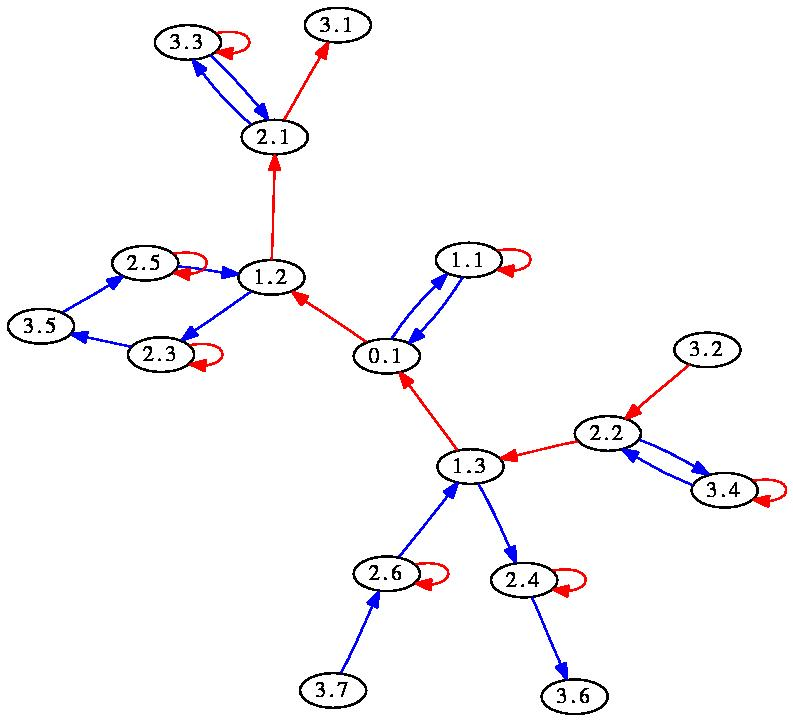
\includegraphics[height=5cm,keepaspectratio=true]{basilica-ball.jpg}   }

 }

 
\section{\textcolor{Chapter }{Finding short relations}}\logpage{[ 12, 4, 0 ]}
\hyperdef{L}{X791D4D398201C17D}{}
{
 

\subsection{\textcolor{Chapter }{ShortGroupRelations}}
\logpage{[ 12, 4, 1 ]}\nobreak
\hyperdef{L}{X868E478F86A10CFF}{}
{\noindent\textcolor{FuncColor}{$\triangleright$\ \ \texttt{ShortGroupRelations({\mdseries\slshape g, n})\index{ShortGroupRelations@\texttt{ShortGroupRelations}}
\label{ShortGroupRelations}
}\hfill{\scriptsize (operation)}}\\
\noindent\textcolor{FuncColor}{$\triangleright$\ \ \texttt{ShortMonoidRelations({\mdseries\slshape g, n})\index{ShortMonoidRelations@\texttt{ShortMonoidRelations}}
\label{ShortMonoidRelations}
}\hfill{\scriptsize (operation)}}\\
\textbf{\indent Returns:\ }
A list of relations between words over \mbox{\texttt{\mdseries\slshape g}}, of length at most \mbox{\texttt{\mdseries\slshape n}}.



 This function assumes that \mbox{\texttt{\mdseries\slshape g}} is a list of monoid elements. it searches for products of at most \mbox{\texttt{\mdseries\slshape n}} elements over \mbox{\texttt{\mdseries\slshape g}} that are equal. 

 In its first form, it returns a list of words in a free group \texttt{f} of rank the length of \mbox{\texttt{\mdseries\slshape g}}, that are trivial in \mbox{\texttt{\mdseries\slshape g}}. The first argument may be a group, in which case its symmetric generating
set is considered. 

 In its second form, it returns a list of pairs \texttt{[l,r]}, where \texttt{l} and \texttt{r} are words in a free monoid \texttt{f} of rank the length of \mbox{\texttt{\mdseries\slshape g}}, that are equal in \mbox{\texttt{\mdseries\slshape g}}. The first argument may be a monoid, in which case its monoid generating set
is considered. 

 This command does not construct all such pairs; rather, it returns a small
set, in the hope that it may serve as a presentation for the monoid generated
by \mbox{\texttt{\mdseries\slshape g}}. 

 The first element of the list returned is actually not a relation: it is a
homomorphism from \texttt{f} to [the group/monoid generated by] \mbox{\texttt{\mdseries\slshape g}}. 
\begin{Verbatim}[commandchars=!@|,fontsize=\small,frame=single,label=Example]
  !gapprompt@gap>| !gapinput@ShortGroupRelations(GrigorchukGroup,10);|
  [ [ x1, x2, x3, x4 ] -> [ a, b, c, d ],
    x1^2, x2^2, x3^2, x4^2, x2*x3*x4, x4*x1*x4*x1*x4*x1*x4*x1,
    x3*x1*x3*x1*x3*x1*x3*x1*x3*x1*x3*x1*x3*x1*x3*x1 ]
  !gapprompt@gap>| !gapinput@ShortGroupRelations(GuptaSidkiGroup,9);|
  [ [ x1, x2 ] -> [ x, gamma ],
    x1^3, x2^3, x2*x1^-1*x2*x1^-1*x2*x1^-1*x2*x1^-1*x2*x1^-1*x2*x1^-1*
       x2*x1^-1*x2*x1^-1*x2*x1^-1,    x1^-1*x2^-1*x1^-1*x2^-1*x1^-1*x2^-1*
  x1^-1*x2^-1*x1^-1*x2^-1*x1^-1*x2^-1*x1^-1*x2^-1*x1^-1*x2^-1*x1^-1*x2^-1 ]
\end{Verbatim}
 }

 

\subsection{\textcolor{Chapter }{ShortGroupWordInSet}}
\logpage{[ 12, 4, 2 ]}\nobreak
\hyperdef{L}{X7B9942AA84B0753E}{}
{\noindent\textcolor{FuncColor}{$\triangleright$\ \ \texttt{ShortGroupWordInSet({\mdseries\slshape g, s, n})\index{ShortGroupWordInSet@\texttt{ShortGroupWordInSet}}
\label{ShortGroupWordInSet}
}\hfill{\scriptsize (operation)}}\\
\noindent\textcolor{FuncColor}{$\triangleright$\ \ \texttt{ShortMonoidWordInSet({\mdseries\slshape g, s, n})\index{ShortMonoidWordInSet@\texttt{ShortMonoidWordInSet}}
\label{ShortMonoidWordInSet}
}\hfill{\scriptsize (operation)}}\\
\noindent\textcolor{FuncColor}{$\triangleright$\ \ \texttt{ShortSemigroupWordInSet({\mdseries\slshape g, s, n})\index{ShortSemigroupWordInSet@\texttt{ShortSemigroupWordInSet}}
\label{ShortSemigroupWordInSet}
}\hfill{\scriptsize (operation)}}\\
\textbf{\indent Returns:\ }
Words over \mbox{\texttt{\mdseries\slshape g}} that express elements of \mbox{\texttt{\mdseries\slshape s}}.



 This command produces words in the free group/monoid/semigroup generated by \mbox{\texttt{\mdseries\slshape g}}'s generators that express elements of the set \mbox{\texttt{\mdseries\slshape s}}. Elements of length at most \mbox{\texttt{\mdseries\slshape AbsoluteValue(n)}} are searched; if \mbox{\texttt{\mdseries\slshape n}} is non-negative then at most one element is returned. The value \texttt{\mbox{\texttt{\mdseries\slshape n}}=infinity} is allowed. 

 The second argument may be either a list, a predicate (i.e. a function
returning \texttt{true} or \texttt{false}) or an element. 

 The function returns a list of words in the free group/monoid/semigroup; the
first entry of the list is a homomorphism from the free group/monoid/semigroup
to \mbox{\texttt{\mdseries\slshape g}}. 
\begin{Verbatim}[commandchars=!@|,fontsize=\small,frame=single,label=Example]
  !gapprompt@gap>| !gapinput@l := ShortMonoidWordInSet(Group((1,2),(2,3),(3,4)),|
              [(1,2,3,4),(4,3,2,1)],-3);
  [ MappingByFunction( <free monoid on the generators [ m1, m2, m3 ]>, Group(
      [ (1,2), (2,3), (3,4) ]), function( w ) ... end ), m3*m2*m1, m1*m2*m3 ]
  !gapprompt@gap>| !gapinput@f := Remove(l,1);;|
  !gapprompt@gap>| !gapinput@List(l,x->x^f);|
  [ (1,2,3,4), (1,4,3,2) ]
  !gapprompt@gap>| !gapinput@ShortMonoidWordInSet(GrigorchukGroup,|
         [Comm(GrigorchukGroup.1,GrigorchukGroup.2)],4);
  [ MappingByFunction( <free monoid on the generators [ m1, m2, m3, m4
       ]>, <self-similar monoid over [ 1 .. 2 ] with
      4 generators>, function( w ) ... end ), m1*m2*m1*m2 ]
\end{Verbatim}
 }

 }

 
\section{\textcolor{Chapter }{Braid groups}}\logpage{[ 12, 5, 0 ]}
\hyperdef{L}{X82712E6C815DB9B2}{}
{
 

\subsection{\textcolor{Chapter }{SurfaceBraidFpGroup}}
\logpage{[ 12, 5, 1 ]}\nobreak
\hyperdef{L}{X84472A637B648C47}{}
{\noindent\textcolor{FuncColor}{$\triangleright$\ \ \texttt{SurfaceBraidFpGroup({\mdseries\slshape n, g, p})\index{SurfaceBraidFpGroup@\texttt{SurfaceBraidFpGroup}}
\label{SurfaceBraidFpGroup}
}\hfill{\scriptsize (function)}}\\
\noindent\textcolor{FuncColor}{$\triangleright$\ \ \texttt{PureSurfaceBraidFpGroup({\mdseries\slshape n, g, p})\index{PureSurfaceBraidFpGroup@\texttt{PureSurfaceBraidFpGroup}}
\label{PureSurfaceBraidFpGroup}
}\hfill{\scriptsize (function)}}\\
\textbf{\indent Returns:\ }
The [pure] surface braid group on \mbox{\texttt{\mdseries\slshape n}} strands.



 This function creates a finitely presented group, isomorphic to the [pure]
braid group on \mbox{\texttt{\mdseries\slshape n}} strands of the surface of genus \mbox{\texttt{\mdseries\slshape g}}, with \mbox{\texttt{\mdseries\slshape p}} punctures. In particular, \texttt{SurfaceBraidFpGroup(n,0,1)} is the usual braid group (on the disc). 

 The presentation comes from \cite{MR2043362}. The first $2g$ generators are the standard $a_i,b_i$ surface generators; the next $n-1$ are the standard $s_i$ braid generators; and the last are the extra $z$ generators. 

 The pure surface braid group is the kernel of the natural map from the surface
braid group to the symmetric group on \mbox{\texttt{\mdseries\slshape n}} points, defined by sending $a_i,b_i,z$ to the identity and $s_i$ to the transposition \texttt{(i,i+1)}. }

 

\subsection{\textcolor{Chapter }{CharneyBraidFpGroup}}
\logpage{[ 12, 5, 2 ]}\nobreak
\hyperdef{L}{X87E12292861FFE79}{}
{\noindent\textcolor{FuncColor}{$\triangleright$\ \ \texttt{CharneyBraidFpGroup({\mdseries\slshape n})\index{CharneyBraidFpGroup@\texttt{CharneyBraidFpGroup}}
\label{CharneyBraidFpGroup}
}\hfill{\scriptsize (function)}}\\
\textbf{\indent Returns:\ }
The braid group on \mbox{\texttt{\mdseries\slshape n}} strands.



 This function creates a finitely presented group, isomorphic to the braid
group on \mbox{\texttt{\mdseries\slshape n}} strands (on the disc). It is isomorphic to \texttt{SurfaceBraidFpGroup(n,0,1)}, but has a different presentation, due to Charney (\cite{MR1314589}), with one generator per non-trivial permutation of \mbox{\texttt{\mdseries\slshape n}} points. }

 

\subsection{\textcolor{Chapter }{ArtinRepresentation}}
\logpage{[ 12, 5, 3 ]}\nobreak
\hyperdef{L}{X814375977D2E4AD9}{}
{\noindent\textcolor{FuncColor}{$\triangleright$\ \ \texttt{ArtinRepresentation({\mdseries\slshape n})\index{ArtinRepresentation@\texttt{ArtinRepresentation}}
\label{ArtinRepresentation}
}\hfill{\scriptsize (function)}}\\
\textbf{\indent Returns:\ }
The braid group's representation on \texttt{FreeGroup(n)}.



 This function creates a Artin's representatin, a homomorphism from the braid
group on \mbox{\texttt{\mdseries\slshape n}} strands (on the disc) into the automorphism group of a free group of rank \mbox{\texttt{\mdseries\slshape n}}. }

 }

 
\section{\textcolor{Chapter }{Transformations on the integers}}\logpage{[ 12, 6, 0 ]}
\hyperdef{L}{X862138E9831375D1}{}
{
 

\subsection{\textcolor{Chapter }{TRANS{\textunderscore}FAMILY}}
\logpage{[ 12, 6, 1 ]}\nobreak
\hyperdef{L}{X7998343C85D9028B}{}
{\noindent\textcolor{FuncColor}{$\triangleright$\ \ \texttt{TRANS{\textunderscore}FAMILY\index{TRANSFAMILY@\texttt{TRANS{\textunderscore}FAMILY}}
\label{TRANSFAMILY}
}\hfill{\scriptsize (family)}}\\
\noindent\textcolor{FuncColor}{$\triangleright$\ \ \texttt{IsTrans\index{IsTrans@\texttt{IsTrans}}
\label{IsTrans}
}\hfill{\scriptsize (filter)}}\\


 The family and filter of transformations of the FR's implementation of
transformations on the positive integers, see \texttt{Trans} (\ref{Trans}). }

 

\subsection{\textcolor{Chapter }{Trans}}
\logpage{[ 12, 6, 2 ]}\nobreak
\hyperdef{L}{X7CA512F481AADD38}{}
{\noindent\textcolor{FuncColor}{$\triangleright$\ \ \texttt{Trans({\mdseries\slshape list, ...})\index{Trans@\texttt{Trans}}
\label{Trans}
}\hfill{\scriptsize (function)}}\\
\noindent\textcolor{FuncColor}{$\triangleright$\ \ \texttt{TransList({\mdseries\slshape list, ...})\index{TransList@\texttt{TransList}}
\label{TransList}
}\hfill{\scriptsize (function)}}\\
\noindent\textcolor{FuncColor}{$\triangleright$\ \ \texttt{TransNC({\mdseries\slshape list})\index{TransNC@\texttt{TransNC}}
\label{TransNC}
}\hfill{\scriptsize (function)}}\\


 This function creates a new transformation, in the family \texttt{TRANS{\textunderscore}FAMILY}. These objects behave quite as usual transformations (see \texttt{Transformation} (\textbf{Reference: Transformation})); the differences are that these transformations do not have a bounded set on
which they operate; they are all part of one family, and act on \texttt{PosInt}. The other difference is that, when they are invertible, these
transformations are simply permutations. 

 If one argument is passed, it is a list of images, as in \texttt{PermList} (\textbf{Reference: PermList}). If two arguments are passed and both are lists, they are the source and
range, as in \texttt{PermListList} (\textbf{Reference: PermListList}). Finally, if two arguments are passed and the second is a function, the first
argument is treated as the source and the range is computed with this
function. 

 Transformations are printed, and converted to strings, as \texttt{"{\textless}x,y,...{\textgreater}"}, where the \texttt{x,y,...} denote the images of \texttt{1,2,...} under the transformation; the shortest possible list is printed. 
\begin{Verbatim}[commandchars=!@|,fontsize=\small,frame=single,label=Example]
  !gapprompt@gap>| !gapinput@Trans();|
  <>
  !gapprompt@gap>| !gapinput@Trans([1,,2]);|
  <1,2,2>
  !gapprompt@gap>| !gapinput@3^last;|
  2
  !gapprompt@gap>| !gapinput@Trans([1,3,3]);|
  <1,3>
  !gapprompt@gap>| !gapinput@Trans([10,11],[11,12]);|
  <1,2,3,4,5,6,7,8,9,11,12>
  !gapprompt@gap>| !gapinput@Trans([10,11],x->x^2);|
  <1,2,3,4,5,6,7,8,9,100,121>
\end{Verbatim}
 }

 

\subsection{\textcolor{Chapter }{AsTrans}}
\logpage{[ 12, 6, 3 ]}\nobreak
\hyperdef{L}{X7BD9525684CA4DDF}{}
{\noindent\textcolor{FuncColor}{$\triangleright$\ \ \texttt{AsTrans({\mdseries\slshape perm})\index{AsTrans@\texttt{AsTrans}}
\label{AsTrans}
}\hfill{\scriptsize (operation)}}\\
\textbf{\indent Returns:\ }
An FR transformation equivalent to \mbox{\texttt{\mdseries\slshape perm}}.

}

 

\subsection{\textcolor{Chapter }{Cycle}}
\logpage{[ 12, 6, 4 ]}\nobreak
\hyperdef{L}{X80AF6E0683CA7F14}{}
{\noindent\textcolor{FuncColor}{$\triangleright$\ \ \texttt{Cycle({\mdseries\slshape trans, point})\index{Cycle@\texttt{Cycle}}
\label{Cycle}
}\hfill{\scriptsize (operation)}}\\
\textbf{\indent Returns:\ }
The cycle of integers that \mbox{\texttt{\mdseries\slshape point}} eventually reaches under \mbox{\texttt{\mdseries\slshape trans}}.

}

 

\subsection{\textcolor{Chapter }{Cycles}}
\logpage{[ 12, 6, 5 ]}\nobreak
\hyperdef{L}{X7F3B387A7FD8AE5E}{}
{\noindent\textcolor{FuncColor}{$\triangleright$\ \ \texttt{Cycles({\mdseries\slshape trans, domain[, act]})\index{Cycles@\texttt{Cycles}}
\label{Cycles}
}\hfill{\scriptsize (operation)}}\\
\textbf{\indent Returns:\ }
The cycles that \mbox{\texttt{\mdseries\slshape domain}} eventually reaches under \mbox{\texttt{\mdseries\slshape trans}}.

}

 

\subsection{\textcolor{Chapter }{FullTransMonoid}}
\logpage{[ 12, 6, 6 ]}\nobreak
\hyperdef{L}{X7A0C270587971BC5}{}
{\noindent\textcolor{FuncColor}{$\triangleright$\ \ \texttt{FullTransMonoid({\mdseries\slshape n})\index{FullTransMonoid@\texttt{FullTransMonoid}}
\label{FullTransMonoid}
}\hfill{\scriptsize (operation)}}\\
\textbf{\indent Returns:\ }
The monoid of transformations of \texttt{[1..n]} (if \mbox{\texttt{\mdseries\slshape n}} is an integer) or of \mbox{\texttt{\mdseries\slshape n}} (if \mbox{\texttt{\mdseries\slshape n}} is a collection).

}

 

\subsection{\textcolor{Chapter }{ImageSetOfTrans}}
\logpage{[ 12, 6, 7 ]}\nobreak
\hyperdef{L}{X7A6782FF84D7DD6E}{}
{\noindent\textcolor{FuncColor}{$\triangleright$\ \ \texttt{ImageSetOfTrans({\mdseries\slshape trans, coll})\index{ImageSetOfTrans@\texttt{ImageSetOfTrans}}
\label{ImageSetOfTrans}
}\hfill{\scriptsize (operation)}}\\
\textbf{\indent Returns:\ }
The images of \mbox{\texttt{\mdseries\slshape coll}} under \mbox{\texttt{\mdseries\slshape trans}}.

}

 

\subsection{\textcolor{Chapter }{KernelOfTrans}}
\logpage{[ 12, 6, 8 ]}\nobreak
\hyperdef{L}{X83C12D0A78B55A18}{}
{\noindent\textcolor{FuncColor}{$\triangleright$\ \ \texttt{KernelOfTrans({\mdseries\slshape trans})\index{KernelOfTrans@\texttt{KernelOfTrans}}
\label{KernelOfTrans}
}\hfill{\scriptsize (operation)}}\\
\textbf{\indent Returns:\ }
The non-trivial equivalence classes of integers identified under \mbox{\texttt{\mdseries\slshape trans}}.

}

 

\subsection{\textcolor{Chapter }{ListTrans}}
\logpage{[ 12, 6, 9 ]}\nobreak
\hyperdef{L}{X844C31CB7E3E7450}{}
{\noindent\textcolor{FuncColor}{$\triangleright$\ \ \texttt{ListTrans({\mdseries\slshape trans})\index{ListTrans@\texttt{ListTrans}}
\label{ListTrans}
}\hfill{\scriptsize (operation)}}\\
\textbf{\indent Returns:\ }
A list of images describing \mbox{\texttt{\mdseries\slshape trans}}.

}

 

\subsection{\textcolor{Chapter }{OneTrans}}
\logpage{[ 12, 6, 10 ]}\nobreak
\hyperdef{L}{X7860325178FA51D8}{}
{\noindent\textcolor{FuncColor}{$\triangleright$\ \ \texttt{OneTrans\index{OneTrans@\texttt{OneTrans}}
\label{OneTrans}
}\hfill{\scriptsize (global variable)}}\\


The identity FR transformation.}

 

\subsection{\textcolor{Chapter }{PreImagesOfTrans}}
\logpage{[ 12, 6, 11 ]}\nobreak
\hyperdef{L}{X7A3747D17B36F17E}{}
{\noindent\textcolor{FuncColor}{$\triangleright$\ \ \texttt{PreImagesOfTrans({\mdseries\slshape trans, i})\index{PreImagesOfTrans@\texttt{PreImagesOfTrans}}
\label{PreImagesOfTrans}
}\hfill{\scriptsize (operation)}}\\
\textbf{\indent Returns:\ }
The preimages of \mbox{\texttt{\mdseries\slshape i}} under \mbox{\texttt{\mdseries\slshape trans}}.

}

 

\subsection{\textcolor{Chapter }{RandomTrans}}
\logpage{[ 12, 6, 12 ]}\nobreak
\hyperdef{L}{X79A545B1833E425A}{}
{\noindent\textcolor{FuncColor}{$\triangleright$\ \ \texttt{RandomTrans({\mdseries\slshape n})\index{RandomTrans@\texttt{RandomTrans}}
\label{RandomTrans}
}\hfill{\scriptsize (operation)}}\\
\textbf{\indent Returns:\ }
A random FR transformation on the fist \mbox{\texttt{\mdseries\slshape n}} positive integers.

}

 

\subsection{\textcolor{Chapter }{RankOfTrans}}
\logpage{[ 12, 6, 13 ]}\nobreak
\hyperdef{L}{X829B3B9780140C53}{}
{\noindent\textcolor{FuncColor}{$\triangleright$\ \ \texttt{RankOfTrans({\mdseries\slshape trans[, list]})\index{RankOfTrans@\texttt{RankOfTrans}}
\label{RankOfTrans}
}\hfill{\scriptsize (function)}}\\
\textbf{\indent Returns:\ }
The (normalized) rank of the FR transformation \mbox{\texttt{\mdseries\slshape trans}}.



 If \mbox{\texttt{\mdseries\slshape list}} is present, this computes the size of the image of \mbox{\texttt{\mdseries\slshape list}} under \mbox{\texttt{\mdseries\slshape trans}}. Otherwise, this computes the limit, as $n\to\infty$, of \texttt{RankOfTrans(trans,[1..n])-n}. 
\begin{Verbatim}[commandchars=!@|,fontsize=\small,frame=single,label=Example]
  !gapprompt@gap>| !gapinput@RankOfTrans(Trans([1,1]));|
  !gapprompt@gap>| !gapinput@RankOfTrans(Trans([1,1]),[1..10]);|
  9
  -1
  !gapprompt@gap>| !gapinput@RankOfTrans(Trans());|
  0
\end{Verbatim}
 }

 

\subsection{\textcolor{Chapter }{RestrictedTrans}}
\logpage{[ 12, 6, 14 ]}\nobreak
\hyperdef{L}{X78D896347D0491F9}{}
{\noindent\textcolor{FuncColor}{$\triangleright$\ \ \texttt{RestrictedTrans({\mdseries\slshape trans, coll})\index{RestrictedTrans@\texttt{RestrictedTrans}}
\label{RestrictedTrans}
}\hfill{\scriptsize (operation)}}\\
\textbf{\indent Returns:\ }
The FR transformation that agrees with \mbox{\texttt{\mdseries\slshape trans}} on \mbox{\texttt{\mdseries\slshape coll}}, and is the identity elsewhere.

}

 }

 
\section{\textcolor{Chapter }{Complex numbers}}\logpage{[ 12, 7, 0 ]}
\hyperdef{L}{X7E09F9097DA0FB63}{}
{
 

\subsection{\textcolor{Chapter }{IsPMComplex}}
\logpage{[ 12, 7, 1 ]}\nobreak
\hyperdef{L}{X87EFAAE97B81054E}{}
{\noindent\textcolor{FuncColor}{$\triangleright$\ \ \texttt{IsPMComplex\index{IsPMComplex@\texttt{IsPMComplex}}
\label{IsPMComplex}
}\hfill{\scriptsize (filter)}}\\
\noindent\textcolor{FuncColor}{$\triangleright$\ \ \texttt{PMCOMPLEX{\textunderscore}FAMILY\index{PMCOMPLEXFAMILY@\texttt{PMCOMPLEX{\textunderscore}FAMILY}}
\label{PMCOMPLEXFAMILY}
}\hfill{\scriptsize (family)}}\\
\noindent\textcolor{FuncColor}{$\triangleright$\ \ \texttt{PMCOMPLEX{\textunderscore}PSEUDOFIELD\index{PMCOMPLEXPSEUDOFIELD@\texttt{PMC}\-\texttt{O}\-\texttt{M}\-\texttt{P}\-\texttt{L}\-\texttt{E}\-\texttt{X{\textunderscore}}\-\texttt{P}\-\texttt{S}\-\texttt{E}\-\texttt{U}\-\texttt{D}\-\texttt{O}\-\texttt{F}\-\texttt{IELD}}
\label{PMCOMPLEXPSEUDOFIELD}
}\hfill{\scriptsize (global variable)}}\\
\noindent\textcolor{FuncColor}{$\triangleright$\ \ \texttt{PMCOMPLEX\index{PMCOMPLEX@\texttt{PMCOMPLEX}}
\label{PMCOMPLEX}
}\hfill{\scriptsize (global variable)}}\\


 A "poor man's" implementation of complex numbers, based on the underlying
64-bit floating-point numbers in \textsf{GAP}. 

 Strictly speaking, complex numbers do not form a field in \textsf{GAP}, because associativity etc. do not hold. Still, a field is defined, \texttt{PMCOMPLEX{\textunderscore}FIELD}, making it possible to construct an indeterminate and rational functions, to
be passed to \textsf{FR}'s routines. 

 These complex numbers can be made the default floating-point numbers via \texttt{SetFloats(PMCOMPLEX);}. They may then be entered as standard floating-point numbers, with the suffix \texttt{{\textunderscore}z}. 
\begin{Verbatim}[commandchars=!@|,fontsize=\small,frame=single,label=Example]
  !gapprompt@gap>| !gapinput@z := Indeterminate(PMCOMPLEX_FIELD,"z");|
  z
  !gapprompt@gap>| !gapinput@(z+1/2)^5/(z-1/2);|
  (z^5+2.5*z^4+2.5*z^3+1.25*z^2+0.3125*z+0.03125)/(z+(-0.5))
  !gapprompt@gap>| !gapinput@NewFloat(IsPMComplex,1,2);|
  1+2i
  !gapprompt@gap>| !gapinput@last^2;|
  -3+4i
  !gapprompt@gap>| !gapinput@RealPart(last);|
  -3
  !gapprompt@gap>| !gapinput@Norm(last2);|
  25
  !gapprompt@gap>| !gapinput@NewFloat(IsPMComplex,"1+2*I");|
  1+2i
  !gapprompt@gap>| !gapinput@RootsFloat(z^2-5);|
  [ 2.23607, -2.23607 ]
  !gapprompt@gap>| !gapinput@RootsFloat(ListWithIdenticalEntries(80,1.0_z));|
  [ 0.987688+0.156434i, 0.996917+0.0784591i, 0.996917-0.0784591i, 0.987688-0.156434i, 0.760406+0.649448i, 0.92388+0.382683i, 0.951057-0.309017i, 0.97237+0.233445i, 0.809017+0.587785i,
    0.522499+0.85264i, 0.649448+0.760406i, 0.891007+0.45399i, 0.587785+0.809017i, 0.707107+0.707107i, 0.951057+0.309017i, 0.233445+0.97237i, 0.45399+0.891007i, 0.309017+0.951057i,
    0.382683+0.92388i, 0.85264+0.522499i, -0.59719-0.608203i, -0.867574-0.11552i, -0.186972-0.990223i, -0.999006+0.318176i, -0.739308+0.0272973i, -0.432752-0.7287i, -0.672709+0.537561i,
    0.156434+0.987688i, 0.295424-0.953359i, 0.588289-0.808509i, 0.455128-0.893999i, 0.0951213-1.01063i, 0.229628-0.939435i, -0.216054-0.95336i, -0.914152+0.49378i, 0.524052-0.853005i,
    0.97237-0.233445i, -0.233486+0.972416i, 0.379514-0.92918i, 3.09131e-07+1.i, 0.182752-0.984684i, 0.891007-0.45399i, -0.0892207-1.01443i, 0.852641-0.522499i, 0.00247318-1.02032i,
    0.92388-0.382683i, -0.585832+0.81608i, 0.809018-0.587792i, -0.656055+0.770506i, 0.760385-0.649467i, -0.452862+0.889692i, -0.0784562+0.996918i, 0.707015-0.707079i, 0.0784591+0.996917i,
    -0.15643+0.987703i, -0.307608-0.969002i, 0.649377-0.760134i, -0.382904+0.92328i, -0.857704+0.573345i, -0.403754-0.946275i, -0.827986-0.648221i, -0.990655-0.396897i,
    -0.929824-0.488558i, -0.671579-0.790133i, -0.886052-0.560249i, -1.05047-0.0873829i, -0.496236-0.900246i, -0.726008+0.713809i, -1.02514+0.223541i, -1.01722-0.277614i,
    -0.585809-0.852796i, -0.518635+0.85364i, -1.04842+0.0255453i, -0.752485-0.724528i, -0.309225+0.951018i, -0.9612+0.409487i, -0.793651+0.646744i, -1.01735-0.194111i, -1.04161+0.124175i
   ]
  !gapprompt@gap>| !gapinput@AsSortedList(List(last,AbsoluteValue));|
  [ 0.739812, 0.847513, 0.852377, 0.861109, 0.875231, 0.967092, 0.977534, 0.998083, 0.998317, 0.998841, 0.99953, 0.999747, 0.999886, 0.999916, 0.999996, 1., 1., 1., 1., 1., 1., 1., 1.,
    1., 1., 1., 1., 1., 1., 1., 1., 1., 1., 1., 1., 1., 1., 1., 1., 1., 1., 1., 1., 1.00001, 1.00001, 1.00003, 1.00005, 1.00112, 1.0015, 1.00318, 1.0037, 1.00458, 1.00772, 1.01197,
    1.01509, 1.01665, 1.01814, 1.01834, 1.02033, 1.0238, 1.02796, 1.02881, 1.03169, 1.03462, 1.0357, 1.03698, 1.03899, 1.04459, 1.04479, 1.04832, 1.04845, 1.04873, 1.04899, 1.04923,
    1.05036, 1.05155, 1.0541, 1.05442, 1.0672 ]
  
\end{Verbatim}
 }

 }

 
\section{\textcolor{Chapter }{P1 points}}\logpage{[ 12, 8, 0 ]}
\hyperdef{L}{X82A013F78010EC06}{}
{
 

\subsection{\textcolor{Chapter }{IsP1Point}}
\logpage{[ 12, 8, 1 ]}\nobreak
\hyperdef{L}{X84AD618C7906AC92}{}
{\noindent\textcolor{FuncColor}{$\triangleright$\ \ \texttt{IsP1Point\index{IsP1Point@\texttt{IsP1Point}}
\label{IsP1Point}
}\hfill{\scriptsize (filter)}}\\
\noindent\textcolor{FuncColor}{$\triangleright$\ \ \texttt{P1PointsFamily\index{P1PointsFamily@\texttt{P1PointsFamily}}
\label{P1PointsFamily}
}\hfill{\scriptsize (family)}}\\
\noindent\textcolor{FuncColor}{$\triangleright$\ \ \texttt{P1Point({\mdseries\slshape complex})\index{P1Point@\texttt{P1Point}}
\label{P1Point}
}\hfill{\scriptsize (function)}}\\
\noindent\textcolor{FuncColor}{$\triangleright$\ \ \texttt{P1Point({\mdseries\slshape real, imag})\index{P1Point@\texttt{P1Point}!ri}
\label{P1Point:ri}
}\hfill{\scriptsize (function)}}\\
\noindent\textcolor{FuncColor}{$\triangleright$\ \ \texttt{P1Point({\mdseries\slshape string})\index{P1Point@\texttt{P1Point}!s}
\label{P1Point:s}
}\hfill{\scriptsize (function)}}\\


 P1 points are complex numbers or infinity; fast methods are implemented to
compute with them, and to apply rational maps to them. 

 The first filter recognizes these objects. Next, the family they belong to.
The next methods create a new P1 point. }

 

\subsection{\textcolor{Chapter }{CleanedP1Point}}
\logpage{[ 12, 8, 2 ]}\nobreak
\hyperdef{L}{X80B00F0685209993}{}
{\noindent\textcolor{FuncColor}{$\triangleright$\ \ \texttt{CleanedP1Point({\mdseries\slshape p, prec})\index{CleanedP1Point@\texttt{CleanedP1Point}}
\label{CleanedP1Point}
}\hfill{\scriptsize (function)}}\\
\textbf{\indent Returns:\ }
\mbox{\texttt{\mdseries\slshape p}}, rounded towards 0/1/infinity/reals at precision \mbox{\texttt{\mdseries\slshape prec}}.

}

 

\subsection{\textcolor{Chapter }{P1infinity}}
\logpage{[ 12, 8, 3 ]}\nobreak
\hyperdef{L}{X87AC40C579500473}{}
{\noindent\textcolor{FuncColor}{$\triangleright$\ \ \texttt{P1infinity\index{P1infinity@\texttt{P1infinity}}
\label{P1infinity}
}\hfill{\scriptsize (global variable)}}\\
\noindent\textcolor{FuncColor}{$\triangleright$\ \ \texttt{P1one\index{P1one@\texttt{P1one}}
\label{P1one}
}\hfill{\scriptsize (global variable)}}\\
\noindent\textcolor{FuncColor}{$\triangleright$\ \ \texttt{P1zero\index{P1zero@\texttt{P1zero}}
\label{P1zero}
}\hfill{\scriptsize (global variable)}}\\


The south, north and 'east' poles of the Riemann sphere.}

 

\subsection{\textcolor{Chapter }{P1Antipode}}
\logpage{[ 12, 8, 4 ]}\nobreak
\hyperdef{L}{X80DB7A677E1EF1F6}{}
{\noindent\textcolor{FuncColor}{$\triangleright$\ \ \texttt{P1Antipode({\mdseries\slshape p})\index{P1Antipode@\texttt{P1Antipode}}
\label{P1Antipode}
}\hfill{\scriptsize (function)}}\\
\textbf{\indent Returns:\ }
The antipode of \mbox{\texttt{\mdseries\slshape p}} on the Riemann sphere.

}

 

\subsection{\textcolor{Chapter }{P1Barycentre}}
\logpage{[ 12, 8, 5 ]}\nobreak
\hyperdef{L}{X7E220B497FF24C98}{}
{\noindent\textcolor{FuncColor}{$\triangleright$\ \ \texttt{P1Barycentre({\mdseries\slshape points, ...})\index{P1Barycentre@\texttt{P1Barycentre}}
\label{P1Barycentre}
}\hfill{\scriptsize (function)}}\\
\textbf{\indent Returns:\ }
The barycentre of its arguments (which can also be a list of P1 points).

}

 

\subsection{\textcolor{Chapter }{P1Circumcentre}}
\logpage{[ 12, 8, 6 ]}\nobreak
\hyperdef{L}{X83BD8B5C856DF570}{}
{\noindent\textcolor{FuncColor}{$\triangleright$\ \ \texttt{P1Circumcentre({\mdseries\slshape p, q, r})\index{P1Circumcentre@\texttt{P1Circumcentre}}
\label{P1Circumcentre}
}\hfill{\scriptsize (function)}}\\
\textbf{\indent Returns:\ }
The centre of the smallest disk containing \mbox{\texttt{\mdseries\slshape p,q,r}}.

}

 

\subsection{\textcolor{Chapter }{P1Distance}}
\logpage{[ 12, 8, 7 ]}\nobreak
\hyperdef{L}{X7A3A339181EF9D24}{}
{\noindent\textcolor{FuncColor}{$\triangleright$\ \ \texttt{P1Distance({\mdseries\slshape p, q})\index{P1Distance@\texttt{P1Distance}}
\label{P1Distance}
}\hfill{\scriptsize (function)}}\\
\textbf{\indent Returns:\ }
The spherical distance from \mbox{\texttt{\mdseries\slshape p}} to \mbox{\texttt{\mdseries\slshape q}}.

}

 

\subsection{\textcolor{Chapter }{P1Midpoint}}
\logpage{[ 12, 8, 8 ]}\nobreak
\hyperdef{L}{X86D3189D83BA09F8}{}
{\noindent\textcolor{FuncColor}{$\triangleright$\ \ \texttt{P1Midpoint({\mdseries\slshape p, q})\index{P1Midpoint@\texttt{P1Midpoint}}
\label{P1Midpoint}
}\hfill{\scriptsize (function)}}\\
\textbf{\indent Returns:\ }
The point between \mbox{\texttt{\mdseries\slshape p}} to \mbox{\texttt{\mdseries\slshape q}} (undefined if they are antipodes of each other).

}

 

\subsection{\textcolor{Chapter }{P1Sphere}}
\logpage{[ 12, 8, 9 ]}\nobreak
\hyperdef{L}{X7FC042FA8032C1A5}{}
{\noindent\textcolor{FuncColor}{$\triangleright$\ \ \texttt{P1Sphere({\mdseries\slshape v})\index{P1Sphere@\texttt{P1Sphere}}
\label{P1Sphere}
}\hfill{\scriptsize (function)}}\\
\textbf{\indent Returns:\ }
The P1 point corresponding to \mbox{\texttt{\mdseries\slshape v}} in $\mathbb R^3$.

}

 

\subsection{\textcolor{Chapter }{SphereP1}}
\logpage{[ 12, 8, 10 ]}\nobreak
\hyperdef{L}{X83072FCB86850BDA}{}
{\noindent\textcolor{FuncColor}{$\triangleright$\ \ \texttt{SphereP1({\mdseries\slshape p})\index{SphereP1@\texttt{SphereP1}}
\label{SphereP1}
}\hfill{\scriptsize (function)}}\\
\textbf{\indent Returns:\ }
The coordinates in $\mathbb R^3$ of \mbox{\texttt{\mdseries\slshape p}}.

}

 

\subsection{\textcolor{Chapter }{SphereP1Y}}
\logpage{[ 12, 8, 11 ]}\nobreak
\hyperdef{L}{X87B815958442BA68}{}
{\noindent\textcolor{FuncColor}{$\triangleright$\ \ \texttt{SphereP1Y({\mdseries\slshape p})\index{SphereP1Y@\texttt{SphereP1Y}}
\label{SphereP1Y}
}\hfill{\scriptsize (function)}}\\
\textbf{\indent Returns:\ }
The Y coordinate in $\mathbb R^3$ of \mbox{\texttt{\mdseries\slshape p}}.

}

 

\subsection{\textcolor{Chapter }{P1XRatio}}
\logpage{[ 12, 8, 12 ]}\nobreak
\hyperdef{L}{X7C50C284794F35A8}{}
{\noindent\textcolor{FuncColor}{$\triangleright$\ \ \texttt{P1XRatio({\mdseries\slshape p, q, r, s})\index{P1XRatio@\texttt{P1XRatio}}
\label{P1XRatio}
}\hfill{\scriptsize (function)}}\\
\textbf{\indent Returns:\ }
The cross ratio of \mbox{\texttt{\mdseries\slshape p, q, r, s}}.

}

 

\subsection{\textcolor{Chapter }{IsP1Map}}
\logpage{[ 12, 8, 13 ]}\nobreak
\hyperdef{L}{X7E5D08E07C9994F8}{}
{\noindent\textcolor{FuncColor}{$\triangleright$\ \ \texttt{IsP1Map\index{IsP1Map@\texttt{IsP1Map}}
\label{IsP1Map}
}\hfill{\scriptsize (filter)}}\\
\noindent\textcolor{FuncColor}{$\triangleright$\ \ \texttt{P1MapsFamily\index{P1MapsFamily@\texttt{P1MapsFamily}}
\label{P1MapsFamily}
}\hfill{\scriptsize (family)}}\\


 P1 maps are stored more efficiently than rational functions, but are otherwise
equivalent. 

 The first filter recognizes these objects. Next, the family they belong to. }

 

\subsection{\textcolor{Chapter }{MoebiusMap}}
\logpage{[ 12, 8, 14 ]}\nobreak
\hyperdef{L}{X83D5E52A7FFB797D}{}
{\noindent\textcolor{FuncColor}{$\triangleright$\ \ \texttt{MoebiusMap({\mdseries\slshape [sourcelist, ]destlist})\index{MoebiusMap@\texttt{MoebiusMap}}
\label{MoebiusMap}
}\hfill{\scriptsize (function)}}\\
\noindent\textcolor{FuncColor}{$\triangleright$\ \ \texttt{MoebiusMap({\mdseries\slshape p, q, r, s, t, u})\index{MoebiusMap@\texttt{MoebiusMap}!6}
\label{MoebiusMap:6}
}\hfill{\scriptsize (function)}}\\
\noindent\textcolor{FuncColor}{$\triangleright$\ \ \texttt{MoebiusMap({\mdseries\slshape p, q, r})\index{MoebiusMap@\texttt{MoebiusMap}!3}
\label{MoebiusMap:3}
}\hfill{\scriptsize (function)}}\\
\noindent\textcolor{FuncColor}{$\triangleright$\ \ \texttt{MoebiusMap({\mdseries\slshape p, q})\index{MoebiusMap@\texttt{MoebiusMap}!2}
\label{MoebiusMap:2}
}\hfill{\scriptsize (function)}}\\


 These methods create a new P1 map. In the first case, this is the M{\"o}bius
transformation sending \mbox{\texttt{\mdseries\slshape p,q,r}} to \mbox{\texttt{\mdseries\slshape P,Q,R}} respectively; in the second case, the map sending \mbox{\texttt{\mdseries\slshape p,q,r}} to \texttt{0,1,P1infinity} respectively; in the third case, the map sending \mbox{\texttt{\mdseries\slshape p,q}} to \texttt{0,P1infinity} respectively, of the form $(z-p)/(z-q)$. }

 

\subsection{\textcolor{Chapter }{P1z}}
\logpage{[ 12, 8, 15 ]}\nobreak
\hyperdef{L}{X7B5CBC0585889AC9}{}
{\noindent\textcolor{FuncColor}{$\triangleright$\ \ \texttt{P1z\index{P1z@\texttt{P1z}}
\label{P1z}
}\hfill{\scriptsize (global variable)}}\\


The identity M{\"o}bius transformation.}

 

\subsection{\textcolor{Chapter }{CleanedP1Map}}
\logpage{[ 12, 8, 16 ]}\nobreak
\hyperdef{L}{X87A94D82784C718C}{}
{\noindent\textcolor{FuncColor}{$\triangleright$\ \ \texttt{CleanedP1Map({\mdseries\slshape map, prec})\index{CleanedP1Map@\texttt{CleanedP1Map}}
\label{CleanedP1Map}
}\hfill{\scriptsize (operation)}}\\
\textbf{\indent Returns:\ }
\mbox{\texttt{\mdseries\slshape map}}, with coefficients rounded using \mbox{\texttt{\mdseries\slshape prec}}.

}

 

\subsection{\textcolor{Chapter }{CoefficientsOfP1Map}}
\logpage{[ 12, 8, 17 ]}\nobreak
\hyperdef{L}{X7AFFF43383BF5001}{}
{\noindent\textcolor{FuncColor}{$\triangleright$\ \ \texttt{CoefficientsOfP1Map({\mdseries\slshape map})\index{CoefficientsOfP1Map@\texttt{CoefficientsOfP1Map}}
\label{CoefficientsOfP1Map}
}\hfill{\scriptsize (operation)}}\\
\textbf{\indent Returns:\ }
Coefficients of numerator and denominator of \mbox{\texttt{\mdseries\slshape map}}, lowest degree first.

}

 

\subsection{\textcolor{Chapter }{P1MapByCoefficients}}
\logpage{[ 12, 8, 18 ]}\nobreak
\hyperdef{L}{X7DE9419F7E0FADE9}{}
{\noindent\textcolor{FuncColor}{$\triangleright$\ \ \texttt{P1MapByCoefficients({\mdseries\slshape numer, denom})\index{P1MapByCoefficients@\texttt{P1MapByCoefficients}}
\label{P1MapByCoefficients}
}\hfill{\scriptsize (operation)}}\\
\textbf{\indent Returns:\ }
The P1 map with numerator coefficients \mbox{\texttt{\mdseries\slshape numer}} and denominator \mbox{\texttt{\mdseries\slshape denom}}, lowest degree first.

}

 

\subsection{\textcolor{Chapter }{P1Path}}
\logpage{[ 12, 8, 19 ]}\nobreak
\hyperdef{L}{X78DBA65C7990FE8A}{}
{\noindent\textcolor{FuncColor}{$\triangleright$\ \ \texttt{P1Path({\mdseries\slshape p, q})\index{P1Path@\texttt{P1Path}}
\label{P1Path}
}\hfill{\scriptsize (operation)}}\\
\textbf{\indent Returns:\ }
The P1 map sending \texttt{0} to \mbox{\texttt{\mdseries\slshape p}} and \texttt{1} to \mbox{\texttt{\mdseries\slshape q}}.

}

 

\subsection{\textcolor{Chapter }{DegreeOfP1Map}}
\logpage{[ 12, 8, 20 ]}\nobreak
\hyperdef{L}{X78DB4F257D1E2E8B}{}
{\noindent\textcolor{FuncColor}{$\triangleright$\ \ \texttt{DegreeOfP1Map({\mdseries\slshape map})\index{DegreeOfP1Map@\texttt{DegreeOfP1Map}}
\label{DegreeOfP1Map}
}\hfill{\scriptsize (operation)}}\\
\textbf{\indent Returns:\ }
The degree of \mbox{\texttt{\mdseries\slshape map}}.

}

 

\subsection{\textcolor{Chapter }{P1Image}}
\logpage{[ 12, 8, 21 ]}\nobreak
\hyperdef{L}{X78BB00397DBDE5F5}{}
{\noindent\textcolor{FuncColor}{$\triangleright$\ \ \texttt{P1Image({\mdseries\slshape map, p1point})\index{P1Image@\texttt{P1Image}}
\label{P1Image}
}\hfill{\scriptsize (operation)}}\\
\textbf{\indent Returns:\ }
The image of \mbox{\texttt{\mdseries\slshape p1point}} under \mbox{\texttt{\mdseries\slshape map}}.

}

 

\subsection{\textcolor{Chapter }{P1PreImages}}
\logpage{[ 12, 8, 22 ]}\nobreak
\hyperdef{L}{X8523E70785E32A8F}{}
{\noindent\textcolor{FuncColor}{$\triangleright$\ \ \texttt{P1PreImages({\mdseries\slshape map, p1point})\index{P1PreImages@\texttt{P1PreImages}}
\label{P1PreImages}
}\hfill{\scriptsize (operation)}}\\
\textbf{\indent Returns:\ }
The preimages of \mbox{\texttt{\mdseries\slshape p1point}} under \mbox{\texttt{\mdseries\slshape map}}.

}

 

\subsection{\textcolor{Chapter }{P1MapCriticalPoints}}
\logpage{[ 12, 8, 23 ]}\nobreak
\hyperdef{L}{X78B3055980B23917}{}
{\noindent\textcolor{FuncColor}{$\triangleright$\ \ \texttt{P1MapCriticalPoints({\mdseries\slshape map})\index{P1MapCriticalPoints@\texttt{P1MapCriticalPoints}}
\label{P1MapCriticalPoints}
}\hfill{\scriptsize (operation)}}\\
\textbf{\indent Returns:\ }
The critical points of \mbox{\texttt{\mdseries\slshape map}}.

}

 

\subsection{\textcolor{Chapter }{P1MapRational}}
\logpage{[ 12, 8, 24 ]}\nobreak
\hyperdef{L}{X8362CB5B79247851}{}
{\noindent\textcolor{FuncColor}{$\triangleright$\ \ \texttt{P1MapRational({\mdseries\slshape rat})\index{P1MapRational@\texttt{P1MapRational}}
\label{P1MapRational}
}\hfill{\scriptsize (operation)}}\\
\textbf{\indent Returns:\ }
The P1 map given by the rational function \mbox{\texttt{\mdseries\slshape rat}}.

}

 

\subsection{\textcolor{Chapter }{RationalP1Map}}
\logpage{[ 12, 8, 25 ]}\nobreak
\hyperdef{L}{X84BEAA60839AADAA}{}
{\noindent\textcolor{FuncColor}{$\triangleright$\ \ \texttt{RationalP1Map({\mdseries\slshape map})\index{RationalP1Map@\texttt{RationalP1Map}}
\label{RationalP1Map}
}\hfill{\scriptsize (operation)}}\\
\noindent\textcolor{FuncColor}{$\triangleright$\ \ \texttt{RationalP1Map({\mdseries\slshape indeterminate, map})\index{RationalP1Map@\texttt{RationalP1Map}!im}
\label{RationalP1Map:im}
}\hfill{\scriptsize (operation)}}\\
\textbf{\indent Returns:\ }
The rational function given by P1 map \mbox{\texttt{\mdseries\slshape map}}.

}

 

\subsection{\textcolor{Chapter }{P1MapSL2}}
\logpage{[ 12, 8, 26 ]}\nobreak
\hyperdef{L}{X83410A948102C845}{}
{\noindent\textcolor{FuncColor}{$\triangleright$\ \ \texttt{P1MapSL2({\mdseries\slshape mat})\index{P1MapSL2@\texttt{P1MapSL2}}
\label{P1MapSL2}
}\hfill{\scriptsize (operation)}}\\
\textbf{\indent Returns:\ }
The M{\"o}bius P1 map given by the 2x2 matrix \mbox{\texttt{\mdseries\slshape mat}}.

}

 

\subsection{\textcolor{Chapter }{SL2P1Map}}
\logpage{[ 12, 8, 27 ]}\nobreak
\hyperdef{L}{X840A9CD185F5519C}{}
{\noindent\textcolor{FuncColor}{$\triangleright$\ \ \texttt{SL2P1Map({\mdseries\slshape map})\index{SL2P1Map@\texttt{SL2P1Map}}
\label{SL2P1Map}
}\hfill{\scriptsize (operation)}}\\
\textbf{\indent Returns:\ }
The matrix of the M{\"o}bius P1 map \mbox{\texttt{\mdseries\slshape map}}.

}

 

\subsection{\textcolor{Chapter }{SetP1Points}}
\logpage{[ 12, 8, 28 ]}\nobreak
\hyperdef{L}{X874D59BD87D136D0}{}
{\noindent\textcolor{FuncColor}{$\triangleright$\ \ \texttt{SetP1Points({\mdseries\slshape record[, prec]})\index{SetP1Points@\texttt{SetP1Points}}
\label{SetP1Points}
}\hfill{\scriptsize (function)}}\\


 Installs a default implementation for P1 points. Fundamentally, a P1 point is
a complex number or infinity, with a few extra methods. The argument \mbox{\texttt{\mdseries\slshape record}} is the record describing the floating-point implementation. 

 Currently, one implementation (the default) is based on pairs of IEEE754
floateans. It is fast, but is limited to 53 bits of precision. It is loaded
via \texttt{SetP1Points(PMCOMPLEX);}. 

 Another implementation, in case the package \textsf{Float} is available, is based on MPC complex numbers. It offers unlimited precision,
but is much slower. It is loaded via \texttt{SetP1Points(MPC);} or \texttt{SetP1Points(MPC,prec);}. }

 }

 
\section{\textcolor{Chapter }{Dirichlet series}}\logpage{[ 12, 9, 0 ]}
\hyperdef{L}{X839ED1F982DB3469}{}
{
 

\subsection{\textcolor{Chapter }{DirichletSeries (0)}}
\logpage{[ 12, 9, 1 ]}\nobreak
\hyperdef{L}{X82D4E885838CFBD6}{}
{\noindent\textcolor{FuncColor}{$\triangleright$\ \ \texttt{DirichletSeries({\mdseries\slshape })\index{DirichletSeries@\texttt{DirichletSeries}!0}
\label{DirichletSeries:0}
}\hfill{\scriptsize (operation)}}\\
\noindent\textcolor{FuncColor}{$\triangleright$\ \ \texttt{DirichletSeries({\mdseries\slshape maxdeg})\index{DirichletSeries@\texttt{DirichletSeries}!md}
\label{DirichletSeries:md}
}\hfill{\scriptsize (operation)}}\\
\noindent\textcolor{FuncColor}{$\triangleright$\ \ \texttt{DirichletSeries({\mdseries\slshape indices, coeffs[, maxdeg]})\index{DirichletSeries@\texttt{DirichletSeries}!ic}
\label{DirichletSeries:ic}
}\hfill{\scriptsize (operation)}}\\
\noindent\textcolor{FuncColor}{$\triangleright$\ \ \texttt{DirichletSeries({\mdseries\slshape series, maxdeg})\index{DirichletSeries@\texttt{DirichletSeries}!sm}
\label{DirichletSeries:sm}
}\hfill{\scriptsize (operation)}}\\


 Creates a new Dirichlet series, namely, a formal power series of the form $f(s)=\sum_{n\ge1} a(n) n^{-s}$. Such series have a maximal degree, which may be \texttt{infinity}, and may be added or multiplied as polynomials. }

 

\subsection{\textcolor{Chapter }{DegreeDirichletSeries}}
\logpage{[ 12, 9, 2 ]}\nobreak
\hyperdef{L}{X7C8CD28D797A527F}{}
{\noindent\textcolor{FuncColor}{$\triangleright$\ \ \texttt{DegreeDirichletSeries({\mdseries\slshape f})\index{DegreeDirichletSeries@\texttt{DegreeDirichletSeries}}
\label{DegreeDirichletSeries}
}\hfill{\scriptsize (attribute)}}\\
\textbf{\indent Returns:\ }
The maximal degree of a non-zero coefficient of \mbox{\texttt{\mdseries\slshape f}}.

}

 

\subsection{\textcolor{Chapter }{SpreadDirichletSeries}}
\logpage{[ 12, 9, 3 ]}\nobreak
\hyperdef{L}{X81EA791C7CA3C3FF}{}
{\noindent\textcolor{FuncColor}{$\triangleright$\ \ \texttt{SpreadDirichletSeries({\mdseries\slshape f, n})\index{SpreadDirichletSeries@\texttt{SpreadDirichletSeries}}
\label{SpreadDirichletSeries}
}\hfill{\scriptsize (attribute)}}\\
\textbf{\indent Returns:\ }
The series $f(ns)$.

}

 

\subsection{\textcolor{Chapter }{ShiftDirichletSeries}}
\logpage{[ 12, 9, 4 ]}\nobreak
\hyperdef{L}{X7D792C6985BF482B}{}
{\noindent\textcolor{FuncColor}{$\triangleright$\ \ \texttt{ShiftDirichletSeries({\mdseries\slshape s, n})\index{ShiftDirichletSeries@\texttt{ShiftDirichletSeries}}
\label{ShiftDirichletSeries}
}\hfill{\scriptsize (attribute)}}\\
\textbf{\indent Returns:\ }
The series $n^{-s}f(s)$.

}

 

\subsection{\textcolor{Chapter }{ShrunkDirichletSeries}}
\logpage{[ 12, 9, 5 ]}\nobreak
\hyperdef{L}{X80571E4A86B38D53}{}
{\noindent\textcolor{FuncColor}{$\triangleright$\ \ \texttt{ShrunkDirichletSeries({\mdseries\slshape f})\index{ShrunkDirichletSeries@\texttt{ShrunkDirichletSeries}}
\label{ShrunkDirichletSeries}
}\hfill{\scriptsize (attribute)}}\\
\textbf{\indent Returns:\ }
The series \mbox{\texttt{\mdseries\slshape f}}, with maximal precision set to its maximal degree.

}

 

\subsection{\textcolor{Chapter }{ZetaSeriesOfGroup}}
\logpage{[ 12, 9, 6 ]}\nobreak
\hyperdef{L}{X850F072E8523EE9D}{}
{\noindent\textcolor{FuncColor}{$\triangleright$\ \ \texttt{ZetaSeriesOfGroup({\mdseries\slshape G})\index{ZetaSeriesOfGroup@\texttt{ZetaSeriesOfGroup}}
\label{ZetaSeriesOfGroup}
}\hfill{\scriptsize (attribute)}}\\
\textbf{\indent Returns:\ }
The series \mbox{\texttt{\mdseries\slshape \texttt{\symbol{92}}sum{\textunderscore}\texttt{\symbol{123}}\texttt{\symbol{92}}chi\texttt{\symbol{92}}in\texttt{\symbol{92}}widehat
G\texttt{\symbol{125}}(\texttt{\symbol{92}}dim
G)\texttt{\symbol{94}}\texttt{\symbol{123}}-s\texttt{\symbol{125}}}}.

}

 

\subsection{\textcolor{Chapter }{ValueOfDirichletSeries}}
\logpage{[ 12, 9, 7 ]}\nobreak
\hyperdef{L}{X7F49DDBC829F18C8}{}
{\noindent\textcolor{FuncColor}{$\triangleright$\ \ \texttt{ValueOfDirichletSeries({\mdseries\slshape f, s})\index{ValueOfDirichletSeries@\texttt{ValueOfDirichletSeries}}
\label{ValueOfDirichletSeries}
}\hfill{\scriptsize (attribute)}}\\
\textbf{\indent Returns:\ }
The evaluation of \mbox{\texttt{\mdseries\slshape f}} at \mbox{\texttt{\mdseries\slshape s}}. Synonym for \texttt{Value}.

}

 }

 
\section{\textcolor{Chapter }{Projective representations}}\logpage{[ 12, 10, 0 ]}
\hyperdef{L}{X86256BD187D9A7FF}{}
{
 

\subsection{\textcolor{Chapter }{IsProjectiveRepresentation}}
\logpage{[ 12, 10, 1 ]}\nobreak
\hyperdef{L}{X7CE116C27EF109D1}{}
{\noindent\textcolor{FuncColor}{$\triangleright$\ \ \texttt{IsProjectiveRepresentation({\mdseries\slshape rep})\index{IsProjectiveRepresentation@\texttt{IsProjectiveRepresentation}}
\label{IsProjectiveRepresentation}
}\hfill{\scriptsize (property)}}\\
\noindent\textcolor{FuncColor}{$\triangleright$\ \ \texttt{IsLinearRepresentation({\mdseries\slshape rep})\index{IsLinearRepresentation@\texttt{IsLinearRepresentation}}
\label{IsLinearRepresentation}
}\hfill{\scriptsize (property)}}\\


 A projective representation is a mapping to matrices, that is multiplicative
up to scalars. This property is set by the following functions that create
projective representations. 

 The second property describes those projective representations that are in
fact homomorphisms. }

 

\subsection{\textcolor{Chapter }{ProjectiveRepresentationByFunction}}
\logpage{[ 12, 10, 2 ]}\nobreak
\hyperdef{L}{X80EEB0F58467ED68}{}
{\noindent\textcolor{FuncColor}{$\triangleright$\ \ \texttt{ProjectiveRepresentationByFunction({\mdseries\slshape group, matrixgroup, function})\index{ProjectiveRepresentationByFunction@\texttt{ProjectiveRepresentationByFunction}}
\label{ProjectiveRepresentationByFunction}
}\hfill{\scriptsize (operation)}}\\
\textbf{\indent Returns:\ }
A projective representation of \mbox{\texttt{\mdseries\slshape group}}.

}

 

\subsection{\textcolor{Chapter }{LinearRepresentationByImages}}
\logpage{[ 12, 10, 3 ]}\nobreak
\hyperdef{L}{X7FC5A28278EB1E51}{}
{\noindent\textcolor{FuncColor}{$\triangleright$\ \ \texttt{LinearRepresentationByImages({\mdseries\slshape group, matrixgroup, src, dst})\index{LinearRepresentationByImages@\texttt{LinearRepresentationByImages}}
\label{LinearRepresentationByImages}
}\hfill{\scriptsize (operation)}}\\
\textbf{\indent Returns:\ }
A linear representation of \mbox{\texttt{\mdseries\slshape group}}.

}

 

\subsection{\textcolor{Chapter }{DegreeOfProjectiveRepresentation}}
\logpage{[ 12, 10, 4 ]}\nobreak
\hyperdef{L}{X87BC132B815B4638}{}
{\noindent\textcolor{FuncColor}{$\triangleright$\ \ \texttt{DegreeOfProjectiveRepresentation({\mdseries\slshape rep})\index{DegreeOfProjectiveRepresentation@\texttt{DegreeOfProjectiveRepresentation}}
\label{DegreeOfProjectiveRepresentation}
}\hfill{\scriptsize (operation)}}\\
\textbf{\indent Returns:\ }
The dimension of the matrices in the image of \mbox{\texttt{\mdseries\slshape rep}}.

}

 

\subsection{\textcolor{Chapter }{ProjectiveExtension}}
\logpage{[ 12, 10, 5 ]}\nobreak
\hyperdef{L}{X81AF3D937F219A6D}{}
{\noindent\textcolor{FuncColor}{$\triangleright$\ \ \texttt{ProjectiveExtension({\mdseries\slshape rep, group})\index{ProjectiveExtension@\texttt{ProjectiveExtension}}
\label{ProjectiveExtension}
}\hfill{\scriptsize (operation)}}\\
\textbf{\indent Returns:\ }
A projective representation of \mbox{\texttt{\mdseries\slshape group}} whose restriction to \mbox{\texttt{\mdseries\slshape Source(rep)}} (which is a subgroup of \mbox{\texttt{\mdseries\slshape group}}) is \mbox{\texttt{\mdseries\slshape rep}}.

}

 

\subsection{\textcolor{Chapter }{ProjectiveQuotient}}
\logpage{[ 12, 10, 6 ]}\nobreak
\hyperdef{L}{X7C4E2ED57C2DDBE6}{}
{\noindent\textcolor{FuncColor}{$\triangleright$\ \ \texttt{ProjectiveQuotient({\mdseries\slshape rep, hom})\index{ProjectiveQuotient@\texttt{ProjectiveQuotient}}
\label{ProjectiveQuotient}
}\hfill{\scriptsize (operation)}}\\
\textbf{\indent Returns:\ }
A projective representation of \mbox{\texttt{\mdseries\slshape Image(hom)}} that comes from \mbox{\texttt{\mdseries\slshape rep}}.

}

 }

 
\section{\textcolor{Chapter }{Miscellanea}}\logpage{[ 12, 11, 0 ]}
\hyperdef{L}{X785C6C0B80936CC8}{}
{
 

\subsection{\textcolor{Chapter }{StringByInt}}
\logpage{[ 12, 11, 1 ]}\nobreak
\hyperdef{L}{X7E4966327C37C790}{}
{\noindent\textcolor{FuncColor}{$\triangleright$\ \ \texttt{StringByInt({\mdseries\slshape n[, b]})\index{StringByInt@\texttt{StringByInt}}
\label{StringByInt}
}\hfill{\scriptsize (function)}}\\
\textbf{\indent Returns:\ }
A string representing \mbox{\texttt{\mdseries\slshape n}} in base \mbox{\texttt{\mdseries\slshape b}}.



 This function converts a positive integer to string. It accepts an optional
second argument, which is a base in which to print \mbox{\texttt{\mdseries\slshape n}}. By default, \mbox{\texttt{\mdseries\slshape b}} is 2. }

 

\subsection{\textcolor{Chapter }{PositionInTower}}
\logpage{[ 12, 11, 2 ]}\nobreak
\hyperdef{L}{X7CE65002842C0BD8}{}
{\noindent\textcolor{FuncColor}{$\triangleright$\ \ \texttt{PositionInTower({\mdseries\slshape t, x})\index{PositionInTower@\texttt{PositionInTower}}
\label{PositionInTower}
}\hfill{\scriptsize (function)}}\\
\textbf{\indent Returns:\ }
The largest index such that \texttt{t[i]} contains \mbox{\texttt{\mdseries\slshape x}}.



 This function assumes \mbox{\texttt{\mdseries\slshape t}} is a descending tower of domains, such as that constructed by \texttt{LowerCentralSeries}. It returns the largest integer \texttt{i} such that \texttt{t[i]} contains \mbox{\texttt{\mdseries\slshape x}}; in case the tower ends precisely with \mbox{\texttt{\mdseries\slshape x}}, the value \texttt{infinity} is returned. 

 \mbox{\texttt{\mdseries\slshape x}} can be an element or a subdomain of \texttt{t[1]}. }

 

\subsection{\textcolor{Chapter }{RenameSubobjects}}
\logpage{[ 12, 11, 3 ]}\nobreak
\hyperdef{L}{X856E72B180084639}{}
{\noindent\textcolor{FuncColor}{$\triangleright$\ \ \texttt{RenameSubobjects({\mdseries\slshape obj, refobj})\index{RenameSubobjects@\texttt{RenameSubobjects}}
\label{RenameSubobjects}
}\hfill{\scriptsize (function)}}\\


 This function traverses \mbox{\texttt{\mdseries\slshape obj}} if it is a list or a record, and, when it finds an element which has no name,
but is equal (in the sense of \texttt{=}) to an element of \mbox{\texttt{\mdseries\slshape refobj}}, assigns it the name of that element. 
\begin{Verbatim}[commandchars=!@|,fontsize=\small,frame=single,label=Example]
  !gapprompt@gap>| !gapinput@trivial := Group(());; SetName(trivial,"trivial");|
  !gapprompt@gap>| !gapinput@a := List([1..10],i->Group(Random(SymmetricGroup(3))));|
  [ Group([ (2,3) ]), Group([ (2,3) ]), Group([ (1,3) ]), Group([ (1,3) ]),
    Group([ (1,3,2) ]), Group([ (1,3,2) ]), Group([ (1,2) ]), Group(()),
    Group([ (2,3) ]), Group([ (1,3,2) ]) ]
  !gapprompt@gap>| !gapinput@RenameSubobjects(a,[trivial]); a;|
  [ Group([ (2,3) ]), Group([ (2,3) ]), Group([ (1,3) ]), Group([ (1,3) ]),
    Group([ (1,3,2) ]), Group([ (1,3,2) ]), Group([ (1,2) ]), trivial,
    Group([ (2,3) ]), Group([ (1,3,2) ]) ]
\end{Verbatim}
 }

 

\subsection{\textcolor{Chapter }{CoefficientsInAbelianExtension}}
\logpage{[ 12, 11, 4 ]}\nobreak
\hyperdef{L}{X79016B3878B5EFAA}{}
{\noindent\textcolor{FuncColor}{$\triangleright$\ \ \texttt{CoefficientsInAbelianExtension({\mdseries\slshape x, b, G})\index{CoefficientsInAbelianExtension@\texttt{CoefficientsInAbelianExtension}}
\label{CoefficientsInAbelianExtension}
}\hfill{\scriptsize (function)}}\\
\textbf{\indent Returns:\ }
The coefficients in \mbox{\texttt{\mdseries\slshape b}} of the element \mbox{\texttt{\mdseries\slshape x}}, modulo \mbox{\texttt{\mdseries\slshape G}}.



 If \mbox{\texttt{\mdseries\slshape b}} is a list of group elements $b_1,\ldots,b_k$, and $H=\langle G,b_1,\ldots,b_k\rangle$ contains \mbox{\texttt{\mdseries\slshape G}} as a normal subgroup, and $H/G$ is abelian and $x\in H$, then this function computes exponents $e_1,\ldots,e_k$ such that $\prod b_i^{e_i}G=xG$. }

 

\subsection{\textcolor{Chapter }{MagmaEndomorphismByImagesNC}}
\logpage{[ 12, 11, 5 ]}\nobreak
\hyperdef{L}{X8624AFAD872509D8}{}
{\noindent\textcolor{FuncColor}{$\triangleright$\ \ \texttt{MagmaEndomorphismByImagesNC({\mdseries\slshape f, im})\index{MagmaEndomorphismByImagesNC@\texttt{MagmaEndomorphismByImagesNC}}
\label{MagmaEndomorphismByImagesNC}
}\hfill{\scriptsize (function)}}\\
\textbf{\indent Returns:\ }
An endomorphism of \mbox{\texttt{\mdseries\slshape f}}.



 This function constructs an endomorphism of the group,monoid or semigroup \mbox{\texttt{\mdseries\slshape f}} specified by sending generator number $i$ to the $i$th entry in \mbox{\texttt{\mdseries\slshape im}}. It is a shortcut for a call to \texttt{GroupHomomorphismByImagesNC} or \texttt{MagmaHomomorphismByFunctionNC(...,MappedWord(...))}. }

 

\subsection{\textcolor{Chapter }{MagmaHomomorphismByImagesNC}}
\logpage{[ 12, 11, 6 ]}\nobreak
\hyperdef{L}{X7F7E6457877F69EC}{}
{\noindent\textcolor{FuncColor}{$\triangleright$\ \ \texttt{MagmaHomomorphismByImagesNC({\mdseries\slshape f, g, im})\index{MagmaHomomorphismByImagesNC@\texttt{MagmaHomomorphismByImagesNC}}
\label{MagmaHomomorphismByImagesNC}
}\hfill{\scriptsize (function)}}\\
\textbf{\indent Returns:\ }
An homomorphism from \mbox{\texttt{\mdseries\slshape f}} to \mbox{\texttt{\mdseries\slshape g}}.



 This function constructs a homomorphism of the group,monoid or semigroup \mbox{\texttt{\mdseries\slshape f}} specified by sending generator number $i$ to the $i$th entry in \mbox{\texttt{\mdseries\slshape im}}. It is a shortcut for a call to \texttt{GroupHomomorphismByImagesNC} or \texttt{MagmaHomomorphismByFunctionNC(...,MappedWord(...))}. }

 

\subsection{\textcolor{Chapter }{Draw (poset)}}
\logpage{[ 12, 11, 7 ]}\nobreak
\hyperdef{L}{X7A2A9D24781AFC34}{}
{\noindent\textcolor{FuncColor}{$\triangleright$\ \ \texttt{Draw({\mdseries\slshape p})\index{Draw@\texttt{Draw}!poset}
\label{Draw:poset}
}\hfill{\scriptsize (function)}}\\
\noindent\textcolor{FuncColor}{$\triangleright$\ \ \texttt{HeightOfPoset({\mdseries\slshape p})\index{HeightOfPoset@\texttt{HeightOfPoset}}
\label{HeightOfPoset}
}\hfill{\scriptsize (function)}}\\
\textbf{\indent Returns:\ }
The length of a maximal chain in the poset.



 }

 

\subsection{\textcolor{Chapter }{IsFIFO}}
\logpage{[ 12, 11, 8 ]}\nobreak
\hyperdef{L}{X816A18137E5116E9}{}
{\noindent\textcolor{FuncColor}{$\triangleright$\ \ \texttt{IsFIFO\index{IsFIFO@\texttt{IsFIFO}}
\label{IsFIFO}
}\hfill{\scriptsize (filter)}}\\
\noindent\textcolor{FuncColor}{$\triangleright$\ \ \texttt{NewFIFO({\mdseries\slshape [l]})\index{NewFIFO@\texttt{NewFIFO}}
\label{NewFIFO}
}\hfill{\scriptsize (operation)}}\\
\noindent\textcolor{FuncColor}{$\triangleright$\ \ \texttt{Add({\mdseries\slshape f, i})\index{Add@\texttt{Add}!FIFO}
\label{Add:FIFO}
}\hfill{\scriptsize (operation)}}\\
\noindent\textcolor{FuncColor}{$\triangleright$\ \ \texttt{Append({\mdseries\slshape f, l})\index{Append@\texttt{Append}!FIFO}
\label{Append:FIFO}
}\hfill{\scriptsize (operation)}}\\


 These functions create and extend FIFOs, i.e. first-in first-out data
structures. 

 The first command creates a FIFO, with an optional list initializing it. 

 The second and third commands add an element, or append a list, to the FIFO. 

 Elements are removed via \texttt{NextIterator(f)}, and the FIFO is tested for emptyness via \texttt{IsDoneIterator(f)}. Thus, a typical use is the following code, which tests in breadth-first
manner that all numbers in \texttt{[1..1000]} have a successor which is prime: 
\begin{Verbatim}[commandchars=!@|,fontsize=\small,frame=single,label=Example]
  !gapprompt@gap>| !gapinput@f := NewFIFO([1..10000]);|
  <iterator>
  !gapprompt@gap>| !gapinput@for i in f do if not IsPrime(i) then Add(f,i+1); fi; od;|
\end{Verbatim}
 }

 

\subsection{\textcolor{Chapter }{ProductIdeal}}
\logpage{[ 12, 11, 9 ]}\nobreak
\hyperdef{L}{X86AC1C028093204D}{}
{\noindent\textcolor{FuncColor}{$\triangleright$\ \ \texttt{ProductIdeal({\mdseries\slshape a, b})\index{ProductIdeal@\texttt{ProductIdeal}}
\label{ProductIdeal}
}\hfill{\scriptsize (function)}}\\
\noindent\textcolor{FuncColor}{$\triangleright$\ \ \texttt{ProductBOIIdeal({\mdseries\slshape a, b})\index{ProductBOIIdeal@\texttt{ProductBOIIdeal}}
\label{ProductBOIIdeal}
}\hfill{\scriptsize (function)}}\\
\textbf{\indent Returns:\ }
the product of the ideals \mbox{\texttt{\mdseries\slshape a}} and \mbox{\texttt{\mdseries\slshape b}}.



 The first command computes the product of the left ideal \mbox{\texttt{\mdseries\slshape a}} and the right ideal \mbox{\texttt{\mdseries\slshape b}}. If they are not appropriately-sided ideals, the command first attempts to
convert them. 

 The second command assumes that the ring of these ideals has a basis made of
invertible elements. It is then much easier to compute the product. }

 

\subsection{\textcolor{Chapter }{DimensionSeries}}
\logpage{[ 12, 11, 10 ]}\nobreak
\hyperdef{L}{X794940277C9AD85C}{}
{\noindent\textcolor{FuncColor}{$\triangleright$\ \ \texttt{DimensionSeries({\mdseries\slshape a[, n]})\index{DimensionSeries@\texttt{DimensionSeries}}
\label{DimensionSeries}
}\hfill{\scriptsize (function)}}\\
\textbf{\indent Returns:\ }
A nested list of ideals in the algebra-with-one \mbox{\texttt{\mdseries\slshape a}}.



 This command computes the powers of the augmentation ideal of \mbox{\texttt{\mdseries\slshape a}}, and returns their list. The list stops when the list becomes stationary. 

 The optional second argument gives a limit to the number of terms to put in
the series. 
\begin{Verbatim}[commandchars=!@|,fontsize=\small,frame=single,label=Example]
  !gapprompt@gap>| !gapinput@a := ThinnedAlgebraWithOne(GF(2),GrigorchukGroup);|
  <self-similar algebra-with-one on alphabet GF(2)^2 with 4 generators>
  !gapprompt@gap>| !gapinput@q := MatrixQuotient(a,3);|
  <algebra-with-one of dimension 22 over GF(2)>
  !gapprompt@gap>| !gapinput@l := DimensionSeries(q);|
  [ <two-sided ideal in <algebra-with-one of dimension 22 over GF(2)>, (5 generators)>,
    <two-sided ideal in <algebra-with-one of dimension 22 over GF(2)>, (dimension 21)>,
    <two-sided ideal in <algebra-with-one of dimension 22 over GF(2)>, (dimension 18)>,
    <two-sided ideal in <algebra-with-one of dimension 22 over GF(2)>, (dimension 14)>,
    <two-sided ideal in <algebra-with-one of dimension 22 over GF(2)>, (dimension 10)>,
    <two-sided ideal in <algebra-with-one of dimension 22 over GF(2)>, (dimension 6)>,
    <two-sided ideal in <algebra-with-one of dimension 22 over GF(2)>, (dimension 3)>,
    <two-sided ideal in <algebra-with-one of dimension 22 over GF(2)>, (dimension 1)>,
    <algebra of dimension 0 over GF(2)> ]
\end{Verbatim}
 }

 

\subsection{\textcolor{Chapter }{AlgebraHomomorphismByFunction}}
\logpage{[ 12, 11, 11 ]}\nobreak
\hyperdef{L}{X825149467C57DEFC}{}
{\noindent\textcolor{FuncColor}{$\triangleright$\ \ \texttt{AlgebraHomomorphismByFunction({\mdseries\slshape A, B, f})\index{AlgebraHomomorphismByFunction@\texttt{AlgebraHomomorphismByFunction}}
\label{AlgebraHomomorphismByFunction}
}\hfill{\scriptsize (operation)}}\\
\noindent\textcolor{FuncColor}{$\triangleright$\ \ \texttt{AlgebraWithOneHomomorphismByFunction({\mdseries\slshape A, B, f})\index{AlgebraWithOneHomomorphismByFunction@\texttt{Algebra}\-\texttt{With}\-\texttt{One}\-\texttt{Homomorphism}\-\texttt{By}\-\texttt{Function}}
\label{AlgebraWithOneHomomorphismByFunction}
}\hfill{\scriptsize (operation)}}\\
\textbf{\indent Returns:\ }
A homomorphism from the algebra \mbox{\texttt{\mdseries\slshape A}} to the algebra \mbox{\texttt{\mdseries\slshape B}}.



 These functions construct an algebra homomorphism from a one-argument
function. They do not check that the function actually defines a homomorphism. 
\begin{Verbatim}[commandchars=!@|,fontsize=\small,frame=single,label=Example]
  !gapprompt@gap>| !gapinput@A := MatrixAlgebra(Rationals,2);|
  ( Rationals^[ 2, 2 ] )
  !gapprompt@gap>| !gapinput@e1 := AlgebraHomomorphismByFunction(Rationals,A,f->[[f,0],[0,0]]);|
  MappingByFunction( Rationals, ( Rationals^[ 2, 2 ] ), function( f ) ... end )
  !gapprompt@gap>| !gapinput@11^e1;|
  [ [ 11, 0 ], [ 0, 0 ] ]
\end{Verbatim}
 }

 

\subsection{\textcolor{Chapter }{IsFpLieAlgebra}}
\logpage{[ 12, 11, 12 ]}\nobreak
\hyperdef{L}{X837F6C2A797FFD41}{}
{\noindent\textcolor{FuncColor}{$\triangleright$\ \ \texttt{IsFpLieAlgebra\index{IsFpLieAlgebra@\texttt{IsFpLieAlgebra}}
\label{IsFpLieAlgebra}
}\hfill{\scriptsize (filter)}}\\


 The category of Lie algebras coming from a finitely presented group. They
appear as the \texttt{JenningsLieAlgebra} (\textbf{Reference: JenningsLieAlgebra}) of a finitely presented group. 

 If \texttt{G} is an infinite, finitely presented group, then the original implementation of \texttt{JenningsLieAlgebra} (\textbf{Reference: JenningsLieAlgebra}) does not return. On the other hand, the implementation in \textsf{FR} constructs a graded object, for which the graded components are computed
on-demand; see \texttt{JenningsLieAlgebra} (\ref{JenningsLieAlgebra}). }

 

\subsection{\textcolor{Chapter }{JenningsLieAlgebra}}
\logpage{[ 12, 11, 13 ]}\nobreak
\hyperdef{L}{X8692ADD581359CA1}{}
{\noindent\textcolor{FuncColor}{$\triangleright$\ \ \texttt{JenningsLieAlgebra({\mdseries\slshape ring, fpgroup})\index{JenningsLieAlgebra@\texttt{JenningsLieAlgebra}}
\label{JenningsLieAlgebra}
}\hfill{\scriptsize (operation)}}\\
\textbf{\indent Returns:\ }
The Jennings Lie algebra of \mbox{\texttt{\mdseries\slshape fpgroup}}.



 This method does not compute the Jennings Lie algebra \emph{per se}; it merely constructs a placeholder to contain the result. 
\begin{Verbatim}[commandchars=!@|,fontsize=\small,frame=single,label=Example]
  !gapprompt@gap>| !gapinput@f := FreeGroup(4);|
  <free group on the generators [ f1, f2, f3, f4 ]>
  !gapprompt@gap>| !gapinput@surfacegp := f/[Comm(f.1,f.2)*Comm(f.3,f.4)];|
  <fp group of size infinity on the generators [ f1, f2, f3, f4 ]>
  !gapprompt@gap>| !gapinput@j := JenningsLieAlgebra(Rationals,surfgp);|
  <FP Lie algebra over Rationals>
  !gapprompt@gap>| !gapinput@List([1..4],Grading(j).hom_components);|
  [ <vector space over Rationals, with 4 generators>,
    <vector space over Rationals, with 5 generators>,
    <vector space over Rationals, with 16 generators>,
    <vector space over Rationals, with 45 generators> ]
  !gapprompt@gap>| !gapinput@B := Basis(Grading(j).hom_components(1));|
  !gapprompt@gap>| !gapinput@B[1]*B[2]+B[3]*B[4];|
  <zero Lie element>
\end{Verbatim}
 }

 

\subsection{\textcolor{Chapter }{SolutionMatModN}}
\logpage{[ 12, 11, 14 ]}\nobreak
\hyperdef{L}{X7F5427847E43CD62}{}
{\noindent\textcolor{FuncColor}{$\triangleright$\ \ \texttt{SolutionMatModN({\mdseries\slshape mat, vec, N})\index{SolutionMatModN@\texttt{SolutionMatModN}}
\label{SolutionMatModN}
}\hfill{\scriptsize (operation)}}\\


 Solve the linear system \texttt{sol*mat=vec} modulo \mbox{\texttt{\mdseries\slshape N}}. The arguments are assumed to be an integer matrix and vector. Either returns
an integer solution, or \texttt{fail} if no such solution exists. }

 

\subsection{\textcolor{Chapter }{SolutionMatMod1}}
\logpage{[ 12, 11, 15 ]}\nobreak
\hyperdef{L}{X80E9634283E2DF18}{}
{\noindent\textcolor{FuncColor}{$\triangleright$\ \ \texttt{SolutionMatMod1({\mdseries\slshape mat, vec})\index{SolutionMatMod1@\texttt{SolutionMatMod1}}
\label{SolutionMatMod1}
}\hfill{\scriptsize (operation)}}\\


 Solve the linear system \texttt{sol*mat=vec} in $Q/Z$. The arguments are assumed to be rational matrices. Assuming there are
finitely many solutions, returns them all. }

 

\subsection{\textcolor{Chapter }{CyclotomicByArgument}}
\logpage{[ 12, 11, 16 ]}\nobreak
\hyperdef{L}{X7D2CEF7F845D2AF2}{}
{\noindent\textcolor{FuncColor}{$\triangleright$\ \ \texttt{CyclotomicByArgument({\mdseries\slshape q})\index{CyclotomicByArgument@\texttt{CyclotomicByArgument}}
\label{CyclotomicByArgument}
}\hfill{\scriptsize (operation)}}\\
\textbf{\indent Returns:\ }
The cyclotomic field element equal to $\exp(2\pi i q)$.

}

 

\subsection{\textcolor{Chapter }{ArgumentOfCyclotomic}}
\logpage{[ 12, 11, 17 ]}\nobreak
\hyperdef{L}{X7A6CB5FE86501506}{}
{\noindent\textcolor{FuncColor}{$\triangleright$\ \ \texttt{ArgumentOfCyclotomic({\mdseries\slshape z})\index{ArgumentOfCyclotomic@\texttt{ArgumentOfCyclotomic}}
\label{ArgumentOfCyclotomic}
}\hfill{\scriptsize (operation)}}\\
\textbf{\indent Returns:\ }
The rational $q$ such that $\exp(2\pi i q)=z$.

}

 }

 
\section{\textcolor{Chapter }{User settings}}\logpage{[ 12, 12, 0 ]}
\hyperdef{L}{X7ADFF37084706CEC}{}
{
 

\subsection{\textcolor{Chapter }{InfoFR}}
\logpage{[ 12, 12, 1 ]}\nobreak
\hyperdef{L}{X7E95AC267805E4C1}{}
{\noindent\textcolor{FuncColor}{$\triangleright$\ \ \texttt{InfoFR\index{InfoFR@\texttt{InfoFR}}
\label{InfoFR}
}\hfill{\scriptsize (info class)}}\\


 This is an \texttt{Info} class for the package \textsf{FR}. The command \texttt{SetInfoLevel(InfoFR,1);} switches on the printing of some information during the computations of
certain \textsf{FR} functions; in particular all automatic conversions between FR machines and
Mealy machines. 

 The command \texttt{SetInfoLevel(InfoFR,2);} requests a little more information, and in particular prints intermediate
results in potentially long calculations such as \texttt{NucleusOfFRSemigroup} (\ref{NucleusOfFRSemigroup}). 

 The command \texttt{SetInfoLevel(InfoFR,3);} ensures that \textsf{FR} will print information every few seconds or so. This is useful to gain
confidence that the program is not stuck due to a programming bug by the
author of \textsf{FR}. }

 

\subsection{\textcolor{Chapter }{SEARCH@}}
\logpage{[ 12, 12, 2 ]}\nobreak
\hyperdef{L}{X835FBD72853595BE}{}
{\noindent\textcolor{FuncColor}{$\triangleright$\ \ \texttt{SEARCH@\index{SEARCH@@\texttt{SEARCH@}}
\label{SEARCH@}
}\hfill{\scriptsize (global variable)}}\\


 This variable controls the search mechanism in FR groups. It is a record with
in particular entries \texttt{radius} and \texttt{depth}. 

 \texttt{radius} limits the search in FR groups to balls of that radius in the generating set.
For example, the command \texttt{x in G} will initiate a search in \texttt{G} to attempt to express \texttt{x} as a reasonably short word in the generators of \texttt{G}. 

 \texttt{depth} limits the level of the tree on which quotients of FR groups should be
considered. Again for the command \texttt{x in G}, deeper and deeper quotients will be considered, in the hope of finding a
quotient of \texttt{G} to which \texttt{x} does not belong. 

 A primitive mechanism is implemented to search alternatively for a quotient
disproving \texttt{x in G} and a word proving \texttt{x in G}. 

 When the limits are reached and the search was unsuccessful, an interactive \texttt{Error()} is raised, to let the user increase their values. 

 Specific limits can be passed to any command via the options \texttt{FRdepth} and \texttt{FRradius}, as for example in \texttt{Size(G:FRdepth:=3,FRradius:=5)}. }

 }

 }

 \def\bibname{References\logpage{[ "Bib", 0, 0 ]}
\hyperdef{L}{X7A6F98FD85F02BFE}{}
}

\bibliographystyle{alpha}
\bibliography{frbib.xml}

\addcontentsline{toc}{chapter}{References}

\def\indexname{Index\logpage{[ "Ind", 0, 0 ]}
\hyperdef{L}{X83A0356F839C696F}{}
}

\cleardoublepage
\phantomsection
\addcontentsline{toc}{chapter}{Index}


\printindex

\newpage
\immediate\write\pagenrlog{["End"], \arabic{page}];}
\immediate\closeout\pagenrlog
\end{document}
